\documentclass[chap]{thesis}

% citations
\usepackage{cite}
\usepackage{notoccite}

% captions
\usepackage[
  labelsep=period,
  justification=centering]{caption}
\usepackage{subcaption}

% put captions above tables
\usepackage{float}
\floatstyle{plaintop}
\restylefloat{table}

% mathematics
\usepackage{amsmath}
\usepackage{amssymb}
\usepackage{amsthm}
\usepackage{mathrsfs}
\usepackage{upgreek}

% figures
\usepackage{graphicx}

% make things pretty
\usepackage{color}
\usepackage[hidelinks]{hyperref}

% make pretty graphs
\usepackage{tikz}
\usetikzlibrary{arrows}

% make pretty tables
\usepackage{tabu}

% algorithms
\usepackage{algpseudocode}
\usepackage{algorithm}

% code listings
\usepackage{listings}
\lstdefinestyle{mystyle}{
  basicstyle=\ttfamily,
  language=C++,
  columns=fullflexible,
  keepspaces=true,
  numbers=left,
  xleftmargin=2em
}

% conform to rpi
\renewcommand{\captionfont}{\bfseries}
\renewcommand{\figurename}{Fig.}

% theorems and propositions
\newtheorem{prop}{Proposition}
\theoremstyle{remark}
\newtheorem{rmk}{Remark}

% make typing easier
\newcommand{\B}{\mathcal{B}}
\newcommand{\E}{\mathcal{E}}
\newcommand{\G}{\mathcal{G}}
\newcommand{\I}{\mathcal{I}}
\newcommand{\J}{\mathcal{J}}
\newcommand{\R}{\mathcal{R}}
\newcommand{\V}{\mathcal{V}}
\newcommand{\OP}{\mathcal{L}}
\renewcommand{\H}{\mathcal{H}}
\renewcommand{\O}{\mathcal{S}}
\renewcommand{\P}{\mathcal{P}}
\renewcommand{\S}{\mathcal{S}}
\newcommand{\bs}[1]{\boldsymbol{#1}}

% make editors mad - keep my sanity
\renewcommand{\bar}[1]{\overline{#1}}
\renewcommand{\tilde}[1]{\widetilde{#1}}
\newcommand{\paira}[2]{\,{}_{\V^*}^{}\!\left< {#1}, {#2} \right>_{\V}}
\newcommand{\pairb}[2]{\,{}_{\V}^{}\!\left< {#1}, {#2} \right>_{\V^*}}
\newcommand{\adv}[1]{-\kappa \nabla^2 {#1} + \bs{a} \cdot \nabla {#1}}
\newcommand{\madv}[1]{\kappa \nabla^2 {#1} - \bs{a} \cdot \nabla {#1}}
\newcommand{\adva}[1]{-\kappa \nabla^2 {#1} - \bs{a} \cdot \nabla {#1}}
\newcommand{\madva}[1]{\kappa \nabla^2 {#1} + \bs{a} \cdot \nabla {#1}}

\begin{document}
\thesistitle{\bf Reducing image classification error and quantifying the contributions of components in a learning pipeline}

\author{Aritra Chowdhury}
\degree{Doctor of Philosophy}
\department{Computer Science}
\submitdate{[August 2018] \\ Submitted June 2018}
\copyrightyear{2018}

\titlepage
\copyrightpage
\tableofcontents
\listoftables
\listoffigures

\specialhead{ACKNOWLEDGMENT}

First and foremost, I would like to thank my advisor
Prof. Mark S. Shephard, for his guidance throughout my tenure
as a graduate student. Prof. Shephard's invaluable insights
and dedication to rigor and excellence have helped me become
a better researcher. I am honored to have been given the
opportunity to join his research group. I would also like
to thank my co-advisor, Prof. Assad A. Oberai, for his
insightful guidance and kindness.

I would like to thank Prof. Antionette M. Maniatty,
Prof. Jason E. Hicken, and Prof. Jeffrey W. Banks for
kindly serving on my doctoral committee, for the valuable
education they've provided me through their courses,
and for their helpfulness and willingness to answer questions
that arose during my time as a graduate student.

The Scientific Computation Research Center provided a
great working environment and I would like to thank its
members. Max Bloomfield provided me with valuable guidance
in both research and life during my time at RPI.
I am grateful for the friendship and support of fellow
graduate students Cameron Smith, Daniel Ibanez, Zhen Li,
Li Dong, Alp Dener, Jared Crean, and Alvin Zhang.

I owe the creation of my career to Rod Douglass, who
introduced me to the world of scientific computing while
mentoring me at Los Alamos National Laboratory.
Thanks, Rod.

Finally, I would like to extend my love and gratitude
to my family: Kim, Howard, Rachel, and Noel. I would not
be where I am today without their love and support.

\specialhead{ABSTRACT}

Image classification is an approach of pattern recognition in computer vision. The objective is to differentiate between different classes of images based on the quantification of contextual information in the imagesand it is performed using data analytic pipelines. These pipelines are organized as interdependent and individual components. The components include image acquisition, image preprocessing, feature extraction, feature preprocessing, dimensionality reduction and learning algorithms among others. More steps may be added or removed from the pipeline. The quality of the image classification pipeline is measured by the validation error or test error in classification of unseen image instances that quantify the generalization error. Even though the error appears as a result of application of the learning algorithm, it is actually an accumulation of the errors introduced from different parts of the pipeline starting from the acquisition of the image from the sample, the feature preprocessing algorithms, the feature extraction algorithms and finally to the learning algorithm used for performing the  classification. This error is propagated down the pipeline which is finally accumulated in the form of the aforementioned classification error. In this dissertation, we attempt to holistically optimize, quantify and understand the contribution of error from the various components of image classification pipelines.   


The first work involves an image classification problem in the domain of blood vessel characterization. Here we show how optimizing a particular component of the pipeline, in particular data pre-processing, reduces the classification error. The objective is to differentiate between vascular morphologies occurring in fluorescence microscopic 2D samples of neuropathological tissue samples. The main source of error in this problem arises as a result of imbalance in the training dataset. We address this problem by modeling artificial parametric 3D models of blood vessels to augment the training dataset and reduce the imbalance in the dataset. Pre-trained convolutional neural networks are used as the feature extraction algorithm in this work. We show that a combination of the artificial and natural data increases the accuracy of classification and as a result reduces the generalization error.

In the second work, we minimize the error in image classification pipelines. Here we show how we can reduce the classification error by considering the pipeline as a whole instead of optimizing individual components. The problem selected for demonstrating this is that of automatic microstructure recognition. The dataset for this problem is from the domain of material science. It consists of images of microstructures in the micrometer scale. We perform two classification tasks. The first task is of differentiating between dendritic and non-dendritic microstructures. The second task is of differentiating between longitudinal and transverse cross sections of microstructures. The objective for both the classification tasks is to find the best set of algorithms and hyper-parameters for minimizing the classification error. The approach used was an exhaustive grid search of the configuration space of algorithms and corresponding hyper-parameters for three stages of the pipeline - feature extraction, dimensionality reduction and learning algorithms. This exhaustive grid search is able to perform classification of the two tasks with a sufficiently high degree of accuracy. We demonstrate that pre-trained convolutional neural networks along with support vector machines with a linear kernel can be used for characterizing microstructures. In addition, we also show that exhaustive grid search based methodology can be used for finding the best algorithms and hyper-parameters for the problem of microstructure recognition in the domain of material science.

In the second part of the Thesis, we try to understand the  error contributions from different components of  image classification pipelines. In the first work of this part, we are trying to quantify the quality of the individual image samples and also of the  entire dataset. This involves the computation of a score to quantify the quality of an image sample. This score is computed by leveraging the probabilities of machine learning algorithms. The dataset is annotated by a pathologist as \textit{good} or \textit{bad} depending on whether it has high or low amount of signal. Texture based features are used to extract information from the images. Classification algorithms are used to classify the data. This score therefore provides a way to filter a dataset based on the quality of the image samples.

The final work involves a proposal of methods to quantify the contribution of errors in image classification pipelines. In particular, we propose an \textit{agnostic} methodology to compute the contribution of errors from different components of the image classification pipeline.  We show that algorithm selection and hyper-parameter optimization algorithms maybe used for error quantification. We empirically demonstrate that random search can efficiently and accurately quantify the contribution of errors from different components  in image classification pipelines.



%%% INTRODUCTION AND BACKGROUND
\chapter{INTRODUCTION AND BACKGROUND}
\label{chap:intro}

%%% OVERVIEW
\section{Overview}
The goal of image classification or image recognition is to classify images based on contextual information present in the image. It i the task of assigning an input image a label from a fixed set of categories. Computer vision and machine learning based methods have been used to find solutions to this problem. Challenges in this problem consist of viewpoint variation, scale variation, rotation variation, inconsistent illumination and intra - class variation among others. More recently, deep learning methods known as convolutional neural networks have produced very good results on large scale image datasets. These datasets like Imagenet \cite{deng2009imagenet} consist of natural images consisting of multiple images objects that occur in everyday life. These images are from images in the scientific domain. Scientific images are usually imaged using sophisticated instruments like microscopes, MRI scanners, X-rays. In addition to the challenges in natural image classification, additional challenges in scientific images include data imbalance, noisy images, occlusion. In addition, the number of images in the dataset are usually small in number. As a result, image classification in the scientific domain comes with it's unique set of problems. 
Image classification systems in scientific domains are usually organized as pipelines or workflows. An example of such a workflow is shown in Fig.  \ref{fig:flowchart1}

\begin{figure}[ht!]
    \centering
    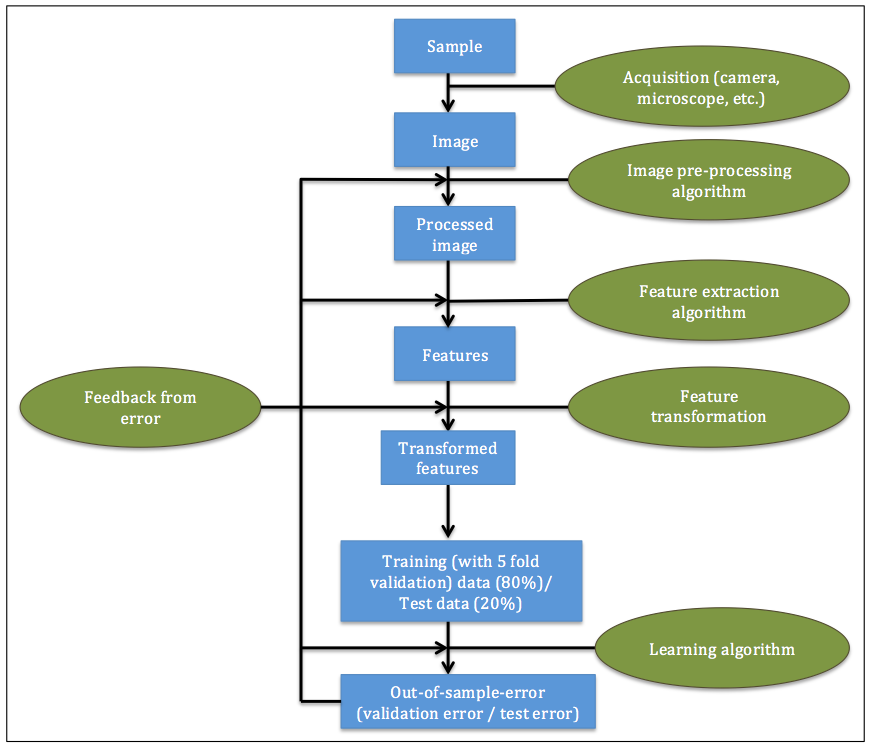
\includegraphics[scale=0.5]{img/EP/flowchart}
    \caption{Representation of an image classification pipeline}
\label{fig:flowchart1}
\end{figure}

the flowchart starts with a sample that is imaged with acquisition technology like a camera or a microscope. The image is then processed using image pre-processing algorithms like normalization and standardization. This may also include image segmentation algorithms. This is followed by feature extraction algorithms that extract useful information from the images. Sometimes, the features extracted are transformed to a different vector space using feature transformation (feature selection or dimensionality reduction) algorithms. The dataset is then divided into training and test datasets in an 80-20 split. Finally, learning algorithms like random forests and logistic regression are used as learning algorithms to build a predictive model for the image classification problem. The performance of the pipeline is evaluated using classification metrics like cross-entropy loss, F1-score, accuracy, precision and recall.  The error in the image classification pipeline maybe measured by such metrics. In this thesis, we base our work on variations of this workflow. Even though the error in image classification pipelines are observed only in terms of the classification error, the source of the error is not just the classification algorithms. The final error is a result of the accumulation of error starting from the beginning of the pipeline right down to the learning algorithms used for classification. Therefore, attempts at improving the performance of image classification pipelines involve the use of  better components in the workflow. This includes using better algorithms and methods for performing data analysis on the image datasets. It may also include improving the quality of the image dataset themselves. Another approach  is to optimize and minimize the error from the pipeline by optimizing the data analytic portion of the pipeline as a whole. This could mean searching the solution space of algorithms to find the best set of algorithms for a particular problem. 
There is also a lack of interpretability of such image classification pipelines, in terms of understanding the source of the errors in the image classification pipeline pertaining to a particular dataset. 
 In this thesis, we present approaches for minimizing the error in image classification with respect to scientific image datasets from different domains. These methods maybe used by domain experts or scientists to train high quality image classification pipelines for similar datasets.  In addition, we also propose methods to quantify the error from all the components of a machine learning pipeline. These methods maybe used by domain experts and data scientists alike to understand and interpret results from image classification pipelines.  

%%% CONTRIBUTIONS
\section{Contributions}
We made the following contributions over the coarse of four projects discussed in the following chapters:
\begin{enumerate}
\item We perform an exhaustive search of data analytic algorithms in the problem of microstructure recognition. The steps included in this work include feature extraction, feature selection and classification algorithms. Each step consists of various algorithms. Two binary image classification tasks are performed in this work. They consist of classification between dendritic and non-dendritic microstructures and between logitudinal and transverse dendrites. We show that this methodology can be used to identify the best configuration of algorithms and hyperparameters in the domain of microstructure recognition.
An exhaustive grid search on the pipeline also shows that pre-trained convolutional neural networks maybe used to represent images of microstructures in the domain of material science

\item We report an automated method for characterization of microvessel morphology by performing data augmentation using parametric 3D models of neuropathological blood vessels. We show that a combination of natural and artificial data perform better in terms of classification metrics.  We propose the development of parametric 3D models of blood vessels and this is used to augment datasets for two classification tasks that involve the classification of morphology of blood vessels. The consist of the classification between singular blood vessels and double blood vessels, and between vessels that consist of lumen and those that don't.

\item We propose a  automated machine learning based score to quantify the quality of an image. This method maybe used to filter a dataset based on the quality of the images. This method can be used by domain experts to perform data analysis on a dataset that only consists of images with a high amount of signal. 

\item We propose an \textit{agnostic} methodology to quantify the contribution of errors from different components of an image classification pipeline. 
We show empirically that performing global random search on the entire pipeline maybe used for efficiently computing the statistics of error contribution from computational steps and algorithms in the image classification pipeline.

\end{enumerate}

%%% OUTLINE
\section{Outline}
The following chapters detail our contributions with respect to optimization and quantification of error in image classification pipelines.
In Chapter \ref{chap:COMMAT}, we describe the problem of microstructure recognition with respect to two classification tasks. 
In Chapter \ref{chap:ISBI}, we propose the parametric 3D model based data augmentation method used in classification of morphologies of blood vessels in neuropathological tissue samples. 
In Chapter \ref{chap:SPIE1}, we present a machine learning based \textit{Quality of Image} score that can automatically quantify whether the image is \textit{good} or \textit{bad}.
In Chapter \ref{chap:EP}, we propose and describe a methodology to quantify the contributions of error from different components of an image classification pipeline. 
In Chapter \ref{chap:conclusions} we present summarized conclusions and discuss relevant future
work. 
\chapter{AN AUTOMATED APPROACH FOR PARALLEL ADJOINT-BASED
ERROR ESTIMATION AND MESH ADAPTATION FOR STEADY-STATE
PROBLEMS}
\label{chap:automated}

\let\thefootnote\relax\footnotetext{
This chapter has been submitted to:
B.~N. Granzow, A.~A. Oberai, and M.~S. Shephard,
``An automated approach for parallel adjoint-based error
estimation and mesh adaptation,'' submitted for publication.}

%%% INTRODUCTION
\section{Introduction}

To make adjoint-based
error estimation and mesh adaptation more accessible to solid mechanics
practitioners, we seek to fully automate its steps for execution on
parallel machines. Specifically, we seek to
develop software that automates steps 1-6 outlined in Chapter \ref{chap:intro}
based solely on the
inputs of a semilinear form $\R$ and a functional QoI $J$. We endeavor to
develop this software to be applicable to both Galerkin and stabilized
finite element methods.

Recently, Rognes and Logg \cite{rognes2013automated} introduced a fully
automated approach to goal-oriented error estimation and mesh adaptation for
Galerkin finite element methods within the FEniCS \cite{logg2012automated}
finite element framework. In this approach, the adjoint problem is derived
in a discrete manner based on a user-implemented residual $\R$ and a
functional $J$. The adjoint problem is then solved on the same finite element
space as used for the primal problem and enriched to a higher order
polynomial space by solving local patch-wise problems.
Based on the given semilinear form
$\R$, error contributions are then localized to the element-level by solving
local element problems to recover the strong form of the residual operator
over element interiors and element boundaries. The total error in the
functional QoI is then computed as the sum of these error contributions. As a
final step, the mesh is adapted using conforming unstructured mesh
\emph{refinement}.

In this work, we present an approach for automating goal-oriented
analysis that is distinct in several ways. First, we consider adjoint-based
error estimation in the context of both Galerkin and stabilized finite element
methods. Additionally, we propose solving the adjoint problem in a richer
finite element space, obtained via uniform refinement, than the space used for
the primal problem. To localize the error to the mesh entity level,
we utilize a partition of unity based approach proposed by Richter
and Wick \cite{richter2015variational}. This allows us to directly re-use the
implemented semilinear form $\R$ for error localization, eliminating the need
to solve local element problems to recover the strong form residual. We also
take advantage of fully unstructured conforming mesh adaptation, where the
mesh can be \emph{coarsened} as well as refined. As a final distinction, we
highlight the ability of the proposed approach to execute on parallel machines.

In totality, our new approach can be described as follows. First, the primal
problem is solved via Newton's method, where the Jacobian of the semilinear
form $\R$ is obtained via automatic differentiation. The adjoint problem is
derived in a discrete manner in a richer finite element space obtained by a
uniform refinement of the initial mesh. The adjoint operator is derived by an
application of automatic differentiation to the semilinear form $\R$, and the
right-hand side of the adjoint problem is obtained by applying automatic
differentiation to the functional $J$. An approximate error $\eta$ is computed
as a modified discrete adjoint weighted residual evaluated on the fine space.
The error is then localized to mesh vertices using a variational localization
approach by introducing a partition of unity into the weighting slot of the semilinear form
$\R$. An approximate upper bound $\hat{\eta}$ is obtained by summing the
absolute values of localized error contributions. Finally, the mesh is adapted
by specifying a \emph{mesh size field}, which defines the length of mesh
edges over the mesh. We have implemented this approach in a \texttt{C++}
finite element application which we have called Goal \cite{goal_github}.

Underlying this approach is the concept of \emph{template-based generic
programming} (TBGP) \cite{pawlowski2012automating1, pawlowski2012automating2},
which has previously been used to automate the solution of PDEs as well as
embedded advanced analysis features, such as
sensitivity analysis and uncertainty quantification. From a high-level the
TBGP approach consists of a \emph{gather} phase, a \emph{compute} phase,
and a \emph{scatter} phase. The present work extends the TBGP approach to
include the automation of error localization, as required to drive
mesh adaptation.

The remainder of this chapter is outlined as follows.
First adjoint-based error estimation is reviewed for abstract
Galerkin and stabilized variational problems.
Next, a description of the software components utilized in this
work is provided. In particular, each step of the automated
adjoint-based analysis is discussed with respect to its utilized software
components. A review of the concept of TBGP is then provided
and its extension for the purposes of adjoint-based error estimation
is discussed. A detailed description of each step in the
adaptive adjoint-based process is then described. First the
automated solution of the primal problem is discussed. Then
the automated derivation and solution of the adjoint problem
is described. Next, the automation of error localization to
drive mesh adaptation is outlined and mesh adaptation procedures
are discussed. The implementation of several QoIs in the Goal
application is reviewed. Finally, the effectiveness of the
proposed automated approach is demonstrated for several
applications.

%%% A REVIEW OF ADJOINT-BASED ERROR REPRESENTATIONS
\section{A Review of Adjoint-Based Error Representations}

In this section, a brief review of the derivation of adjoint-based
error representations is provided for Galerkin finite element methods as
outlined by Becker and Rannacher \cite{becker2001optimal}, and for
stabilized finite element methods as outlined by Cyr et al. \cite{cyr2014approaches}.
This review is inteded to give context and serve as a road map for the remaining
sections in this chapter.

Let $\S$ and $\V$ be Hilbert spaces, $\R_g : \S \to \V$ and
$\R_{\tau} : \S \to \V$ be semilinear forms that are linear in their first
argument and potentially nonlinear in their second argument. Let
$\S^H \subset \S$ and $\V^H \subset \V$ be classical finite element
function spaces, where $H$ is a mesh-dependent parameter that denotes the
fineness of the discretization. We introduce the following variational
abstract model problem: find $u \in \S$ such that
%
%% aut_abstract_primal
\begin{gather}
\R_g(w; u) = 0 \quad \forall w \in \V.
\label{eq:aut_abstract_primal}
\end{gather}
%
Similarly, we introduce the following abstract \emph{adjoint problem}:
find $z \in \V$ such that
%
%% aut_abstract_adjoint
\begin{gather}
\R_g'[u^H](w, z) = J'[u^H](w) \quad \forall w \in \V,
\label{eq:aut_abstract_adjoint}
\end{gather}
%
where the prime indicates Fr\'{e}chet linearization about the argument in
square brackets, which can equivalently be expressed as the G\^{a}teaux
derivatives
%
% aut_functional_deriv
\begin{gather}
J'[u^H](w) :=
\frac{d}{d \epsilon} J(u^H + \epsilon w) \bigr|_{\epsilon = 0},
\end{gather}
%
and
%
%% aut_resid_deriv
\begin{gather}
\R_g'[u^H](w, z) :=
\frac{d}{d \epsilon} \R(z; u^H + \epsilon w) \bigr|_{\epsilon = 0}.
\end{gather}
%
Here, $u^H \in \S^H$ denotes some finite element approximation to the
true solution $u$. The purpose of the adjoint problem is to relate the
original problem of interest to the functional quantity $J$, and it is this
relationship that allows us to derive adjoint-based error representations.
Further, we note that the adjoint solution $z$ can be interpreted as
the sensitivity of the QoI to perturbations in the primal PDE residual
\cite{fidkowski2011review}.

%%% GALERKIN FINITE ELEMENT METHODS
\subsection{Galerkin Finite Element Methods}

The corresponding Galerkin finite element formulation of the abstract
problem \eqref{eq:aut_abstract_primal} can be stated as: find
$u^H \in \S^H$ such that
%
%% aut_abstract_fem
\begin{gather}
\R_g(w^H; u^H) = 0 \quad \forall w^H \in \V^H.
\label{eq:aut_abstract_fem}
\end{gather}
%
Let $e := u-u^H$ denote the discretization error. We can then derive an
error representation for the functional $J$ in terms of the adjoint solution
$z$ as follows:
%
%% aut_abstract_galerkin_error
\begin{gather}
\begin{aligned}
J(u) - J(u^H) &= J'[u^H](e) + \O(e^2) \\
&= \R_g'[u^H](e, z) + \O(e^2) \\
&= \R_g(z; u) - \R_g(z; u^H) + \O(e^2) \\
&= - \R_g(z; u^H) + \O(e^2) \\
&= - \R_g(z - z^H; u^H) + \O(e^2).
\end{aligned}
\label{eq:aut_abstract_galerkin_error}
\end{gather}
%
Here, the first equality is due to the linearization \cite{becker2001optimal}
of the functional $J$, the second equality is due to the introduced adjoint
problem \eqref{eq:aut_abstract_adjoint}, the third equality is due to the
linearization \cite{becker2001optimal} of the residual $\R_g$, the fourth
equality holds due to the definition of the abstract primal problem
\eqref{eq:aut_abstract_primal}, and the fifth equality is due to Galerkin
orthogonality, where $z^H$ denotes the interpolant of $z$ onto the space
$\V^H$. In reference to the notation introduced, the
total residual semilinear form $\R$ is given as $\R = \R_g$.

%%% STABILIZED FINITE ELEMENT METHODS
\subsection{Stabilized Finite Element Methods}

A corresponding stabilized finite element method of the abstract problem
\eqref{eq:aut_abstract_primal} can be expressed as: find $u^H \in \S^H$ such
that
%
%% aut_abstract_stabilized_fem
\begin{gather}
\R_g(w^H; u^H) + \R_{\tau}(w^H; u^H) = 0 \quad \forall w^H \in \V^H.
\label{eq:aut_abstract_stabilized_fem}
\end{gather}
%
Here $\R_{\tau}$ denotes a consistent \emph{stabilization residual} that adds
stability to the numerical scheme. We say that the
stabilization is \emph{consistent} if $\R_{\tau}(w^H ; u) \to 0$ as
$H \to 0$.

Again, we let $e := u - u^H$ denote the discretization error, and derive
an error representation for the functional $J$ as follows
%
%% aut_abstract_stabilized_error
\begin{gather}
\begin{aligned}
J(u) - J(u^H) &= J'[u^H](e) + \O(e^2) \\
&= \R_g'[u^H](e, z) + \O(e^2) \\
&= \R_g(z; u) - \R_g(z; u^H) + \O(e^2) \\
&= - \R_g(z; u^H) + \O(e^2) \\
&= - \R_g(z - z^H; u^H) + \R_{\tau}(z^H; u^H) + \O(e^2).
\end{aligned}
\label{eq:aut_abstract_stabilized_error}
\end{gather}
%
Here, the first four equalities are obtained exactly as in the corresponding
Galerkin finite element method. However, when we subtract the interpolant
$z^H$ of the adjoint solution $z$ in the fifth equality, an additional term
remains because the numerical scheme \eqref{eq:aut_abstract_stabilized_fem}
lacks Galerkin orthogonality. In reference to the notation
introduced, the total semilinear form $\R$ is given as
$\R = \R_g + \R_{\tau}$.

%%% SOFTWARE COMPONENTS
\section{Software Components}

An adaptive adjoint-based simulation
requires the implementation and coordination of a number of
non trivial components. Namely, the solution of a primal problem,
the construction and solution of an auxiliary adjoint problem, an enrichment
of the adjoint solution, the estimation and localization of the error,
and mesh adaptation are all required steps in the adjoint-based
adaptive process.

To implement each of these components for effective execution on parallel
machines, we make use of two state of the art software suites. The first
is PUMI \cite{ibanez2016pumi}, which contains tools to
support unstructured mesh services on massively parallel machines. In
particular, PUMI provides all of the necessary machinery to store, query,
adapt, and dynamically load balance parallel unstructured meshes via
a collection of modern \texttt{C} and \texttt{C++} libraries. The second
is Trilinos \cite{heroux2005overview, heroux2012new}, which provides a
large variety of \texttt{C++} packages to support multiphysics
simulations on parallel machines. In particular, Trilinos provides
the ability to store and solve sparse parallel linear systems, as
well as tools to perform automatic differentiation.

Using these two software suites as building blocks, we have written a new
\texttt{C++} application for adjoint-based error estimation and mesh
adaptation with an emphasis on nonlinear solid mechanics. We have called this
application Goal \cite{goal_github}. Below, we describe
how these software components are
utilized for each portion of the adaptive adjoint-based process,
where the analysis is automated based only on the inputs of a semilinear
form $\R$ and a functional QoI $J$.

%%% THE PRIMAL PROBLEM
\subsection{The Primal Problem}

Based on an implemented weighted residual operator $\R$, the Goal
application computes element-level residual vectors and element-level
Jacobian matrices. The element-level Jacobian matrices are computed via
automatic differentiation using the Trilinos library Sacado. Sacado
provides efficient automatic differentiation using a \texttt{C++}
meta-programming technique called expression templates
\cite{phipps2012efficient}.

After the computation of a single element's residual vector and Jacobian
matrix, the Goal application performs a finite element assembly step to
sum contributions to the global residual vector and global Jacobian matrix.
To store and modify the global linear algebra objects, we utilize the Tpetra
library provided by Trilinos. In particular, the Jacobian matrix is stored
as a sparse compressed row storage matrix in parallel.

The primal problem is solved via Newton's method, which requires iterative
evaluations of the global residual vector and Jacobian matrix. For each
Newton iteration, a global linear system must be solved. We solve
this linear system iteratively in parallel using either a CG or GMRES solver provided
the Trilinos library Belos \cite{bavier2012amesos2}. Additionally, we
perform algebraic multigrid preconditioning using the Trilinos library
MueLu \cite{MueLu}.

Once the primal problem has been solved, we utilize the PUMI library APF
to store the finite element solution information at nodes and if necessary
secondary solution information at integration points. Additionally, the APF
library is used to provide shape function information and to query stored
solution information during residual and Jacobian evaluations. Throughout
the entire solution process, the PUMI mesh data structure is utilized to
query mesh specific information.

%%% THE ADJOINT PROBLEM
\subsection{The Adjoint Problem}

To solve the adjoint problem in a richer finite element space than the one
used for the primal problem, we make use of the underlying PUMI mesh data
structure \cite{ibanez2017modifiable} and the PUMI MeshAdapt software to
create and store a uniformly refined nested mesh with parent-child relations
back to the original mesh. This relational information is implemented in the
Goal application, as it falls outside of the normal intended use case of the
MeshAdapt software, which concerns itself with fully unstructured conforming
mesh adaptation via edge splits, swaps, and collapses. However,
the flexibility of the PUMI software allows us to
additionally construct data structures similar to those used in traditional
adaptive mesh refinement (AMR) with little implementation effort. Using
the APF library and the parent-child relational information, we are able
to interrogate stored solution fields on both the parent and nested meshes,
which is required during the assembly of the adjoint problem.

On this finer mesh, element-level Jacobian matrices are computed using the
Sacado library, based on the Goal implementation of the operator $\R$.
Additionally, element-level derivatives of the functional quantity of
interest $J$ are computed with respect to degrees of freedom of the problem,
resulting in an element-level functional derivative vector.

After the computation of a single element's Jacobian matrix and functional
derivative vector, the Goal application performs a finite element assembly
step to sum contributions to the global discrete adjoint matrix and the
global functional derivative vector. Like the primal problem, these global
parallel linear objects are stored using the Tpetra library. The global
discrete adjoint operator and functional derivative vector fully define the
linearized adjoint problem, which we again precondition with algebraic
multigrid techniques using the MueLu library and solve using either CG
or GMRES iterations using the Belos library. The fine-space adjoint solution
is then attached to the mesh using the APF library.

%%% ERROR ESTIMATION AND LOCALIZATION
\subsection{Error Estimation and Localization}

The error estimation and localization routines are implemented entirely in
the Goal application. The error is localized by an evaluation of the
stabilized weighted residual operator $\R$, where the weight is chosen to be
the adjoint solution multiplied by a partition of unity. Based on these
element-level residual vectors, Goal performs finite element assembly
of the global residual vector, which is stored as a Tpetra vector. This
vector represents an adjoint-weighted residual error estimate at each mesh
vertex for each PDE equation in the fine mesh. The error is attached to the
vertices of the fine mesh using the APF library.

%%% MESH ADAPTATION
\subsection{Mesh Adaptation}

Once the error is stored on the vertices of the fine mesh, we interpolate
it to element centers of the coarse mesh. The fine mesh data structures are
then destroyed and the Goal application computes a mesh size field that
seeks to equidistribute the error for an output mesh with $N$ elements. This
mesh size field is given as the input to the PUMI MeshAdapt software, which
adapts the mesh with a sequence of edge splits, swaps, and collapses
\cite{li20053d, alauzet2006parallel} to satisfy the given mesh size field.
As a final step, we utilize the PUMI library ParMA
\cite{smith2015parma, diamond2017dynamic}
to perform diffusive
load balancing to ensure parallel partitioning quality.

%%% IN-MEMORY INTEGRATION
\subsection{In-Memory Integration of Components}

The coupling of both the analysis and
software components described above is done \emph{in-memory}
\cite{smith2016memory}. That is, there is no file-based communication of
data from one analysis component to the next in the automated process.
This in-memory coupling is a key ingredient for parallel analysis,
where filesystem bandwidth is a critical bottleneck.

%%% TEMPLATE-BASED GENERIC PROGRAMMING
\section{Template-Based Generic Programming}
\label{sec:tbgp}

In this section, we provide a review of the concept of
\emph{template-based generic programming} for the evaluation and solution of
PDEs \cite{pawlowski2012automating1,pawlowski2012automating2} and how it
has been extended in the Goal application to automate the process of
adjoint-based error estimation and mesh adaptation. 
For PDE applications, TBGP is broken into three major components,
a \emph{seed} or \emph{gather} phase, a \emph{compute} phase, and
a \emph{scatter} phase. The seed and scatter operations must be
programmed specifically for each evaluation purpose. In contrast, the
compute phase, where the PDE and QoI expressions are implemented,
are written in a totally generic manner. Figure \ref{fig:mech_tbgp}
pictorially represents this design philosophy.

\begin{figure}[ht!]
\centering
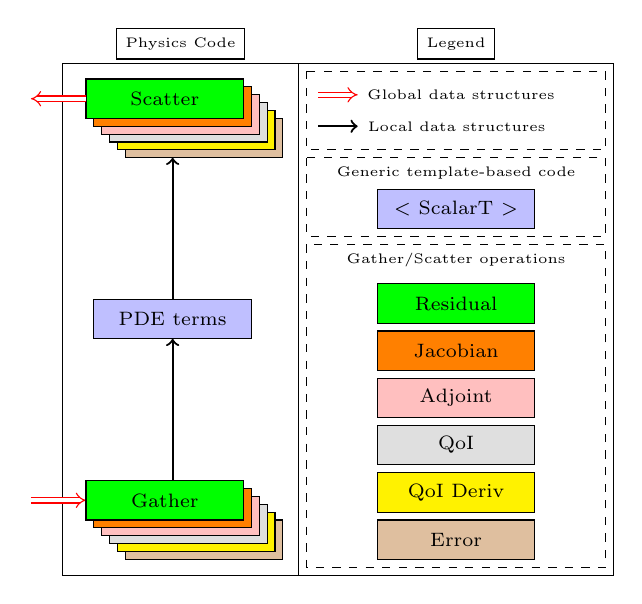
\begin{tikzpicture}

% physic code
\node[draw] at (1.5,6.25) {\tiny Physics Code};

% legend
\node[draw] at (5, 6.25) {\tiny Legend};

% bounding boxes
\draw (0,-0.5) rectangle +(3, 6.5);
\draw (3,-0.5) rectangle +(4, 6.5);

% global data transfer -> gather
\draw[red,-implies,double equal sign distance] (-0.4,0.45) -- (0.3,0.45);

% gather template operations
\draw[fill=brown!50] (0.8, -0.3) rectangle+(2,0.5);
\draw[fill=yellow] (0.7, -0.2) rectangle+(2,0.5);
\draw[fill=gray!25] (0.6, -0.1) rectangle+(2,0.5);
\draw[fill=pink] (0.5, 0.0) rectangle+(2,0.5);
\draw[fill=orange] (0.4, 0.1) rectangle+(2,0.5);
\draw[fill=green] (0.3, 0.2) rectangle +(2,0.5)
node[pos=0.5] {\scriptsize Gather};

% local data transfer gather -> pde
\draw[black,thick,->] (1.4,.7) -- (1.4,2.5);

% generic template pde evaluation
\draw[fill=blue!25] (0.4,2.5) rectangle +(2,0.5)
node[pos=0.5] {\scriptsize PDE terms};

% local data transfer pde -> scatter
\draw[black,thick,->] (1.4,3.0) -- (1.4,4.8);

% scatter template operations
\draw[fill=brown!50] (0.8, 5.3) rectangle+(2,-0.5);
\draw[fill=yellow] (0.7, 5.4) rectangle+(2,-0.5);
\draw[fill=gray!25] (0.6, 5.5) rectangle+(2,-0.5);
\draw[fill=pink] (0.5, 5.6) rectangle+(2,-0.5);
\draw[fill=orange] (0.4, 5.7) rectangle+(2,-0.5);
\draw[fill=green] (0.3, 5.8) rectangle+(2,-0.5)
node[pos=0.5] {\scriptsize Scatter};

% global data transfer <- scatter
\draw[red,implies-,double equal sign distance] (-0.4,5.55) -- (0.3,5.55);

% data transfer
\draw[dashed] (3.1,5.9) rectangle +(3.8,-1);
\draw[red,-implies,double equal sign distance] (3.25,5.6) -- (3.75,5.6)
node[black,anchor=west] {\tiny Global data structures};
\draw[black,thick,->] (3.25, 5.2) -- (3.75, 5.2)
node[black,anchor=west] {\tiny Local data structures};

% generic data evaluation type
\draw[dashed] (3.1, 4.8) rectangle +(3.8,-1);
\node[black] at (5,4.6) {\tiny Generic template-based code};
\draw[fill=blue!25] (4,4.4) rectangle +(2,-0.5)
node[pos=0.5] {\scriptsize $<$ ScalarT $>$};

% template specializations
\draw[dashed] (3.1, 3.7) rectangle +(3.8,-4.1);
\node[black] at (5,3.5) {\tiny Gather/Scatter operations};
\draw[fill=green] (4,3.2) rectangle +(2,-0.5)
node[pos=0.5] {\scriptsize Residual};
\draw[fill=orange] (4,2.6) rectangle +(2,-0.5)
node[pos=0.5] {\scriptsize Jacobian};
\draw[fill=pink] (4,2.0) rectangle +(2,-0.5)
node[pos=0.5] {\scriptsize Adjoint};
\draw[fill=gray!25] (4,1.4) rectangle +(2,-0.5)
node[pos=0.5] {\scriptsize QoI};
\draw[fill=yellow] (4,0.8) rectangle +(2,-0.5)
node[pos=0.5] {\scriptsize QoI Deriv};
\draw[fill=brown!50] (4,0.2) rectangle +(2,-0.5)
node[pos=0.5] {\scriptsize Error};
\end{tikzpicture}

\caption{A schematic for the generic programming model of PDEs.}
\label{fig:mech_tbgp}
\end{figure}

We invoke this approach at the element-level, meaning for each element
we perform the process: Gather $\rightarrow$ Compute $\rightarrow$
Scatter. By doing so, we reduce memory overhead and eliminate complications
introduced by parallel computation \cite{pawlowski2012automating2}.
Underlying the TBGP approach is the use of forward automatic differentiation
(FAD) \cite{griewank2008evaluating}, which is discussed in further detail
in Appendix \ref{chap:fad}. The Goal application utilizes the
Trilinos library Sacado \cite{phipps2012efficient} to perform
automatic differentiation.

\begin{table}[ht!]
\tabulinesep=1.2mm
\centering
\begin{tabu}{| l |  l | c | c |} \hline
Evaluation Type & Scalar Type & Input & Output \\ \hline \hline
Residual & \texttt{double} & $\bs{u}^H, \bs{s}^H$ & $\bs{R}^H$ \\ \hline
Jacobian & \texttt{Sacado::FAD} & $\bs{u}^H, \bs{s}^H$ & $\frac{\partial \bs{R}^H}{\partial \bs{u}^H}$ \\ \hline
Adjoint & \texttt{Sacado::FAD} & $\bs{u}^h_H, \bs{s}^h_H$ & $\left[ \frac{\partial \bs{R}^h}{\partial \bs{u}^h} \bigr|_{\bs{u}^h_H} \right]^T$ \\ \hline
QoI & \texttt{double} & $\bs{u}^H, \bs{s}^H$ & $J^H$ \\ \hline
QoI Deriv & \texttt{Sacado::FAD} & $\bs{u}^h_H, \bs{s}^h_H$ & $ \left[ \frac{ \partial J^h} { \partial \bs{u}^h} \bigr|_{\bs{u}^h_H} \right]^T $ \\ \hline
Error & \texttt{double} & $\bs{u}^h_H, \bs{s}^h_H, \bs{z}^h$ & $\bs{R}^h$ \\ \hline
\end{tabu}
\caption{A list of TBGP evaluation operations used in the Goal application.
In this table $\bs{u}^H$ is the primal solution vector, $\bs{u}^h_H$ is the
prolongation of the solution vector to a richer space, $\bs{s}^H$ is a
(potentially empty) vector of history-dependent mechanics state variables,
$\bs{s}^h_H$ is the prolongation of the state to a richer space,
$\bs{z}^h$ is the adjoint solution vector,
$\bs{R}^H$ is the residual vector evaluated on the coarse space,
$\bs{R}^h$ is the residual vector evaluated on the fine space, and
$J^H$ is the scalar QoI.}
\label{tab:software_evaluations}
\end{table}

The purpose of the gather/seed operation is to collect information
from global storage containers and `gather' it to local element-level
data structures. Further, any FAD derivative information is \emph{seeded}
during this operation, if necessary. For each evaluation type, the
gather/seed operation initializes an array that physically represent the
degrees of freedom associated with the current element, and
initializes FAD variables' derivative arrays to physically represent
derivatives with respect to the degrees of freedom associated with
the current element, when necessary. This degree of freedom array is
templated on a scalar type \texttt{ScalarT}. For the Residual, QoI,
and Error evaluation types, this scalar type corresponds to a
\texttt{C++} double. For the remaining evaluation types, this
scalar type corresponds to a \texttt{Sacado::FAD} forward automatic
differentiation variable type.

The compute phase computes local contributions to the equations or
expressions of interest at the element level in terms of the degrees
of freedom, as collected by the gather operation. The code for the
compute phase is written in an entirely generic fashion, and is templated
on a scalar type \texttt{ScalarT}. Templating the code used for the
compute phase, along with appropriately chosen gather and scatter
operations, allows the same code to be re-used for the distinct
evaluation purposes listed in Table \ref{tab:software_evaluations}.

The scatter phase takes the local element-level data
evaluated in the compute phase and `scatters' it to the appropriate
global data structure, as determined by the current evaluation operation.
For instance, for the residual evaluation operation, local element-level
residuals are evaluated in the compute phase and then summed into
appropriate locations in the global residual vector during the scatter
phase. Similarly, for the Jacobian evaluation operations, local element-level
Jacobians are evaluated in the compute phase and the scatter opeation
sums these local contributions to appropriate locations in the global
Jacobian matrix.

\begin{lstlisting}[
float,
style=mystyle,
caption=The abstract Goal integrator class interface,
label=lst:software_integrator]
class Integrator {
  public:
    Integrator();
    virtual ~Integrator();
    std::string const& get_name() { return name; }
    virtual void set_time(double, double) {}
    virtual void pre_process(SolInfo*) {}
    virtual void set_elem_set(int) {}
    virtual void gather(apf::MeshElement*) {}
    virtual void in_elem(apf::MeshElement*) {}
    virtual void at_point(apf::Vector3 const&, double, double) {}
    virtual void out_elem() {}
    virtual void scatter(SolInfo*) {}
    virtual void post_process(SolInfo*) {}
  protected:
    std::string name;
\end{lstlisting}

In the Goal application, we have considered six specific gather/scatter
evaluation operations corresponding to the evaluation of the global
residual vector, evaluation of the global Jacobian matrix, evaluation
of the adjoint of the global Jacobian matrix, evaluation of the
functional QoI, evaluation of the derivative of the functional QoI,
and evaluation of localized adjoint-weighted residual error estimates.
Table \ref{tab:software_evaluations} lists the inputs and outputs for
these specific evaluation operations.

To realize these specific gather/scatter operations, we have implemented
an abstract degree of freedom class and an abstract quantity of interest
class that are both templated on a scalar type \texttt{ScalarT}. This
scalar type is explicitly instantiated to either be a \texttt{C++} double
or a \texttt{Sacado::FAD} forward automatic differentiation variable type.
Both the degree of freedom and QoI classes are equipped with \texttt{gather}
and \texttt{scatter} methods, whose behavior changes based on an input
parameter given to the class constructor. For the degree of freedom
class, this parameter selects gather/scatter operations for either the
residual, Jacobian, adjoint Jacobian, or adjoint-weighted residual error
evaluations. Similarly, for the QoI class, this input parameter selects
gather/scatter operations for either the evaluation of the QoI
or the derivative of the QoI with respect to the problem degrees of freedom.

Previously, TBGP has been utilized in the multiphysics code
Albany \cite{salinger2013albany, tezaur2015albany} with the capability
to perform the Residual, Jacobian, Adjoint, QoI, and QoI derivative
evaluation operations shown in Table \ref{tab:software_evaluations}.
To extend the abilities of TBGP to include adjoint-based error estimation,
the Goal application implements the ability to perform the Adjoint and
QoI derivative evaluations in a richer finite element space, as
discussed in Section \ref{sec:aut_adjoint}, a feature not previously
available in existing TBGP codes. Further, the Goal application implements a
novel evaluation type for the localization of the error, referred to as the
Error evaluation type in Table \ref{tab:software_evaluations}. For this purpose,
we have implemented an abstract weighting function class whose
behavior changes based on the chosen evaluation type. This class
evaluates the appropriate finite element weighting function values
and gradients based on linear Lagrange basis functions for the
Residual, Jacobian and Adjoint evaluation types. However, for the
Error evaluation type, the behavior of the weighting function
class is modified such that it evaluates the value and gradient
of the adjoint solution $z^h$ multiplied by a partition of unity. This abstraction of the
weighting function class
allows us to re-use the PDE implementation of the semilinear form
$\R$ to assemble a residual vector $\bs{R}^h$ that represents an
adjoint-weighted residual error estimate at each mesh vertex for each PDE
equation in the richer finite element space, which is then used
to drive mesh adaptation.

Listing \ref{lst:software_integrator} demonstrates the abstract
integrator interface that has been implemented in the Goal
application. The abstract degree of freedom, QoI, and
weighting function classes inherit from this base class.
For each of these classes, the \texttt{gather} and \texttt{scatter}
methods are implemented specifically for each appropriate
evaluation type. The PDE equations in the Goal application are
written as a combination of \texttt{Goal::Integrator}s.
Given  an ordered array of integrators, the Goal application
performs finite element assembly for every evaluation type
in a generic manner, as outlined by Algorithm \ref{alg:software_assembly}.

\begin{algorithm}
\caption{Assembly algorithm used in the Goal application}
\begin{algorithmic}
\State Given a mesh $M$ and an ordered array of integrators $I$:
\State Call \texttt{pre\_process} for each integrator $i$ in $I$.
\For{ each element set $es$ in mesh $M$ }
\State Call \texttt{set\_elem\_set} for each integrator $i$ in $I$.
\For{ each element $e$ in element set $es$ }
\State Call \texttt{gather} for each integrator $i$ in $I$.
\State Call \texttt{in\_elem} for each integrator $i$ in $I$.
\For{ each integration point $ip$ in element $e$ }
\State Call \texttt{at\_point} for each integrator $i$ in $I$.
\EndFor
\State Call \texttt{out\_elem} for each integrator $i$ in $I$.
\State Call \texttt{scatter} for each integrator $i$ in $I$.
\EndFor
\EndFor
\State Call \texttt{post\_process} for each integrator $i$ in $I$.
\end{algorithmic}
\label{alg:software_assembly}
\end{algorithm}

%%% THE PRIMAL PROBLEM
\section{The Primal Problem}

%%% GALERKIN FINITE ELEMENT METHODS
\subsection{Galerkin Finite Element Methods}

We recall the definition of the abstract Galerkin finite element model
problem, given by equation \eqref{eq:aut_abstract_fem}. In this context,
the weighted residual form $\R_g$ is implemented in the Goal application.
As an example, Listing \ref{lst:presidual} demonstrates the implementation
of the Poisson residual $\R_g(w; u) := (\nabla w, \nabla u) - (w,f)$ in
the Goal application.

\begin{lstlisting}[
float,
style=mystyle,
caption=Poisson residual,
label=lst:presidual]
template <typename ScalarT>
void Residual<ScalarT>::at_point(
    apf::Vector3 const& p, double ipw, double dv) {
  apf::Vector3 x(0,0,0);
  apf::mapLocalToGlobal(elem, p, x);
  double fval = eval(f, x[0], x[1], x[2], 0.0);
  for (int n = 0; n < u->get_num_nodes(); ++n)
  for (int i = 0; i < num_dims; ++i)
    u->resid(n) += u->grad(i) * w->grad(n, i) * ipw * dv;
  for (int n = 0; n < u->get_num_nodes(); ++n)
    u->resid(n) -= fval * w->val(n) * ipw * dv;
}
\end{lstlisting}

%%% STABILIZED FINITE ELEMENT METHODS
\subsection{Stabilized Finite Element Methods}

We recall the definition of the abstract stabilized finite element model
problem, given by equation \eqref{eq:aut_abstract_stabilized_fem}. In this
context, both the weighted residual statement $\R_g$ and the stabilized
weighted residual form $\R_{\tau}$ are implemented in the Goal application.
As an example, Listing \ref{lst:stabresidual} demonstrates the implementation
of the pressure stabilization \cite{ramesh2005stabilized} residual
$\R_{\tau}(w; u)$ term used in the Goal application for finite deformation
solid mechanics.

\begin{lstlisting}[
float,
style=mystyle,
caption=Pressure stabilization residual for mechanics,
label=lst:stabresidual]
template <typename ScalarT>
void Stabilization<ScalarT>::at_point(
    apf::Vector3 const&, double ipw, double dv) {
  double h = get_size(mesh, elem);
  double tau = 0.5*c0*h*h/mu;
  auto J = k->get_det_def_grad();
  auto F = k->get_def_grad();
  auto Cinv = inverse(transpose(F)*F);
  for (int n = 0; n < p->get_num_nodes(); ++n)
  for (int i = 0; i < num_dims; ++i)
  for (int j = 0; j < num_dims; ++j)
    p->resid(n) += tau * J * Cinv(i, j) *
      p->grad(i) * w->grad(n, j) * ipw * dv;
}
\end{lstlisting}

%%% AUTOMATED SOLUTION BASED ON RESIDUAL IMPLEMENTATION
\subsection{Automated Solution Based on Residual Implementation}

For each element, we compute element level
Jacobian matrices by applying automatic
differentiation \cite{griewank2008evaluating} to element-level contributions
to the residual vector. For example, Listing \ref{lst:presidual} demonstrates
how contributions to the element-level Poisson's equation residual
$\R(w; u) = (\nabla w, \nabla u) - (w, f)$ are implemented. The element level
Jacobian matrices are then assembled into the global system Jacobian operator
$\bs{\J}^H \in \mathbb{R}^{N \times N}$, given by
%
%% aut_jacobian
\begin{gather}
\bs{\J}^H = \frac{\partial \bs{R}^H (\bs{u}^H) }{\partial \bs{u}^H}
\end{gather}

Listings \ref{lst:presidual} and \ref{lst:stabresidual} both demonstrate how
element-level contributions to the semilinear forms $\R_g$ and $\R_{\tau}$,
respectively, are computed in the Goal application. Notice that this code
is templated on a scalar type \texttt{ScalarT}. When the scalar type is
chosen as a \texttt{C++} \texttt{double}, element-level contributions to
the residual vector $\bs{R}^H$ are computed. When the scalar type is chosen
as a Sacado forward automatic differentiation variable, element-level
contributions to the Jacobian matrix $\bs{\J}^H$ are computed. This
illustrates a key concept of template-based generic programming, in that
the governing equations need only be implemented once to compute a variety
of additional information.

With the ability to fully assemble the Jacobian matrix $\bs{\J}^H$ and the
residual vector $\bs{R}^H$, we solve the governing equations with Newton's
method, where we iterate over the steps
%
%% aut_netwon
\begin{gather}
\begin{aligned}
\bs{\J}^H (\bs{u}^H_k) \, \delta \bs{u}^H_k &=
- \bs{R}^H( \bs{u}^H_k) \\
\bs{u}^H_{k+1} &= \bs{u}^H_k + \delta \bs{u}^H_k,
\end{aligned}
\end{gather}
%
unitl the convergence criterion $\| \bs{R}^H(\bs{u}^H) \|_2 < \epsilon$ is met
for a user-specified tolerance $\epsilon$. Here $\bs{u}^H_k$ denotes the
solution vector at the $k^{th}$ iteration obtained by solving the Newton
linear system. For linear variational problems, we simply restrict ourselves
to a single Newton linear solve, which reduces exactly to classical FEM
assembly for linear problems.

%%% THE ADJOINT PROBLEM
\section{The Adjoint Problem}
\label{sec:aut_adjoint}

%%% A RICHER SPACE VIA UNIFORM REFINEMENT
\subsection{A Richer Space via Uniform Refinement}

The adjoint solution must be represented in a richer
space than the one used for the primal problem to obtain meaningful error
estimates. There are several strategies that are commonly used to obtain
such a representation. First, the adjoint problem can be solved in the same
finite element space as the primal problem and then be enriched to a higher
order polynomial space \cite{becker2001optimal} or a nested mesh
\cite{nemec2007adjoint} by some local patch-wise operation, or variational
multiscale enrichment \cite{granzow2017output} can be used in the context
of stabilized finite elements. Alternatively, the adjoint problem can be solved in a
higher order polynomial space \cite{fidkowski2011output}, which we will refer
to as $p$-enrichment. As a final option, the adjoint problem can be solved on a
uniformly refined mesh \cite{burstedde2009parallel}, which we will refer to
as $h$-enrichment.

In this work, we choose the $h$-enrichment approach for several reasons.
First, we would like the adjoint solution to be as accurate as possible
for error estimation purposes, so we choose to solve the adjoint problem in
a globally richer finite element space. Additionally, for stabilized finite
element methods, the use of $p$-enrichment would in general necessitate the
use of higher order stabilization terms that vanish for lower-order finite
element methods with simplical elements. These higher order terms are
typically more difficult to implement than their lower order counterparts.
Further, we remark that higher-order stabilized finite element methods are
rarely used in practice, as stable higher-order mixed methods can usually
be derived with fewer overall degrees of freedom \cite{taylor1973numerical}.
Finally, we note that the unstructured mesh adaptation capabilities of the
PUMI software make the $h$-enrichment approach readily available.

We have denoted the trial and test spaces used for the primal problem
as $\S^H$ and $\V^H$, respectively. We denote the trial and test spaces on
the uniformly nested mesh as $\S^h$ and $\V^h$, respectively, where $h < H$
is representative of a finer mesh size. Figure \ref{fig:aut_glial_nested}
illustrates the discretization for the coarse and fine trial and test spaces
defined for a three dimensional geometry with a complex void inclusion.

\begin{figure}[ht!]
\centering
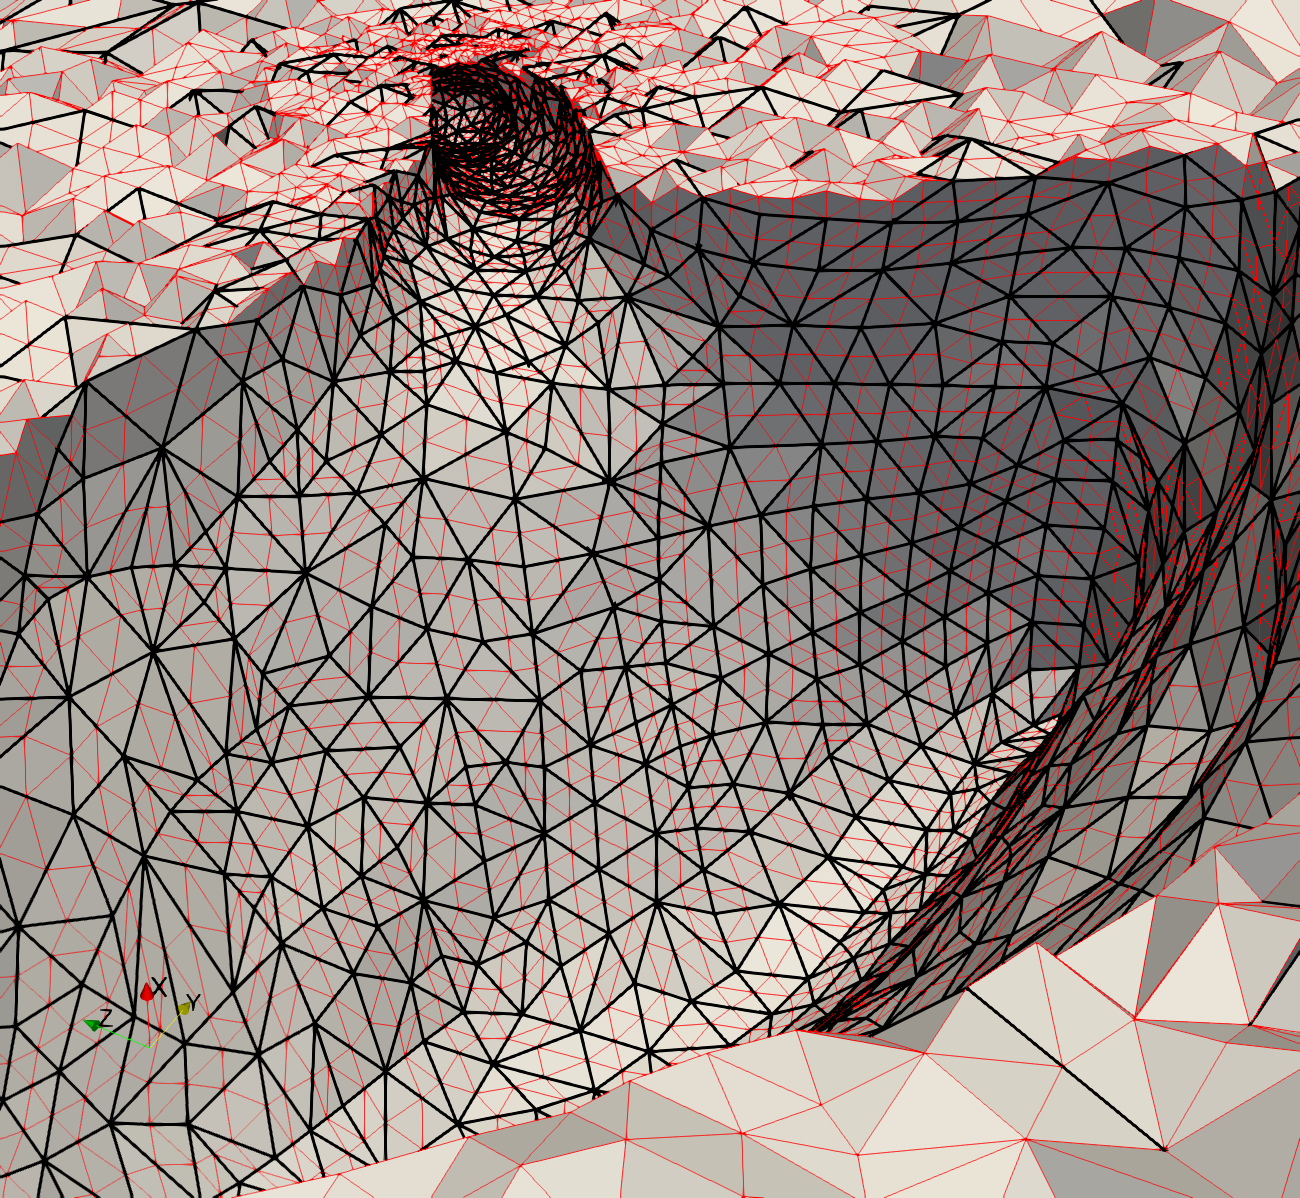
\includegraphics[width=0.5\textwidth]{img/aut_glial_nested}
\caption{Example of a nested mesh (red edges) obtained via a uniform
refinement of a base mesh (black edges) in three dimensions.}
\label{fig:aut_glial_nested}
\end{figure}

%%% DISCRETE ADJOINT APPROXIMATION
\subsection{Discrete Adjoint Approximation}

Let $\bs{R}^h : \mathbb{R}^n \to \mathbb{R}^n$ denote the residual form of
the system of nonlinear algebraic equations arising either from the Galerkin
\eqref{eq:aut_abstract_fem} or stabilized
\eqref{eq:aut_abstract_stabilized_fem}
model problem posed on the uniformly nested mesh. Let $\bs{u}^h_H :=
I^h_H \bs{u}^H$ denote the prolongation of the primal finite element solution
onto the richer space $\S^h$ via interpolation,
Let $J^h : \mathbb{R}^n \to
\mathbb{R}$ denote the discretization of the functional QoI on the
uniformly nested fine space. We approximate the adjoint problem
\eqref{eq:aut_abstract_adjoint} in a discrete manner
\cite{fidkowski2011review, venditti2000adjoint, venditti2002adjoint,
venditti2003adjoint}, by solving
%
%%
\begin{gather}
\left[ \frac{\partial \bs{R}^h}{\partial \bs{u}^h} \biggr|_{u^h_H}
\right]^T \bs{z}^h = \left[ \frac{\partial J^h}{\partial \bs{u}^h}
\biggr|_{u^h_H} \right]^T.
\label{eq:aut_discrete_adjoint}
\end{gather}
%
This allows us to automate the process of solving the adjoint problem, as
discussed below. Here $\bs{z}^h \in \mathbb{R}^n$ denotes the adjoint
solution vector on the nested discretization.

%%% AUTOMATED SOLUTION BASED ON RESIDUAL FORMULATION
\subsection{Automated Solution Based on Residual Formulation}

The construction of the Jacobian transpose matrix $\left[ \partial \bs{R}^h
/ \partial \bs{u}^h \right]^T$ is performed in the same automated manner as
the Jacobian for the primal problem. That is, for each element, we compute
consistent element tangent stiffness matrices via automatic differentiation
of element-level contributions to the residual vector. However, during the
\emph{scatter} phase of the template-based generic programming process,
we transpose the element-level tangent matrices and
sum them into global Jacobian adjoint matrix. The computation of the Jacobian
adjoint is done using the same templated code that is used to compute
the primal residual vector and the Jacobian matrix, as illustrated by
listings \ref{lst:presidual} and \ref{lst:stabresidual}.

Similarly, the construction of the functional derivative vector
$\left[ \partial J^h / \partial \bs{u}^h \right]^T$ is done by evaluating
derivatives of element-level contributions to the functional via automatic
differentiation. This results in element-level derivative vectors that are
then assembled into the global functional derivative vector. Listings
\ref{lst:aut_avg_u_qoi} and \ref{lst:aut_avg_vm_qoi} illustrate the
implementation of two quantities of interest in the Goal application. Once
the Jacobian transpose matrix and functional derivative vector have been
assembled, we solve the adjoint problem \eqref{eq:aut_discrete_adjoint} using
a sparse iterative solver in parallel.

%%% ERROR ESTIMATION
\section{Error Estimation}

%%% TWO LEVEL ERROR ESTIMATES
\subsection{Two-Level Error Estimates}

Following Venditti and Darmofal
\cite{venditti2000adjoint, venditti2002adjoint, venditti2003adjoint},
we review adjoint-based error estimation using two discretization levels.
The discrete residual form of the governing equations for a Galerkin
\eqref{eq:aut_abstract_fem} finite element method or a stabilized finite
element method \eqref{eq:aut_abstract_stabilized_fem} posed on the fine
space can be expressed as
%
%% aut_fine_resid
\begin{gather}
\bs{R}^h(\bs{u}^h) = \bs{0}.
\label{eq:aut_fine_resid}
\end{gather}
%

Taking Taylor expansions of the discrete residual $\bs{R}^h$ evaluated on the
fine space and the discrete functional $J^h$ evaluated on the fine space
about the point $\bs{u}^h_H$ yields
%
%% aut_residual_taylor
\begin{gather}
\bs{R}^h(\bs{u}^h) = \bs{R}^h(\bs{u}^h_H) +
\left[ 
\frac{ \partial \bs{R}^h }{ \partial \bs{u}^h} \biggr|_{\bs{u}^h_H}
\right]
(\bs{u}^h - \bs{u}^h_H) + \dots
\label{eq:aut_residual_taylor}
\end{gather}
%
and
%
%
%% aut_functional_taylor
\begin{gather}
J^h(\bs{u}^h) = J^h(\bs{u}^h_H) +
\left[
\frac{ \partial J^h } { \partial \bs{u}^h} \biggr|_{\bs{u}^h_H}
\right]
(\bs{u}^h - \bs{u}^h_H) + \dots
\label{eq:aut_functional_taylor}
\end{gather}
%
respectively.

Using equation \eqref{eq:aut_fine_resid}, the discretization error
between the two spaces can be approximated to first order as
%
%% aut_disc_error_approx
\begin{gather}
(\bs{u}^h - \bs{u}^h_H) \approx
- \left[
\frac{ \partial \bs{R}^h } { \partial \bs{u}^h } \biggr|_{\bs{u}^h_H}
\right]^{-1}
\bs{R}^h (\bs{u}^h_H ),
\label{eq:aut_disc_error_approx}
\end{gather}
%
which can then be substituted into the functional Taylor expansion
\eqref{eq:aut_functional_taylor} to obtain the so-called
\emph{adjoint weighted residual}
%
%% 
\begin{gather}
J^h(\bs{u}^h) - J^h(\bs{u}^h_H) \approx  - \bs{z}^h \cdot \bs{R}^h(\bs{u}^h_H)
\label{eq:aut_adjoint_weighted_residual}
\end{gather}
%
where $\bs{z}^h$ is the solution to the adjoint problem
\eqref{eq:aut_discrete_adjoint}.

%%% MODIFIED FUNCTIONAL ERROR ESTIMATE
\subsection{Modified Functional Error Estimate}

Assume that the QoI converges at the rate $k$, such that
$J - J^h(\bs{u}^h_H) = c H^k$ and $J - J^h(\bs{u}^h) = ch^k$,
where $J$ denotes the exact value of the QoI. If the fine space
is obtained via uniform mesh refinement, then the ratio of the fine mesh size
to the coarse mesh size is given as $\frac{h}{H} = \frac12$. Consider the ratio
%
%% aut_ratio
\begin{gather}
\begin{aligned}
\frac{ J^h (\bs{u}^h) - J^h(\bs{u}^h_H) }{ J - J^h(\bs{u}^h_H) }
&= \frac{\left[ J - J^h(\bs{u}^h_H) \right] -
\left[ J - J^h(\bs{u}^h) \right] }
{ J - J^h(\bs{u}^h_H) } \\
&= \frac{c H^k - ch^k}{c H^k} \\
&= 1 - \left( \frac{h}{H} \right)^k \\
&= 1 - \left( \frac12 \right)^k
\end{aligned}
\end{gather}
%
in the limit as $H \to 0$ \cite{fidkowski2011review}. We call this
ratio $\alpha := 1 - (1/2)^k$. Let $\eta$ denote an approximation
to the functional error $J - J^h(\bs{u}^h_H)$. Let $\I$
denote the effectivity index given by
%
%% aut_effectivity
\begin{gather}
\I = \frac{\eta}{ J - J^h(\bs{u}^h_H) }.
\label{eq:aut_effectivity}
\end{gather}
%
We would like to obtain error estimates $\eta$ that lead to
effectivity indices of $\I = 1$ as $H \to 0$. To this end, we recall
$J^h(\bs{u}^h) - J^h(\bs{u}^h_H) \approx - \bs{z}^h \cdot
\bs{R}^h(\bs{u}^h_H)$ from equation \eqref{eq:aut_adjoint_weighted_residual}
to obtain the scaled adjoint weighted residual error estimate
%
%% aut_error_estimate
\begin{gather}
\eta = - \frac{1}{\alpha} \bs{z}^h \cdot \bs{R}^h(\bs{u}^h_H).
\label{eq:aut_error_estimate}
\end{gather}

%%% ERROR LOCALIZATION FOR GALERKIN METHODS
\subsection{Error Localization for Galerkin Methods}

Following the approach of Richter and Wick
\cite{richter2015variational}, we introduce a partition of unity $\phi_i$, such that
$\sum_i \phi_i = 1$, into the weighting function slot for the
error estimate to localize the error. In this work, the partition of unity is
realized as linear Lagrange basis functions. This yields
local error contributions $\eta_i$ at the $n_{vtx}$ mesh
vertices in the mesh.  Let $z^h \in \V^h$ be the finite element
solution obtained by solving the discrete adjoint problem
\eqref{eq:aut_discrete_adjoint}. We assume that this solution
well approximates the continuous adjoint problem \eqref{eq:aut_abstract_adjoint},
such that $z \approx z^h$. Let $z^H$ denote the interpolant of $z^h$
onto the coarse space $\V^H$. Recalling the error representation
\eqref{eq:aut_abstract_galerkin_error} for Galerkin finite elements,
we obtain partition of unity-based correction indicators $\eta_i$ in the following
manner
%
%% aut_galerkin_localization
\begin{gather}
J(u) - J(u^H) \approx
\sum_{i=1}^{n_{vtx}}
\underbrace{
- \R_g( (z^h - z^H) \phi_i \; ; \; u^H).
}_{\eta_i}
\label{eq:aut_galerkin_localization}
\end{gather}

%%% ERROR LOCALIZATION FOR STABILIZED METHODS
\subsection{Error Localization for Stabilized Methods}

Error localization for the stabilized finite element formulation
\eqref{eq:aut_abstract_stabilized_fem} proceeds in the same manner as the
previous section. Let $z^h \in \V^h$ denote the finite element solution
obtained by solving the discrete adjoint problem
\eqref{eq:aut_discrete_adjoint} and let $z^H$ denote the interpolant
of $z^h$ onto the coarse space $\V^H$. Introducing a partition of unity into the
error representation \eqref{eq:aut_abstract_stabilized_error} for stabilized
finite element methods with the approximation $z \approx z^h$ yields
the vertex-based correction indicators $\eta_i$:
%
%% aut_stabilized_localization
\begin{gather}
J(u) - J(u^H) \approx
\sum_{i=1}^{n_{vtx}}
\underbrace{
- \R_g( (z^h - z^H) \phi_i \; ; \; u^H) +
\R_{\tau}( z^H \phi_i \; ; \; u^H).
}_{\eta_i}
\label{eq:aut_stabilized_localization}
\end{gather}

Once correction indicators $\eta_i$ have been evaluated, an approximate
upper bound $\hat{\eta}$ for the error is computed by summing the absolute
value of the error contributions over all mesh vetrices
%
%% aut_upper_bound
\begin{gather}
\hat{\eta} = \sum_{i=1}^{n_{vtx}} | \eta_i |.
\label{eq:aut_upper_bound}
\end{gather}

%%% AUTOMATED ERROR LOCALIZATION BASED ON RESIDUAL IMPLEMENTATION
\subsection{Automated Error Localization Based on Residual Implementation}

During the assembly of the adjoint problem
\eqref{eq:aut_discrete_adjoint}, the evaluation of element-level
contributions to the residual vector evaluated on the fine space
$\bs{R}^h(\bs{u}^h_H)$ are necessarily computed by the machinery
of forward automatic differentiation. Thus,
during the \texttt{scatter} phase for the adjoint problem computation,
we additionally sum element-level contributions to the fine residual
to assemble the global vector $\bs{R}^h(\bs{u}^h_H)$. This, along
with the solution $\bs{z}^h$ to the adjoint problem
\eqref{eq:aut_discrete_adjoint} provides enough
information to compute the adjoint-weighted residual estimate
\eqref{eq:aut_error_estimate} in an automated fashion.

Again, we let $z^h \in \V^h$ denote the finite element solution to
the discrete adjoint problem \eqref{eq:aut_discrete_adjoint} and let
$z^H$ denote the interpolant of $z^h$ onto the coarse space $\V^H$.
We refer again to Listings \ref{lst:presidual} and \ref{lst:stabresidual},
which illustrate implementations of Galerkin and stabilized semilinear
forms $\R_g$ and $\R_{\tau}$, respectively, in the Goal application.
Specifically, we remark that these residual evaluations contain
the evaluation of weighting functions and their derivatives, given with
calls to the methods \texttt{w->val(node)} and \texttt{w->grad(node, dim)},
respectively. To localize the error in an automated fashion, we override
the calls to these methods such that they return values of the adjoint
solution multiplied by a partition of unity. For instance, at a given
reference location $\bs{\xi}$ in a given element, the
partition of unity-based
weight for the Galerin residual $\R_g$ is computed as
%
\begin{gather}
\texttt{w->val(n)} = \left[ (z^h - z^H) \cdot \phi_n \right] \bigr|_{\bs{\xi}},
\end{gather}
%
and its corresponding gradient is computed as
%
\begin{gather}
\texttt{w->grad(n)} = \nabla \left[ ( z^h - z^H) \cdot \phi_n \right] \bigr|_{\bs{\xi}}.
\end{gather}
%
Similarly, for the stabilized residual $\R_{\tau}$, the
partition of unity-based adjoint
weight is computed as
%
\begin{gather}
\texttt{w->val(n)} = \left[ z^H \cdot \phi_n \right] \bigr|_{\bs{\xi}},
\end{gather}
%
and its corresponding gradient is computed as
%
\begin{gather}
\texttt{w->grad(n)} = \nabla \left[  z^H \cdot \phi_n \right] \bigr|_{\bs{\xi}}.
\end{gather}
%
In this manner, we have introduced partition of unity-based adjoint weights
that have the
same data type as the weights used for the computation of the primal and
adjoint problems.

Using the adjoint weights in the error localization evaluation results in
element-level residual vectors that correspond to contributions to the
localized correction indicators $\eta_i$.
During the \texttt{scatter} phase of the error localization evaluation, we
sum these element level contributions to the appropriate mesh vertices
to compute the localized correction indicators $\eta_i$.

%%% MESH ADAPTATION
\section{Mesh Adaptation}

Given localized correction indicators $\eta_i$ at mesh
vertices, we compute element-level correction indicators $\eta_e$ for
$e = 1,2,\dots, n_{el}$, where $n_{el}$ is the number of elements in the
coarse discretization, by interpolating the vertex-based indicators to
element centers and taking the result's absolute value.

We then specify a \emph{mesh size field} that defines the desired value
of edge lengths over the mesh. From a high-level, we would like to specify
this size field such that areas of the mesh that contribute strongly to
the error in the QoI are refined, and areas of the mesh that are
insensitive to the error are coarsened. Following Boussetta et al.
\cite{boussetta2006adaptive}, we specify a size field that attempts to
equidistribute the error in an output adapted mesh with $N$ target
elements. Let $p$ be the polynomial interpolant order for the chosen
finite element method. In the present setting, $p=1$. We first define
the global quantity $G$ as
%
%% aut_global_size_quantity
\begin{gather}
G = \sum_{e=1}^{n_{el}} ( \eta_e ) ^{\frac{2d}{2p+d}}.
\label{eq:aut_global_size_quantity}
\end{gather}
%
With this global quanity, new element sizes $H_e^{\text{new}}$ are
computed by scaling the previous element size $H_e$
%
%% aut_size_field
\begin{gather}
H_e^{\text{new}} = \left( \frac{G}{N} \right)^{\frac{1}{d}}
( \eta_e )^{\frac{-2}{2p + d}} H_e
\label{eq:aut_size_field}
\end{gather}
%
Finally, to prevent excessive refinement or coarsening in a single
adaptive step, we clamp the element size such that it is no
smaller than one quarter and no greater than twice the previous
element size. This clamping is performed to ensure that mesh adaptation
is being driven by accurate error indicators.
%
%% aut_size_clamping
\begin{gather}
\frac14 \leq \frac{H_e^{\text{new}}}{H_e} \leq 2.
\label{eq:aut_size_clamping}
\end{gather}

%%% QUANTITIES OF INTEREST
\section{Quantities of Interest}

In this section, we review three quantities of interest that we have
implemented in the Goal application. One benefit of the current automated
approach is that additional quantities of interest can be rapidly
prototyped and investigated with relative ease. Here, we refer to the
domain discretized by the finite element mesh as $\Omega$.

%%% POINT-WISE SOLUTION COMPONENT
\subsection{Point-Wise Solution Component}

First, we consider the evaluation of a component $u_i$ of the solution $u$
at a given spatial localtion $\bs{x}$. This functional can be expressed as
%
%% aut_pw_qoi
\begin{gather}
J(u) = \int_{\Omega} \delta ( \bs{x} - \bs{x}_0 ) \, u_i
\; \text{d} \Omega,
\label{eq:aut_pw_qoi}
\end{gather}
%
where $\delta$ is the Dirac delta function. We implement this quantity of
interest as a discrete delta function, such that the right-hand side for
the adjoint problem takes the form
%
%% aut_discrete_delta
\begin{gather}
\frac{\partial J^h}{\partial \bs{u}^h} =
\begin{bmatrix}
0 & 0 & \dots & 0 & 1 & 0 & \dots & 0 & 0
\end{bmatrix}.
\label{eq:aut_discrete_delta}
\end{gather}
%
For this implementation, a mesh vertex is always placed at the spatial
location $\bs{x}_0$, the QoI derivative vector is zeroed out, and we place a
one in the row of the QoI derivative vector that corresponds to the $i^{th}$
component of the solution at the vertex.

%%% AVERAGE SOLUTION OVER A SUBDOMAIN
\subsection{Average Solution Over a Sub-domain}

Next, we consider the average solution over a sub-domain
$\Omega_0 \subset \Omega$, which can be expressed as
%
%% aut_avg_u_qoi
\begin{gather}
J(u) = \int_{\Omega_0} \frac{1}{n_c} \sum_{i=1}^{n_c} u_i
\; \text{d} \Omega.
\label{eq:aut_avg_u_qoi}
\end{gather}
%
Here, $n_c$ denotes the number of components for the solution vector. As an
example, Listing \ref{lst:aut_avg_u_qoi} demonstrates the Goal implementation
for the QoI corresponding to the average displacement over a sub-domain.

\begin{lstlisting}[
float,
style=mystyle,
caption=Evaluation of the average displacement over a sub-domain,
label=lst:aut_avg_u_qoi]
template <typename ScalarT>
void AvgDisp<ScalarT>::at_point(
    apf::Vector3 const&, double w, double dv) {
  for (int i = 0; i < num_dims; ++i)
    this->elem_value += u->val(i) * w * dv;
  this->elem_value /= num_dims;
}
\end{lstlisting}

%%% AVERAGE VON-MISES STRESS OVER A SUBDOMAIN
\subsection{Average von-Mises Stress Over a Sub-domain}

Finally, specifically for mechanics problems, we consider the evaluation of
the von-Mises stress integrated over a sub-domain $\Omega_0 \subset \Omega$,
given as
%
%% aut_avg_vm_qoi
\begin{gather}
J(u) = \int_{\Omega_0} \sigma_{vm} \; \text{d} \Omega,
\label{eq:aut_avg_vm_qoi}
\end{gather}
%
where the von-Mises stress $\sigma_{vm}$ is defined as
%
%% aut_vm_defn
\begin{gather}
\sigma_{vm} := \sqrt{\frac32 \bs{\sigma}'_{ij} \bs{\sigma}'_{ij}}.
\label{eq:aut_vm_defn}
\end{gather}
%
Here summation over repeated indices is implied and
$\bs{\sigma}' = \bs{\sigma} - \frac13 \text{tr}(\bs{\sigma})\bs{I}$ denotes
the deviatoric part of the Cauchy stress tensor $\bs{\sigma}$. The von-Mises
stress is often used in yield criterion for elastoplastic constitutive models,
and is hence of particular interest for solid mechanics desing applications.

We note that this funciton $J(u)$ has sources of nonlinearities from the
deviatoric stress tensor $\bs{\sigma}'$ and further nonlinearites introduced
by the definition of the von-Mises stress, which includes the square of
deviatoric stress components and a square root operation. The linearization
and implementation of this QoI, as required for adjoint-based error
estimation, would be cumbersome at best without some kind of automated
approach. In contrast, Listing \ref{lst:aut_avg_vm_qoi}
illustrates the simplicity of the relevant
\texttt{C++} code that implements integration point contributions to this
specific QoI in the Goal application.

\begin{lstlisting}[
float,
style=mystyle,
caption=Evaluation of the average von-Mises stress over a sub-domain,
label=lst:aut_avg_vm_qoi]
template <typename ScalarT>
void AvgVM<ScalarT>::at_point(
    apf::Vector3 const&, double w, double dv) {
  auto sigma = model->get_cauchy();
  ScalarT vm = compute_von_mises<ScalarT>(sigma);
  this->elem_value += vm * w * dv;
}
\end{lstlisting}

%%% RESULTS
\section{Results}

%%% POISSONS EQUATION
\subsection{Poisson's Equation}

As a first example, we investigate error estimation and mesh adaptation
in Poisson's equation for the model problem
%
%% aut_poisson
\begin{gather}
\begin{cases}
\begin{aligned}
- \nabla^2 u &= f \quad && \bs{x} \in \Omega, \\
u &= 0 \quad && \bs{x} \in \partial \Omega.
\end{aligned}
\end{cases}
\end{gather}
%
This model problem leads to the Galerkin finite element method: find
$u^H \in \V^H$ such that $\R_g(w^H; u^H) = 0$ for all $w^H \in \V^H$.
Here the residual $\R_g$ is defined as
%
%% aut_poisson_fem
\begin{gather}
\R_g(w^H; u^H) := (\nabla w^H, \nabla u^H) - (w^H, f),
\end{gather}
%
and the space $\V^H$ is given by
%
\begin{gather}
\V^H := \{ u^h \in H^1(\Omega) :
u^H = 0 \; \text{on} \; \partial \Omega \, , \,
u^H |_{\Omega_e} \in \mathbb{P}^1 \}.
\label{eq:aut_poisson_space}
\end{gather}
%
Here $\Omega_e$ denotes an element in a decomposition of the
domain $\Omega$ into $n_{el}$ non-overlapping elements such that
$\cup_{e=1}^{n_{el}} \Omega_e = \Omega$ and
$\Omega_i \cap \Omega_j = \varnothing$ if $i \neq j$.
Additionally,  $\mathbb{P}^1$ denotes the space of piecewise linear
polynomials.

The domain is chosen to be
$\Omega := [-1,1] \times [-1,1] \setminus
[-\frac12, \frac12] \times [-\frac12, \frac12]$ as shown in
Figure \ref{fig:aut_poisson_meshes}. The data is chosen to be
$f=1$ and we consider a point-wise
QoI of the form
$J(u) = \int_{\Omega} \delta(\bs{x} - \bs{x}_0) u \, \text{d} \Omega$,
where the point of interest $\bs{x}_0$ is chosen to be
$\bs{x}_0 = (0.75, 0.75)$. This problem was initially studied in
the reference \cite{dealiistep14}, where the QoI was determined
to have a reference value of $J(u) = 0.0334474 \pm 1e\mbox{-}7$.
Presently, we demonstrate that our automated approach can
reproduce the results for traditional adjoint-based error estimation
found in \cite{dealiistep14}.

\begin{figure}[ht!]
\centering
\begin{subfigure}{.36\textwidth}
\centering
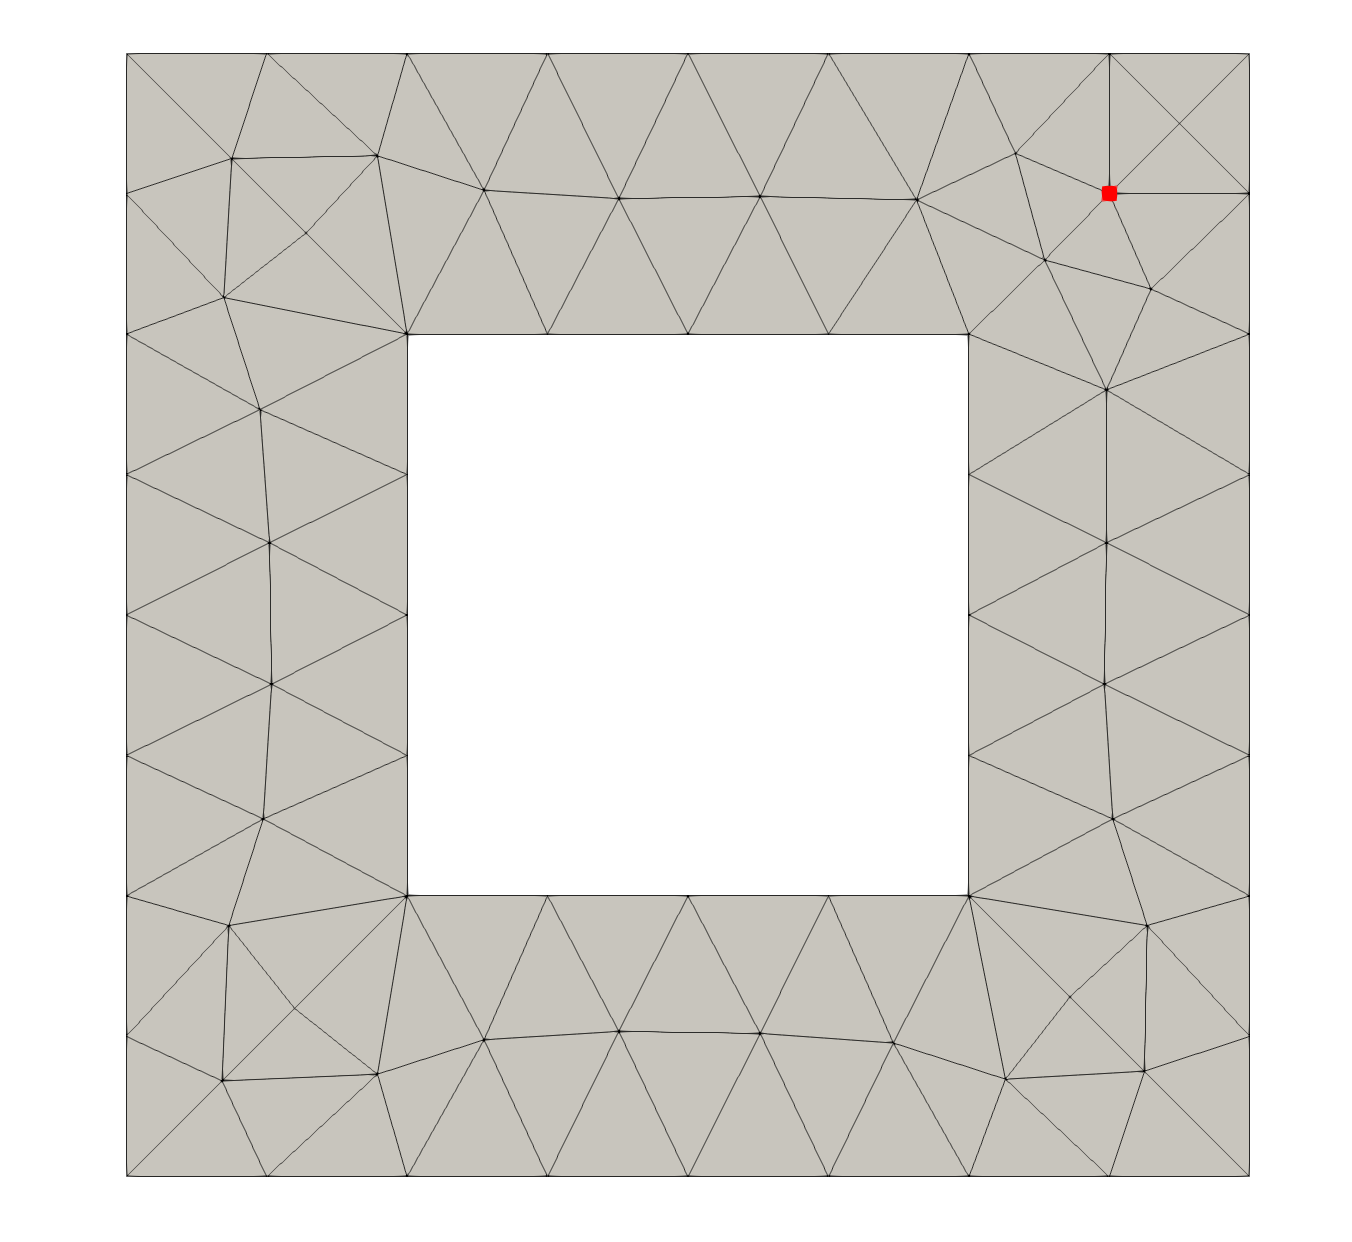
\includegraphics[width=.99\linewidth]{img/aut_squarehole_initial.png}
\end{subfigure}%
\begin{subfigure}{0.31\textwidth}
\centering
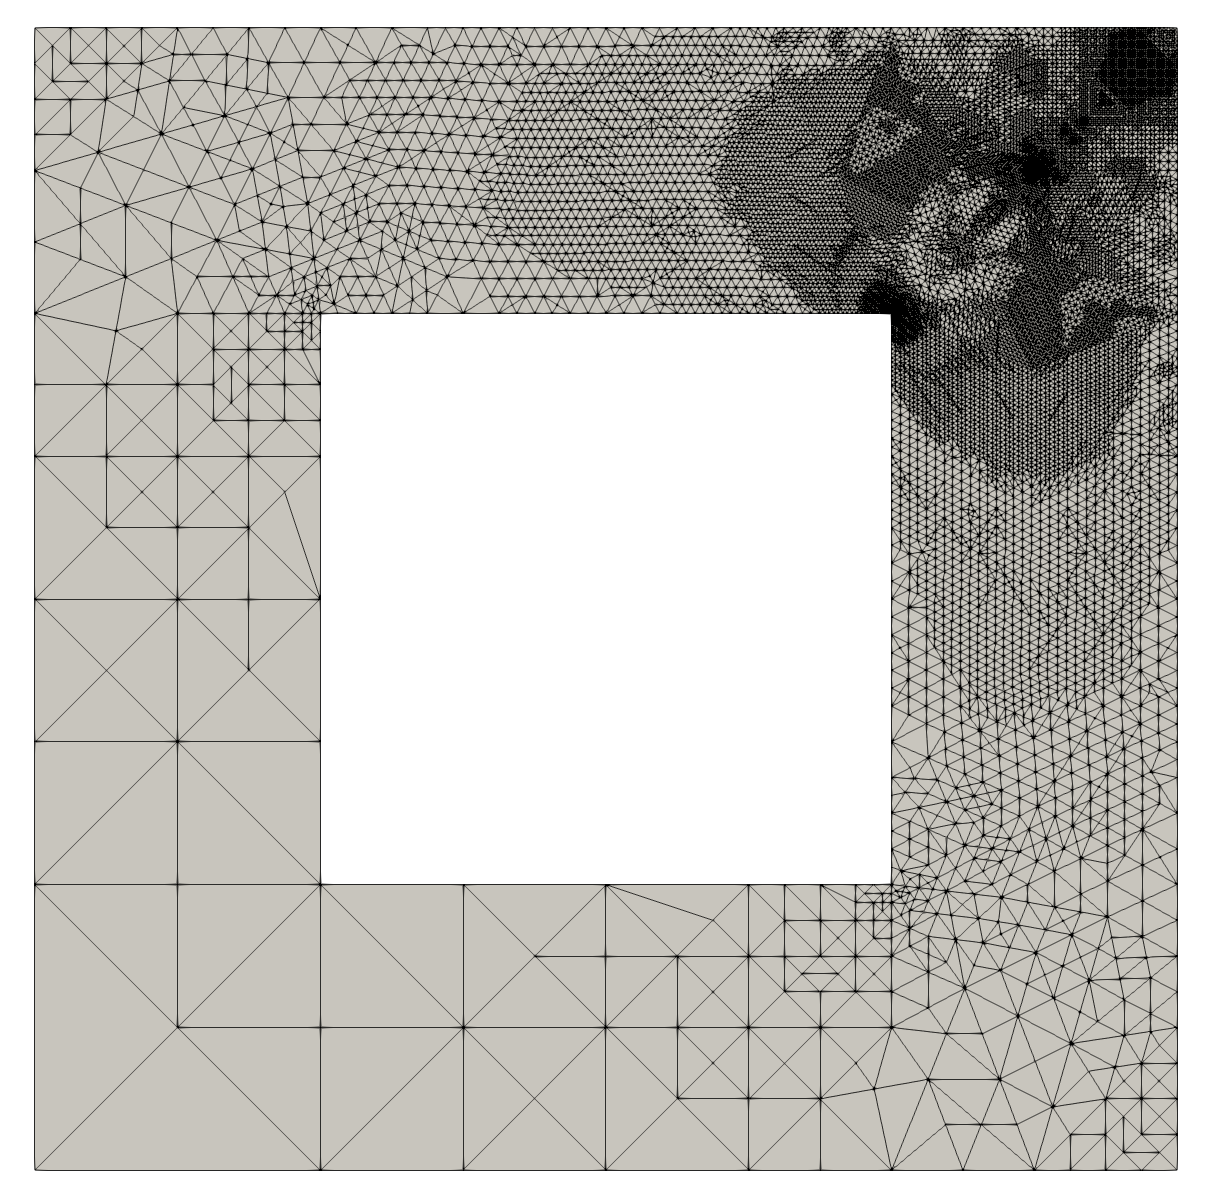
\includegraphics[width=.99\linewidth]{img/aut_squarehole_unif.png}
\end{subfigure}%
\begin{subfigure}{0.32\textwidth}
\centering
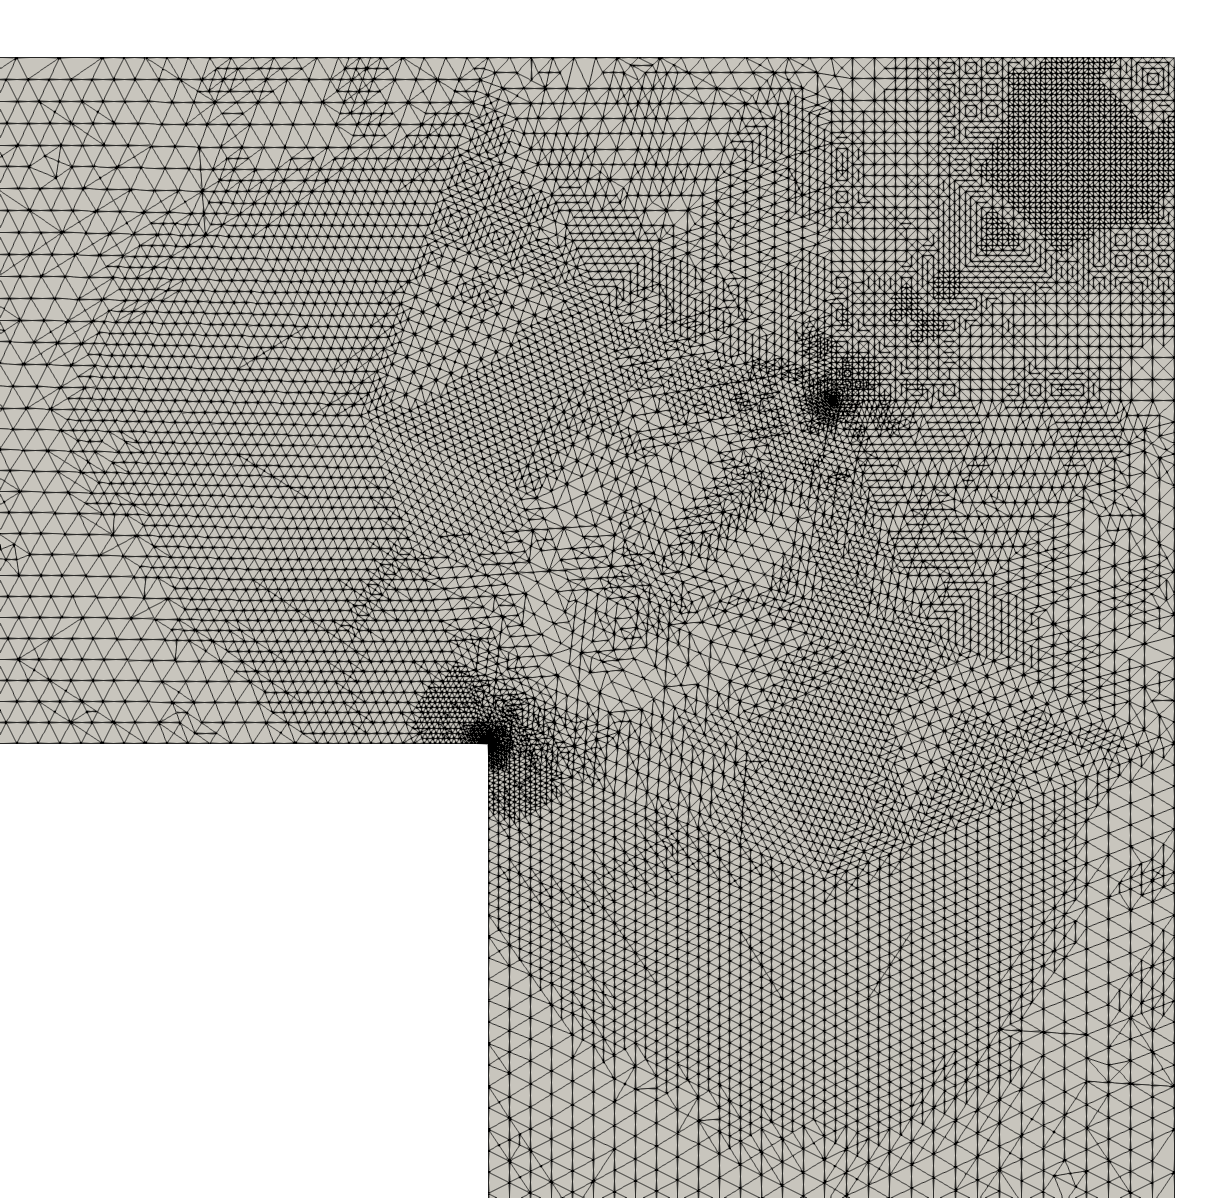
\includegraphics[width=.99\linewidth]{img/aut_squarehole_unif_close.png}
\end{subfigure}
\caption{Domain and initial mesh (left) for the Poisson's equation example
with the QoI point indicated in red, final adapted mesh (middle), and
a close up of the upper-right hand corner of the final adapted mesh (right).}
\label{fig:aut_poisson_meshes}
\end{figure}

Starting from the initial mesh shown in Figure \ref{fig:aut_poisson_meshes},
the steps:
%
\begin{gather*}
\text{Solve Primal} \rightarrow \text{Solve Adjoint} \rightarrow
\text{Estimate Error} \rightarrow \text{Adapt Mesh}
\end{gather*}
%
were performed seven times. The adaptive simulation was run using
4 MPI ranks. The mesh size field was set according to
equation \eqref{eq:aut_size_field} so that the target number of elements
is twice that of the current mesh. Figure \ref{fig:aut_poisson_meshes}
also shows the final adapted mesh resulting from this procedure. We remark
that the distribution of degrees of freedom in this mesh closely
resembles the results obtained in reference \cite{dealiistep14}.

%
%% aut_squarehole_effectivity
\begin{figure}[ht!]
\centering
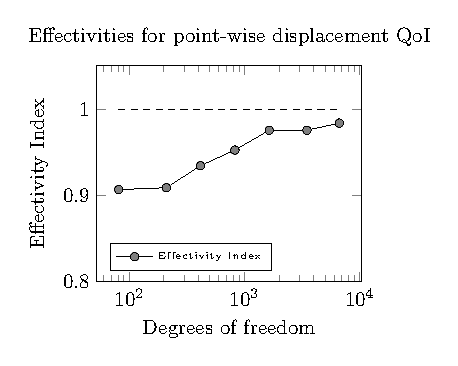
\includegraphics[width=.5\textwidth]{img/aut_squarehole_effectivity.pdf}
\caption{Effectivity indices for the adaptive Poisson's equation example.}
\label{fig:aut_squarehole_effectivity}
\end{figure}

We expect this functional to converge
at the rate $k=2$, such that the scaling factor $\alpha$ used in
the estimate \eqref{eq:aut_error_estimate} is given as
$\alpha = \frac34$. We consider the ``exact error''
$\E = J(u) - J(u^H)$ and the effectivity index
$\I = \frac{\eta}{\E}$, where $\eta$ is the estimate given by
equation \eqref{eq:aut_error_estimate}. Here we have placed quotations
around the term exact error because we have only approximated the
exact value of the QoI $J(u)$, and not truly recovered its exact value.
Figure \ref{fig:aut_squarehole_effectivity} plots the effectivity index
$\I$ versus the number of degrees of freedom in the adaptive
process. This plot demonstrates the ability of the error
estimate to recover the ``exact error'' as $H \to 0$.

%
%% aut_squarehole_error
\begin{figure}[ht!]
\centering
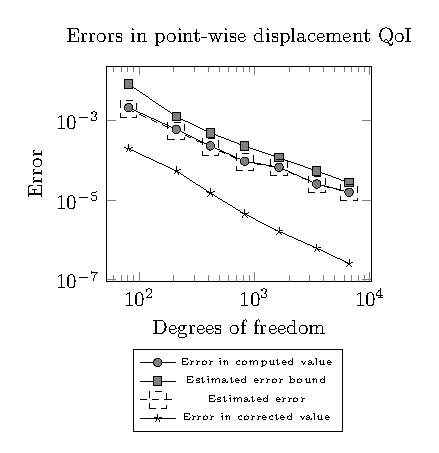
\includegraphics[width=.5\textwidth]{img/aut_squarehole_error.pdf}
\caption{Errors for the point-wise QoI for the adaptive Poisson's equation
example.}
\label{fig:aut_squarehole_error}
\end{figure}

Figure \ref{fig:aut_squarehole_error} displays the evolution of
various during the adaptive process. The ``exact error'' $\E$
and the estimated error $\eta$ are very close, as previously
demonstrated by the effectivity index $\I$. Additionally, the
approximated upper bound on the error $\hat{\eta}$ overestimates
the error, but not to a large degree. This provides some indication
that the correction indicators are effective in that they do
not drastically overestimate error. Finally, we remark that an
improved \emph{corrected} QoI functional value can be
computed as $J^*(u^H) = J(u^H) + \eta$. Figure
\ref{fig:aut_squarehole_error} demonstrates that this corrected
value is nearly an order of magnitude more accurate than
the computed functional value $J(u^H)$ during the adaptive process.

%
%% aut_squarehole_convergence
\begin{figure}[ht!]
\centering
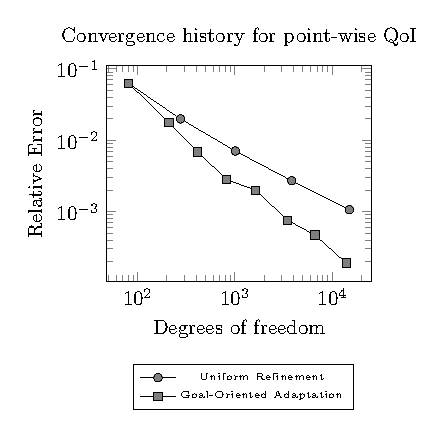
\includegraphics[width=.5\textwidth]{img/aut_squarehole_convergence.pdf}
\caption{Error convergence using uniform mesh refinement and adjoint-based
error estimation for the adaptive Poisson's equation example.}
\label{fig:aut_squarehole_convergence}
\end{figure}

Finally, Figure \ref{fig:aut_squarehole_convergence} demonstrates the
evolution of the ``exact error'' for two adaptive strategies.
The first strategy uniformly refines the mesh at each adaptive
step and the second strategy performs the adjoint-based adaptive scheme
developed in this work. We note that the error for the adjoint-based
adaptive scheme converges faster than the uniform refinement scheme.
Further, this convergence plot is consistent with the reference
\cite{dealiistep14}. 

%%% NONLINEAR ELASTICITY
\subsection{A Cell Embedded in a Matrix}

Recently, the automated approach developed in this paper was applied
to a stabilized mixed pressure-displacement finite element formulation
\cite{ramesh2005stabilized} for the governing equations of finite
deformation elasticity in a total Lagrangian setting
\cite{granzow2017adjoint} (see Chapter \ref{chap:mech}).
For two and three dimensional problems in
nonlinear elasticity, the automated approach was shown to effectively
estimate the error and provide improved error convergence rates via
adjoint-based mesh adaptation over uniform refinement.

In this section, the parallelization of a biomechanical application
presented in the reference \cite{granzow2017adjoint} is discussed. First,
the governing equations are briefly reviewed. For mixed pressure-displacement
formulations in the Goal application, the Galerkin residual is
defined as:
%
%% aut_mech_galerkin
\begin{gather}
\begin{aligned}
&\R_g(\bs{W}^H ; \bs{U}^H) := \\
&\int_{\Omega} \bs{P} : \nabla \bs{w}^H \, \text{d} \Omega +
\int_{\Omega} \left[ \frac{p^H}{\kappa} - \frac{1}{2 J}(J^2 - 1) \right] \;
q^H \, \text{d} \Omega -
\int_{\partial \Omega_h} \bs{h} \cdot \bs{w} \; \text{d} \Gamma,
\end{aligned}
\label{aut:mech_galerkin}
\end{gather}
%
and the stabilization residual is defined as:
%
%% aut_mech_stabilized
\begin{gather}
\R_{\tau}(\bs{W}^H ; \bs{U}^H) :=
\sum_{e=1}^{n_{el}} \int_{\Omega_e} \tau_e
(J \bs{F}^{-1} \bs{F}^{-T}) : (\nabla p^H \otimes \nabla q^H) \;
\text{d} \Omega.
\label{aut_mech_stabilized}
\end{gather}
%
Here, $\bs{F}$ is the deformation gradient, $J := \text{det}(\bs{F})$,
$\bs{h}$ is an applied traction over the boundary $\partial \Omega_h$,
$\bs{P} := J \bs{\sigma} \bs{F}^{-T}$ is the first Piola-Kirchhoff
stress tensor, $\bs{\sigma}$ is the Cauchy stress tensor, $n_{el}$
is the total number of elements in the mesh, and $\tau_e :=
\frac{c_0 H_e^2}{2 \mu}$ is a mesh-dependent stabilization parameter,
where $c_0$ is a non-negative stability constant, $H_e$ denotes an
element mesh size and $\mu$ denotes the bulk modulus.
The Cauchy stress tensor is defined via a neo-Hookean constitutive
relationship.  The total
solution vector is defined as $\bs{U}^H := [\bs{u}^H, p^H]$, where
$\bs{u}^H$ corresponds to displacements and $p^H$ corresponds to
pressures. Similarly, the total weighting vector is defined as
$\bs{W}^H := [\bs{w}^H, q^H]$, where $\bs{w}^H$ denotes a weighting
function corresponding to displacements and $q^H$ is a weighting
function corresponding to pressures. For a complete
exposition, we refer the reader to Chapter \ref{chap:mech}.

%
%% aut_glial_geom
\begin{figure}[ht!]
\centering
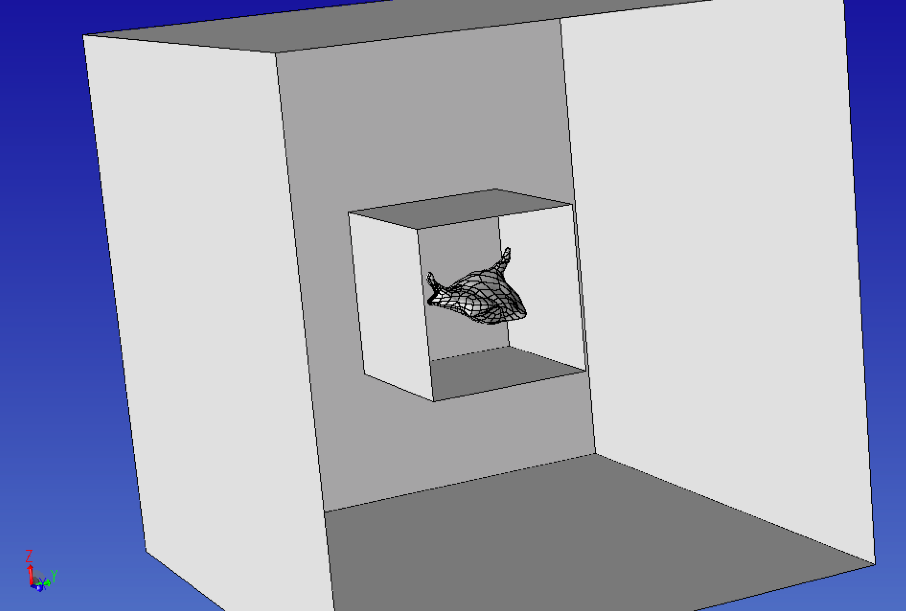
\includegraphics[width=.5\linewidth]{img/aut_glial_geom.png}
\caption{Domains for the microglial cell example.}
\label{fig:aut_glial_geom}
\end{figure}

We focus on a microglial cell with dimensions of about
$20 \mu m \times 20 \mu m \times 20 \mu m$ embedded in an extracellular
matrix of dimension $100 \mu \times 100 \mu m \times 100 \mu m$.
The QoI is chosen to be a local average displacement
$J(\bs{U}) = \int_{\Omega_0} \frac13 (u_x + u_y + u_z) \, \text{d} \Omega$,
defined over a box $\Omega_0$ with dimensions
$30 \mu m \times 30 \mu m \times 30 \mu m$
that bounds the microglial cell. Figure \ref{fig:aut_glial_geom} shows
the geometry defining the microglial cell, the bounding box
$\Omega_0$, and the extracellular matrix. The shear modulus
is defined as $\mu = 600$ Pa and Poisson's ratio is set to be
$\nu = 0.4999$.

To drive the problem, traction boundary conditions are imposed along
the surface of the microglial cell. The magnitude of the applied
traction $\bs{h}$ is defined to be 10 times the distance to the
center of the cell and its direction points inward towards the
cell center. This traction is consistent with observed physical
behavior \cite{dong2017recovery}. Displacements $u_x = 0$,
$u_y=0$, and $u_z=0$ are applied to the faces with constant
minimum $x$-coordinate value, constant minimum $y$-coordinate
value, and constant minimum $z$-coordinate value, respectively,
to constrain rigid body rotations and translations.

%
%% aut_glial_meshes
\begin{figure}[ht!]
\centering
\begin{subfigure}{.33\textwidth}
\centering
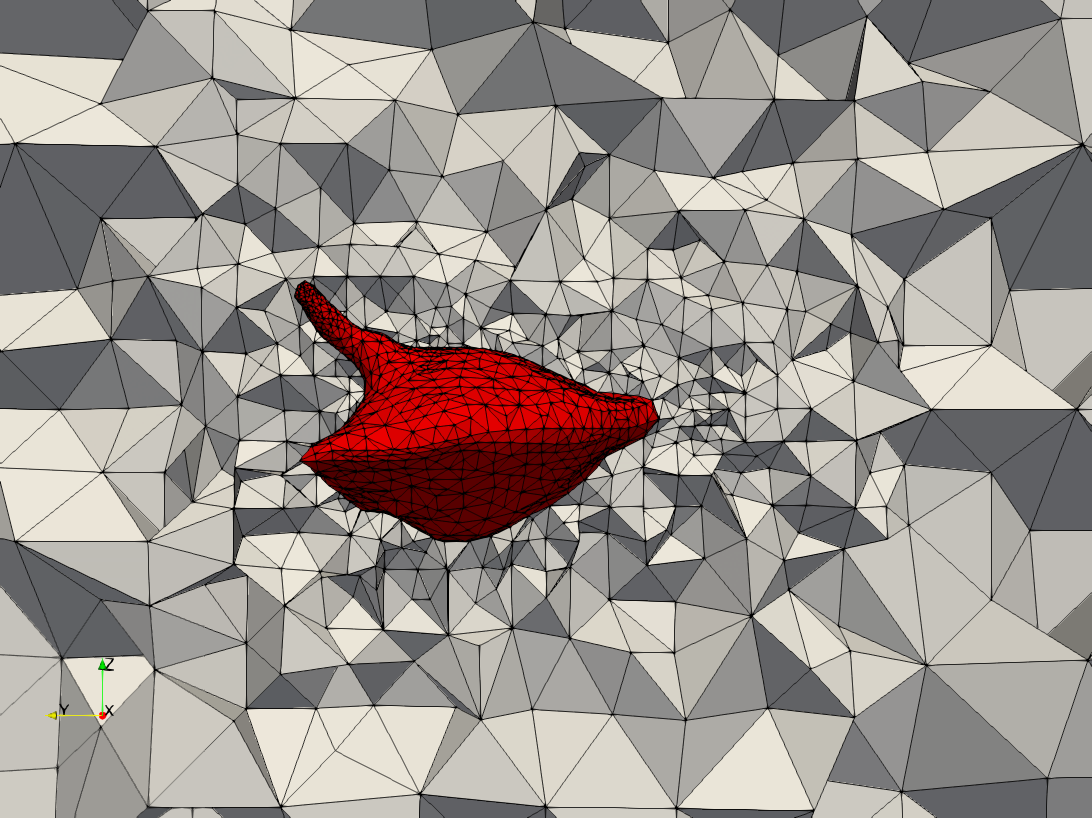
\includegraphics[width=.99\linewidth]{img/aut_glial_mesh0.png}
\end{subfigure}%
\begin{subfigure}{0.33\textwidth}
\centering
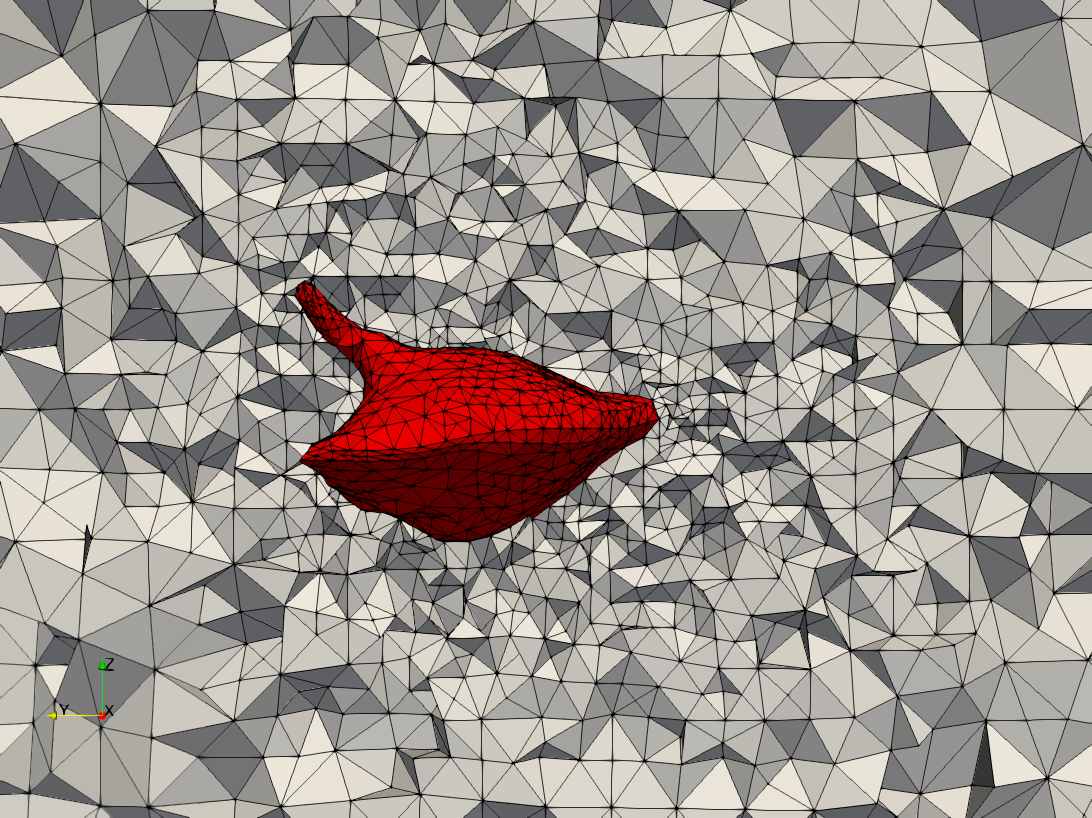
\includegraphics[width=.99\linewidth]{img/aut_glial_mesh5.png}
\end{subfigure}%
\begin{subfigure}{0.33\textwidth}
\centering
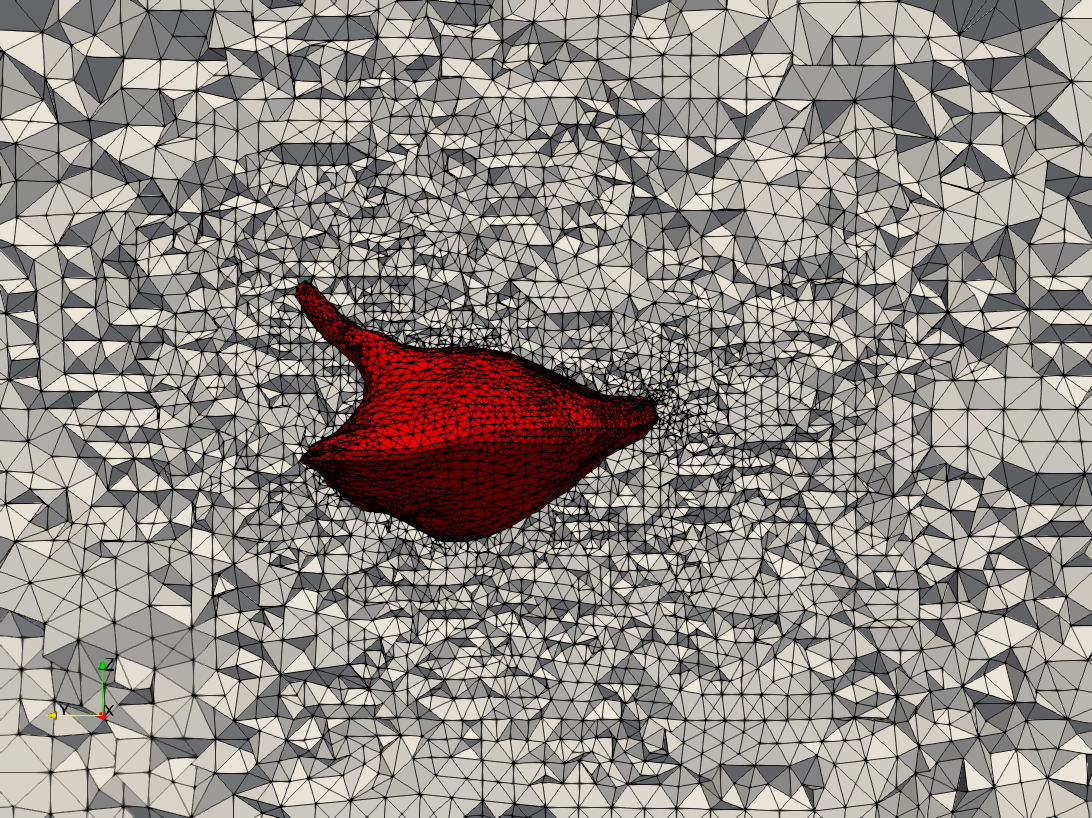
\includegraphics[width=.99\linewidth]{img/aut_glial_mesh10.png}
\end{subfigure}
\caption{A close-up of the initial mesh (left) the mesh after
5 adaptive iterations (center) and the final adapted mesh (right)
for the microglial cell example}
\label{fig:aut_glial_meshes}
\end{figure}

Figure \ref{fig:aut_glial_meshes} demonstrates an initial mesh,
which contains around $30,000$ degrees of freedom. From this initial
mesh, the steps
%
\begin{gather*}
\text{Solve primal PDE} \rightarrow
\text{Solve adjoint PDE} \rightarrow
\text{Localize error} \rightarrow
\text{Adapt mesh}
\end{gather*}
%
were successively performed $10$ times. During the adapt stage,
the mesh size field was set such that desired number of elements
$N$ in the output mesh is $1.5$ times the number of elements
in the previous mesh, according to equation \eqref{eq:aut_size_field}.
Figure \ref{fig:aut_glial_meshes} additionally demonstrates the adapted
meshes obtained at the fifth and final adaptive iteration.
In particular, both \emph{coarsening} and \emph{refinement} is performed
during the adaptive iterations.

\begin{figure}[ht!]
\centering
\begin{subfigure}{.5\textwidth}
\centering
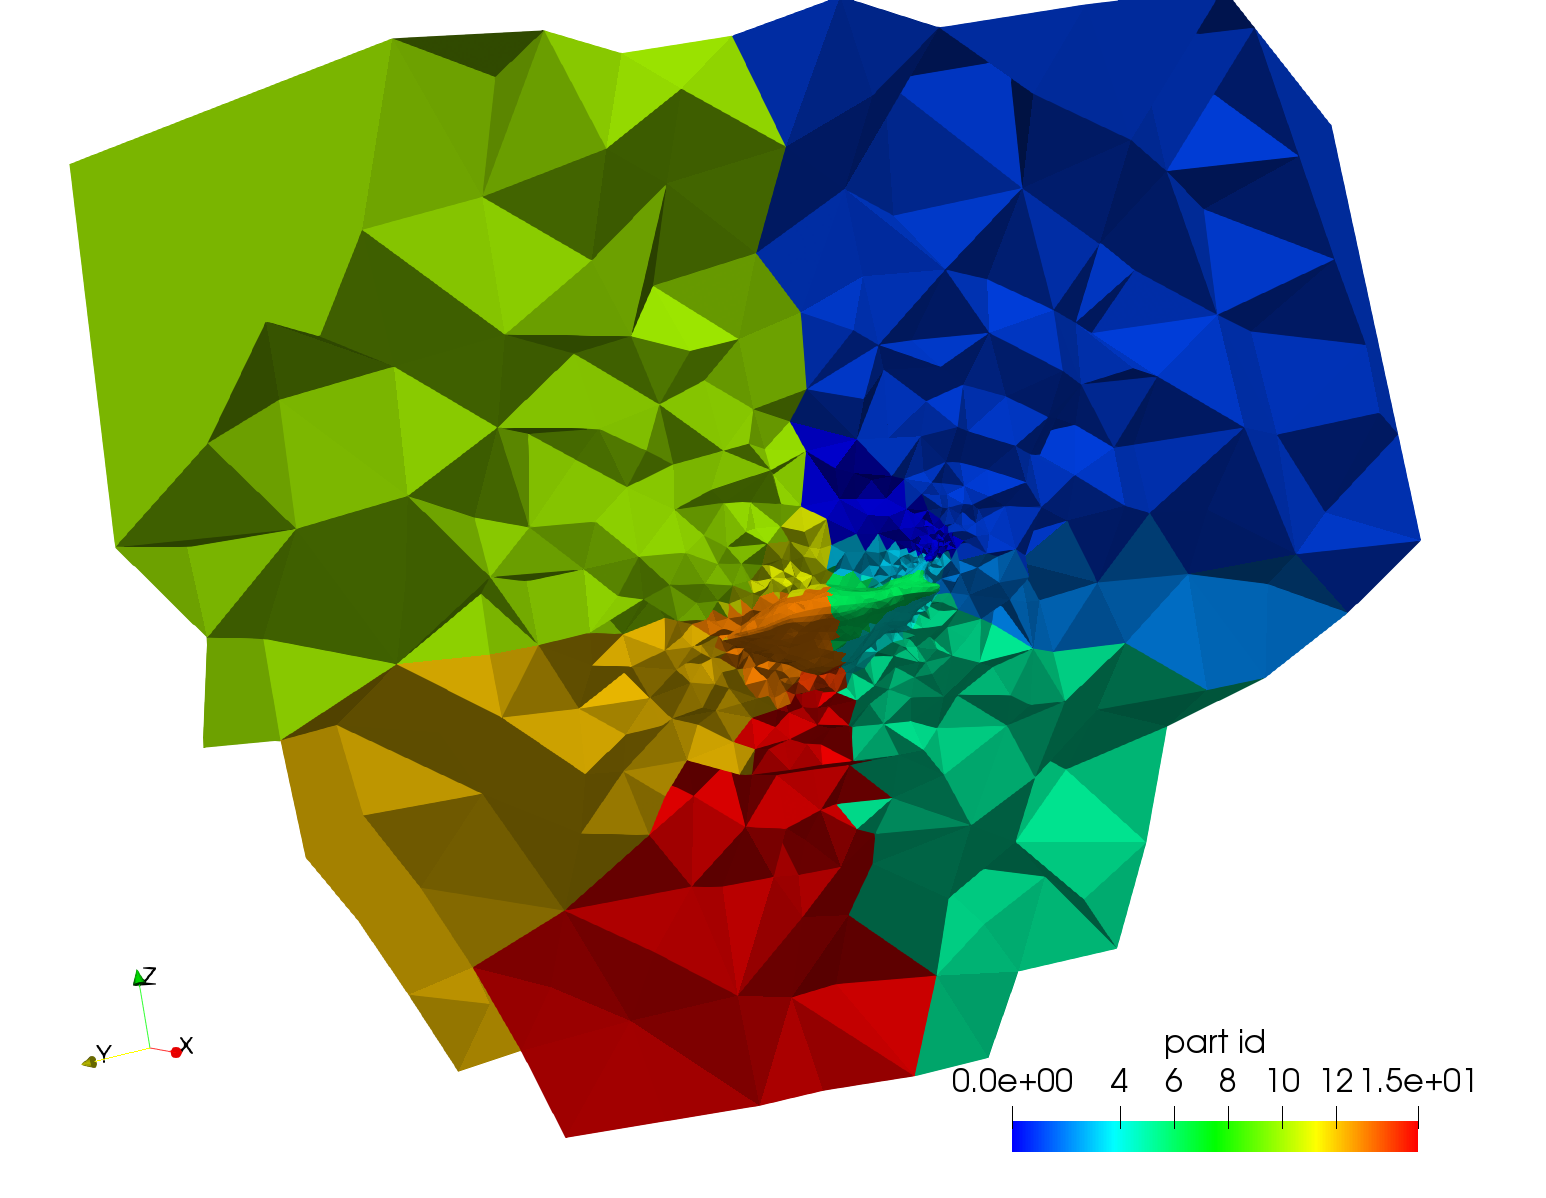
\includegraphics[width=.99\linewidth]{img/aut_glial_initial_parts.png}
\end{subfigure}%
\begin{subfigure}{0.5\textwidth}
\centering
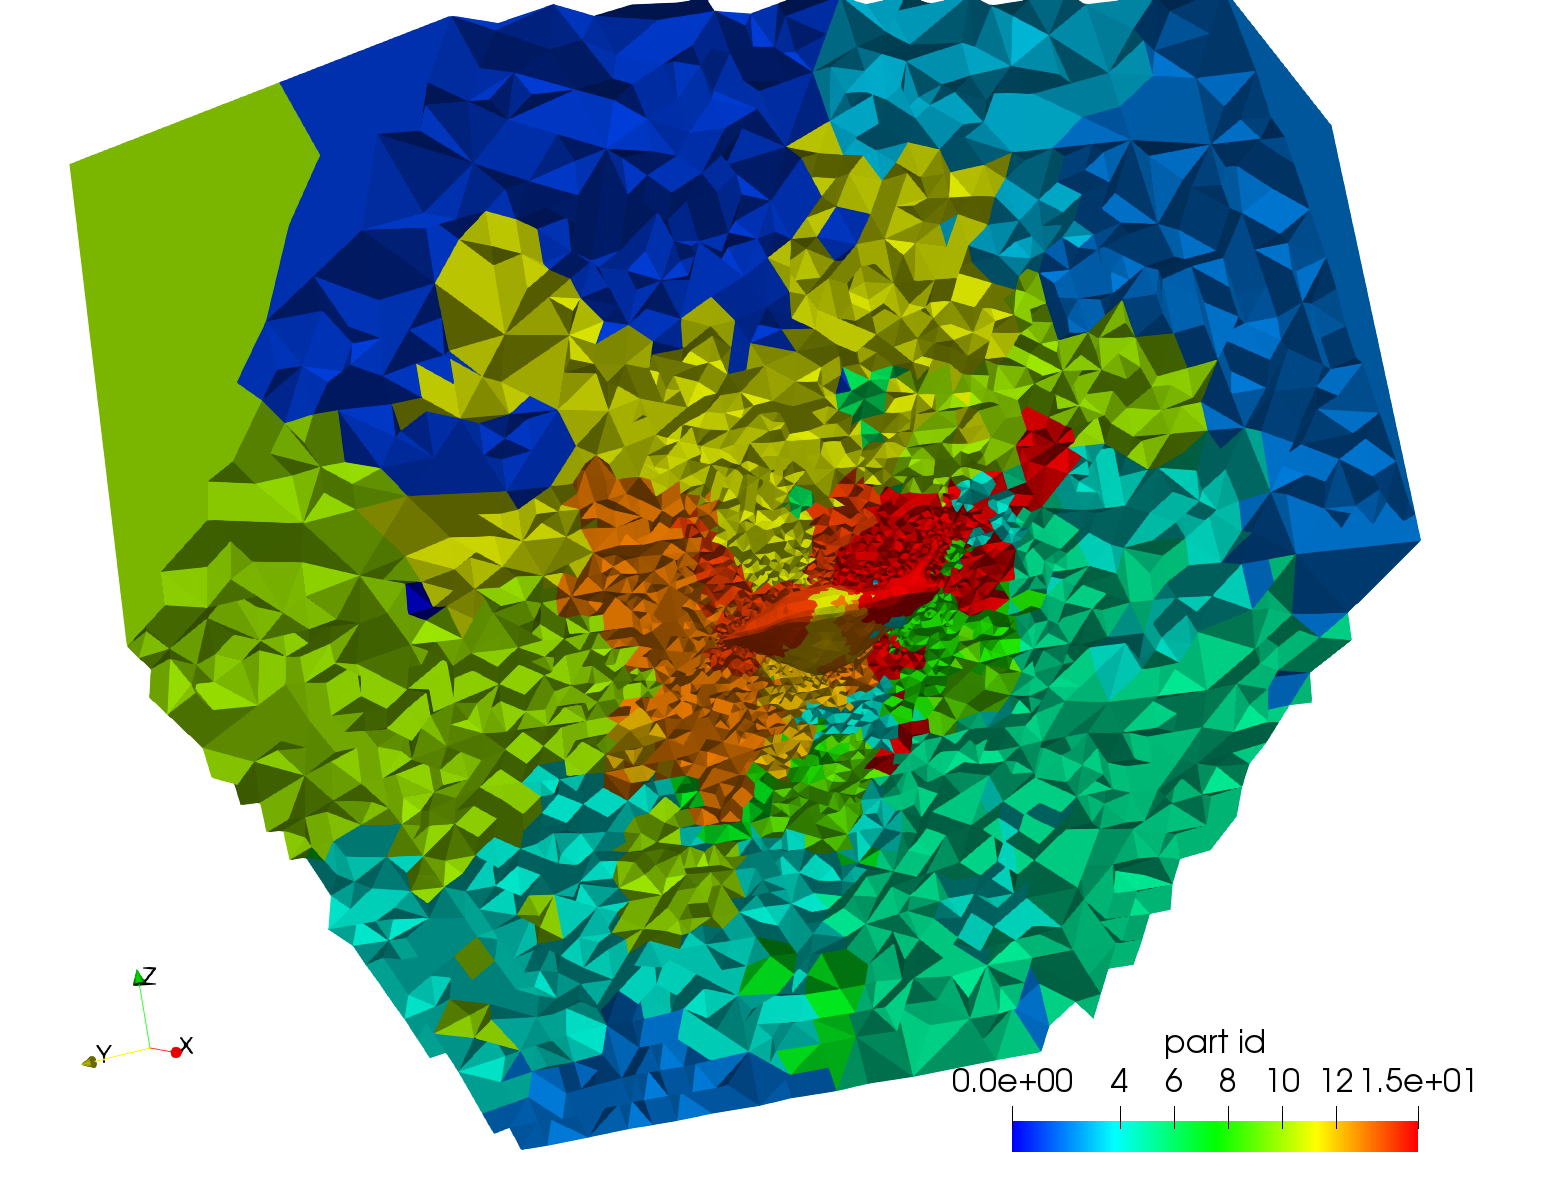
\includegraphics[width=.99\linewidth]{img/aut_glial_final_parts.png}
\end{subfigure}
\caption{The parallel mesh partitioning for the initial mesh (left)
and the final adapted mesh (right) for the microglial cell example}
\label{fig:aut_glial_parts}
\end{figure}

The problem was run using 16 MPI ranks. Figure \ref{fig:aut_glial_parts}
demonstrates the parallel partitioning for the initial mesh and for
the final adapted mesh obtained after 10 adjoint-based adaptive
iterations. To ensure partitioning quality, ParMA was
utilized to guarantee the imbalance of vertices and elements
across parallel partitions is no greater than $5\%$.

\begin{figure}[ht!]
\centering
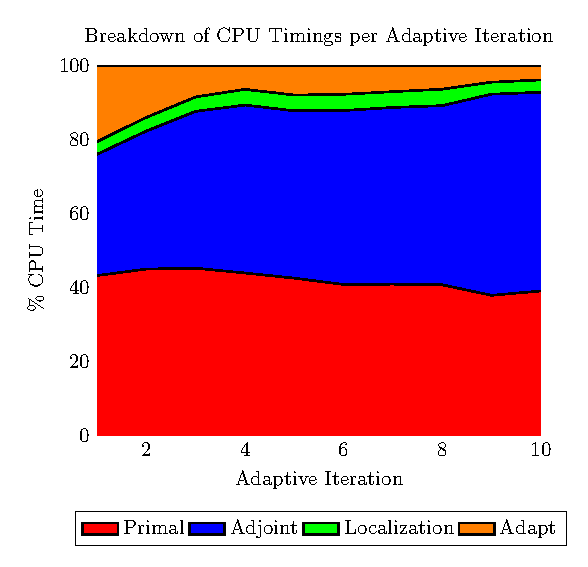
\includegraphics[width=0.4\linewidth]{img/aut_glial_timings.pdf}
\caption{Breakdown of the CPU time spent for each portion of
the adaptive process for the microglial cell example}
\label{fig:aut_glial_timings}
\end{figure}

Figure \ref{fig:aut_glial_timings} presents a breakdown of the
total percentange of CPU time spent on each step in the
adaptive analysis. For every adaptative iteration, the error
localization \eqref{eq:aut_stabilized_localization} takes only
a small percentage of the total CPU time, as it essentially amounts
to an evaluation of the residual vector the fine space. More
interestingly, mesh adaptation initially accounts for about
20 percent of the total CPU time but decreases as the adaptive
simulation progresses. This is explained by the fact that the initial
adaptive iteration requires more work to optimally distribute
the degrees of freedom for the functional QoI as compared to
subsequent adaptive iterations. In addition to refinement
and coarsening operations, the mesh adaptation step also
performs \emph{shape correction} to ensure elements are not
too heavily skewed \cite{li20053d}. Finally, we note that the
adjoint problem accounts for roughly 40 to 50 percent of the CPU time
over the course of the adaptive simulation. While process of
adjoint-based error estimation is not cheap for this example,
we provide two justifying remarks. First, this problem required only
3 to 4 Newton iterations for each primal solve. For constitutive
models with higher degrees of nonlinearity or for problems loaded to
higher strains, it is not uncommon for Newton's method to converge
in 7 to 10 iterations. In these scenarios, the relative cost of
adjoint-based error estimation is not as extreme.
Second, for this computational price, we have
achieved very accurate error estimates as shown in
Chapter \ref{chap:mech}.

%%% ELASTOPLASTICITY IN AN ARRAY OF SOLDER BALLS
\subsection{Elastoplasticity in an Array of Solder Joints}

In this section, we investigate the utility of adjoint-based mesh
adaptation for a thermomechanical analysis of an array of solder
joints used in microelectronics fabrication. We consider a
$6 \times 6$ array of solder joints sandwiched between two materials
with distinct thermomechanical properties
to model a portion of the process of `flip-chip'
manufacturing \cite{bloomfield2017component}. The full geometry
is shown in Figure \ref{fig:aut_solder_geom}. We consider
an elastoplastic constitutive model with a von-Mises yield
surface and linear isotropic hardening, as given by
Simo and Hughes \cite{simo2006computational} with a temperature
correction for the stress tensor \cite{li2017simulation}. The top
slab, solder joints, and bottom slab are modeled with the
distinct material properties given in reference
\cite{bloomfield2017component}.

To drive the problem, the entirety of the domain is cooled
from a reference temperature $T_{ref} = 393K$ to a
resting temperature of $T_{f} = 318K$ in a single load
step. The faces with minimum $x$, $y$, and $z$ coordinate
values were constrained to have zero displacements in
the $x$, $y$, and $z$ directions, respectively. As a
QoI, we consider the average von-Mises stress given by
equation \eqref{eq:aut_avg_vm_qoi} over three solder joints
shown in yellow in Figure \ref{fig:aut_solder_geom}.

\begin{figure}[ht!]
\centering
\begin{subfigure}{.5\textwidth}
\centering
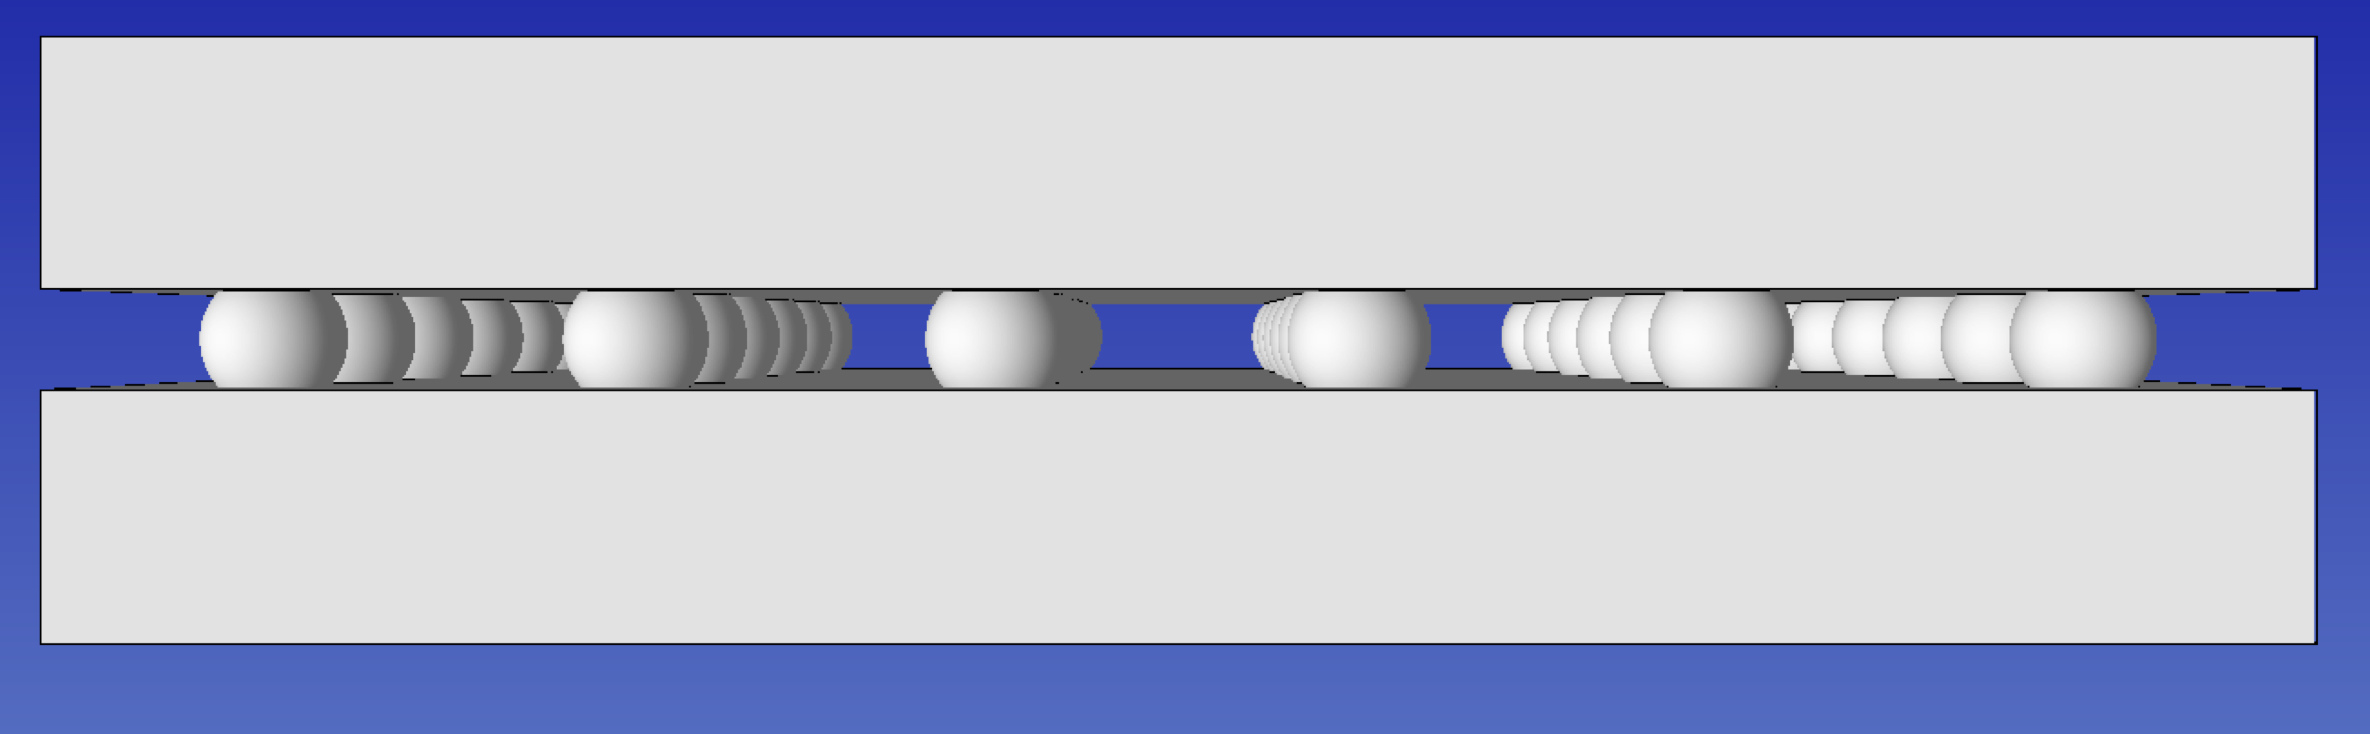
\includegraphics[width=.99\linewidth]{img/aut_solder_geom.png}
\end{subfigure}%
\begin{subfigure}{0.5\textwidth}
\centering
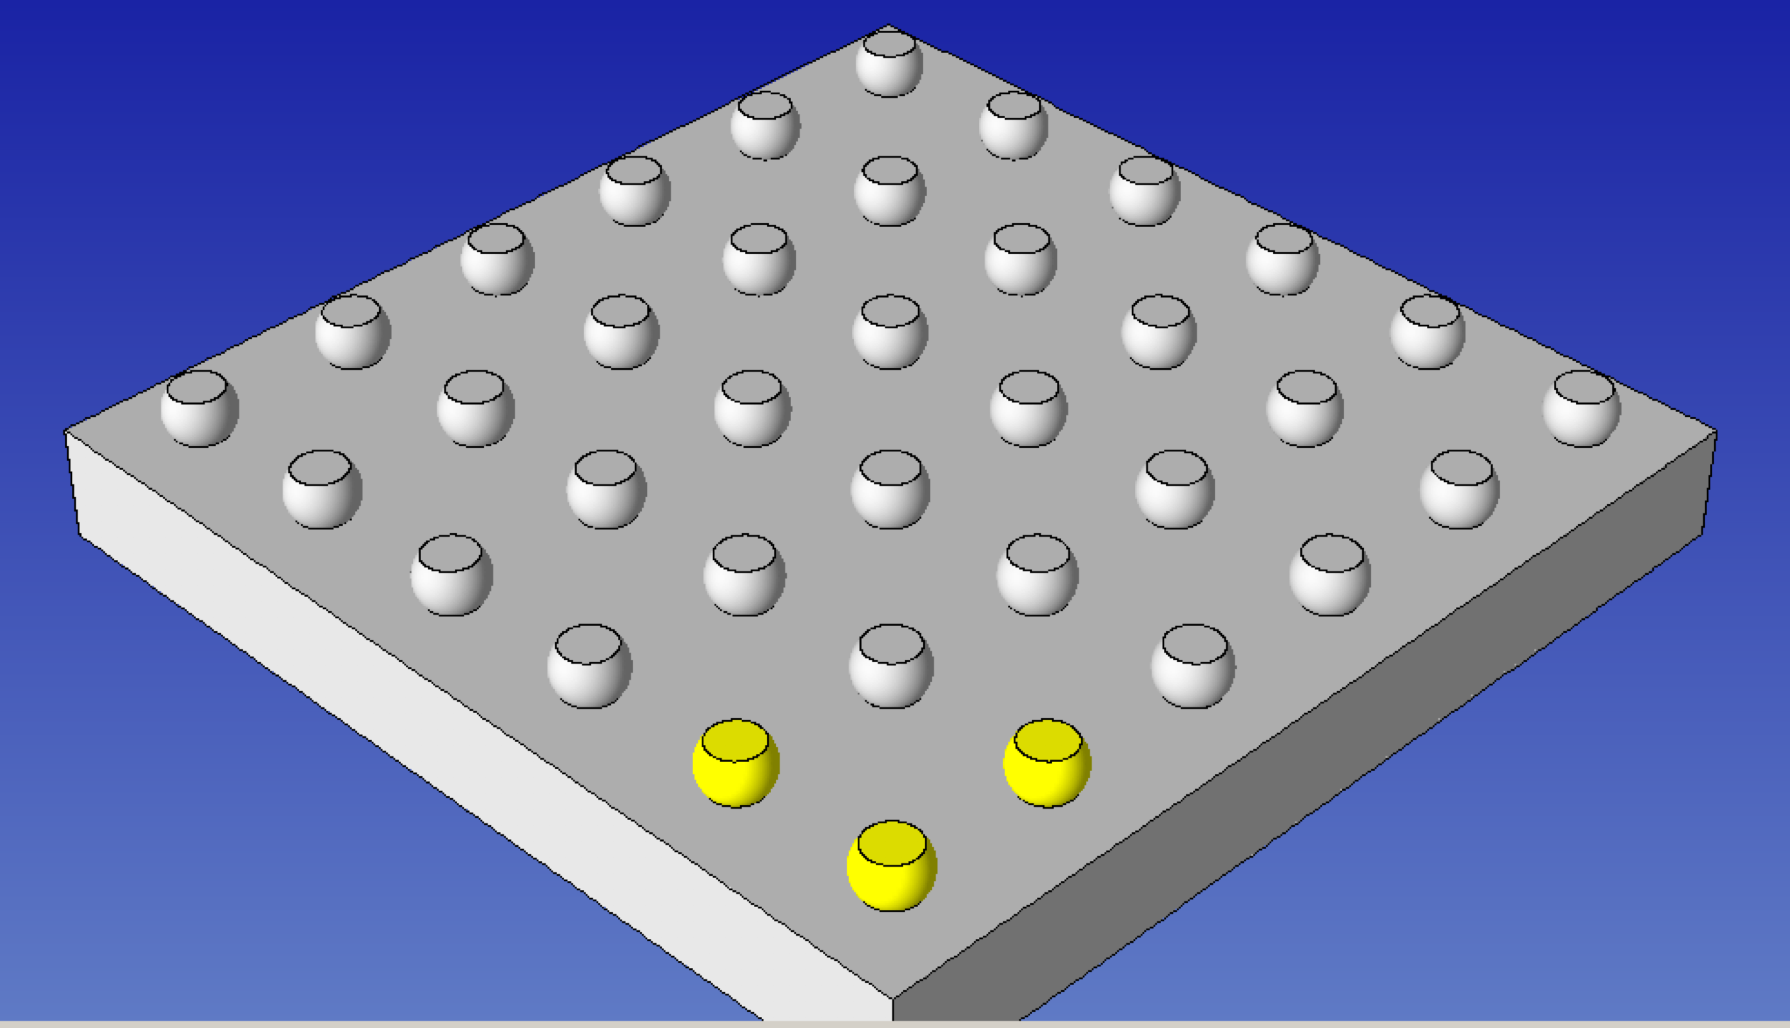
\includegraphics[width=.99\linewidth]{img/aut_solder_qoi_geom.png}
\end{subfigure}
\caption{The solder joint array geometry (left) and the
geometric specification of the average von-Mises QoI
(right).}
\label{fig:aut_solder_geom}
\end{figure}

The primal problem was solved on a sequence of uniformly refined
meshes, starting with an initial mesh with about 1 million
elements distributed over 16 MPI ranks, and finalizing with a
mesh with over half a billion elements distributed over
8192 MPI ranks. For each solve, the work load for each mesh
part (MPI rank) was held constant at approximately
$70,000$ elements. Figure \ref{fig:aut_weak_scaling}
demonstrates weak scaling timing results for various aspects
of the primal solve. In particular, we remark that the
assembly of the residual vector and Jacobian matrix scale
well as the number of MPI ranks increases. The preconditioning
routine shows a slight increase in time as the number of
MPI ranks increases, but this increase is not drastic.
The time to solve the linear system, however, does not scale
optimally. Improvements to parallel performance could likely
be made by more finely tuning the preconditioning and linear
solver routines for the specific problem, but this is outside
the scope of the present work.

\begin{figure}[ht!]
\centering
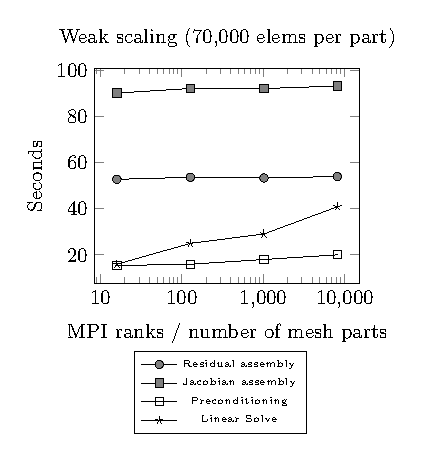
\includegraphics[width=0.5\linewidth]{img/aut_weak_scaling.pdf}
\caption{Weak scaling for the Goal application.}
\label{fig:aut_weak_scaling}
\end{figure}

The approximate QoI, $J^H(\bs{u}^H)$, was computed at each
primal solve. Using the QoI evaluations from the finest three meshes,
we performed Richardson extrapolation \cite{richardson1911approximate}
to obtain a more accurate representation of the QoI.
This value was given as $J(u) = 328.9$. We consider the extrapolated
value to be the ``true'' QoI value and measure errors with respect
to it. The expected convergence rate of the QoI is $k=1$, which is
confirmed by the Richardson extrapolation procedure.

\begin{figure}[ht!]
\centering
\begin{subfigure}{.33\textwidth}
\centering
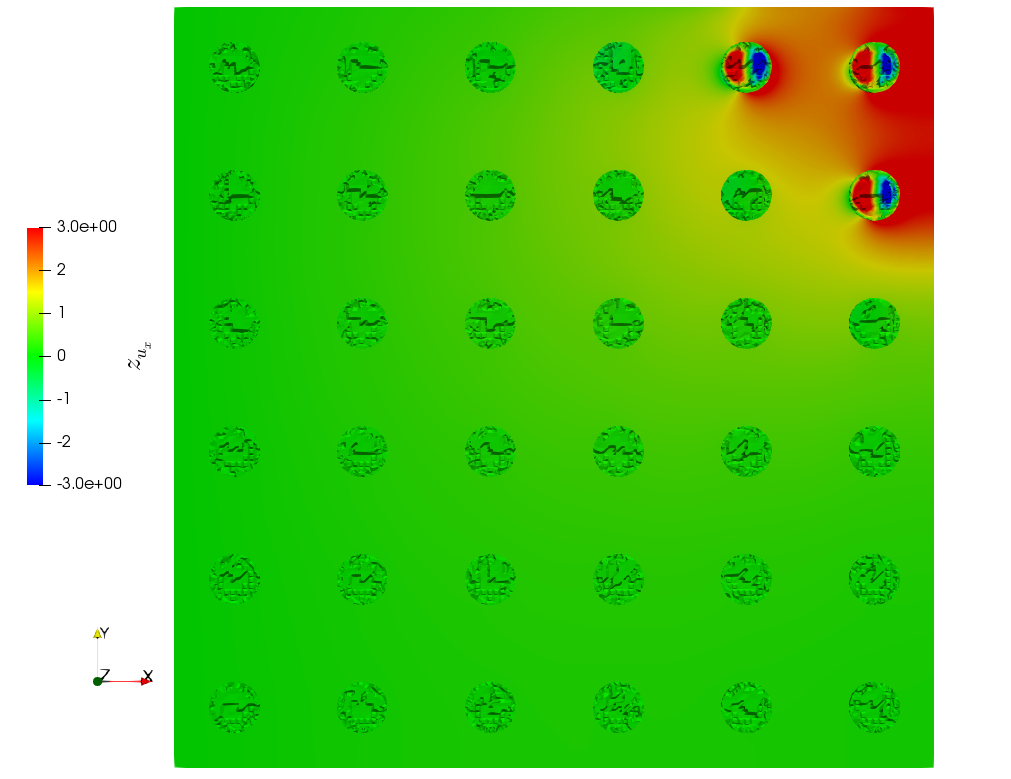
\includegraphics[width=.99\linewidth]{img/aut_solder_zux.png}
\end{subfigure}%
\begin{subfigure}{0.33\textwidth}
\centering
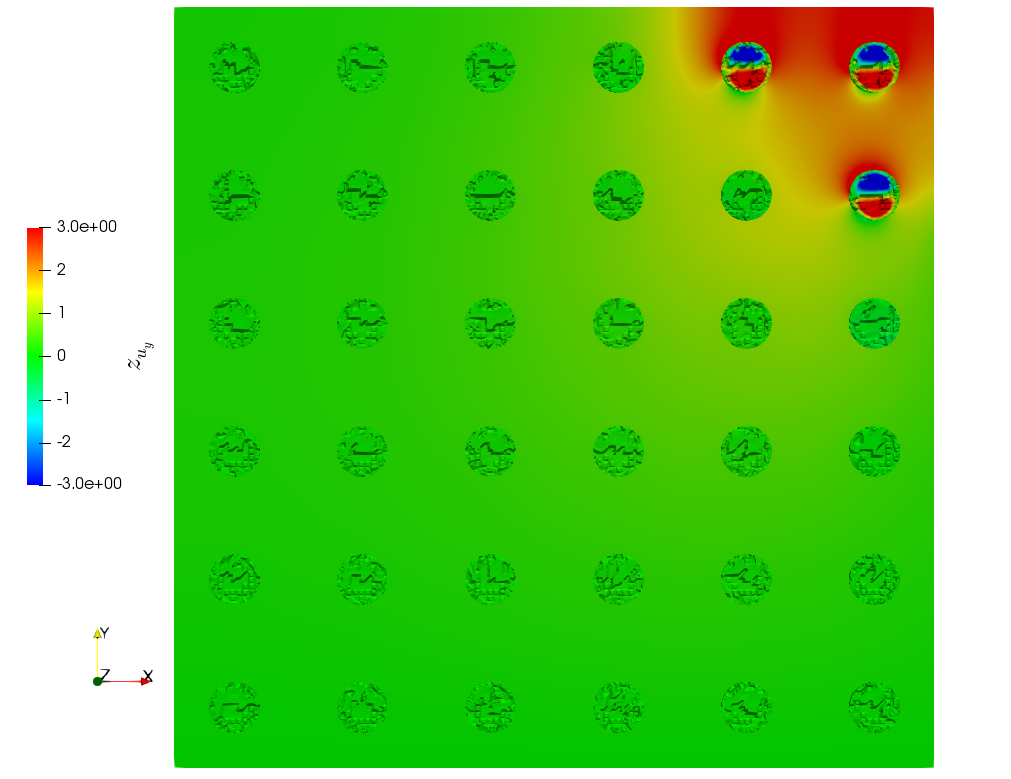
\includegraphics[width=.99\linewidth]{img/aut_solder_zuy.png}
\end{subfigure}%
\begin{subfigure}{0.33\textwidth}
\centering
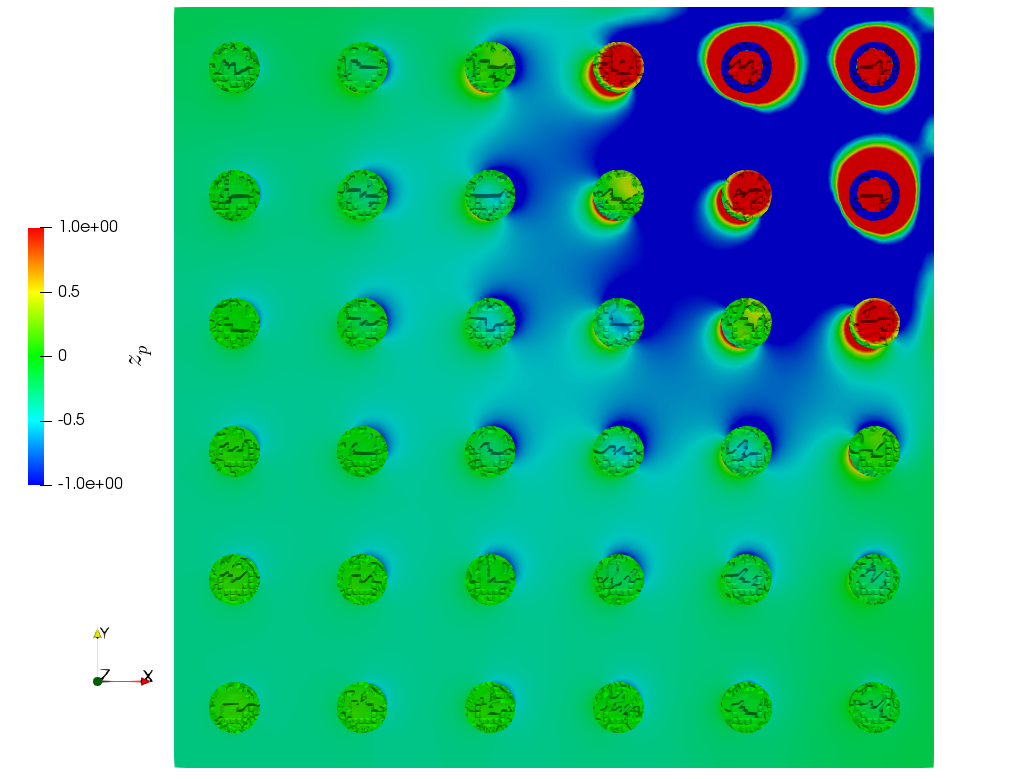
\includegraphics[width=.99\linewidth]{img/aut_solder_zp.png}
\end{subfigure}
\caption{The $x$-component of the adjoint displacement solution
(left), the $y$-component of the adjoint displacement solution
(center), and the pressure component of the adjoint solution
(right).}
\label{fig:aut_solder_adjoint}
\end{figure}

From the same initial mesh used in the weak scaling study,
we iteratively performed the steps:
%
\begin{gather*}
\text{Solve Primal} \rightarrow \text{Solve Adjoint} \rightarrow
\text{Estimate Error} \rightarrow \text{Adapt Mesh}
\end{gather*}
%
with a restart after each mesh adaptation using $128$,
$256$, and $512$ MPI ranks, such that the output number
of elements $N$ in the adapted mesh was targeted to be
$1$ million, $2$ million, and $4$ million elements,
respectively. Figure \ref{fig:aut_solder_adjoint} shows
different components of the adjoint solution obtained
during the adjoint-based adaptive process.
Figure \ref{fig:aut_solder_error} shows
the spatial distribution of the error for the given
QoI as computed by the adjoint-based error estimation process.
Unsurprisingly, the majority of the error is localized to the
area which geometrically defines the QoI. However, there are
also contributions to the error from nearby solder joints that
decrease as the distance from the 3 QoI solder joints
increases. These additional contributions to the error
are mostly gathered at the interface between solder
joints and the underlying material slab, where von-Mises
stress concentrations exist.

\begin{figure}[ht!]
\centering
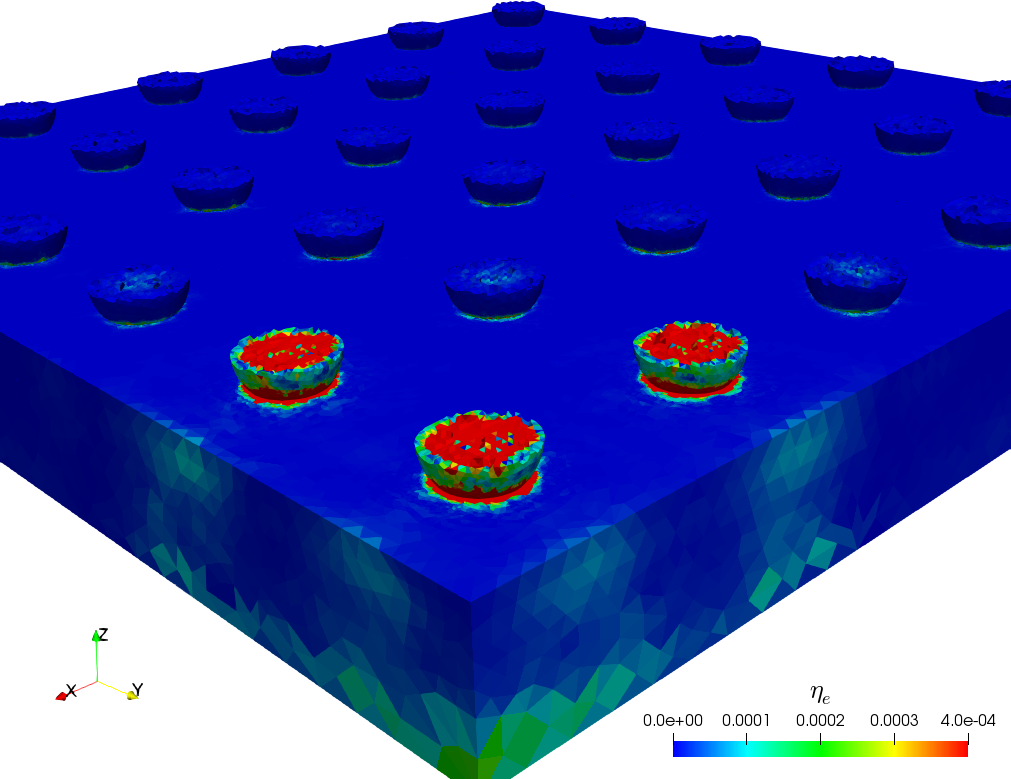
\includegraphics[width=.5\linewidth]{img/aut_solder_error.png}
\caption{The spatial distribution of errors as computed by
adjoint-based error estimation for the solder joint array.}
\label{fig:aut_solder_error}
\end{figure}

Figures \ref{fig:aut_solder_mesh} and \ref{fig:aut_solder_mesh2}
demonstrate the intial mesh used for the solder joint problem
and the final adapted mesh obtained via adjoint-based adaptation.
These figures clearly demonstrate that the 3 solder joints
that define the QoI sub-domain are heavily refined, as expected.
Additionally, notice that Figure \ref{fig:aut_solder_mesh}
demonstrates that there is refinement at the left-most solder joint,
which is not included in the geometric definition of the QoI.
The adjoint-based error estimation procedure indicates that
mesh must be refined in additional areas to accurately assess
the QoI.

\begin{figure}[ht!]
\centering
\begin{subfigure}{.5\textwidth}
\centering
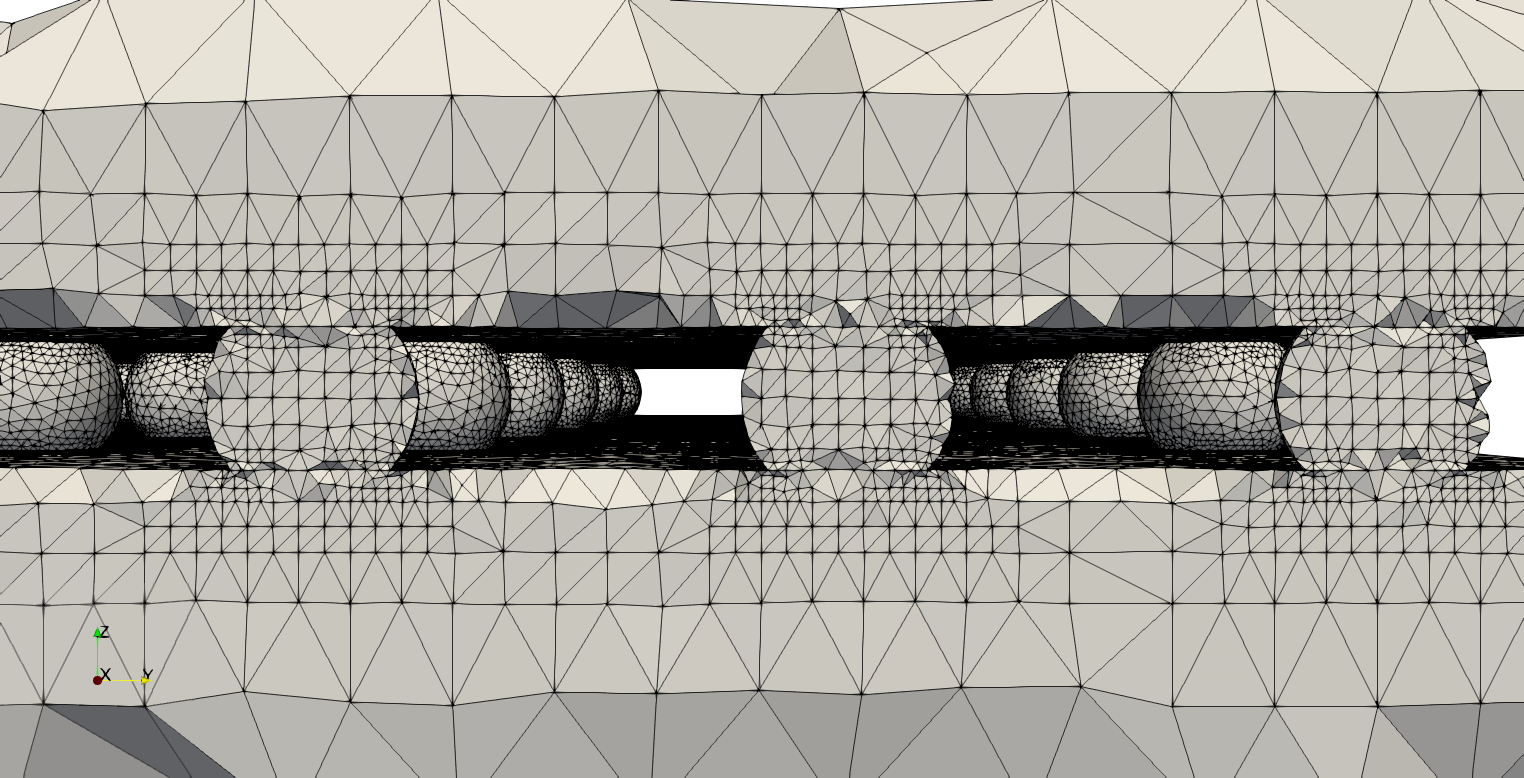
\includegraphics[width=.99\linewidth]{img/aut_solder_mesh_initial.png}
\end{subfigure}%
\begin{subfigure}{0.5\textwidth}
\centering
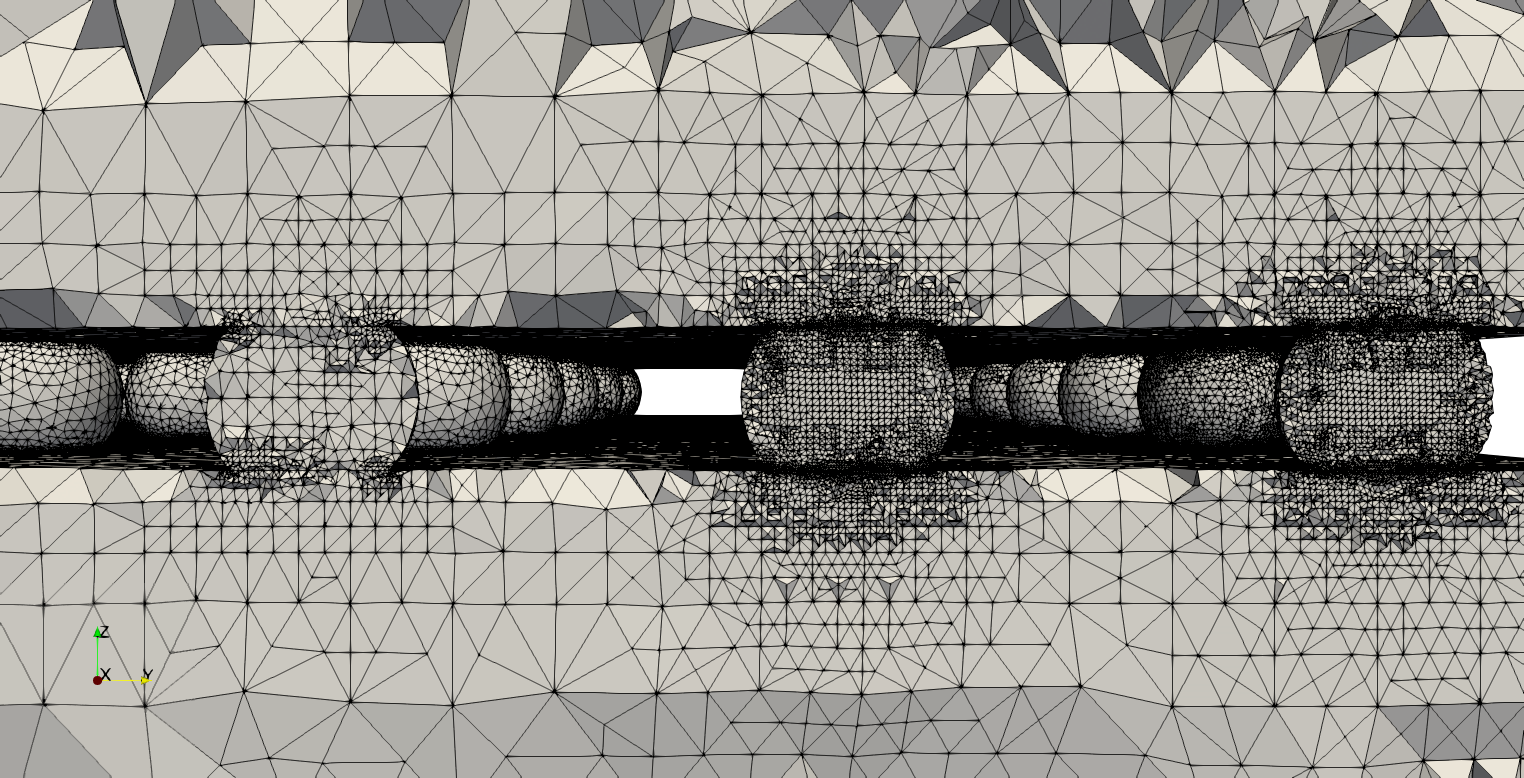
\includegraphics[width=.99\linewidth]{img/aut_solder_mesh_final.png}
\end{subfigure}%
\caption{Cross-sectional view of the initial mesh for the solder joint
geometry (left) and the final adapted mesh (right).}
\label{fig:aut_solder_mesh}
\end{figure}

\begin{figure}[ht!]
\centering
\begin{subfigure}{.5\textwidth}
\centering
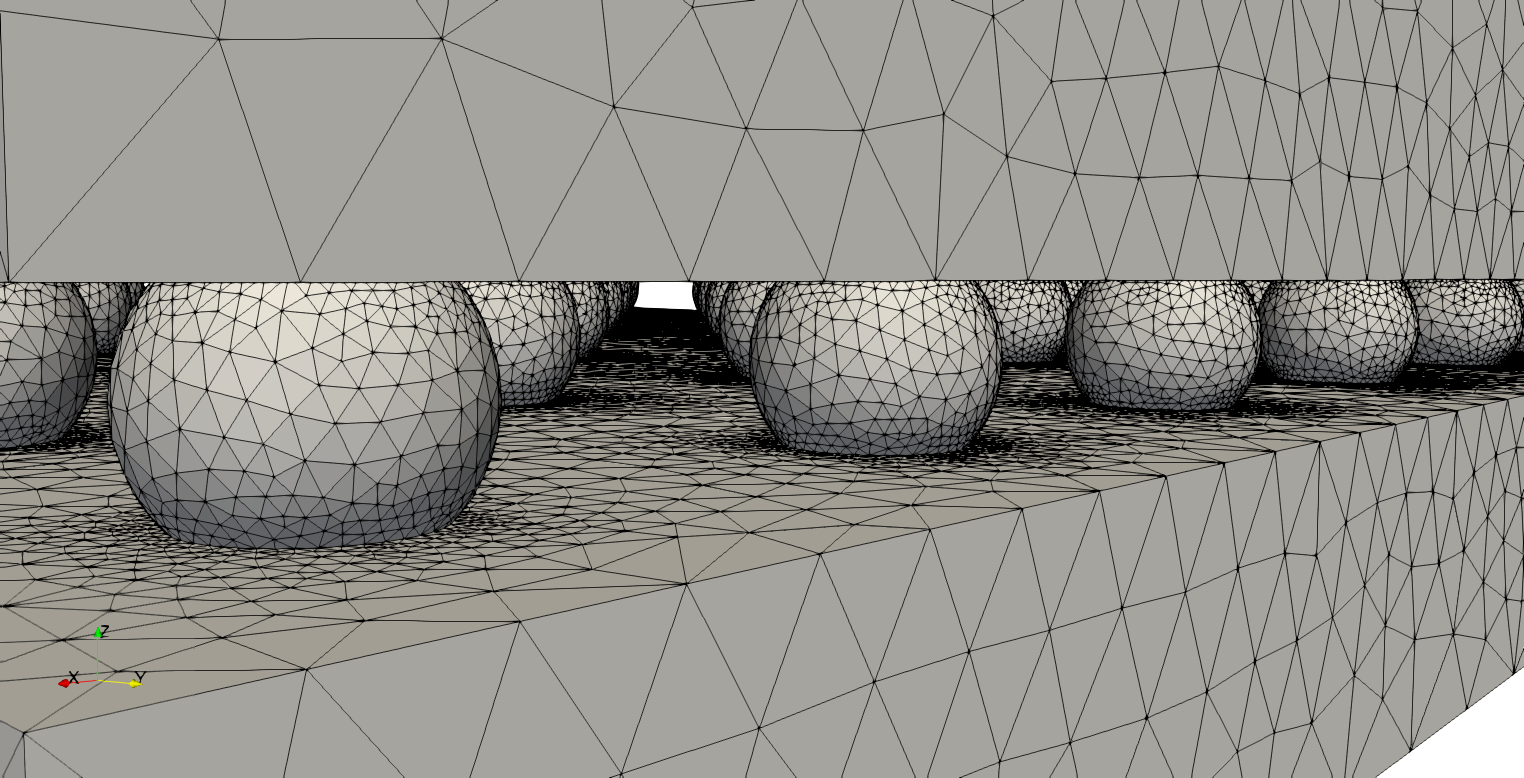
\includegraphics[width=.99\linewidth]{img/aut_solder_mesh_initial2.png}
\end{subfigure}%
\begin{subfigure}{0.5\textwidth}
\centering
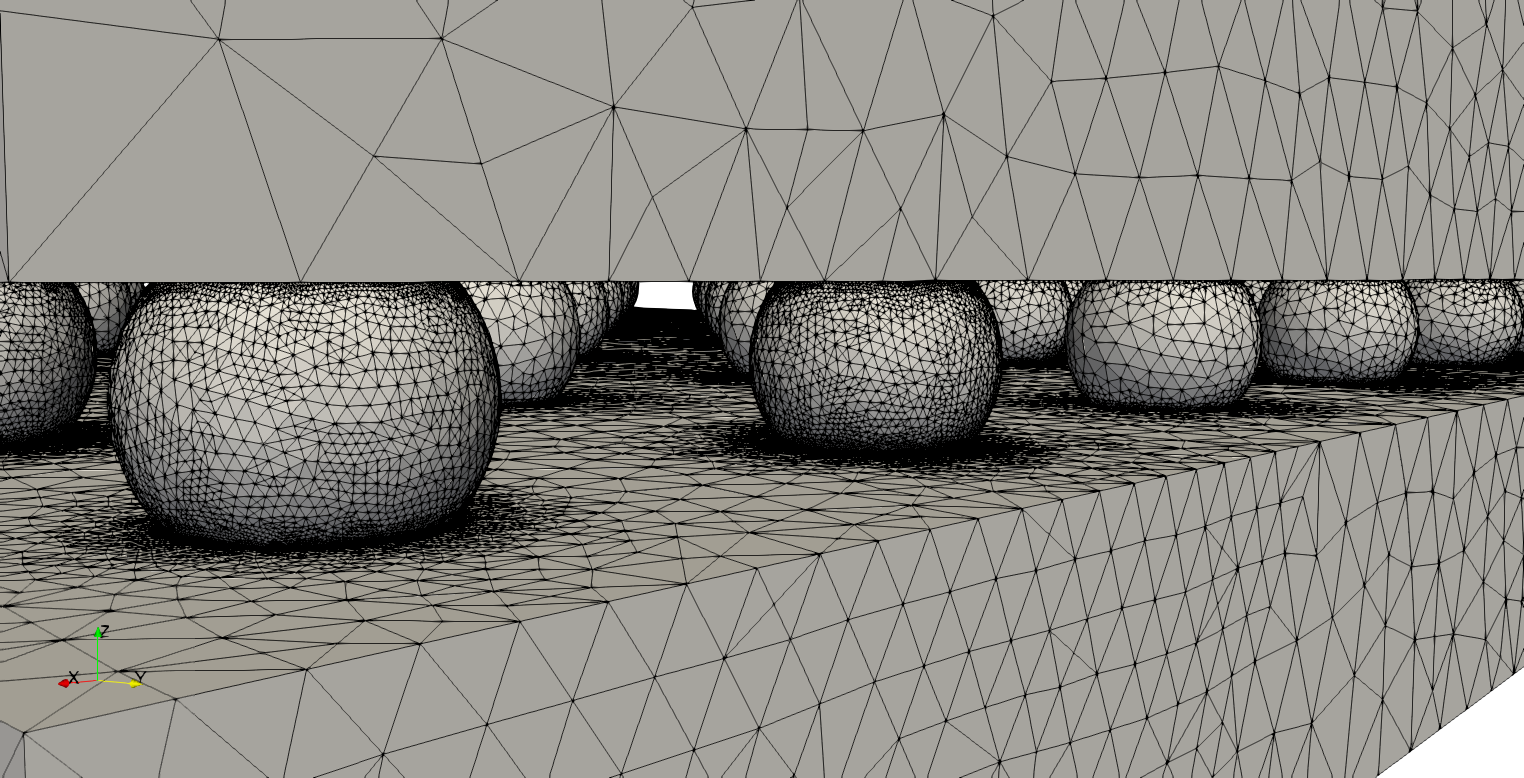
\includegraphics[width=.99\linewidth]{img/aut_solder_mesh_final2.png}
\end{subfigure}%
\caption{The initial mesh for the solder joint geometry (left) and the
final adapted mesh (right).}
\label{fig:aut_solder_mesh2}
\end{figure}

Figure \ref{fig:aut_solder_convergence} demonstrates the
convergence history of the error in the functional QoI,
as defined by the difference of the QoI obtained via
Richardson extrapolation and the QoI approximated by the
finite element solution. We compare the convergence for
two adaptive schemes, one achieved by successive uniform
refinements of the mesh and the other achieved by adjoint-based
error estimation. After 4 adaptive iterations, the adjoint-based
adaptive procedure achieves nearly the same degree of accuracy
as the uniform refinement procedure with two orders of
magnitude fewer degrees of freedom.

\begin{figure}[ht!]
\centering
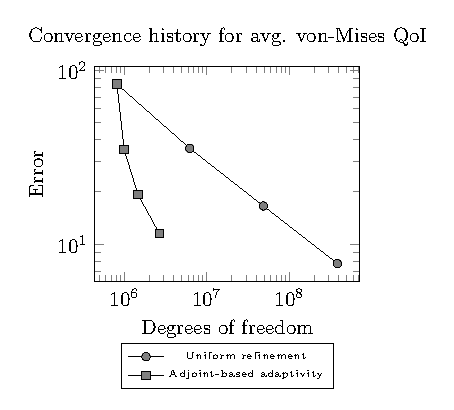
\includegraphics[width=0.5\linewidth]{img/aut_solder_convergence.pdf}
\caption{Error convergence histories for the solder joint example problem
with the average von-Mises stress QoI.}
\label{fig:aut_solder_convergence}
\end{figure}

Finally, we remark that automated parallel adaptive workflows
have been developed in reference \cite{bloomfield2017component}.
As an avenue for future investigation, adjoint-based error estimation
could be folded into these automated workflows.
In particular, an automated primal analysis could be used to inform
the actual selection of the QoI itself, which could then be accurately
assessed using adjoint-based error estimation.

%%% CONCLUSIONS
\section{Conclusions}

In this work, we have developed an automated approach for
adjoint-based error estimation and mesh adaptation for
execution on parallel machines. We have developed this approach
to be applicable to both Galerkin and stabilized finite
element methods. To realize this approach, we have extended
the concept of \emph{template-based generic programming} for
PDE models to include the automatic localization of error
contributions using a partition of unity-based
localization approach. We have demonstrated that this approach
is effective for a variety of example applications, including
nonlinear elasticity and elastoplasticity.

\chapter{ADJOINT-BASED ERROR ESTIMATION AND MESH ADAPTATION
FOR STABILIZED FINITE DEFORMATION ELASTICITY}
\label{chap:mech}

\let\thefootnote\relax\footnotetext{
This chapter has been submitted to:
B.~N. Granzow, A.~A. Oberai, M.~S. Shephard,
``Adjoint-based error estimation and mesh adaptation for
stabilized finite deformation elasticity,'' submitted for publication.}

%%% INTRODUCTION
\section{Introduction}

The purpose of this chapter is to develop an approach for functional error
estimation and mesh adaptation using adjoint-based techniques for
incompressible finite deformation elasticity. An important scenario where
incompressible nonlinear elastic materials are utilized is the study of
biological soft tissues \cite{legant2010measurement, paszek2005tensional,
discher2005tissue}. Adjoint-based error estimation provides the ability
to approximate discretization errors for a functional quantity of interest
(QoI) \cite{venditti2000adjoint, becker2001optimal, giles2002adjoint,
peraire1998bounds, prudhomme1999goal, braack2003posteriori,
bangerth2013adaptive}, such as point-wise displacements or stresses, or the
average displacement over a sub-domain. Mesh adaptation utilizes local
information obtained from error estimates to control discretization
errors by adaptively modifying the computational mesh.

Previously, in the context of solid mechanics, adaptive adjoint-based error
estimation has been used to study linear elasticity in two
\cite{rannacher1997feed, stein2007error, gonzalez2014mesh} and three
\cite{ghorashi2014goal} dimensional elasticity, two
\cite{rannacher1998posteriori, rannacher1999posteriori} and three
\cite{ghorashi2017goal} dimensional elasto-plasticity, two dimensional
thermoelasticity \cite{rabizadeh2015adaptive}, two dimensional nonlinear
elasticity \cite{larsson2002strategies}, and two dimensional
hyperelasticity \cite{whiteley2014error}. In the vast majority of the
previous literature, mesh adaptation is performed with structured adaptive
mesh refinement using quadrilateral or hexahedral elements. However, for
complex geometries such as those that arise in the study of biological
tissues, mesh generation and mesh adaptation are reliable, robust, and
scalable for simplical elements. This motivates us to consider triangular and
tetrahedral elements.

It is well known that solid mechanics problems with incompressibility
constraints perform poorly with linear displacement-based Galerkin finite
element methods when using simplical elements. This motivates us to consider
a mixed displacement-pressure based finite element formulation with an
additional pressure stabilization term. This is in contrast to the work by
Whiteley and Tavener \cite{whiteley2014error}, who utilized a Taylor-Hood
type element to study adjoint-based error estimation in two-dimensional
hyperelasticity.

In this work, we propose the following adaptive adjoint-based error
estimation strategy. First, we solve the primal finite deformation
elasticity problem with a stabilized mixed displacement-pressure finite
element method. Next, we construct and solve a discrete adjoint problem
in a finer space obtained via uniform mesh refinement. We then estimate
the global error in a functional QoI with a scaled discrete adjoint
weighted residual error estimate. To localize error estimates to the
mesh entity level, we utilize a recently developed approach
\cite{richter2015variational, wick2016goal} based on the insertion of
partition of unity (PU) into the variational form of the adjoint-weighted
residual error representation. Finally, utilizing these localized errors,
we perform fully unstructured mesh adaptation utilizing a series
of splits, swaps, and collapses.

The contributions of this work can be summarized as follows. First,
we expand upon the existing literature in solid mechanics to account for
stabilized finite element methods in adjoint-based error estimation.
Additionally, we propose a simple error correction to the well-known
adjoint-weighted residual \cite{fidkowski2011review} error estimate to obtain
more accurate error estimates when uniform refinement is used to compute the
adjoint solution. Next, we extend the PU-based error localization approach
of Richter and Wick \cite{richter2015variational} to the context of
stabilized finite element methods. Finally, we demonstrate that our adaptive
adjoint-based error estimation approach can be applied to realistic
three-dimensional engineering models, with greater geometric complexity
than we have seen in the existing literature.

The remainder of this chapter proceeds as follows. First, we review the
governing equations for a mixed displacement-pressure based formulation of
nonlinear finite deformation elasticity. Next, we review the development of
a mixed stabilized finite element method with equal order linear interpolants
for displacements and pressures over simplical elements. We then review the
so-called adjoint-weighted residual approach for functional error estimation
using two discretization levels, as defined by a coarse and a fine space.
After this review, We motivate our choice for the fine space, as achieved
by uniform mesh refinement. We then introduce a modified, more accurate
adjoint-weighted residual error estimate based on an \emph{a priori}
analysis. Next, we discuss the localization of the error estimate to the
mesh entity level by a recently developed PU approach, which we extend to
stabilized finite element methods. We then apply adaptive adjoint-based
analysis to a well known test case, the Cook's membrane problem to validate
and demonstrate the effectiveness of our approach. We then investigate and
demonstrate the utility of adjoint-based error estimation and mesh adaptation
for a three-dimensional example, motivated by the study of a cell embedded in
a matrix. Finally, we conclude by summarizing our results.

%%% MODEL PROBLEM
\section{Model Problem}

In this section, we introduce the governing equations for finite deformation
elasticity in a total Lagrangian setting with a neo-Hookean constitutive model.
We begin by presenting a mixed pressure-displacement formulation for the
strong form of the underlying PDE. We then present the corresponding weak form
of the PDE and review the derivation of a stabilized finite element
formulation. We conclude by discussing the linearization and solution
of the nonlinear system of equations resulting from the stabilized
finite element formulation.

%%% STRONG FORM
\subsection{Strong form}

Let $\B \subset \mathbb{R}^d$ denote the reference configuration of an open
bounded domain with smooth boundary $\Gamma$, where $d$ denotes the number of
spatial dimensions. Let $\Gamma$ be decomposed such that $\Gamma = \Gamma_g
\cup \Gamma_h$, where $\Gamma_g \cap \Gamma_h = \varnothing$. Let $\bs{X} \in
\B$ denote a point in the reference configuration which, after undergoing some
deformation, is located at the point $\bs{x} \in \B_t$ in the deformed
configuration at time $t$. Let $\bs{u} := \bs{x} - \bs{X}$ denote the
displacement vector. The deformation gradient is then defined as $\bs{F} :=
\bs{I} + \frac{\partial \bs{u}}{\partial \bs{X}}$, and we denote the
determinant of the deformation gradient as $J := \det(\bs{F})$.

The balance of linear momentum in the absence of inertial and body forces
leads to the following boundary value problem in the reference configuration:
%
%% mech_linear_momentum
\begin{gather}
\begin{cases}
\begin{aligned}
- \nabla \cdot \bs{P} &= \bs{0}, && \bs{X} \in \B, \\
\bs{u} &= \bs{g}, && \bs{X} \in \Gamma_g, \\
\bs{P} \cdot \bs{n} &= \bs{h}, && \bs{X} \in \Gamma_h.
\end{aligned}
\end{cases}
\label{eq:mech_linear_momentum}
\end{gather}
%
Here, $\bs{P} := J \bs{\sigma} \bs{F}^{-T}$ denotes the first Piola-Kirchhoff
stress tensor, $\bs{g}$ denotes an externally applied displacement, $\bs{h}$
denotes an externally applied traction, $\bs{n}$ denotes the unit outward
normal to the boundary $\Gamma_h$, and $\bs{\sigma}$ denotes the Cauchy
stress tensor.

We consider a neo-Hookean constitutive model, where the stress response
is characterized by the relationship:
%
%% mech_neohookean_model
\begin{gather}
\bs{\sigma} =
\underbrace{\mu J^{-\frac53} \text{dev}(\bs{F}\bs{F}^T)}_{\bs{\sigma}'} +
\underbrace{\frac{\kappa}{2 J}(J^2 - 1)}_{p} \bs{I}.
\label{eq:mech_neohookean_model}
\end{gather}
%
Here $\mu$ denotes the shear modulus, $\kappa$ denotes the bulk modulus,
$\bs{I}$ is the second order identity tensor, and $\text{dev}(\cdot) :=
(\cdot) - \frac13 \text{trace}(\cdot) \bs{I}$ denotes the deviatoric component
of a second order tensor. The stress is decomposed as $\bs{\sigma} =
\bs{\sigma}' + p \bs{I}$ into deviatoric and volumetric components,
$\bs{\sigma}'$ and $p \bs{I}$, respectively.

With this decomposition of the Cauchy stress tensor, the divergence of the
first Piola-Kirchhoff stress tensor can be expressed as
%
%% mech_div_first_pk
\begin{gather}
\begin{aligned}
\nabla \cdot \bs{P} &= \nabla \cdot ( J \bs{\sigma} \bs{F}^{-T} ) \\
&= \nabla \cdot ( J (\bs{\sigma}' + p \bs{I}) \bs{F}^{-T} ) \\
&= \nabla \cdot ( J \bs{\sigma}' \bs{F}^{-T} ) +
\nabla \cdot ( J p \bs{F}^{-T} ) \\
&= \nabla \cdot ( J \bs{\sigma}' \bs{F}^{-T} ) + J \bs{F}^{-T} \nabla p.
\end{aligned}
\label{eq:mech_div_first_pk}
\end{gather}
%
Here, we have used the Piola identity $\nabla \cdot (J \bs{F}^{-T}) = 0$
in the fourth equality. Using the decomposition \eqref{eq:mech_div_first_pk}
and introducing the pressure \eqref{eq:mech_neohookean_model} as an unknown
variable, the model problem \eqref{eq:mech_linear_momentum} can be written
in mixed form as:
%
%% mech_strong_form
\begin{gather}
\begin{cases}
\begin{aligned}
- \nabla \cdot (J \bs{\sigma}' \bs{F}^{-T}) - J \bs{F}^{-T} \nabla p &= 0,
&& \bs{X} \in \B, \\
\frac{p}{k} - \frac{1}{2 J}(J^2 - 1) &= 0,
&& \bs{X} \in \B, \\
\bs{u} &= \bs{g}, && \bs{X} \in \Gamma_g, \\
\bs{P} \cdot \bs{n} &= \bs{h}, && \bs{X} \in \Gamma_h.
\end{aligned}
\end{cases}
\label{eq:mech_strong_form}
\end{gather}

%%% WEAK FORM
\subsection{Weak Form}

Let $\V_u$, $\V_w$, and $\V_p$ denote the displacement trial space,
the displacement test space, and the pressure trial and test space,
respectively, defined as
%
%% mech_disp_space_continuous
\begin{gather}
\V_u := \{ \bs{u} : \bs{u} \in \H^1(\B)^d \; , \;
\bs{u} = \bs{g} \; \text{on} \; \Gamma_g \},
\label{eq:mech_disp_space_continuous}
\end{gather}
%
%% mech_weight_space_continuous
\begin{gather}
\V_w := \{ \bs{w} : \bs{w} \in \H^1(\B)^d \; , \;
\bs{w} = \bs{0} \; \text{on} \; \Gamma_g \},
\label{eq:mech_weight_space_continuous}
\end{gather}
%
%% mech_pressure_space_continuous
\begin{gather}
\V_p := \{ p : p \in L^2(\B) \; \}.
\label{eq:mech_pressure_space_continuous}
\end{gather}
%
Here, $\H^1$ denotes the Sobolev space of square-integrable functions
with square integrable first derivatives and $L^2$ denotes the space
of square-integrable functions. The weak form is obtained by multiplying
the pressure equation by an arbitrary weighting function $q \in \V_p$
and integrating over the domain $\B$, and by multiplying the momentum
equation by an arbitrary weighting function $\bs{w} \in \V_w$ and integrating
by parts over the domain $\B$. Letting $\S := \V_u \times \V_p$,
$\V := \V_w \times \V_p$, $\bs{U} := [\bs{u}, p]$, and $\bs{W} := [\bs{w}, q]$,
this process results in the weak form: find $\bs{U} \in \S$ such that
%
%% mech_weak_form
\begin{gather}
\R_g(\bs{W} ; \bs{U}) = 0 \quad \forall \, \bs{W} \in \V.
\label{eq:mech_weak_form}
\end{gather}
%
Here the Galerkin residual $\R_g : \V \times \S \to \mathbb{R}$ is
defined as
%
%% mech_galerkin_residual
\begin{gather}
\begin{split}
\R_g(\bs{W} ; \bs{U}) :=
&\int_{\B} (J \bs{\sigma}' \bs{F}^{-T}) : \nabla \bs{w} \; \text{d} V
+ \int_{\B} (J p \bs{F}^{-T}) : \nabla \bs{w} \; \text{d} V + \\
& \int_{\B} \left[ \frac{p}{\kappa} - \frac{1}{2 J}(J^2 - 1) \right] \;
q \; \text{d} V
- \int_{\Gamma_h} \bs{h} \cdot \bs{w} \; \text{d} A.
\end{split}
\label{eq:mech_galerkin_resid}
\end{gather}

%%% STABILIZED FINITE ELEMENT FORMULATION
\subsection{Stabilized Finite Element Formulation}

Consider a partitioning of the reference domain $\B$ into $n_{el}$
non-overlapping finite element sub-domains $\B_e$ such that $\B =
\cup_{e=1}^{n_{el}} \B_e$ and $\B_i \cap \B_j = \varnothing$ if $i \neq j$.
Let $\V^H_u \subset \V_u$, $\V^H_w \subset \V_w$, and $\V^H_p \subset \V_p$
denote finite dimensional function spaces defined as:
%
%% mech_disp_space
\begin{gather}
\V^H_u = \{ \bs{u}^H : \bs{u}^H \in \V_u \; , \;
\bs{u}^H |_{\bs{X} \in \B_e} \in \mathbb{P}^1 (\B_e)^d \},
\label{eq:mech_disp_space}
\end{gather}
%
%% mech_weight_space
\begin{gather}
\V^H_w = \{ \bs{w}^H : \bs{w}^H \in \V_w \; , \;
\bs{w}^H |_{\bs{X} \in \B_e} \in \mathbb{P}^1 (\B_e)^d \},
\label{eq:mech_weight_space}
\end{gather}
%
%% mech_press_space
\begin{gather}
\V^H_p = \{ p^H : p^H \in \V_p \; , \;
p^H |_{\bs{X} \in \B_e} \in \mathbb{P}^1 (\B_e) \}
\label{eq:mech_press_space}
\end{gather}
%
Here $\mathbb{P}^1(\B_e)$ denotes the space of piecewise linear polynomials
over elements $B_e$, $e=1,2,\dots,n_{el}$.

We follow the approach of Maniatty et al. \cite{klaas1999stabilized,
maniatty2002higher, ramesh2005stabilized} to obtain a stabilized
Petrov-Galerkin finite element formulation of the primal problem.
This approach proceeds by multiplying the momentum equation by a perturbed
weighting function of the form $\bs{w}^H + \tau_e \bs{F}^{-T} \nabla q^H$
and integrating over the reference domain $\B$, and by multiplying the
pressure equation by a weighting function $q^H$ and integrating over the
domain $\B$.

Here $\tau_e = \frac{c_0 H_e^2}{2 \mu}$ is a mesh-dependent stabilization
parameter, where $H_e = \text{meas}(\B_e)$ denotes a characteristic size
of a given mesh element, $\mu$ denotes the shear modulus, $c_0$ denotes a
non-dimensional, non-negative stability constant, $\bs{w}^H \in \V^H_w$ is
a displacement weighting function, and $q^H \in \V^H_p$ is a
pressure weighting function. Additionally, $\bs{F}^{-T} \nabla q^H$
represents the pull-back of the gradient of the pressure weighting function
to the reference configuration.

This yields the following problem: find $(\bs{u}^H, p^H) \in (\V^H_u, \V^H_p)$
such that for all $(\bs{w}^H, q^H) \in (\V^H_w, \V^H_p)$
%
%% mech_perturbed
\begin{gather}
\begin{split}
- \int_{\B} (\nabla \cdot \bs{P}) \cdot \bs{w}^H \; \text{d} V +
& \int_{\B} \left[ \frac{p^H}{\kappa} - \frac{1}{2 J}(J^2 - 1) \right] \;
q^H \; \text{d} V - \\
\sum_{e=1}^{n_{el}} & \int_{\B_e} (\nabla \cdot \bs{P}) \cdot
(\tau_e \bs{F}^{-T} \nabla q^H) \; \text{d} V = 0.
\label{eq:mech_perturbed}
\end{split}
\end{gather}
%
The first two terms on the left hand side of equation
\eqref{eq:mech_perturbed} yield the Galerkin residual
$\R_g(\bs{W}^H ; \bs{U}^H)$ after integrating the left-most term by parts.
The integrand of the third term on left hand side of equation
\eqref{eq:mech_perturbed} can be expressed as
%
%% mech_integrand_expand
\begin{gather}
\begin{split}
(\nabla \cdot \bs{P}) \cdot (\tau_e \bs{F}^{-T} \nabla q^H) \; = \;
&(\nabla \cdot J \bs{\sigma}' \bs{F}^{-T} ) \cdot
(\tau_e \bs{F}^{-T} \nabla q^H) + \\
&(\tau_e J \bs{F}^{-1} \bs{F}^{-T}) : (\nabla p^H \otimes \nabla q^H).
\label{eq:mech_integrand_expand}
\end{split}
\end{gather}
%
We remark that the first term in the right hand side of equation
\eqref{eq:mech_integrand_expand} evaluates to zero for simplical elements
with linear shape functions, which we presently consider.

Let $\S^H = \V^H_u \times \V^H_p$, $\V^H = \V^H_w \times \V^H_p$,
$\bs{U}^H = [ \bs{u}^H, p^H ]$, and $\bs{W}^H = [ \bs{w}^H, q^H ]$.
Using equations \eqref{eq:mech_galerkin_resid} and
\eqref{eq:mech_integrand_expand} in the perturbed weak problem
\eqref{eq:mech_perturbed}, we arrive at the stabilized finite element
formulation: find $\bs{U}^H \in \S^H$ such that
%
%% mech_stabilized_fem
\begin{gather}
\R_g(\bs{W}^H ; \bs{U}^H) + \R_{\tau}(\bs{W}^H ; \bs{U}^H) = 0
\quad \forall \, \bs{W}^H \in \V^H.
\label{eq:mech_stabilized_fem}
\end{gather}
%
Here $\R_{\tau} : \V^H \times \S^H \to \mathbb{R}$ is the residual
corresponding to the additional pressure stabilization, given by:
%
%% mech_stabilized_resid
\begin{gather}
\R_{\tau}(\bs{W}^H ; \bs{U}^H) :=
\sum_{e=1}^{n_{el}} \int_{\B_e} \tau_e
(J \bs{F}^{-1} \bs{F}^{-T}) : (\nabla p^H \otimes \nabla q^H) \; \text{d} V.
\end{gather}
%
We remark that we have introduced a consistent stabilization term, in that
$\R_{\tau} \to 0$ as $H \to 0$.

%%% LINEARIZATION AND SOLUTION STRATEGY
\subsection{Linearization and Solution Strategy}

The stabilized finite element formulation \eqref{eq:mech_stabilized_fem}
posed in residual form leads to a system of $N$ nonlinear algebraic equations
$\bs{R}^H : \mathbb{R}^N \to \mathbb{R}^N$, such that the numerical solution
vector $\bs{U}^H \in \mathbb{R}^N$ of nodal coefficients satisfies
%
%% mech_coarse_resid
\begin{gather}
\bs{R}^H(\bs{U}^H) = \bs{0}.
\label{eq:mech_coarse_resid}
\end{gather}
%
We compute consistent element-level tangent stiffness matrices via automatic
differentiation \cite{chen2014automatic} of element-level contributions to the
residual vector $\bs{R}^H$ to assemble the system Jacobian
$\bs{\J}^H \in \mathbb{R}^{N \times N}$, defined as
%
%% mech_jacobian
\begin{gather}
\bs{\J}^H(\bs{U}^H) :=
\frac{ \partial \bs{R}^H } { \partial \bs{U}^H } \biggr|_{\bs{U}^H}.
\label{eq:mech_jacobian}
\end{gather}
%
The full nonlinear problem \eqref{eq:mech_coarse_resid} is then solved with
Newton's method, where we iterate over the steps
%
%% mech_newtons
\begin{gather}
\begin{aligned}
\bs{\J}^H ( \bs{U}^H_k ) \, \delta \bs{U}^H_k &=
- \bs{R}^H( \bs{U}^H_k ) \\
\bs{U}^H_{k+1} &= \bs{U}^H_k + \delta \bs{U}^H_k,
\end{aligned}
\label{eq:mech_newtons}
\end{gather}
%
until the convergence criterion $\| \bs{R}^H(\bs{U}^H) \|_2 < \epsilon$
is satisfied for some user-specified tolerance $\epsilon$. Here
$\bs{U}^H_k$ denotes the solution vector at the $k^{th}$ Newton iteration
and $\delta \bs{U}^H_K$ denotes the incremental update at the $k^{th}$
iteration obtained by solving the Newton linear system.

%%% ADJOINT-BASED ERROR ESTIMATION
\section{Adjoint-Based Error Estimation}

In this section we derive an adjoint-based error estimation strategy to
compute errors in functional quantities of interest. We begin by reviewing
functional error estimation with two discretization levels, defined by a
\emph{coarse} space and a \emph{fine} space. Next, we discuss and motivate
our choice for the fine space. We then introduce a modified, more accurate
functional error estimate based on a simple \emph{a priori} analysis.
Finally, we conclude by discussing how we localize the functional error
to \emph{correction indicators} at the mesh entity level.

%%% ERROR ESTIMATION
\subsection{Two-Level Error Estimation}

Let $J(\bs{U})$ denote a functional quantity that is of physical significance.
We adopt a two-level error estimation strategy \cite{venditti2000adjoint,
venditti2002adjoint, venditti2003adjoint, fidkowski2011review} to estimate
the discretization error in $J$. This strategy proceeds by defining a
\emph{coarse} space, defined in the present setting by the spaces
$(\S^H, \V^H)$, and a \emph{fine} space, $(\S^h, \V^h)$.

In addition to the system of nonlinear algebraic equations
\eqref{eq:mech_coarse_resid} defined on the coarse space $(\S^H, \V^H)$,
the stabilized finite element formulation \eqref{eq:mech_stabilized_fem}
posed in residual form on the fine space $(\S^h, \V^h)$ leads to a system
of $n$ nonlinear algebraic equations $\bs{R}^n : \mathbb{R}^n \to
\mathbb{R}^n$ on the fine space, such that
%
%% mech_fine_resid
\begin{gather}
\bs{R}^h(\bs{U}^h) = \bs{0},
\label{eq:mech_fine_resid}
\end{gather}
%
where $\bs{U}^h \in \mathbb{R}^n$ is understood to be the solution vector
of nodal coefficients for the fine problem \eqref{eq:mech_fine_resid}.
Here $n > N$. Similarly, the functional quantity of interest can be
discretized on the coarse and fine spaces, resulting in $J^H : \mathbb{R}^N
\to \mathbb{R}$ and $J^h : \mathbb{R}^n \to \mathbb{R}$, respectively.

Let $\bs{U}^h_H = \bs{I}^h_H \bs{U}^H$ denote the prolongation of the coarse
solution $\bs{U}^H$ onto the fine space $\S^h$ via interpolation, where
$\bs{I}^h_H : \S^H \to \S^h$. The residual equations on the coarse space can
be expanded in a Taylor series about the prolongated coarse solution as
%
%% mech_residual_taylor
\begin{gather}
\bs{R}^h(\bs{U}^h) = \bs{R}^h(\bs{U}^h_H) +
\left[ 
\frac{ \partial \bs{R}^h }{ \partial \bs{U}^h} \biggr|_{\bs{U}^h_H}
\right]
(\bs{U}^h - \bs{U}^h_H) + \dots
\label{eq:mech_residual_taylor}
\end{gather}
%
and similarly, the functional evaluated on the coarse space can be expanded
about the prolongated coarse solution as
%
%% mech_functional_taylor
\begin{gather}
J^h(\bs{U}^h) = J^h(\bs{U}^h_H) +
\left[
\frac{ \partial J^h } { \partial \bs{U}^h} \biggr|_{\bs{U}^h_H}
\right]
(\bs{U}^h - \bs{U}^h_H) + \dots
\label{eq:mech_functional_taylor}
\end{gather}

Using equation \eqref{eq:mech_fine_resid}, the discretization error between
the two spaces can be approximated to first order as
%
%% mech_disc_error_approx
\begin{gather}
(\bs{U}^h - \bs{U}^h_H) \approx
- \left[
\frac{ \partial \bs{R}^h } { \partial \bs{U}^h } \biggr|_{\bs{U}^h_H}
\right]^{-1}
\bs{R}^h (\bs{U}^h_H ).
\label{eq:mech_disc_error_approx}
\end{gather}
This approximation can then be substituted into the functional Taylor
expansion \eqref{eq:mech_functional_taylor} to yield the so-called
adjoint weighted residual,
%
%% mech_functional_error_approx
\begin{gather}
J^h(\bs{U}^h) - J^h(\bs{U}^h_H) \approx
- 
\underbrace{
\left[
\frac{ \partial J^h } { \partial \bs{U}^h } \biggr|_{\bs{U}^h_H}
\right]
\left[
\frac{ \partial \bs{R}^h } { \partial \bs{U}^h } \biggr|_{\bs{U}^h_H}
\right]^{-1}
}_{\bs{Z}^h}
\bs{R}^h (\bs{U}^h_H),
\label{eq:mech_adjoint_weighted_residual}
\end{gather}
%
where $\bs{Z}^h \in \mathbb{R}^n$ denotes the solution to the
\emph{adjoint problem}:
%
%% mech_adjoint_problem
\begin{gather}
\left[
\frac{ \partial \bs{R}^h } { \partial \bs{U}^h} \biggr|_{\bs{U}^h_H}
\right]^T
\bs{Z}^h =
\left[
\frac{ \partial J^h } { \partial \bs{U}^h } \biggr|_{\bs{U}^h_H}
\right]^T.
\label{eq:mech_adjoint_problem}
\end{gather}

%%% CHOICE OF FINE SPACE
\subsection{Choice of Fine Space}

Several options exist for the choice of the fine space and the
approximation of the adjoint problem \eqref{eq:mech_adjoint_problem}.
The fine space can be defined by uniformly refining the mesh, which
we will refer to as $h$-enrichment, increasing the polynomial interpolation
order, which we will refer to as $p$-enrichment, uniformly refining
the mesh and increasing the polynomial order, which we will refer to as
$hp$-enrichment, or by considering a finer space provided by variational
multiscale techniques \cite{granzow2017output}.

It is common to solve the adjoint problem
\eqref{eq:mech_adjoint_problem} in the coarse space and then perform
a reconstruction process to recover an approximation of the adjoint
solution on the fine space \cite{nemec2007adjoint, lu2005posteriori,
fidkowski2006output, becker2001optimal}. However, the most commonly used
choices for reconstruction do not incorporate the underlying physics of the
problem, and thus are not guaranteed to result in a more accurate
approximation of the adjoint solution \cite{fidkowski2011review}.
This motivates us to solve the adjoint problem globally on the fine space
\cite{barth2002aposteriori, hartmann2002adaptive}.

In the present work, we choose $h$-enrichment for the fine space.
Along with the previously discussed accuracy considerations, we are motivated
to do so for two additional reasons. First, the use of a higher order basis
ala $p$-enrichment would necessitate the inclusion of the neglected higher
order stabilization term in the expansion \eqref{eq:mech_integrand_expand}.
This term is generally non-trivial to implement \cite{maniatty2002higher}.
Second, we remark that higher-order stabilized finite element methods with
equal order interpolants are rarely used in practice, as one could use a
Taylor-Hood type element \cite{taylor1973numerical} to satisfy the
Babu\v{s}ka-Brezzi condition with much fewer degrees of freedom than the
corresponding stabilized finite element method with equal order interpolants.

%%% AN A-PRIORI ANALYSIS
\subsection{Modified Functional Error Estimate}

Consider that the functional of interest converges at the rate $k$, such
that $J(\bs{U}) - J^h(\bs{U}^h_H) = cH^k$ and $J(\bs{U}) - J^h(\bs{U}^h) =
ch^k$, where $J(\bs{U})$ is the exact value of the functional quantity of
interest. We assume that the fine space is obtained via mesh refinement,
such that $\frac{h}{H} = \frac12$. Consider the ratio
%
%% mech_ratio
\begin{gather}
\begin{aligned}
\frac{ J^h (\bs{U}^h) - J^h(\bs{U}^h_H) }{ J(\bs{U}) - J^h(\bs{U}^h_H) }
&= \frac{\left[ J^h(\bs{U}) - J^h(\bs{U}^h_H) \right] -
\left[ J^h(\bs{U}) - J^h(\bs{U}^h) \right] }
{ J(\bs{U}) - J^h(\bs{U}^h_H) } \\
&= \frac{c H^k - ch^k}{c H^k} \\
&= 1 - \left( \frac{h}{H} \right)^k \\
&= 1 - \left( \frac12 \right)^k
\end{aligned}
\end{gather}
%
in the limit as $H \to 0$ \cite{fidkowski2011review}. We denote this ratio
as $\alpha := 1 - (1/2)^k$. Let $\eta$ denote an approximation to the
functional error $J(\bs{U}) - J^h(\bs{U}^h_H)$. Let $\I$ denote the
effectivity index given by
%
%% mech_effectivity
\begin{gather}
\I = \frac{\eta}{ J(\bs{U}) - J^h(\bs{U}^h_H) }.
\label{eq:mech_effectivity}
\end{gather}
%
Naturally, we would like to obtain error estimates $\eta$ that lead to
effectivity indices of $\I = 1$ as $H \to 0$. To this end, we recall that
$J^h(\bs{U}^h) - J^h(\bs{U}^h_H) \approx - \bs{Z}^h \cdot
\bs{R}^h(\bs{U}^h_H)$ from equation \eqref{eq:mech_adjoint_weighted_residual}
and obtain the scaled adjoint weighted residual error estimate
%
%% mech_error_estimate
\begin{gather}
\eta = - \frac{1}{\alpha} \bs{Z}^h \cdot \bs{R}^h(\bs{U}^h_H).
\label{eq:mech_error_estimate}
\end{gather}

%%% ERROR LOCALIZATION
\subsection{Error Localization}

To drive mesh adaptation, it is necessary to localize contributions to the
total error $\eta$ to the mesh entity level to obtain
\emph{correction indicators}. One commonly used approached for finite volume
and discontinuous Galerkin methods proceeds by considering a decomposition
of the error estimate $\eqref{eq:mech_error_estimate}$ into a sum of discrete
adjoint weighted residuals over elements in the fine mesh. However, this
approach is not optimal for continuous finite elements as it does not account
for systematic inter-element cancellation, and the sum of the resulting
correction indicators would lead to a considerable over-estimation of
the functional error \cite{fidkowski2011review}. This, in turn, would lead to
a sub-optimal adaptive strategy.

Traditional adjoint-weighted residual error estimates for continuous Galerkin
finite element methods proceed by integrating the left hand side of equation
\eqref{eq:mech_stabilized_fem} by parts over individual elements to recover
strong-form volumetric and jump term contributions to the error. In this
work, we utilize a recently introduced localization strategy by Richter and
Wick \cite{richter2015variational} for its straightforward implementation
and because it allows us to automate the adaptive process. In this
localization,
adjoint-weighted residual error information from
neighboring elements is gathered by introducing a partition of unity,
leading to nodally-based correction indicators. In the context of solid
mechanics, this approach has been used successfully for phase field fracture
\cite{wick2016goal}. In this section, we extend this variational localization
technique to stabilized finite element methods.

We begin by reviewing adjoint-based error estimation for stabilized finite
element methods in a continuous setting, as outlined by Cyr et al.
\cite{cyr2014approaches}, for which we introduce the continuous linearized
adjoint problem: find $\bs{Z} \in \V$ such that
%
%% mech_continuous_adjoint
\begin{gather}
\R'_g[\bs{U}^H](\bs{V}, \bs{Z}) = J'[\bs{U}^H](\bs{V})
\quad \forall \; \bs{V} \in \V.
\label{eq:mech_continuous_adjoint}
\end{gather}
%
Here, the prime indicates Fr\'{e}chet linearization with respect to the
argument in the square brackets. The adjoint solution $\bs{Z} :=
[\bs{z}_u, z_p]$ is defined as a vector of the adjoint variable $\bs{z}_u$
corresponding to the primal displacement $\bs{u}$ and the adjoint variable
$z_p$ corresponding to the primal pressure $p$. The variable $\bs{U}^H$
denotes the solution to the stabilized finite element problem
\eqref{eq:mech_stabilized_fem} on the coarse space.

Let $\bs{E} := \bs{U} - \bs{U}^H$ denote the discretization error.
With the introduction of the adjoint problem
\eqref{eq:mech_continuous_adjoint}, a functional error representation can be
derived in the following manner:
%
%% mech_error_representation
\begin{gather}
\begin{aligned}
J(\bs{U}) - J(\bs{U}^H) &= J'[\bs{U}^H](\bs{E}) + \O(\bs{E}^2) \\
&= \R'_g[\bs{U}^H](\bs{E}, \bs{Z}) + \O(\bs{E}^2) \\
&= \R_g(\bs{Z}; \bs{U}) - \R_g(\bs{Z} ; \bs{U}^H) + \O(\bs{E}^2) \\
&= - \R_g(\bs{Z}; \bs{U}^H) + \O(\bs{E}^2) \\
&= - \R_g(\bs{Z} - \bs{Z}^H; \bs{U}^H) + \R_{\tau}(\bs{Z}^H; \bs{U}^H) +
\O(\bs{E}^2).
\end{aligned}
\label{eq:mech_error_representation}
\end{gather}
%
Here the first equality is due to the linearization \cite{becker2001optimal}
of the functional $J$, the second equality is due to the definition
of the adjoint problem \eqref{eq:mech_continuous_adjoint}, the third
equality is due to the linearization \cite{becker2001optimal} of the Galerkin
residual semilinear form $R_g$, the fourth equality is due to Galerkin
orthogonality, and the fifth equality holds by the definition of the
stabilized finite element method \eqref{eq:mech_stabilized_fem}.
The variable $\bs{Z}^H$ denotes the interpolant of the adjoint solution
$\bs{Z}$ onto the coarse finite element space $\S^H$.

Let $\bs{Z}^h$ denote the solution to the discrete adjoint problem
\eqref{eq:mech_adjoint_problem} solved on the fine space. We assume that
this solution well approximates the continuous adjoint problem
\eqref{eq:mech_continuous_adjoint}, such that $\bs{Z} \approx \bs{Z}^h$.
The functional error is then approximated by neglecting higher order terms
to obtain
%
%% mech_error_approx
\begin{gather}
J(\bs{U}) - J(\bs{U}^H) \approx
- \R_g(\bs{Z}^h - \bs{Z}^H; \bs{U}^H) + \R_{\tau}(\bs{Z}^H, \bs{U}^H).
\label{eq:mech_error_approx}
\end{gather}

Following the approach of Richter and Wick \cite{richter2015variational}, we
introduce a partition of unity $\sum_i \phi_i = 1$ into the weighting
function slot for the error estimate to localize the error. In this work,
this partition of unity is realized with linear Lagrange basis functions.
This yields local level error contributions $\eta_i$ at the $n_{vtx}$
mesh vertices in the fine mesh, given as
%
%% mech_error_localization
\begin{gather}
J(\bs{U}) - J(\bs{U}^H) \approx
\sum_{i=1}^{n_{vtx}}
\underbrace{
- \R_g ( (\bs{Z}^h - \bs{Z}^H) \phi_i \; ; \; \bs{U}^H ) +
\R_{\tau} ( \bs{Z}^H \phi_i \; ; \; \bs{U}^H )
}_{\eta_i}
\label{eq:mech_error_localization}
\end{gather}
%
We compute an approximate upper bound on the error by summing the absolute
value of the error contributions over all mesh vertices.
%
%% mech_approximated_bound
\begin{gather}
\hat{\eta} = \sum_{i=1}^{n_{vtx}} | \eta_i |
\label{eq:mech_approximated_bound}
\end{gather}
%
To compute an element-based correction indicator $\eta_e$, we interpolate the
value of the vertex-based error contributions $\eta_i$ to element centers
and then take the result's absolute value.

%%% MESH ADAPTATION
\section{Mesh Adaptation}

To control discretization errors, we make use of conforming unstructured
mesh adaptation. Mesh adaptation provides the means to modify the spatial
discretization of the domain $\B$ such that the degrees of freedom are nearly
optimally distributed with respect to the calculation of the QoI.
We utilize the PUMI \cite{ibanez2016pumi} software suite to perform a series
of edge splits, swaps, and collapses \cite{li20053d, alauzet2006parallel} to
satisfy the input of a \emph{mesh size field}. For isotropic mesh adaptation,
which we presently consider, the mesh size field is defined as a scalar field
that defines element edge lengths over the mesh. From a high-level, we would
like to specify a mesh size field that refines in areas of the domain that
strongly contribute to the error and coarsens the mesh in areas that are
insensitive to the error.

To this end, we utilize a size field specification following Boussetta et al.
\cite{boussetta2006adaptive} that attempts to equidistribute the error in an
output adapted mesh with $N$ target elements. Let $p$ be the polynomial
interpolant order for the chosen finite element method. In the present
setting, $p=1$. We first define the global quantity $G$ as
%
%% mech_global_size_quantity
\begin{gather}
G = \sum_{e=1}^{n_{el}} ( \eta_e ) ^{\frac{2d}{2p+d}}.
\label{eq:mech_global_size_quantity}
\end{gather}
%
Using this computed quantity, new element mesh sizes $H_e^{\text{new}}$ are
determined by scaling the previous element size $H_e$ according to the
formula
%
%% mech_size_field
\begin{gather}
H_e^{\text{new}} = \left( \frac{G}{N} \right)^{\frac{1}{d}}
( \eta_e )^{\frac{-2}{2p + d}} H_e
\label{eq:mech_size_field}
\end{gather}
%
Additionally, to prevent excessive refinement or coarsening in a single
adaptive step, we clamp the element size such that it is no smaller than
one quarter and no greater than twice the previous element size,
%
%% mech_size_clamping
\begin{gather}
\frac14 \leq \frac{H_e^{\text{new}}}{H_e} \leq 2.
\label{eq:mech_size_clamping}
\end{gather}
%
As a further explanation, this clamping is performed to ensure that mesh
adaptation is being driven by accurate correction indicators. That is,
if the mesh were too heavily modified during a single adaptive iteration,
the localized correction indicators would begin to lose accuracy on the
modified mesh.

%%% RESULTS
\section{Results}

%%% COOKS MEMBRANE
\subsection{Cook's Membrane}

In this section, we investigate two displacement-based quantities of
interest for Cook's membrane. The first QoI we consider is
the $y$-component of displacement at the point $\bs{X}_0 = (44,55)$ such
that $J_1(\bs{U}) = \int_{\B} \delta(\bs{X} - \bs{X}_0) \; u_y \, \text{d} V$. 
The second QoI we consider is the average displacement
over the entire domain, such that $J_2(\bs{U}) = \int_{\B} \frac12 (u_x + u_y)
\, \text{d} V$. Figure \ref{fig:cooks_geom} shows the geometry and loading
conditions for the Cook's membrane problem, where the left-most boundary
is fixed in the $x$ and $y$ directions and a purely vertical traction of
magnitude $10$ is applied to the right-most boundary. For material
properties, we choose the elastic modulus to be $E=1000$ and Poisson's
ratio as $\nu = 0.4999$, such that the material is in the incompressible
limit. We choose the stabilization parameter to be $c_0 = 1$. For both
quantities of interest, we expect the convergence rate to be $k = 2$, such
that the scaling parameter $\alpha = \frac34$.

\begin{figure}[ht!]
\centering
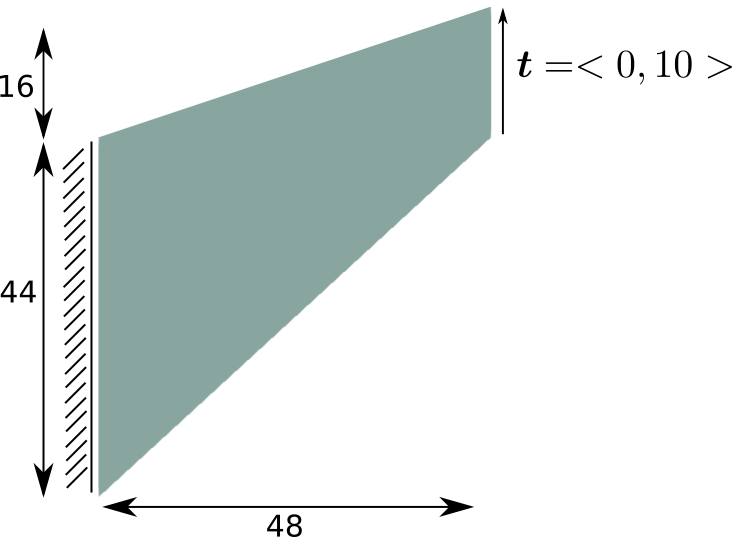
\includegraphics[width=0.4\textwidth]{img/mech_cooks_geom.png}
\caption{Cook's membrane problem definition.}
\label{fig:cooks_geom}
\end{figure}

For each QoI, an initial mesh with a uniform size of $H=8$
was generated. Figures \ref{fig:mech_cooks_pw_meshes} and
\ref{fig:mech_cooks_avg_u_meshes} show the initial mesh utilized for both
the point-wise and average displacement QoIs. From these initial meshes,
the steps
%
\begin{gather*}
\text{Solve primal PDE} \rightarrow
\text{Solve adjoint PDE} \rightarrow
\text{Localize error} \rightarrow
\text{Adapt mesh}
\end{gather*}
%
were iteratively performed until a final mesh with about $10,000$ degrees
of freedom was produced. During each mesh adaptation, the size field was
specified according to the equation \eqref{eq:mech_size_field} such that
the desired number of elements $N$ in the output mesh is twice the number
of elements in the previous mesh.

\begin{figure}[ht!]
\centering
\begin{subfigure}{.33\textwidth}
\centering
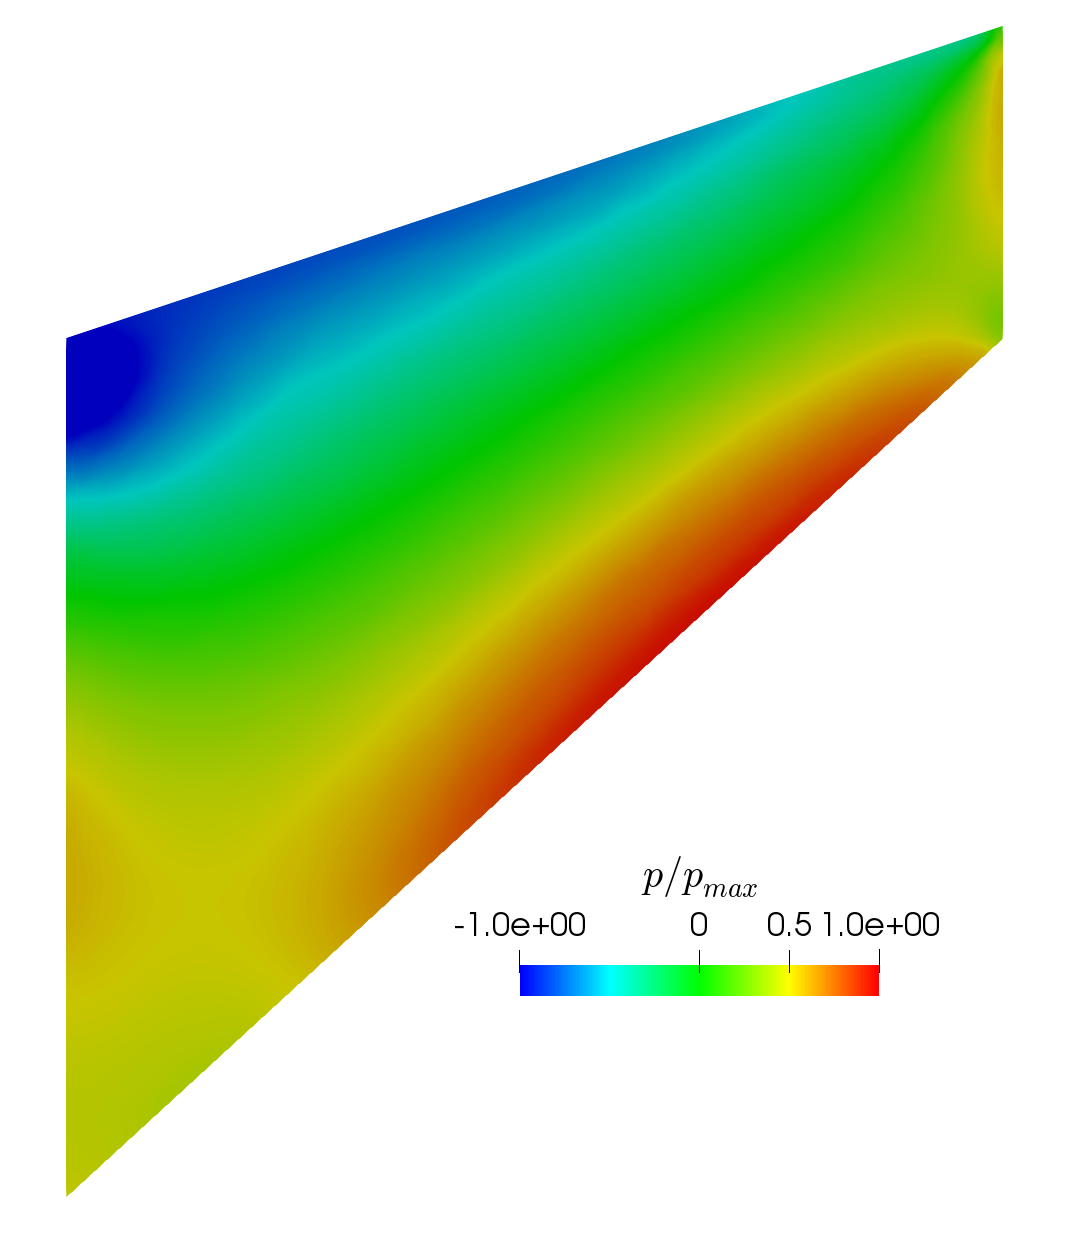
\includegraphics[width=.9\linewidth]{img/mech_cooks_pw_p.png}
\end{subfigure}%
\begin{subfigure}{.33\textwidth}
\centering
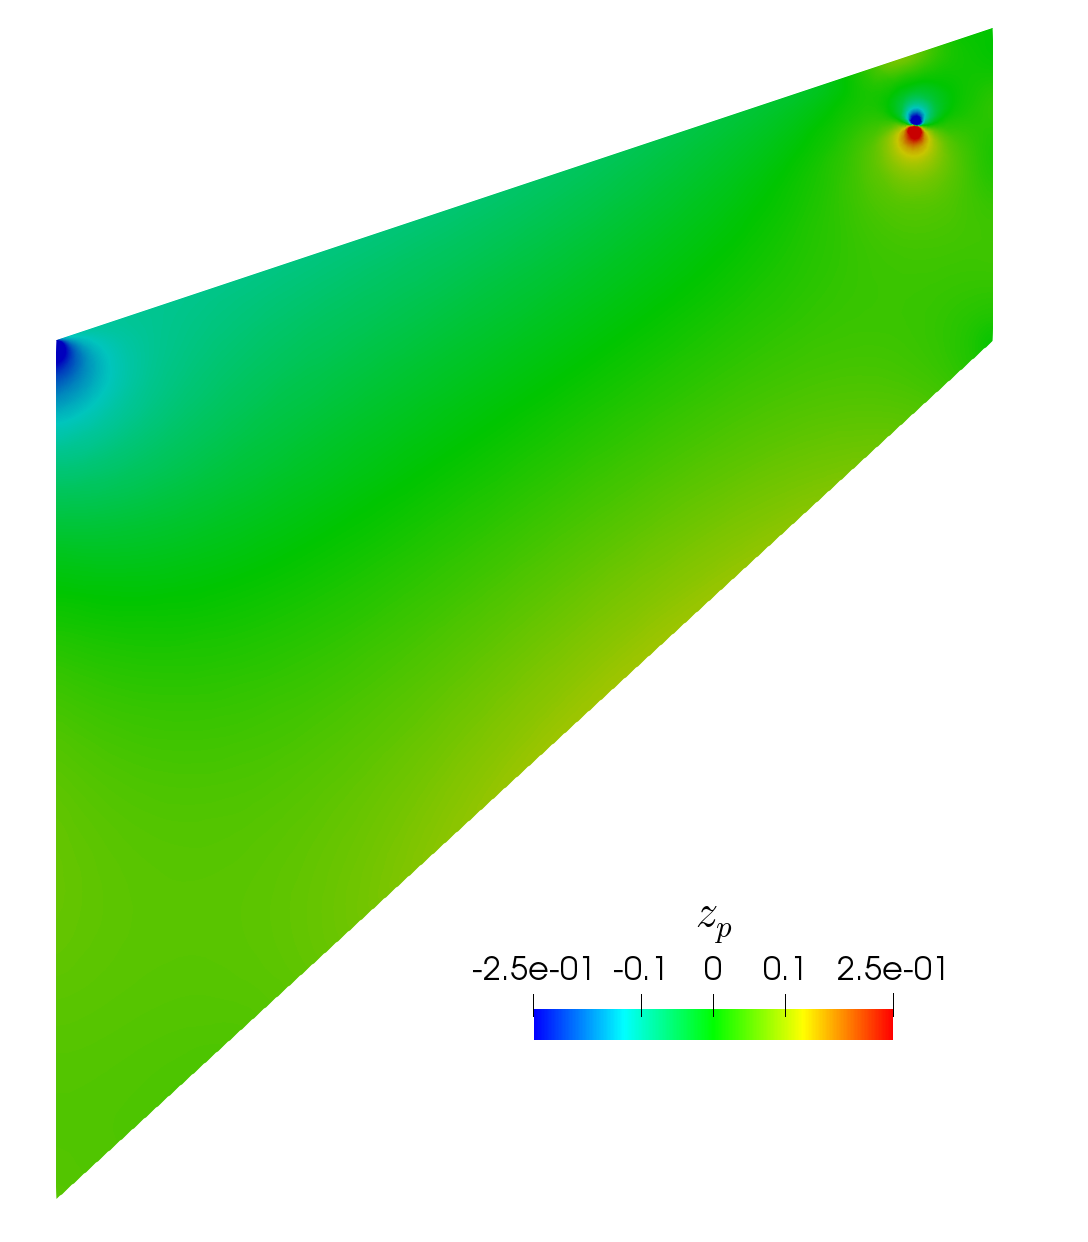
\includegraphics[width=.9\linewidth]{img/mech_cooks_pw_zp.png}
\end{subfigure}
\begin{subfigure}{.33\textwidth}
\centering
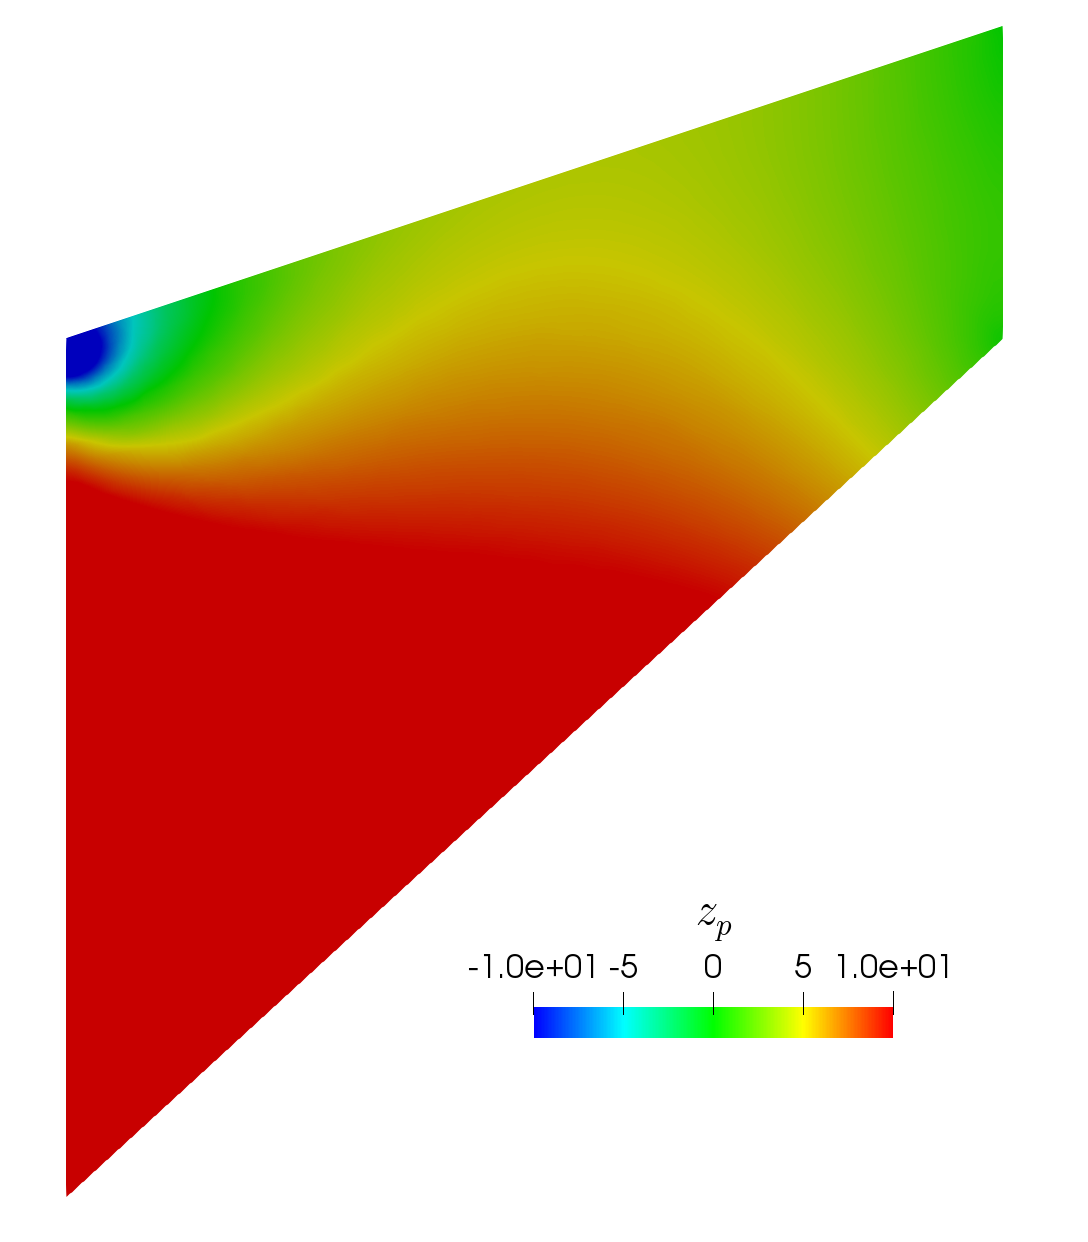
\includegraphics[width=.9\linewidth]{img/mech_cooks_avg_u_zp.png}
\end{subfigure}
\caption{The pressure component $p$ of the primal solution scaled by its
maximal value (left), the pressure component $z_p$ of the adjoint solution for
the point-wise QoI $J_1(\bs{U})$, and the pressure component $z_p$ of the
adjoint solution for the average displacement QoI $J_2(\bs{U})$.}
\label{fig:mech_cooks_pressures}
\end{figure}

The left-most figure of Figure \ref{fig:mech_cooks_pressures} illustrates
the pressure component $p$ of the primal solution scaled by its maximal
value. We remark that this result is consistent with previous literature
\cite{ostien2016tet}. The center and right-most figures of Figure
\ref{fig:mech_cooks_pressures} shows the pressure component $z_p$ of the
adjoint solution for the point-wise QoI $J_1(\bs{U})$ and the average
displacement QoI $J_2(\bs{U})$, respectively. For the point-wise QoI, the
adjoint solution $z_p$ is highly localized to the point that defines the
QoI and the corner of stress singularity.

\begin{figure}[ht!]
\centering
\begin{subfigure}{.5\textwidth}
\centering
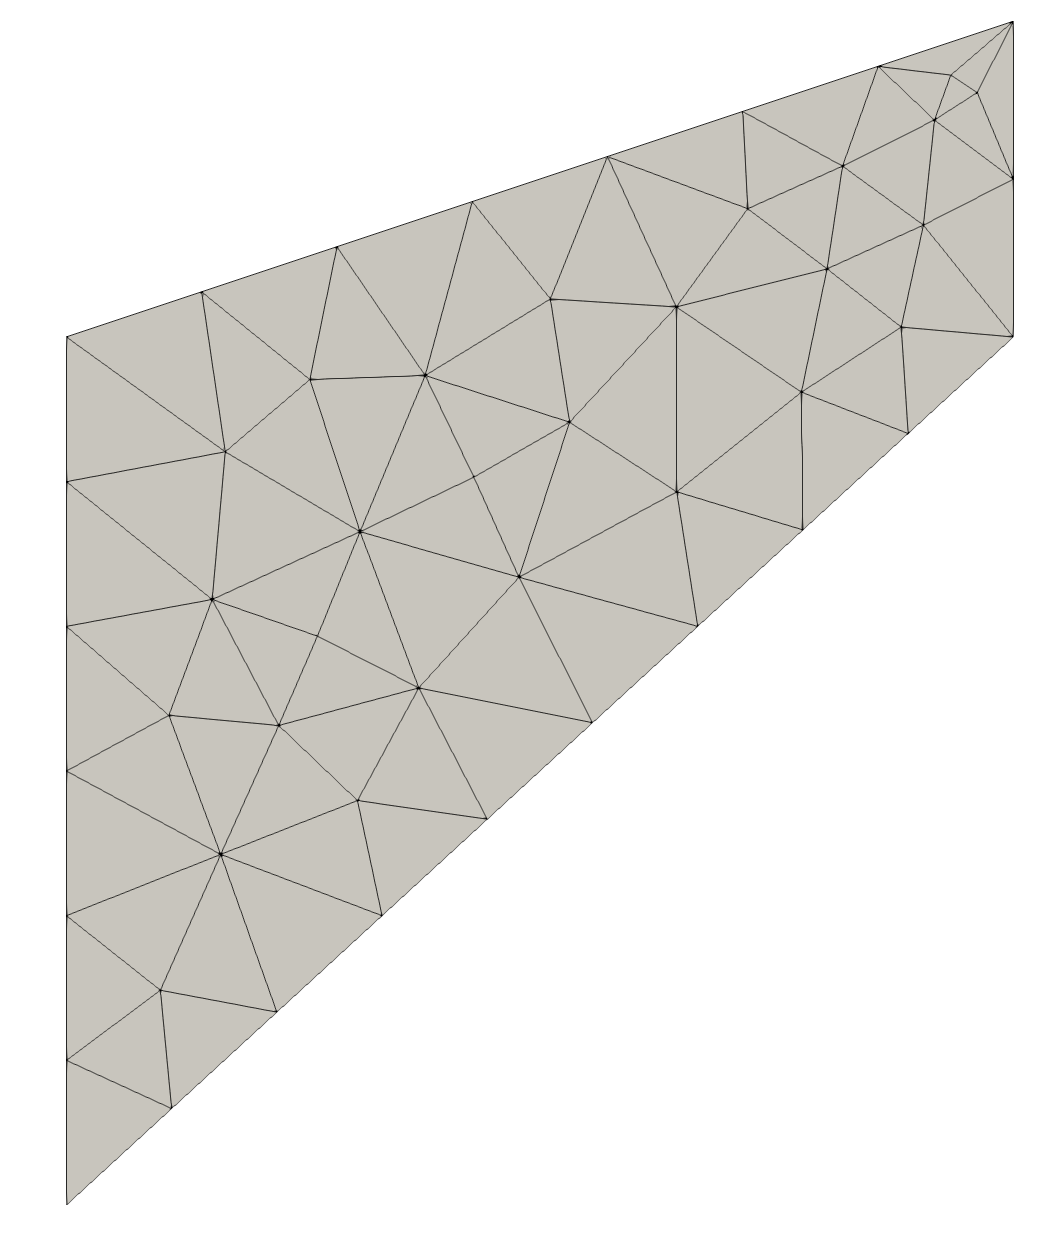
\includegraphics[width=.6\linewidth]{img/mech_cooks_pw_initial_mesh.png}
\end{subfigure}%
\begin{subfigure}{.5\textwidth}
\centering
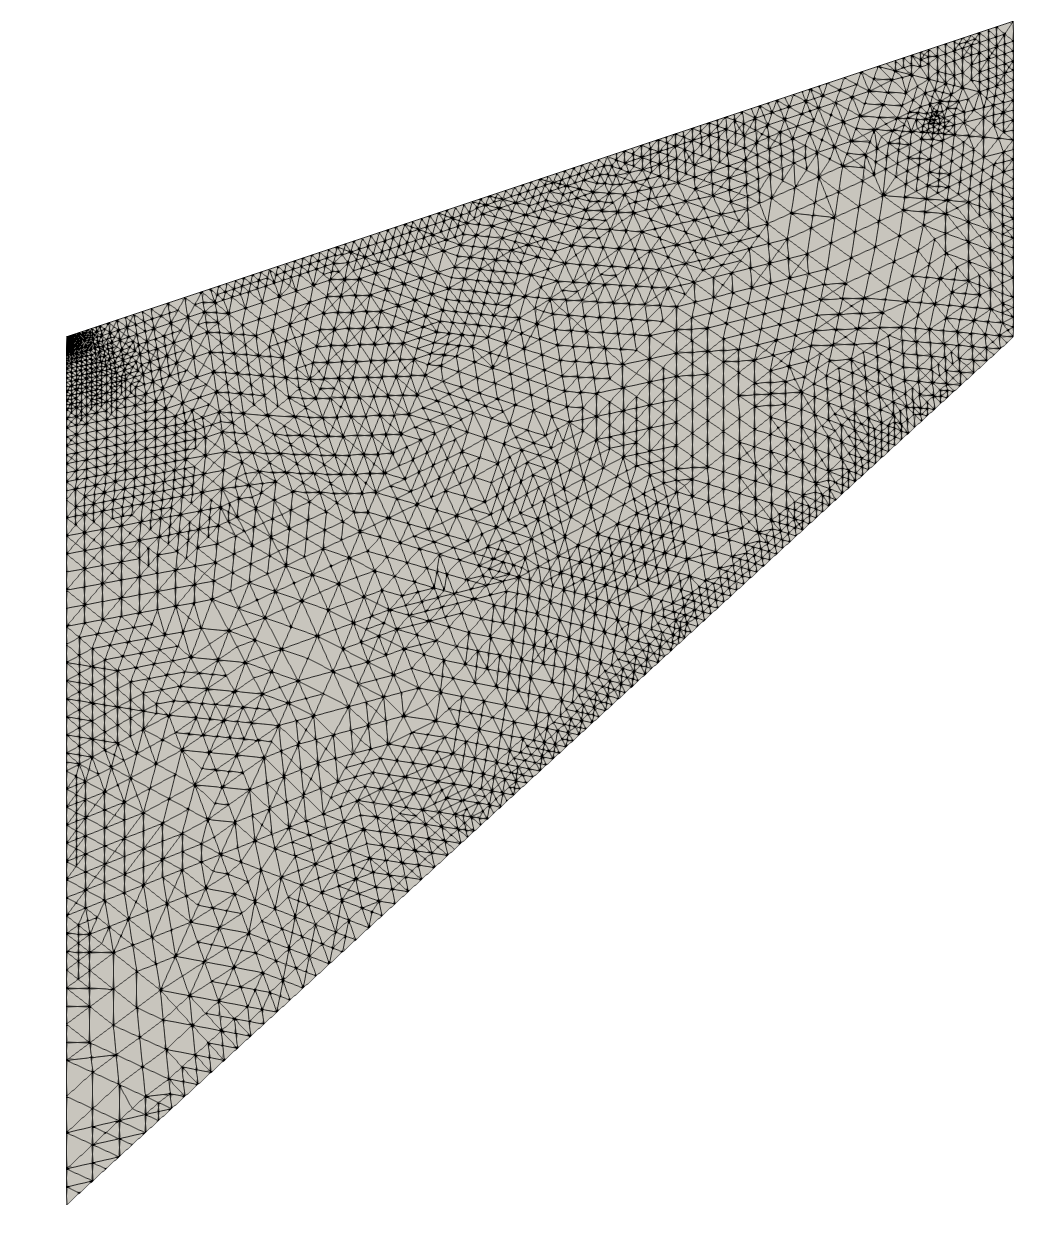
\includegraphics[width=.6\linewidth]{img/mech_cooks_pw_final_mesh.png}
\end{subfigure}
\caption{Initial mesh (left) and adapted mesh (right) at the fifth
adaptive iteration for the Cook's membrane problem with the point-wise
QoI $J_1(\bs{U})$.}
\label{fig:mech_cooks_pw_meshes}
\end{figure}

To approximate the exact values of the quantities of interest, the primal
problem was solved on a ``truth'' mesh with about $1.5$ million degrees of
freedom. This mesh is finer at every spatial location than the final meshes
produced by the two adaptive simulations. The reference value for the
point-wise QoI on the truth mesh was computed to be
$J_1(\bs{U}) = 2.395627$ and the reference value for the average displacement
QoI was computed to be $J_2(\bs{U}) = 324.0948$.

\begin{figure}[ht!]
\centering
\begin{subfigure}{.5\textwidth}
\centering
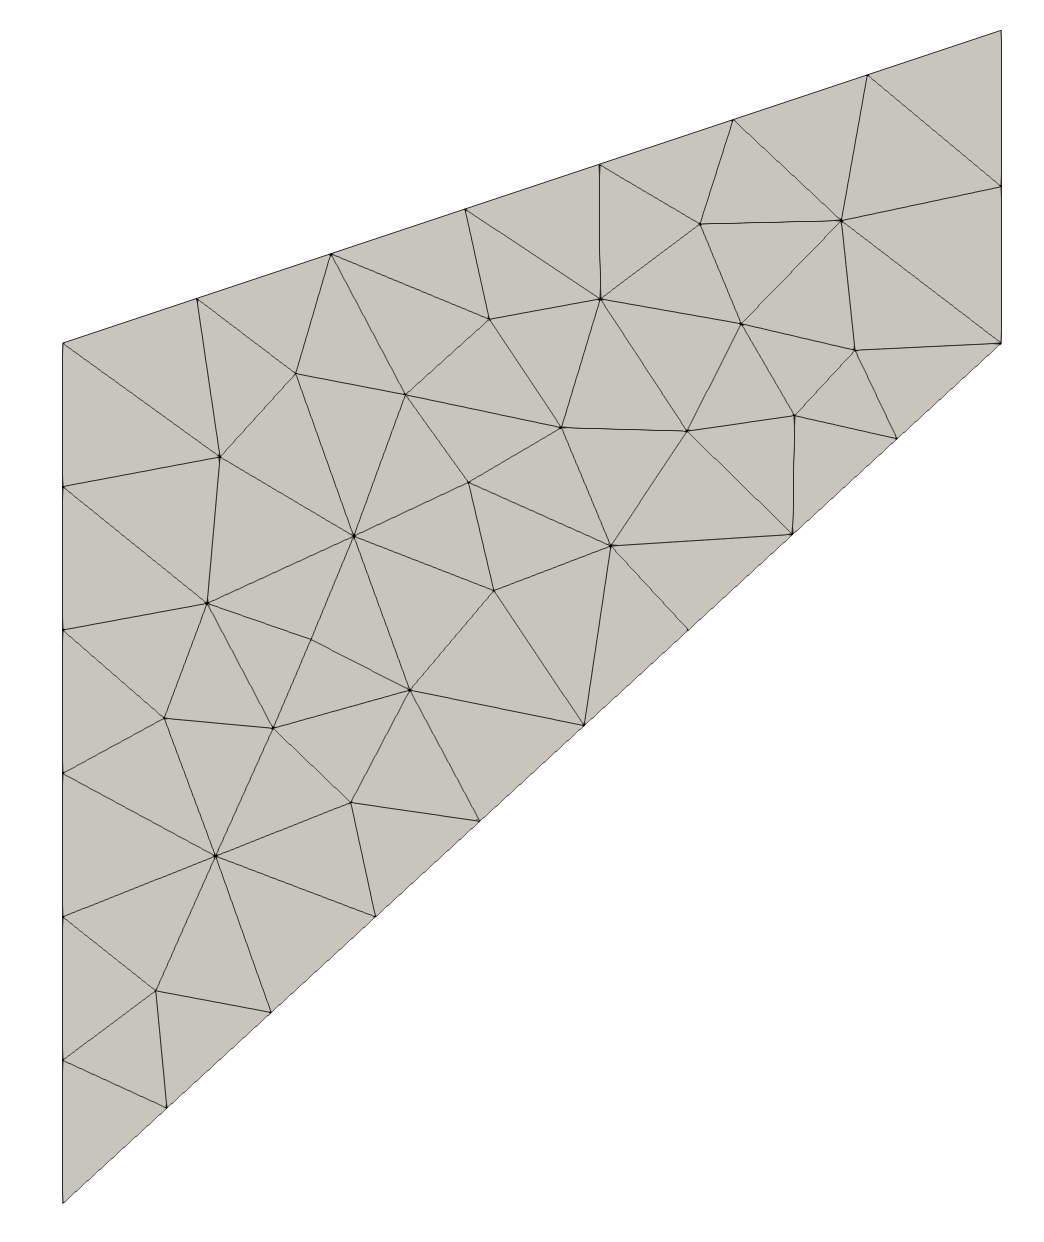
\includegraphics[width=.6\linewidth]{img/mech_cooks_avg_u_initial_mesh.png}
\end{subfigure}%
\begin{subfigure}{.5\textwidth}
\centering
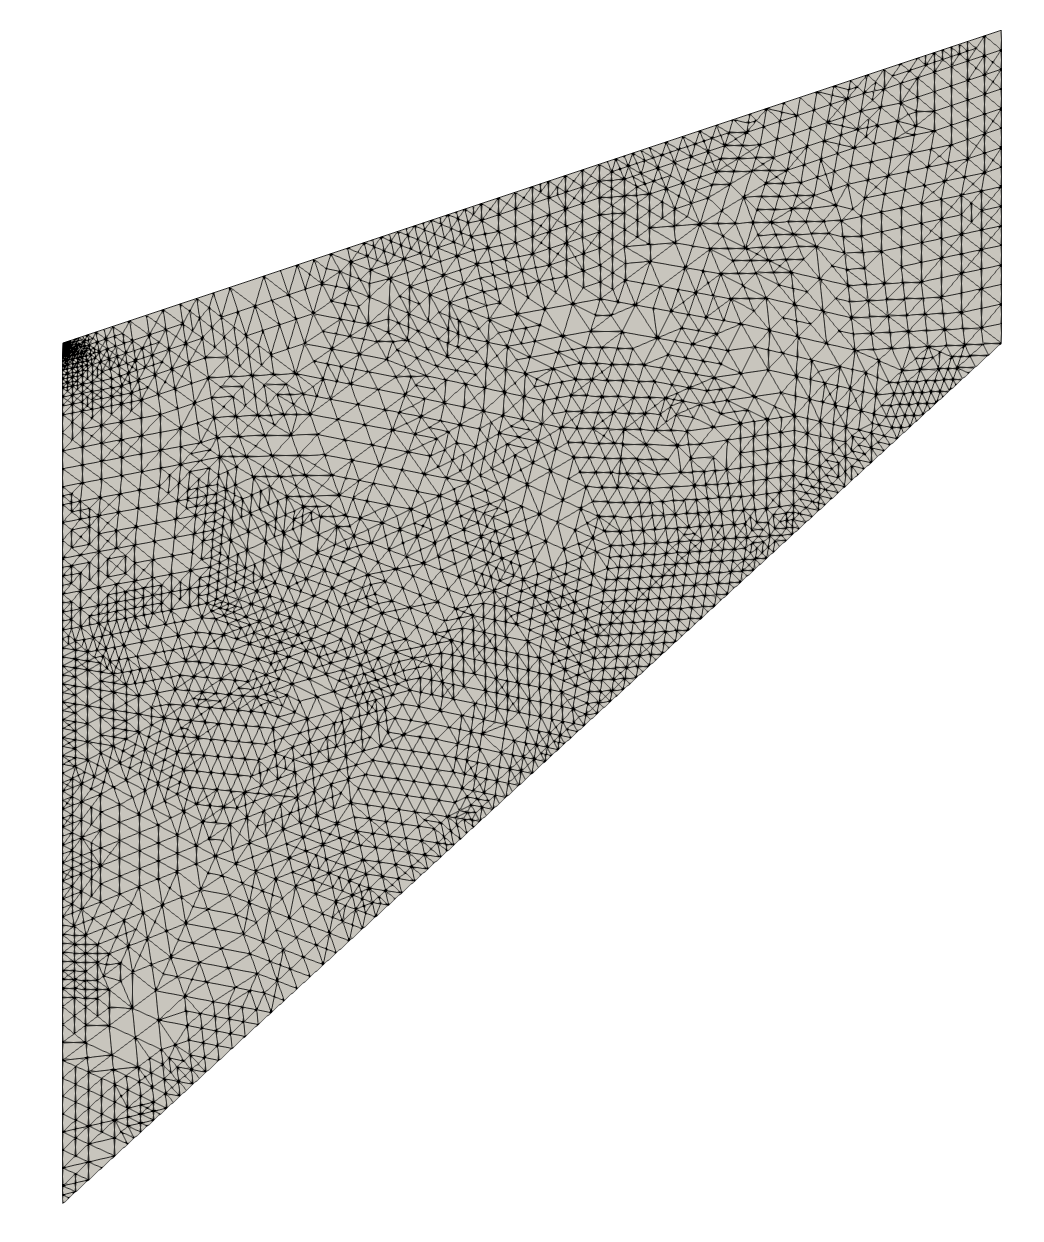
\includegraphics[width=.6\linewidth]{img/mech_cooks_avg_u_final_mesh.png}
\end{subfigure}
\caption{Initial mesh (left) and adapted mesh (right) at the fifth adaptive
iteration for the Cook's membrane problem with the average displacement
QoI $J_2(\bs{U})$.}
\label{fig:mech_cooks_avg_u_meshes}
\end{figure}

We consider two different errors, the ``exact error'' $\E = J(\bs{U}) -
J^h(\bs{U}^h_H)$ and the error $\E_h = J^h(\bs{U}^h) - J^h(\bs{U}^h_H)$
with respect to the functional evaluated on the fine mesh with mesh size
$\frac{H}{2}$. Here we place quotations around the term ``exact error''
because we have only approximated $J(\bs{U})$ with high fidelity and have
not obtained its actual exact value. We recall the effectivity index
\eqref{eq:mech_effectivity} defined as $\I = \frac{\eta}{\E}$ and additionally
define a discrete effectivity index as $I_h = \frac{\eta}{\E_h}$. An
effecitivty index of $\I = 1$ indicates that the error estimate $\eta$ has
exactly recovered the ``true error''. Similarly, a discrete effectivity index
of $\I_h = 1$ indicates that the error estimate $\eta$ has exactly recovered
the error between the functional evaluated on the fine space and the
functional evaluated on the coarse space. Figure
\ref{fig:mech_cooks_effectivity} plots the effectivity $\I$ relative to the
``exact error'' and the effectivity $\I_h$ relative to the fine-space error,
and demonstrates the ability of $\eta$ to effectively estimate the error as
$H \to 0$ during the adaptive process for the chosen functional quantities.
The small distance away from $1$ in the discrete effectivity index $\I_h$
represents the linearization error associated with the estimate $\eta$,
introduced by the linearized adjoint problem \eqref{eq:mech_adjoint_problem}.


\begin{figure}[ht!]
\centering
\begin{subfigure}{.5\textwidth}
\centering
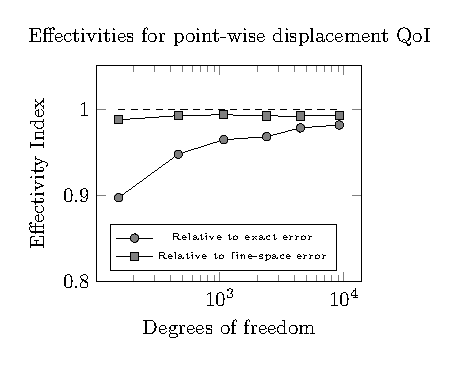
\includegraphics[width=.99\linewidth]{img/mech_cooks_pw_effectivity_plot.pdf}
\end{subfigure}%
\begin{subfigure}{.5\textwidth}
\centering
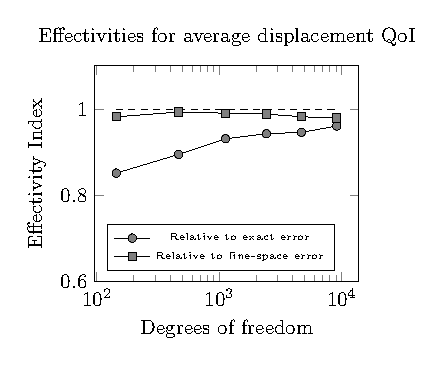
\includegraphics[width=.95\linewidth]{img/mech_cooks_avg_disp_effectivity_plot.pdf}
\end{subfigure}
\caption{Effectivities for the point-wise QoI $J_1(\bs{U})$ (left) and for the
average displacement QoI $J_2(\bs{U})$ (right) for the Cook's membrane
problem.}
\label{fig:mech_cooks_effectivity}
\end{figure}

Figure \ref{fig:mech_cooks_error} demonstrates the evolution of various errors
throughout the adaptive process. First, we note that the ``exact error'' $\E$
and the estimated error $\eta$ are very close, as previously discussed. Next,
we note that the estimated bound $\hat{\eta}$ on the functional error,
computed as the sum of localized error contributions, overestimates the error,
but only by a small factor. This provides some justification to expect that
the derived correction indicators are well-suited to drive mesh adaptation.
Finally, we remark that an improved corrected functional value
$J^*(\bs{U}^h_H)$ can be computed as the approximated functional value plus
the estimated error, $J^*(\bs{U}^h_H) = J^h(\bs{U}^h_H) + \eta$. This
corrected value tends to converge at a faster rate than the computed value
$J^h(\bs{U}^h_H)$. In particular, this corrected value can prove valuable
for coarser discretizations, where the error in the corrected value is
around two orders of magnitude smaller than the error in the computed
value of the functional.

\begin{figure}[ht!]
\centering
\begin{subfigure}{.5\textwidth}
\centering
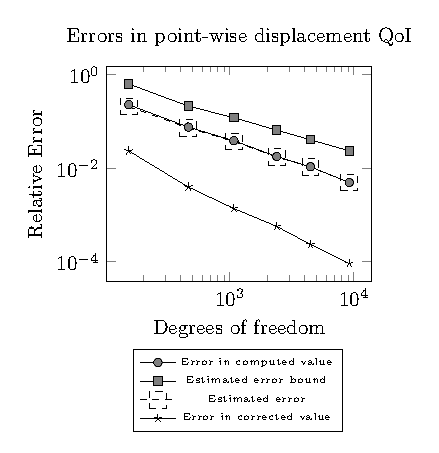
\includegraphics[width=.99\linewidth]{img/mech_cooks_pw_error_plot.pdf}
\end{subfigure}%
\begin{subfigure}{.5\textwidth}
\centering
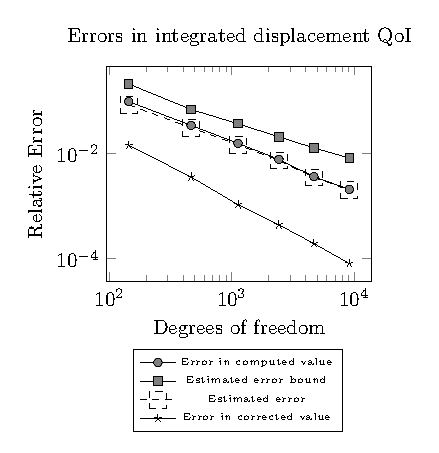
\includegraphics[width=.95\linewidth]{img/mech_cooks_avg_disp_error_plot.pdf}
\end{subfigure}
\caption{Errors for the point-wise QoI $J_1(\bs{U})$ (left) and for the
average displacement QoI $J_2(\bs{U})$ (right) for the Cook' membrane problem.}
\label{fig:mech_cooks_error}
\end{figure}

Figure \ref{fig:mech_cooks_pw_meshes} shows the adapted mesh after $5$
adaptive cycles for the point-wise QoI. We first note that the mesh is
heavily refined in the upper left corner of the mesh, where there is a stress
singularity. Without accurately resolving this singularity, so-called
``pollution error'' \cite{babuvska1994pollution}
will affect the accuracy of the finite element solution
throughout the domain. This demonstrates that the adaptive adjoint-based
procedure accurately identifies other sources of error that must be resolved
even when a fully localized QoI is chosen. Similarly, Figure
\ref{fig:mech_cooks_avg_u_meshes} shows the adapted mesh after $5$
adaptive cycles for the average displacement QoI. Again there is heavy
refinement in the corner with the stress singularity.

Interestingly, Figure \ref{fig:mech_cooks_pw_meshes} also illustrates that
the adjoint-based adaptive procedure refines around the spatial location
that defines the point-wise QoI. This may, in part, be explained by the fact
that the data driving the adjoint problem is a discrete delta function.
However, such refinement is unlikely to lead to an optimal distribution of
degrees of freedom in the mesh. In essence, the Cook's membrane problem
is a cantilever beam and this result indicates that we must refine
heavily at the end of the beam in order to accurately evaluate displacements
at the beam tip. This is antithetical to engineering intuition and
experience. Another factor leading to this result may be our choice of
error localization. We have localized the error based on a PU-based weak
form statement \eqref{eq:mech_error_localization}, where derivatives are left
on the weighting function term $\bs{Z}$. This, in turn, may lead to a
heavier emphasis on the local point-wise location during the adaptive
process. We leave investigation into this area as an avenue for future
study.

%%% A CELL EMBEDDED IN A MATRIX
\subsection{A Cell Embedded in a Matrix}

In this section, we apply adjoint-based error estimation and mesh adaptation
to a three-dimensional problem that arises in the study of cellular
biomechanics and mechanobiology. The problem of interest involves
investigating a cell embedded in an extracellular matrix. The traction that
this cell exerts on its surroundings directly influences cellular processes
like migration and differentiation. Recently, Dong and Oberai
\cite{dong2017recovery} introduced a process to recover cellular tractions
based on the solution of an \emph{inverse} problem. For this inverse problem,
it is assumed that displacements throughout the extracellular matrix are given
with some uncertainty, and successive solutions of a \emph{forward} problem are
solved to recover the tractions driving the problem. Presently, we focus on
accurately solving the forward problem in this process using adjoint-based
error estimation. That is, given tractions imposed on the cellular membrane,
we would like to solve for displacements in some region of the domain as
accurately as possible. 

\begin{figure}[ht!]
\centering
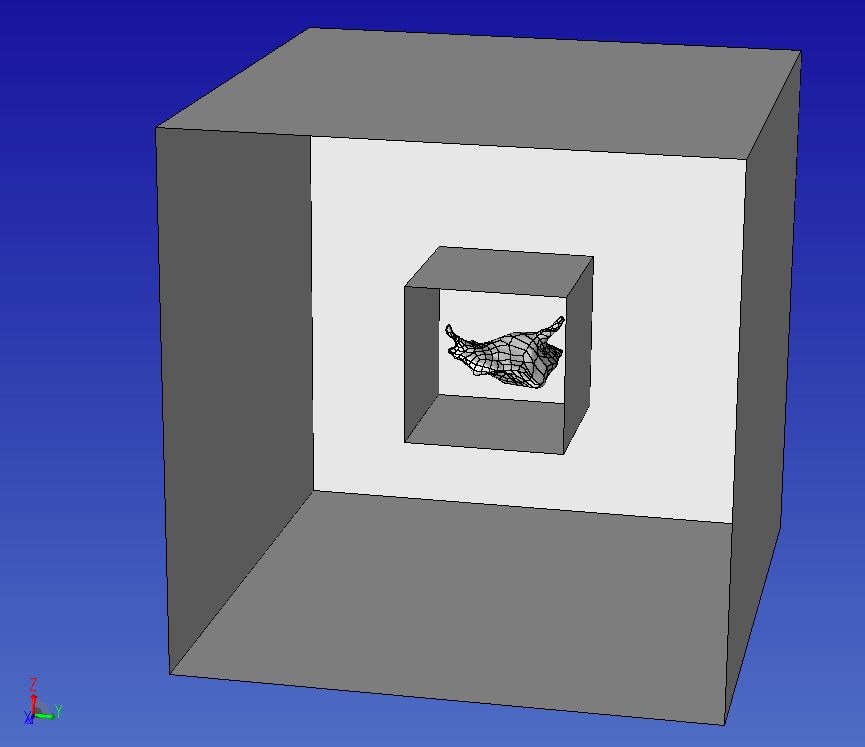
\includegraphics[width=.6\linewidth]{img/mech_glial_geom.png}
\centering
\caption{The computational geometry for the microglial cell problem. The
inner-most surface represents the geometry of the microgial cell, the
outer-most bounding box represents the extracellular matrix in which the
cell is embedded, and the inner bounding box represents the domain over
which the local average displacement QoI $J(\bs{U})$ is defined.}
\label{fig:mech_glial_geom}
\end{figure}

Specifically, we focus on a microglial cell with dimensions of about
$20 \mu m \times 20 \mu m \times 20 \mu m$ embedded in an extracellular matrix
of dimension $100 \mu m \times 100 \mu m \times 100 \mu m$. We choose the
QoI to be a local average displacement,
$J(\bs{U}) = \int_{\B_0} \frac13 (u_x + u_y + u_z) \, \text{d} V$, defined
over a $30 \mu m \times 30 \mu m \times 30 \mu m$ bounding box $\B_0$
surrounding the microglial cell. Figure \ref{fig:mech_glial_geom} shows the
geometry defining the microglial cell, the extracellular matrix, and the
local QoI domain $\B_0$. For the extracellular matrix,
the shear modulus $\mu = \frac{E}{2(1 + \nu)}$ is set to be 600 Pa and
Poisson's ratio is set to be $\nu = 0.4999$, which is consistent with
material properties for hydrogels
\cite{legant2010measurement, paszek2005tensional, discher2005tissue}.

\begin{figure}[ht!]
\centering
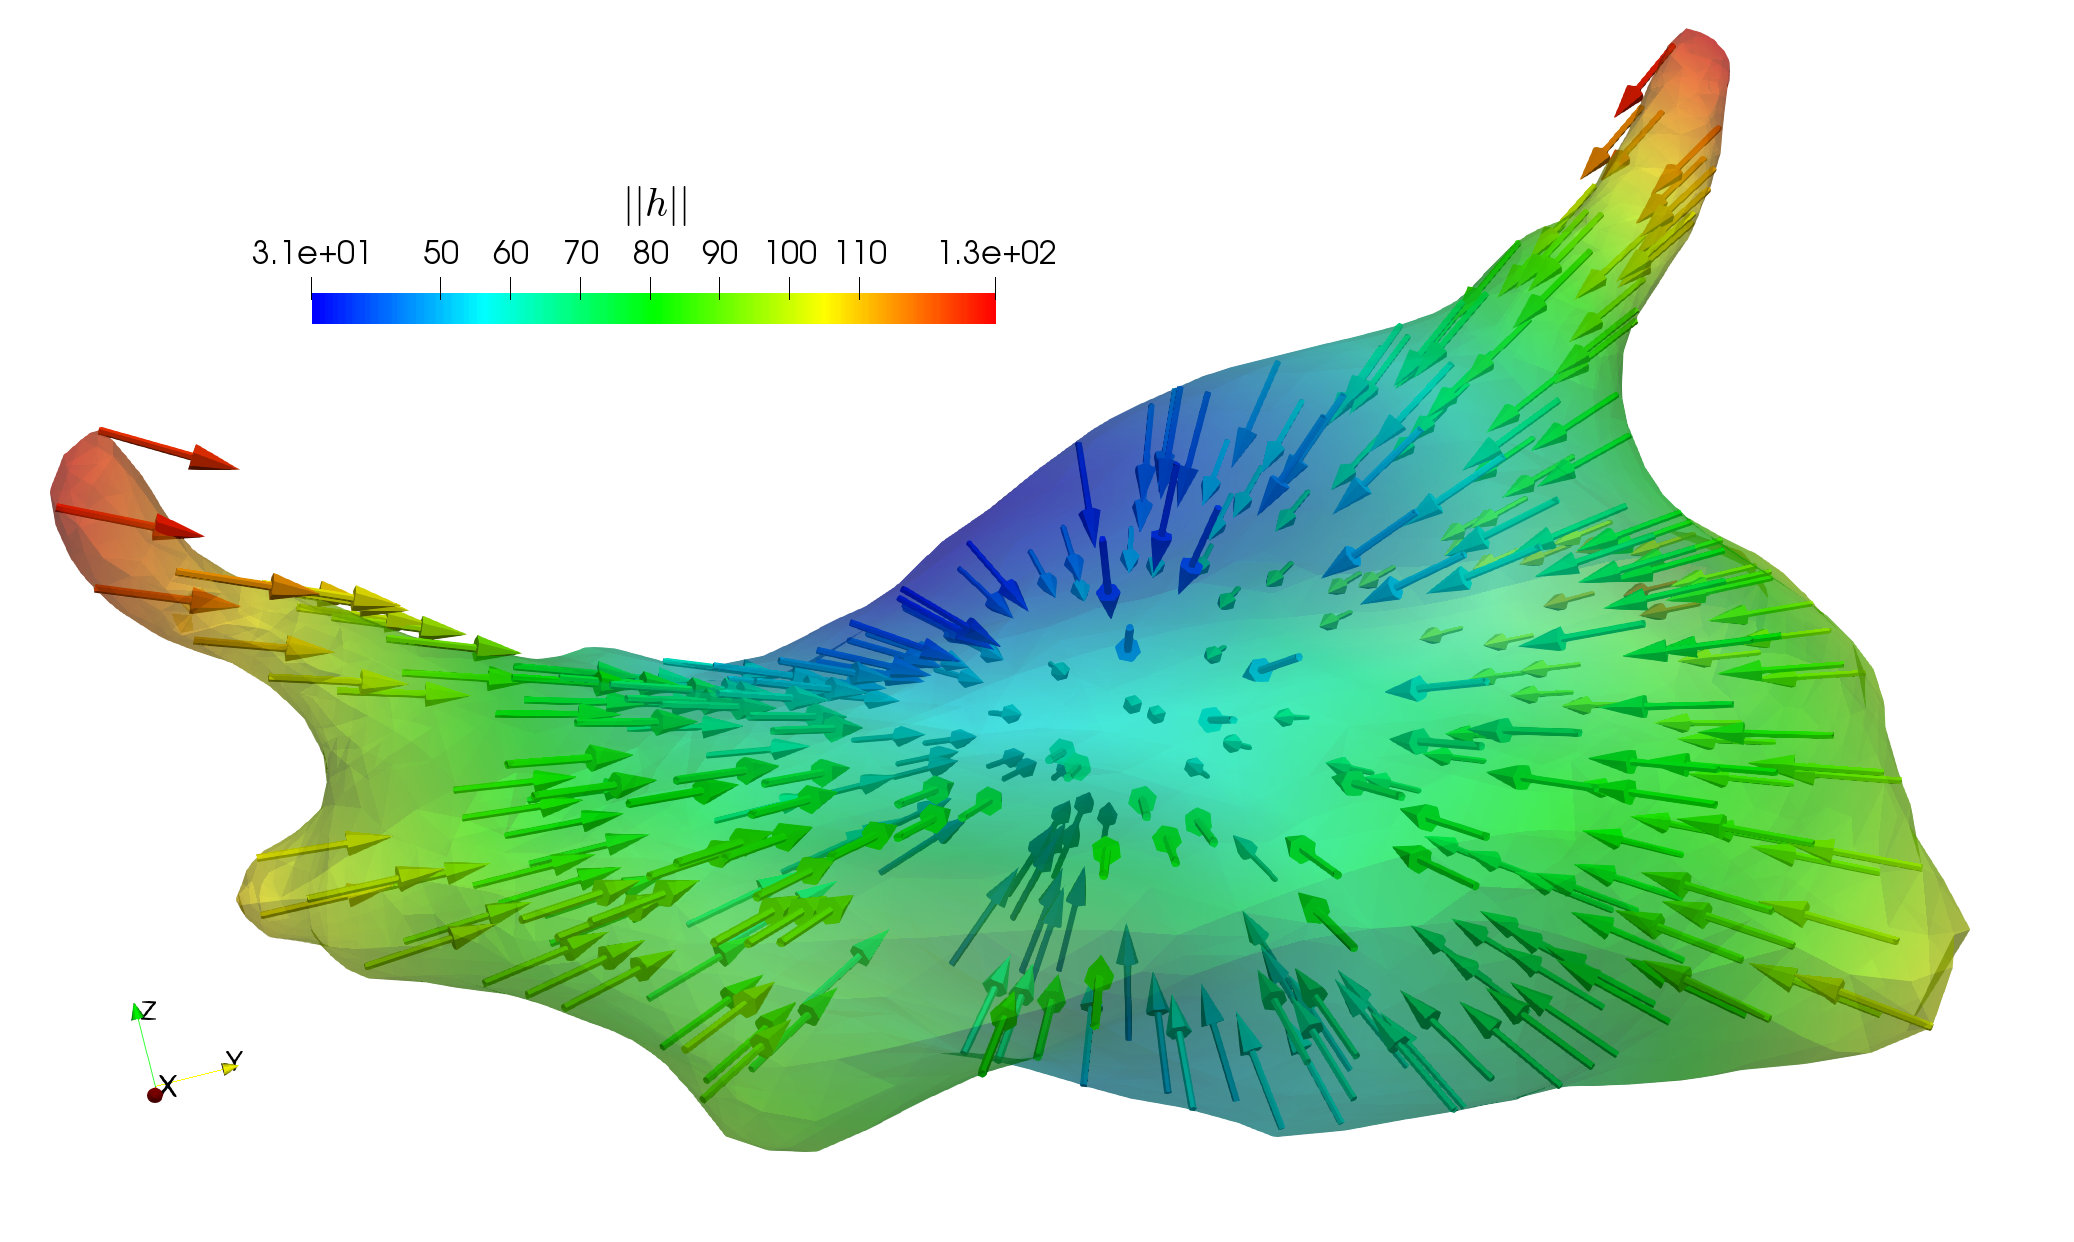
\includegraphics[width=.6\linewidth]{img/mech_glial_applied_traction.png}
\centering
\caption{The applied tractions for the microglial cell problem.}
\label{fig:mech_glial_traction}
\end{figure}

To drive the problem, we impose traction boundary conditions along the
surface of the microglial cell. The magnitude of the traction $\bs{h}$ is
defined to be 10 times the distance to the center of the microglial cell and
its direction points inward toward the center of the microglial cell. The
applied traction is shown in Figure \ref{fig:mech_glial_traction}. This
traction serves to pull the extracellular matrix inwards towards the center
of the microglial cell, which is consistent with observed physical behavior
\cite{dong2017recovery}. The deformation of the cell surface due to this
applied traction is shown in Figure \ref{fig:mech_glial_deformed}. To
constrain rigid body translations and rotations, we prescribe displacements
$u_x = 0$ on the face with constant minimum $x$-coordinate value, $u_y = 0$
on the face with constant minimum $y$-coordinate value, and $u_z = 0$ on the
face with constant minimum $z$-coordinate value. As a reference value for
the average displacement QoI, the primal problem was solved on a ``truth''
mesh with about $60$ million degrees of freedom. The reference value for the
QoI was computed to be $J(\bs{U}) = -527.1453$.

\begin{figure}[ht!]
\centering
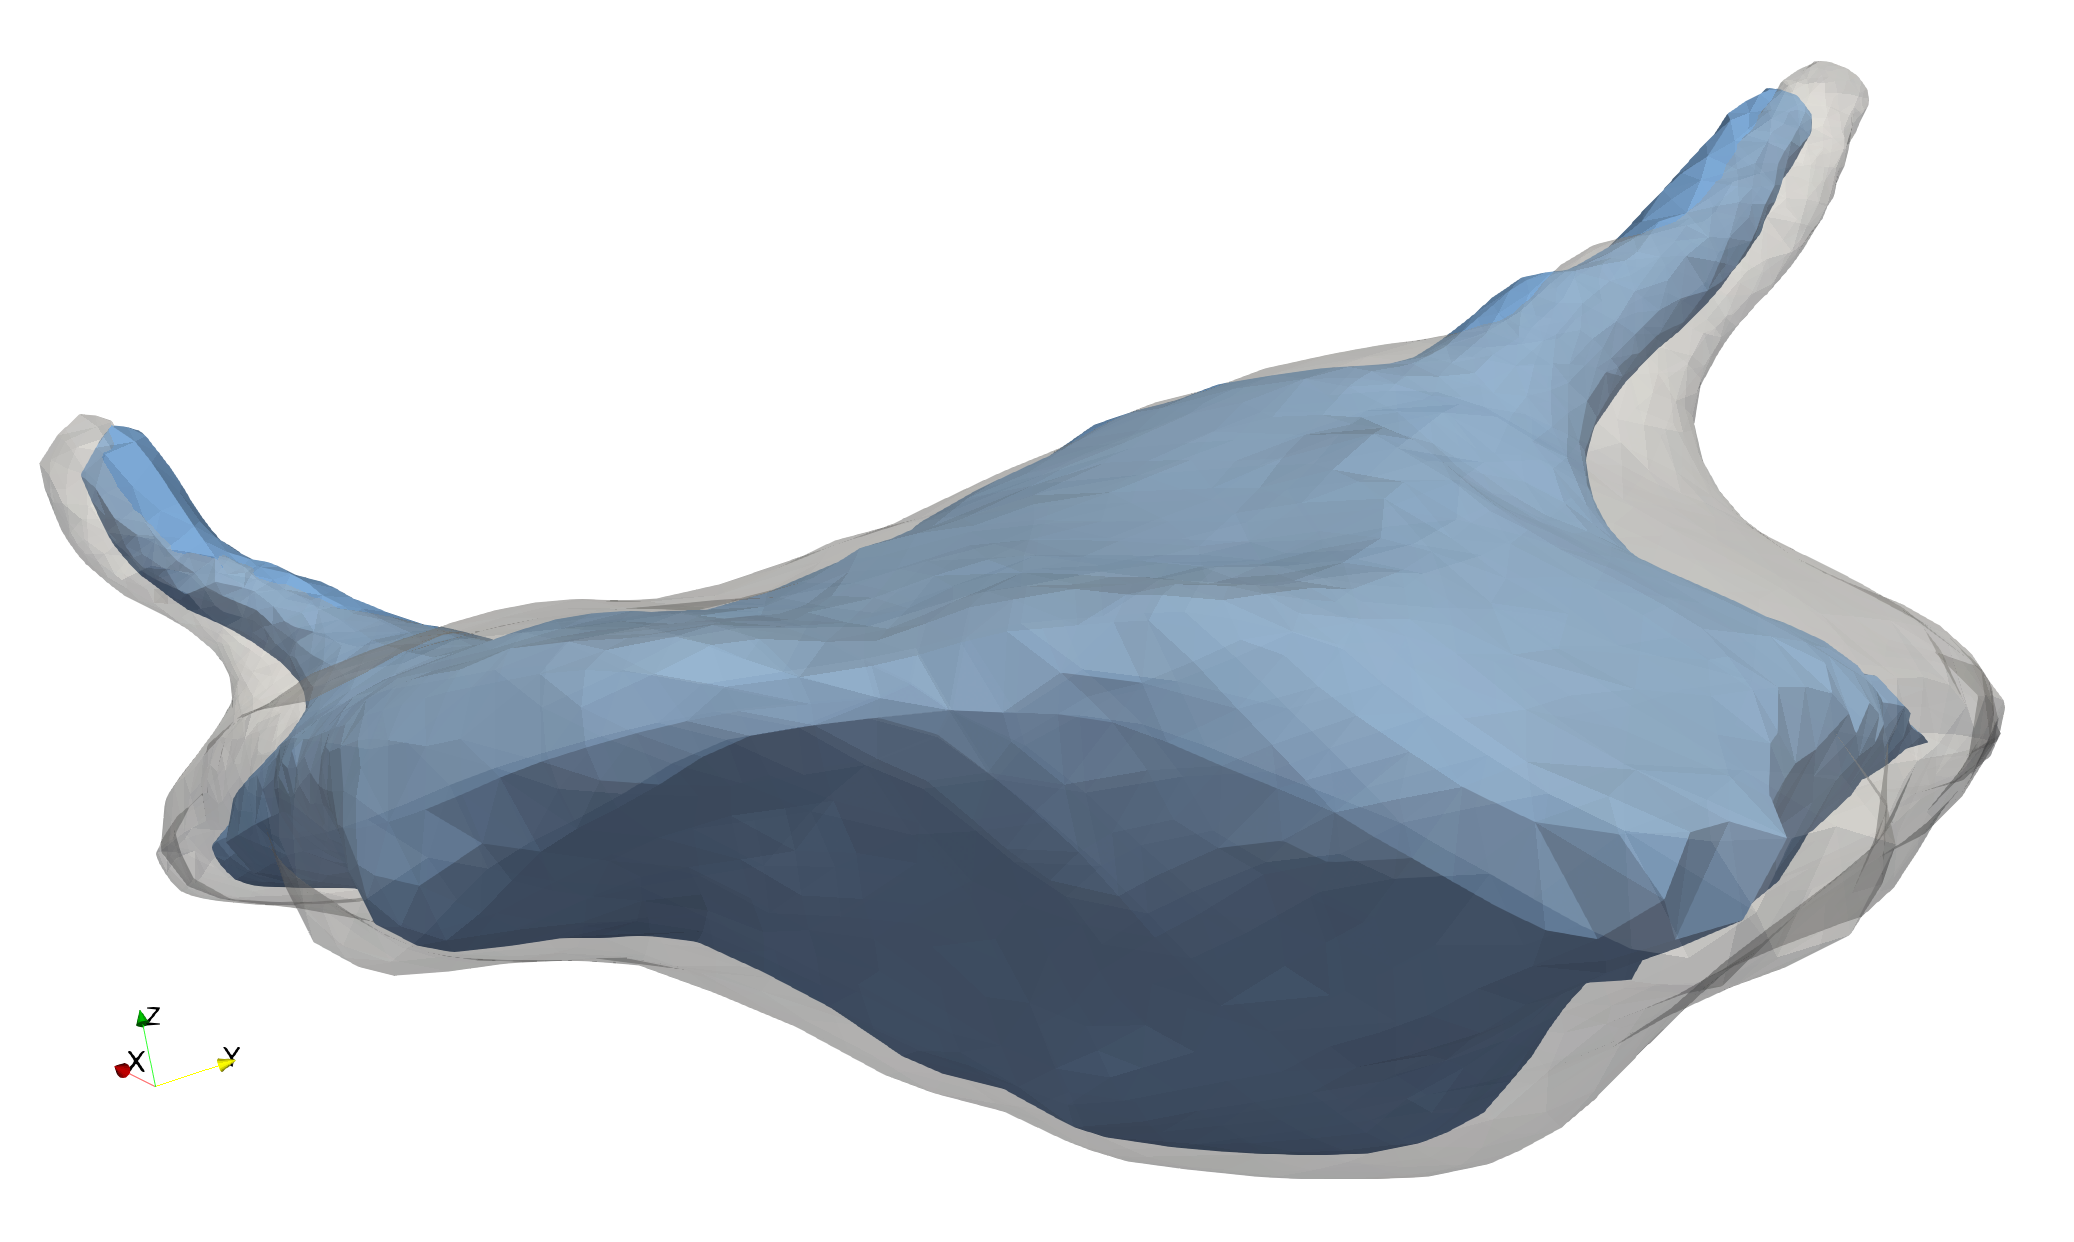
\includegraphics[width=.6\linewidth]{img/mech_glial_deformed.png}
\caption{The initial (light grey) and deformed (blue) geometry of the
microglial cell before and after tractions are applied.}
\label{fig:mech_glial_deformed}
\end{figure}

\begin{figure}[ht!]
\centering
\begin{subfigure}{.5\textwidth}
\centering
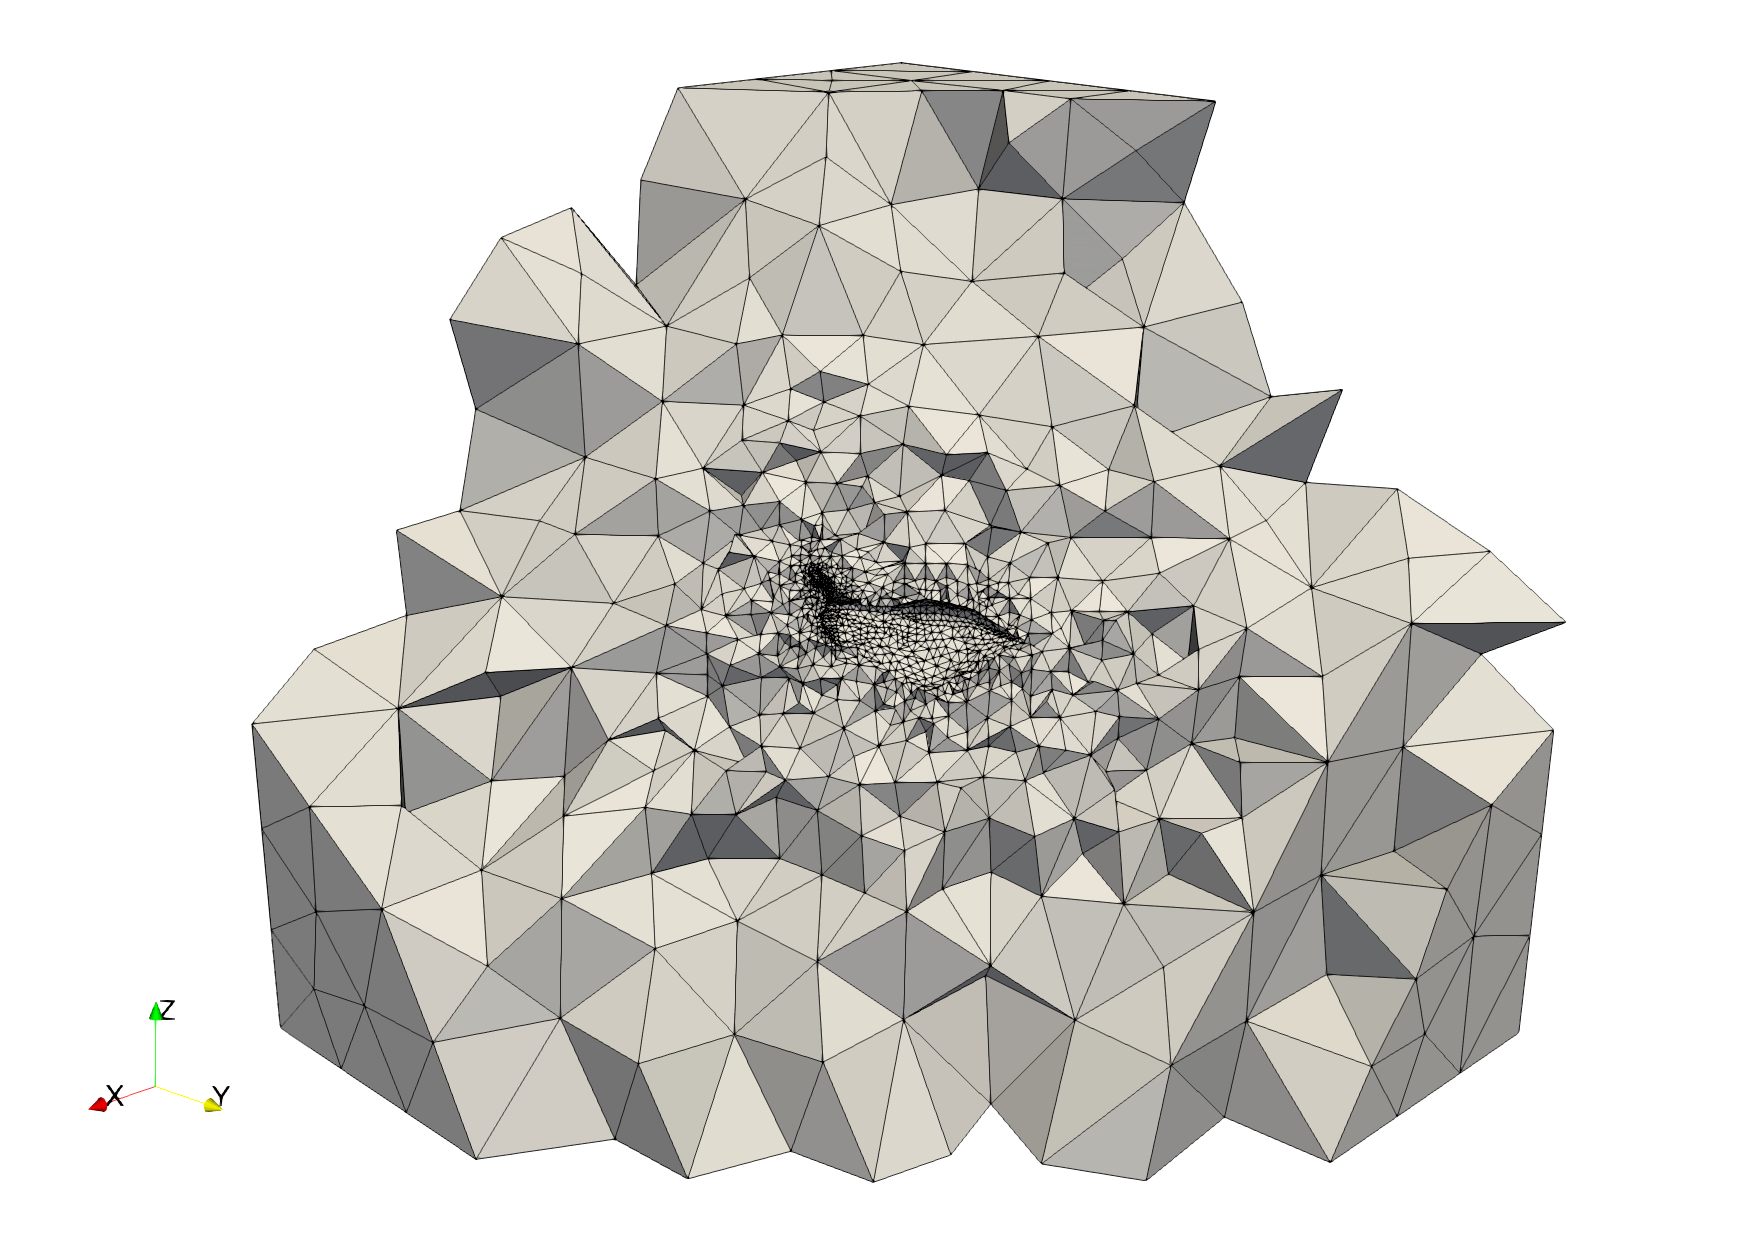
\includegraphics[width=.99\linewidth]{img/mech_glial_initial_mesh.png}
\end{subfigure}%
\begin{subfigure}{.5\textwidth}
\centering
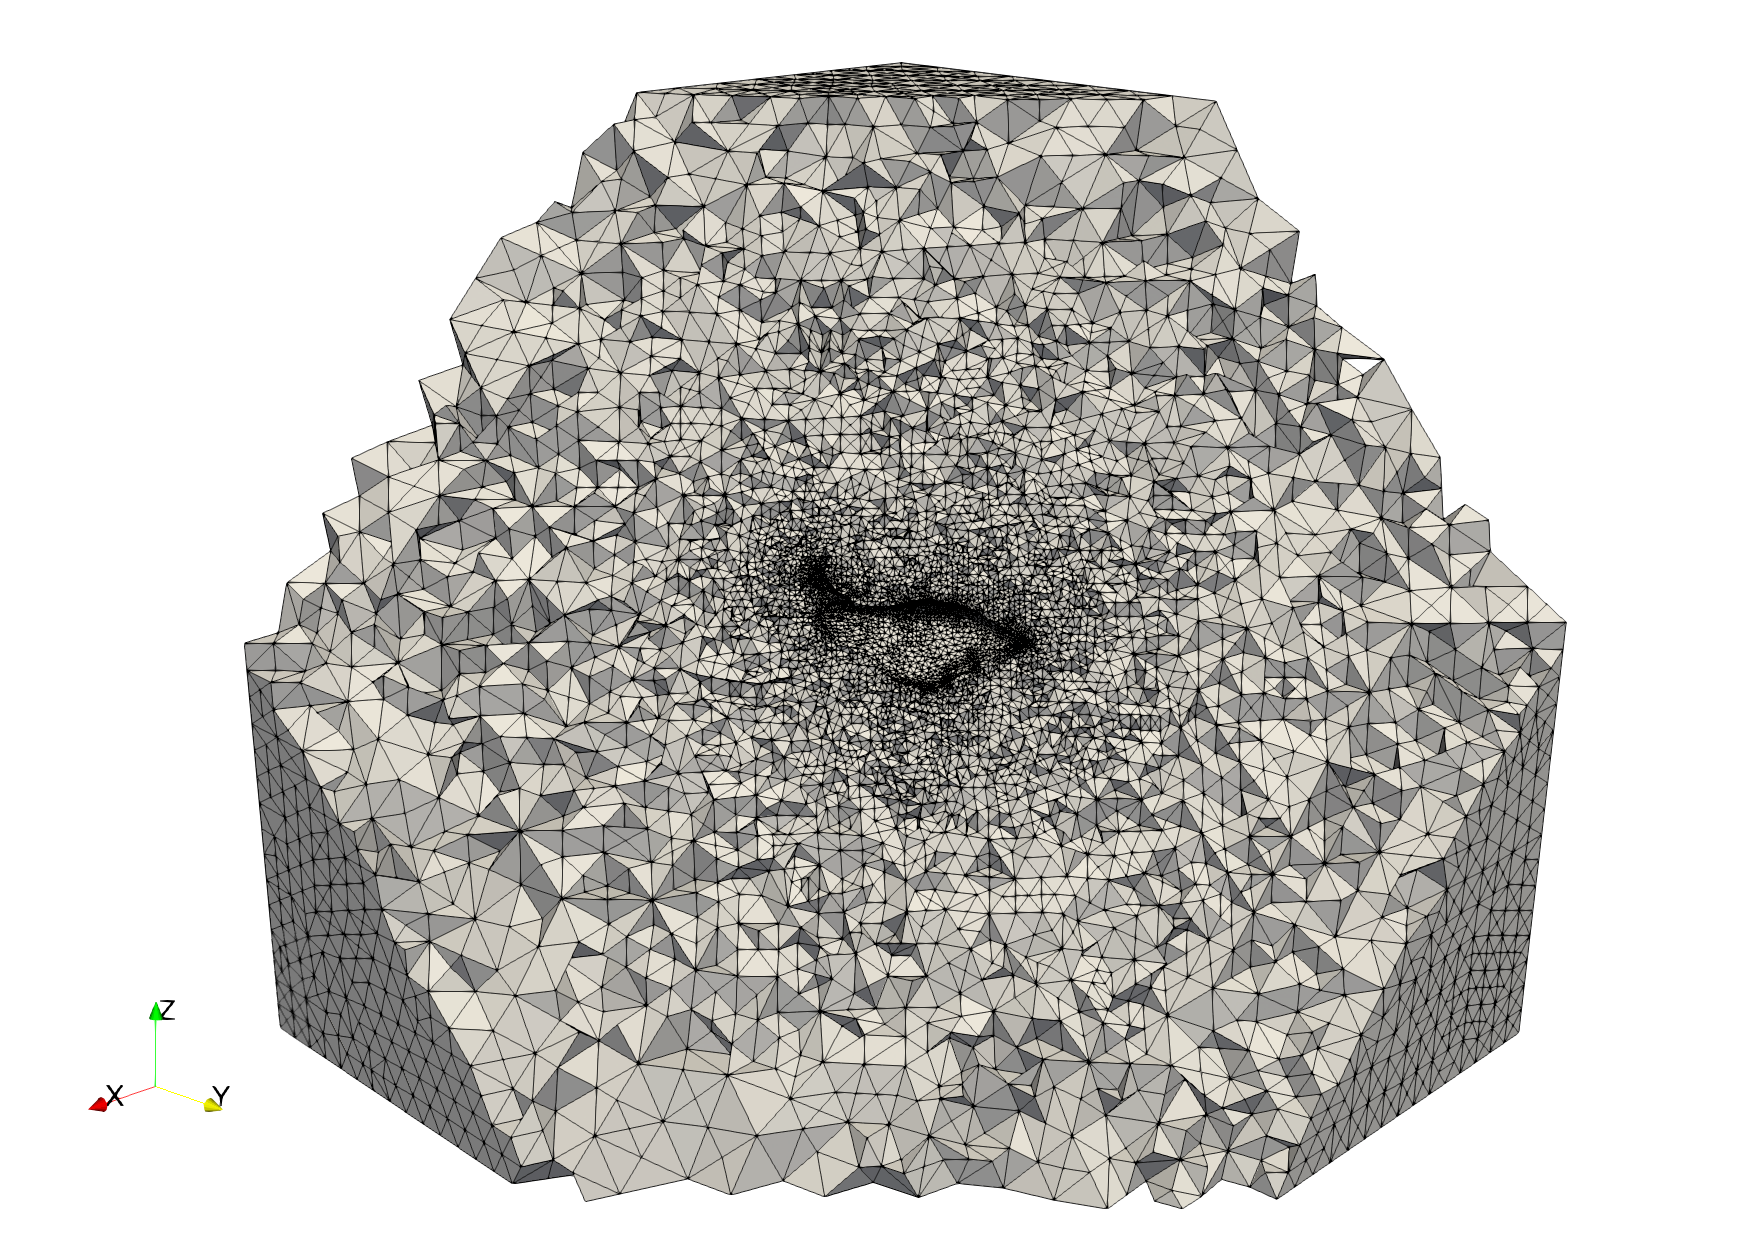
\includegraphics[width=.99\linewidth]{img/mech_glial_final_mesh.png}
\end{subfigure}
\caption{Initial mesh for the microglial cell problem (left) and final adapted
mesh after $10$ adaptive iterations (right).}
\label{fig:mech_glial_meshes}
\end{figure}

An initial mesh with about $30,000$ degrees of freedom was generated, as
shown in Figure \ref{fig:mech_glial_meshes}. From this initial mesh, the
steps
%
\begin{gather*}
\text{Solve primal PDE} \rightarrow
\text{Solve adjoint PDE} \rightarrow
\text{Localize error} \rightarrow
\text{Adapt mesh}
\end{gather*}
%
were iteratively performed $10$ times.  The mesh size field was specified
according to equation \eqref{eq:mech_size_field} such that the desired number
of elements $N$ in the output mesh is $1.5$ times the number of elements in
the previous mesh.

\begin{figure}[ht!]
\centering
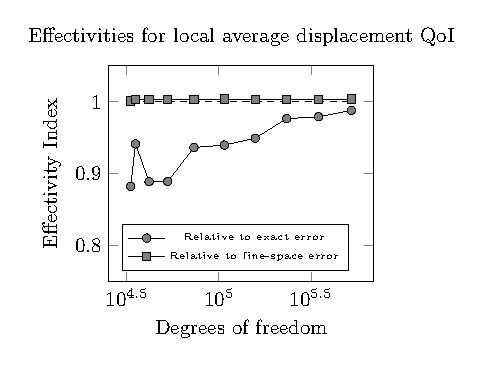
\includegraphics[width=.5\linewidth]{img/mech_glial_effectivity_plot.pdf}
\caption{Effectivity indices for the local average displacement QoI
$J(\bs{U})$ for the microglial cell problem.}
\label{fig:mech_glial_effectivity}
\end{figure}

We again consider the ``exact error'' $\E = J(\bs{U}) - J^h(\bs{U}^h_H)$ and
the error $\E_h = J^h(\bs{U}^h) - J^h(\bs{U}^h_H)$ with respect to the
functional evaluated on the fine mesh, and their effectivity indices
$\I = \frac{\eta}{\E}$ and $I_h = \frac{\eta}{\E_h}$, respectively. Here
$\eta$ denotes the error estimate computed by \eqref{eq:mech_error_estimate}.
We again expect that the functional will converge at the rate $k = 2$ and use
the correction value $\alpha = \frac34$.

Figure \ref{fig:mech_glial_effectivity} plots the effectivity index $\I$
relative to the ``exact error'' and the effectivity index $I_h$ relative to the
fine space error. The small distance away from $1$ in the discrete effectivity
index $\I_h$ is associated with the linearization error introduced by the
adjoint problem. Additionally, the ability of the error estimate to recover
the ``exact error'' as $H \to 0$ compared to the reference value is
demonstrated by the effectivity $\I$.

\begin{figure}[ht!]
\centering
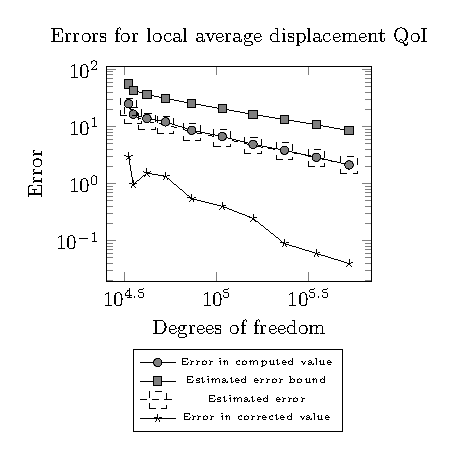
\includegraphics[width=.5\linewidth]{img/mech_glial_error_plot.pdf}
\caption{Errors for the local average displacement QoI $J(\bs{U})$ for the
microglial cell problem.}
\label{fig:mech_glial_error}
\end{figure}

\begin{figure}[ht!]
\centering
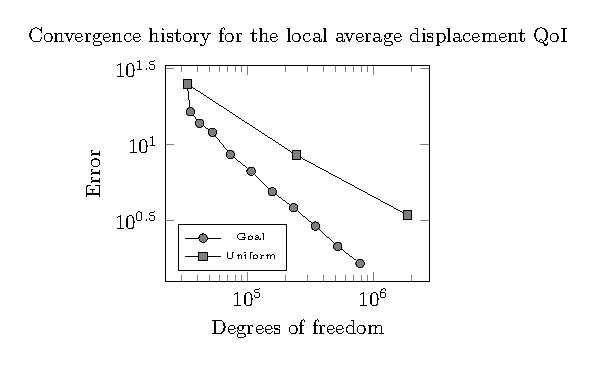
\includegraphics[width=.6\linewidth]{img/mech_glial_convergence_plot}
\caption{Error convergence using uniform mesh refinement (Uniform) and
adjoint-based adaptivity (Goal) for the local average displacement QoI
$J(\bs{U})$ for the microglial cell problem.}
\label{fig:mech_glial_convergence}
\end{figure}

Figure \ref{fig:mech_glial_error} displays the evolution of various errors
throughout the adaptive process. In particular, the ``exact error'' $\E$ and
the estimated error $\eta$ are very close, as previously noted by the
effectivity index $\I$. As for the Cook's membrane problem the estimated error
bound $\hat{\eta}$ overestimates the error, but not to a drastic degree.
Finally, we remark that the corrected functional value, computed as
$J^*(\bs{U}^h_H) = J^h(\bs{U}^h_H) + \eta$, is nearly two orders of magnitude
more accurate at the final adaptive step, demonstrating the usefulness
of adjoint-based error estimation.

Finally, we plot the evolution of the ``exact error'' for two adaptive
strategies in Figure \ref{fig:mech_glial_convergence}. We compare the
convergence of errors for uniform mesh refinement and the developed
adjoint-based adaptive scheme. The error is converging at a faster rate for
the adjoint-based adaptive scheme. Further, the adjoint-based adaptive scheme
achieves the same accuracy as the uniform refinement scheme with nearly an
order of magnitude fewer degrees of freedom at around $110,000$ degrees
freedom. This demonstrates the utility of adjoint-based adaptivity for solid
mechanics problems.

%%% CONCLUSIONS
\section{Conclusions}

In this chapter, we have developed an adjoint-based error estimation
procedure for nonlinear finite deformation elasticity using a stabilized
finite element method, where we have utilized a recently developed PU-based
error localization strategy. We have demonstrated the ability of this approach
to accurately estimate functional errors for a two-dimensional model
problem. Further, we have demonstrated the utility of adaptive adjoint-based
analysis in the context of a three-dimensional example problem motivated
by the study of biological tissues. Future work includes analytically and
numerically investigating the differences in the PU-based localization
approach as compared to a more classical strong-form localization approach
for localized point-wise quantities of interest.

\chapter{A NON-UNIFORM REFINEMENT APPROACH
FOR SOLVING ADJOINT PROBLEMS IN FUNCTIONAL
ERROR ESTIMATION AND MESH ADAPTATION}
\label{chap:refine}

%%% INTRODUCTION
\section{Introduction}

Adjoint-based error estimation
\cite{becker2001optimal, giles2003adjoint,
pierce2004adjoint, venditti2000adjoint,
venditti2002adjoint,
venditti2003adjoint,
prudhomme1999goal,
prudhomme2003practical,
fidkowski2011review,
connors2013method}
is a tool used in numerical simulation
to estimate the discretization error
in physically meaningful output quantities.
Combined with mesh adaptation, adjoint-based error
estimation also provides the ability to control the discretization
error. The process of adjoint-based error estimation
relies on the introduction of an auxiliary
\emph{adjoint problem}, which is constructed using
the solution to the original or \emph{primal problem}
of interest.

To obtain meaningful error estimates,
the solution to the adjoint problem must be
enriched in some manner. That is, it is
necessary to obtain a representation of the
adjoint solution in a richer space compared
to the space used for the primal problem.
Several strategies are commonly
to obtain an enriched adjoint representation.
These approaches include
solving the adjoint problem in a globally higher
order polynomial space
\cite{fidkowski2011output},
solving the adjoint problem on a uniformly
refined mesh \cite{burstedde2009parallel},
solving the adjoint problem in the same space
as used for the primal problem
and solving local patch-wise problems least
squares problems \cite{nemec2007adjoint} or
by performing patch-wise higher-order interpolation
\cite{becker2001optimal},
and enriching the adjoint solution via
variational multiscale methods
\cite{granzow2017output}.

Solving the adjoint problem in a globally higher
order polynomial or on a uniformly refined mesh
is a computationally expensive proposition. On the
other hand, solving the adjoint problem in the same
space as used for the primal problem and enriching
it via local patch-wise problems may not be guaranteed
to yield a more accurate adjoint solution. In this
chapter, we propose a simple compromise and solve the
adjoint problem on meshes obtained via non-uniform
refinement.

The remainder of this chapter is structured as follows.
First, we review adjoint-based error estimation for
functional quantities using two discretization levels,
a \emph{coarse} space and a \emph{fine} space. We then
review three choices for the fine space, obtained
by refinement of the mesh used for the coarse space.
The first choice is the standard uniform refinement
method, while the other two approaches form the fine
space via non-uniform refinement. In each of these
sections, we discuss the algorithm utilized to generate
the fine space. We then investigate the these three
approaches for adjoint enrichment for Poisson's equation
and conclude with a summary of the results.

%%% OUTPUT ERROR ESTIMATION WITH TWO DISCRETIZATION LEVELS
\section{Error Estimation with Two Levels}

\subsection{Error Estimates}

Let $\V^h$ and $\V^H$ denote finite dimensional spaces
such that $\V^H \subset \V^h$. We refer to $\V^h$
and $V^H$ as the \emph{fine} space and the \emph{coarse}
space, respectively. Let $\bs{R}^H : \mathbb{R}^N \to \mathbb{R}^N$
denote the system of (potentially nonlinear) algebraic equations
arising from a finite element discretization of a PDE on the
coarse space $\V^H$, such that the solution vector
$\bs{u}^H \in \mathbb{R}^N$ satisfies
%
\begin{gather}
\bs{R}^H(\bs{u}^H) = 0.
\label{eq:refine_residual_coarse}
\end{gather}
%
Similarly, let $\bs{R}^h : \mathbb{R}^n \to \mathbb{R}^n$
denote the system of algebraic equations arising from a finite
element discretization of the same PDE on the fine space
$\V^h$, such that
%
\begin{gather}
\bs{R}^h(\bs{u}^h) = 0,
\label{eq:refine_residual_fine}
\end{gather}
%
where $\bs{u}^h \in \mathbb{R}^n$ is the solution vector on
the fine space and $n > N$.

Let $J^H : \mathbb{R}^N \to \mathbb{R}$ denote a discrete
representation of a physically meaningful functional quantity
on the coarse space $\V^H$, and similarly let
$J^h : \mathbb{R}^n \to \mathbb{R}$ denote the functional
approximated on the fine space $\V^h$. Let
$\bs{u}^h_H := \bs{I}^h_H \bs{u}^H$ denote the prolongation of
the coarse space solution $\bs{u}^H$ onto the fine space
$\V^h$ via interpolation, where
$\bs{I}^h_H : \V^H \to \V^h$.

The functional evaluated on the fine space $J(\bs{u}^h)$
can be expanded in a Taylor series approximation about the
prolonged coarse space solution $\bs{u}^h_H$ as
%
\begin{gather}
J^h(\bs{u}^h) = J^h(\bs{u}^h_H) +
\left[ \frac{\partial J^h}{\partial \bs{u}^h}
\biggr|_{\bs{u}^h_H} \right]
(\bs{u}^h - \bs{u}^h_H) + \dots
\label{eq:refine_functional_taylor}
\end{gather}
%
Similarly, the residual system of equations evaluated
on the fine space $\bs{R}^h(\bs{u}^h)$ can be expanded
about the prolonged coarse space solution $\bs{u}^h_H$ as
%
\begin{gather}
\bs{R}^h(\bs{u}^h) = \bs{R}^h(\bs{u}^h_H) +
\left[ \frac{\partial \bs{R}^h}{\partial \bs{u}^h}
\biggr|_{\bs{u}^h_H} \right]
(\bs{u}^h - \bs{u}^h_H) + \dots
\label{eq:refine_residual_taylor}
\end{gather}
%
Using the governing relation \eqref{eq:refine_residual_fine} in the
residual Taylor expansion \eqref{eq:refine_residual_taylor} suggests
a first order approximation for the discretization error between the
spaces:
%
\begin{gather}
(\bs{u}^h - \bs{u}^h_H) \approx
- \left[ \frac{\partial \bs{R}^h}{\partial \bs{u}^h}
\biggr|_{\bs{u}^h_H} \right]^{-1}
\bs{R}^h(\bs{u}^h_H).
\label{eq:refine_disc_error_approx}
\end{gather}
%
Inserting the error approximation \eqref{eq:refine_disc_error_approx}
into the functional Taylor expansion \eqref{eq:refine_functional_taylor}
suggests the error estimate:
%
\begin{gather}
J^h(\bs{u}^h) - J^h(\bs{u}^h_H) \approx
- \left[ \frac{\partial J^h}{\partial \bs{u}^h}
\biggr|_{\bs{u}^h_H} \right]
\left[ \frac{\partial \bs{R}^h}{\partial \bs{u}^h}
\biggr|_{\bs{u}^h_H} \right]^{-1}
\bs{R}^h(\bs{u}^h_H),
\end{gather}
%
which can be re-written in terms of an \emph{adjoint} variable
$\bs{z}^h$ as
%
\begin{gather}
J^h(\bs{u}^h) - J^h(\bs{u}^h_H) \approx
- \bs{z}^h \cdot \bs{R}^h (\bs{u}^h_H),
\label{eq:refine_adjoint_error}
\end{gather}
%
where $\bs{z}^h \in \mathbb{R}^n$ is the solution to the
so-called \emph{adjoint problem} given by
%
\begin{gather}
\left[ \frac{\partial \bs{R}^h}{\partial \bs{u}^h}
\biggr|_{\bs{u}^h_H} \right]^T
\bs{z}^h
=
- \left[ \frac{\partial J^h}{\partial \bs{u}^h}
\biggr|_{\bs{u}^h_H} \right]^T.
\label{eq:refine_adjoint_problem}
\end{gather}

\subsection{A Simple a-priori Analysis}

Consider that the functional of interest
converges at the rate $k$, such that
$J - J^h(\bs{u}^h_H) = c H^k$ and
$J - J^h(\bs{u}^h) = c h^k$,
where $J$ is the exact value of the functional
quantity of interest. Assume that the fine space
is obtained via refinement of the coarse space.
Consider the ratio
%
\begin{gather}
\frac{J^h(\bs{u}^h) - J^h(\bs{u}^h_H)}
{J - J^h(\bs{u}^h_H)} \approx
\frac{ - \bs{z}^h \cdot \bs{R}^h(\bs{u}^h_H)}
{J - J^h(\bs{u}^h_H)}
\end{gather}
%
which, as $H \to 0$, will tend towards \cite{fidkowski2011review}
%
%% refine_alpha
\begin{gather}
\alpha := 1 - \left( \frac{h}{H} \right)^k.
\label{eq:refine_alpha}
\end{gather}
%

Let $\eta$ denote our approximation to the
functional error $J - J^h(\bs{u}^h_H)$.
Let $\I$ denote the effectivity index
given by
%
\begin{gather}
\I = \frac{\eta}{J - J^h(\bs{u}^h_H)}.
\label{eq:refine_effectivity}
\end{gather}
%
We would like error estimates
$\E$ that lead to effectivity indices of
$\I = 1$ as $H \to 0$. To achieve this, we scale
the two-level adjoint weighted residual estimate
\eqref{eq:refine_adjoint_error} by the inverse
of the factor $\alpha$, such that
%
\begin{gather}
\eta = - \frac{1}{\alpha}
\bs{z}^h \cdot \bs{R}^h(\bs{u^h_H})
\label{eq:refine_error_approx}
\end{gather}

%%% CHOICES FOR THE FINE SPACE
\section{Choices for the fine space}

%%% UNIFORM REFINEMENT
\subsection{Uniform Refinement}

\begin{figure}[ht!]
\centering
\begin{subfigure}{.5\textwidth}
\centering
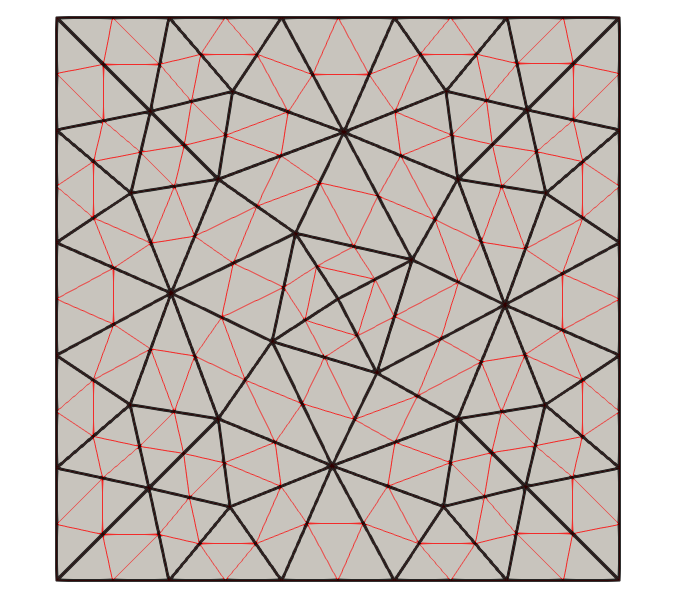
\includegraphics[width=.9\linewidth]{img/refine_unif_mesh.png}
\end{subfigure}%
\begin{subfigure}{.5\textwidth}
\centering
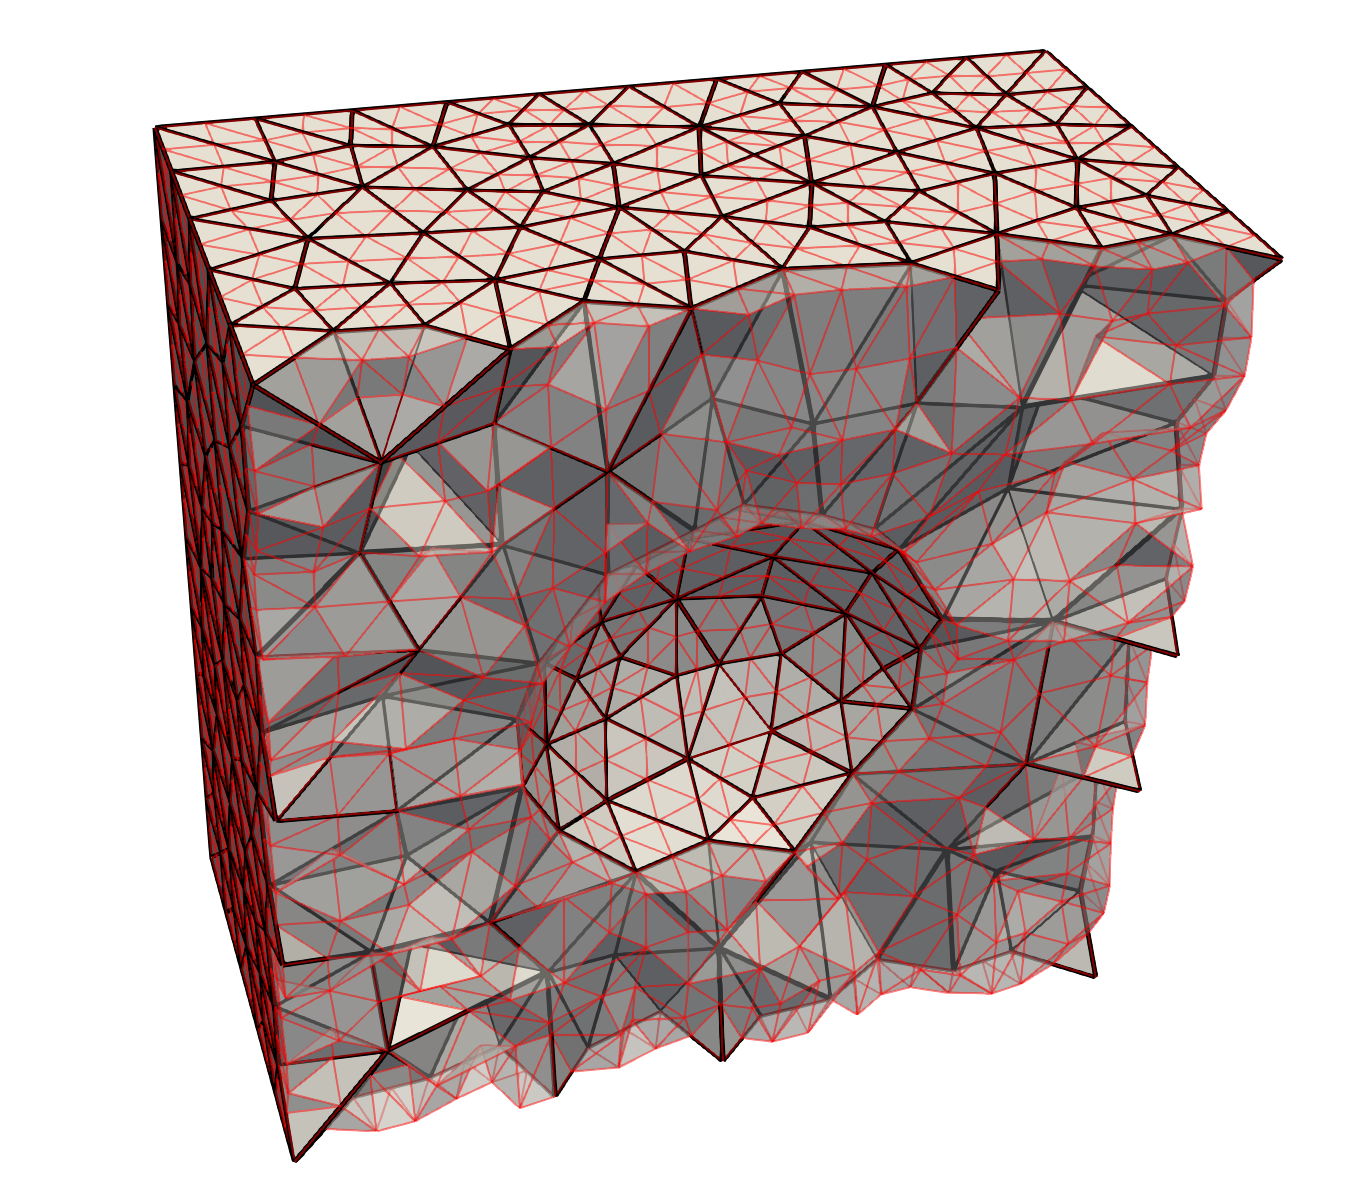
\includegraphics[width=.99\linewidth]{img/refine_unif_mesh_3D.png}
\end{subfigure}
\caption{Edges of a base mesh (black) and a nested mesh refined
with the Unif scheme (red) in two dimensions.}
\label{fig:unif_mesh}
\end{figure}

We first consider the traditional approach of using
a uniformly refined mesh to solve the adjoint problem.
We refer to this approach as the \textsc{Unif}
refinement approach.
To perform uniform refinement, every edge in the mesh
is marked for refinement. The algorithm for uniform
refinement is given in Algorithm \ref{alg:uniform_refine}.
Figure \ref{fig:unif_mesh} demonstrates an example of the
\textsc{Unif} refinement approach applied to a
base mesh. For the uniform refinement approach,
we naturally choose the ration $\frac{h}{H} = \frac12$,
leading to the scaling parameter
$\alpha = 1 - \left( \frac12 \right)^k.$

\begin{algorithm}
\caption{Uniform refinement algorithm}
\begin{algorithmic}
\For{ each edge $e$ in mesh $M$ }
\State mark edge $e$ for refinement.
\EndFor
\end{algorithmic}
\label{alg:uniform_refine}
\end{algorithm}

%%% LONG EDGE REFINEMENT
\subsection{Long Edge Refinement}

\begin{figure}[ht!]
\centering
\begin{subfigure}{.5\textwidth}
\centering
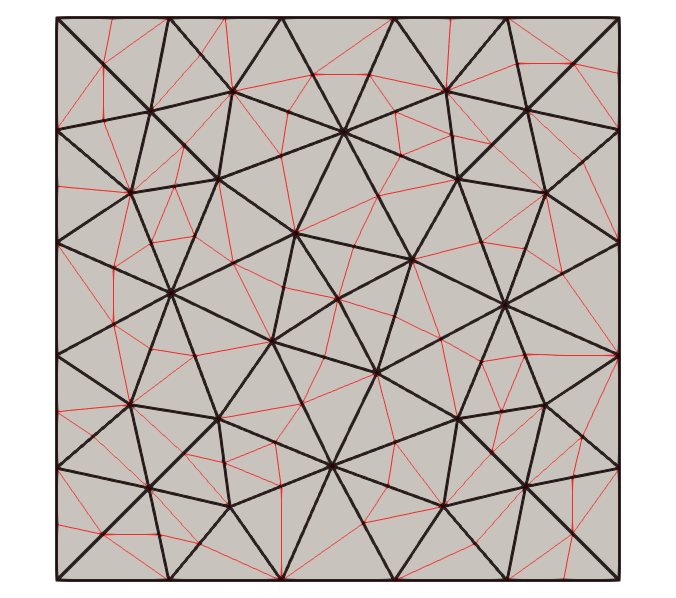
\includegraphics[width=.9\linewidth]{img/refine_long_mesh.png}
\end{subfigure}%
\begin{subfigure}{.5\textwidth}
\centering
\includegraphics[width=.99\linewidth]{img/refine_long_mesh_3D.png}
\end{subfigure}
\caption{Edges of a base mesh (black) and a nested mesh refined
with the Long scheme (red) in two dimensions.}
\label{fig:long_mesh}
\end{figure}

Next, we consider an adaptive scheme that marks
the longest edge in each element for refinement.
We refer to this scheme as the Long edge
refinement scheme. The \textsc{Long} edge refinement
algorithm is outlined in Algorithm \ref{alg:long_refine}.
Figure \ref{fig:long_mesh} illustrates the
\textsc{Long} edge refinement algorithm applied to
a base mesh.

Not that, for the \textsc{Long} edge refinement
approach, some elements are split once, and others
are split multiple times. Thus, there is no global
single global ratio $\frac{h}{H}$. We approximate
this ratio by taking the average of all ratios
of nested element sizes to their parent element
size, given by
%
\begin{gather}
\frac{h}{H} \approx \frac{1}{n_{el}}
\sum_{e=1}^{n_{el}} \frac{h_e}{H_e},
\label{eq:refine_ratio}
\end{gather}
%
where $n_{el}$ is the total number of elements
in the nested mesh.

\begin{algorithm}
\caption{Long edge refinement algorithm}
\begin{algorithmic}
\For{ each element $el$ in mesh $M$ }
\For{ each edge $e$ in element $el$ }
\If { $e$ is longest edge in $el$ }
\State mark edge $e$ for refinement.
\EndIf
\EndFor
\EndFor
\end{algorithmic}
\label{alg:long_refine}
\end{algorithm}

%%% SINGLE EDGE REFINEMENT
\subsection{Single Edge Refinement}

\begin{figure}[ht!]
\centering
\begin{subfigure}{.5\textwidth}
\centering
\includegraphics[width=.9\linewidth]{img/refine_single_mesh.png}
\end{subfigure}%
\begin{subfigure}{.5\textwidth}
\centering
\includegraphics[width=.99\linewidth]{img/refine_single_mesh_3D.png}
\end{subfigure}
\caption{Edges of a base mesh (black) and a nested mesh refined
with the Single scheme (red) in two dimensions.}
\label{fig:single_mesh}
\end{figure}

Finally, we consider a cheap refinement alternative to
uniform refinement that attempts to only mark a single edge
in each element for refinement. We refer to this approach
as the \textsc{Single} edge refinement approach.
To perform single edge refinement, a traversal of all
edges in the mesh is performed. During this traversal,
the first edge encountered is marked for refinement
and the elements adjacent to that edge are tagged
as `visited'. As the edges in the mesh are traversed,
each element adjacent to the edge is checked to see
if it has already been encountered. If all adjacent
elements have not been encountered, then the edge
is marked for refinement.
After this process has completed, some elements may be
\emph{isolated}, in that they have still not been marked as `visited'.
Thus, for each element remaining that has not been marked as `visited',
we mark the first edge adjacent to the element for refinement.
The single edge refinement
algorithm is illustrated in \ref{alg:single_refine}.
Figure \ref{fig:single_mesh} demonstrates a mesh
resulting from the application of the single
edge refinement scheme. For the \textsc{Single}
scheme, we again approximate the ratio
$\frac{h}{H}$ with equation \eqref{eq:refine_ratio}.

\begin{algorithm}
\caption{Single edge refinement algorithm}
\begin{algorithmic}
\State initialize all elements to be `not visited'.
\For{ each edge $e$ in mesh $M$ }
\State let $S$ be the set elements adjacent to edge $e$.
\If{ each element in $S$ is `not visited' }
\State mark edge $e$ for refinement.
\For{ each element $el$ in $S$ }
\State mark element $el$ as `visited'.
\EndFor
\EndIf
\EndFor
\For{ each element $el$ in mesh $M$ }
\If{ $el$ is marked as `not visited' }
\State let $S$ be the edges adjacent to element $el$
\State mark the first edge $e$ in $S$ for refinement
\EndIf
\EndFor
\end{algorithmic}
\label{alg:single_refine}
\end{algorithm}

%%% MESH ADAPTATION
\section{Mesh Adaptation}

%%% ERROR LOCALIZATION
\subsection{Error Localization}

It is necessary to localize contributions to the 
total error $\eta$ to mesh entity level \emph{correction indicators}
to drive mesh adaptation. For finite volume and discontinuous
Galerkin finite element methods, it is common to consider the discrete
element-level adjoint weighted residuals of the form
$\bs{z}^h_e \cdot \bs{R}^h_e$, where the subscript $e$ denotes evaluations
over elements. However, for continuous finite elements, this approach
does not account for systematic inter-element cancellation
\cite{fidkowski2011review}, which could lead to a sub-optimal adaptive
strategy.

Traditonally, for continuous Galerkin finite element methods, the
error is localized by integrating the residual by parts to recover
strong form volumetric and jump contributions to the error over
element interiors and boundaries, respectively. Presently, we utilize
a localization strategy introduced by Richter and Wick
\cite{richter2015variational} that proceeds by introducing a
partition of unity $\phi_i$, such that $\sum_i \phi_i = 1$, into the
variational residual. In this localization, adjoint-weighted residual
error information from neighboring elements is gathered to mesh
vertices, leading to vertex-based correction indicators $\eta_i$,
for $i = 1, 2, \dots, n_{vtx}$. Here $n_{vtx}$ denotes the number
of vertices in the fine mesh. To obtain element-level correction
indicators $\eta_e$, where $e = 1,2, \dots, n_{el}$, for the $n_{el}$
elements in the space $\V^H$, we interpolate the vertex-based
indicators $\eta_i$ to element centers in the coarse mesh.
While a full discussion of this localization procedure is outside
of the scope of the present work, we refer readers to
\cite{richter2015variational, wick2016goal} to demonstrate how this
approach is utilized for Galerkin finite element methods and
\cite{granzow2017adjoint} to demonstrate how this approach is
utilized for stabilized finite element methods.

\subsection{Mesh Size Field}

Once element-level correction indicators $\eta_e$ have been obtained, we
drive conforming mesh adaptation by specifying a \emph{mesh size field}.
For isotropic mesh adaptation, which we presently consider, this mesh size
field defines the desired lengths of edges over the mesh. We utilize a mesh
size field as described by Boussetta et al. \cite{boussetta2006adaptive}
that attempts to equidistribute the error in an output adapted mesh with
$N$ target elements. From a high level, this size field will refine the mesh
in areas of the domain that contribute strongly to the error in the functional
and coarsens the mesh in areas of the domain that weakly contribute to the
error in the functional.

Let $p$ be the polynomial interpolant order for the chosen finite element
method. In the subsequent results section, we consider only $p=1$. We first
define the global quantity $G$ as
%
%% refine_global_size
\begin{gather}
G = \sum_{e=1}^{n_{el}} ( \eta_e ) ^{\frac{2d}{2p+d}}.
\label{eq:refine_global_size}
\end{gather}
%
From this global quanitty, we compute new element size $H_e^{\text{new}}$
by scaling previous element sizes $H_e$ according to the formula
%
%% refine_size_field
\begin{gather}
H_e^{\text{new}} = \left( \frac{G}{N} \right)^{\frac{1}{d}}
( \eta_e )^{\frac{-2}{2p + d}} H_e
\label{eq:refine_size_field}
\end{gather}

To ensure that mesh adaptation is being driven by accurate correction indicators
and to prevent excessive coarsening and refinement in a single adaptive step,
we additionally clamp new element sizes such that they are no smaller than one
quarter and no greater than twice the previous element size,
%
%% refine_clamping
\begin{gather}
\frac14 \leq \frac{H_e^{\text{new}}}{H_e} \leq 2.
\label{eq:refine_size_clamping}
\end{gather}

Presently, we make use of the PUMI \cite{ibanez2016pumi} software
for mesh adaptation purposes. This software uses a sequence of edge splits,
swaps, and collapses \cite{li20053d, alauzet2006parallel} to locally modify
the mesh to satisfy the input mesh size field.

%%% RESULTS
\section{Results}

%%% EFFECTIVITY INDICES FOR POISSONS EQUATION
\subsection{Effectivity Indices for Poisson's Equation}

As a first example, we investigate the effectivity of the error estimate
\eqref{eq:refine_error_approx} for the model problem:
%
%% refine_poisson
\begin{gather}
\begin{cases}
\begin{aligned}
- \nabla^2 u &= f \quad &&\bs{x} \in \Omega, \\
u &= 0  \quad &&\bs{x} \in \partial \Omega,
\end{aligned}
\end{cases}
\end{gather}
%
when using the \textsc{Unif}, \textsc{Long}, and \textsc{Single} approaches
to solve the adjoint problem \eqref{eq:refine_adjoint_problem}.
The model problem leads to the Galerkin finite element method: find
$u^H \in \V^H$ such that
%
%% refine_poisson_fem
\begin{gather}
(\nabla w^H, \nabla u^H) = (w, f) \quad \forall w^H \in \V^H,
\label{eq:refine_poisson_fem}
\end{gather}
%
where $(w,u) := \int_{\Omega} w u \, \text{d} \Omega$ denotes the $L^2$ inner
product over the space $\V^H$, defined as
%
%% refine_poisson_space
\begin{gather}
\V^H := \{ u^h \in H^1(\Omega) :
u^H = 0 \; \text{on} \; \partial \Omega \, , \,
u^H |_{\Omega_e} \in \mathbb{P}^1 \}.
\label{eq:refine_poisson_space}
\end{gather}
%
Here $\Omega_e$ denotes an element in a decomposition of the domain
$\Omega$ into $n_{el}$ non-overlapping elements such that
$\cup_{e=1}^{n_{el}} \Omega_e = \Omega$ and
$\Omega_i \cap \Omega_j = \varnothing$ if $i \neq j$.
Additionally,  $\mathbb{P}^1$ denotes the space of piecewise linear
polynomials.

We choose the domain $\Omega = [0,1] \times [0,1]$ and the data
to be $f = 2 \pi^2 \sin(\pi x) \sin(\pi y)$ such that the
exact solution is $u(x,y) = \sin(\pi x) \sin(\pi y)$.
We choose the functional quantity to be
$J(u) = \int_{\Omega} u \, \text{d} \Omega$, which has the exact
value $J(u) = \frac{4}{\pi^2}$.
With the proposed finite element method, we
expect the functional to converge at the rate
$k=2$, which we use to determine the scaling parameter
$\alpha$ as given by equation \eqref{eq:refine_alpha}.

The model problem was solved with mesh sizes
$H = \{\frac{1}{5}, \frac{1}{10}, \frac{1}{20},
\frac{1}{40}, \frac{1}{80}, \frac{1}{160} \}$.
For each chosen mesh size, the discrete
adjoint problem \eqref{eq:refine_adjoint_problem}
was solved on fine spaces $\V^h$
generated by the \textsc{Unif},
\textsc{Long}, and \textsc{Single} refinement
schemes. An error estimate for the three schemes
is then computed according to equation
\eqref{eq:refine_error_approx}.

\begin{figure}[ht!]
\centering
\includegraphics[width=0.5\textwidth]{img/refine_poisson_effectivity}
\caption{Effectivity indices using the Unif,
Long, and Single refinement schemes for
the Poisson example problem}
\label{fig:refine_poisson_effectivity}
\end{figure}

Figure \ref{fig:refine_poisson_effectivity} plots
the effectivity index \eqref{eq:refine_effectivity}
for each of the three schemes at each chosen
mesh size. Effectivity indices for the
baseline \textsc{Unif} method approach
$1$ in the limit as $H \to 0$ as expected. The effectivity
indices obtained using the two non-uniform refinement approaches,
\textsc{Long} and \textsc{Single}, are less accurate
and do not appear to be asymptotically correct.
This is perhaps not surprising, as we have considered a bulk
average for the ratio $\frac{h}{H}$ for these two schemes,
as shown in Table \ref{tab:refine_poisson_ratios}.

%
%% refine_poisson_ratios
\begin{table}[ht!]
\centering
\begin{tabular}{ | c | c | c | } \hline
$H$ & \textsc{Long} : $\frac{h}{H}$ & \textsc{Single} : $\frac{h}{H}$ \\ \hline \hline
$\frac{1}{5}$ & 0.6344 & 0.8198 \\ \hline
$\frac{1}{10}$ & 0.6323 & 0.8212 \\ \hline
$\frac{1}{20}$ & 0.6325 & 0.8204 \\ \hline
$\frac{1}{40}$ & 0.6490 & 0.8183 \\ \hline
$\frac{1}{80}$ & 0.6477 & 0.8202 \\ \hline
$\frac{1}{160}$ & 0.6467 & 0.8195 \\ \hline
\end{tabular}
\caption{Approximated mesh size ratios for the Long and
Single schemes for the first Poisson's equation example.}
\label{tab:refine_poisson_ratios}
\end{table}

However, even though the error estimates themselves obtained by
the \textsc{Long} and \textsc{Single} schemes may not be suitable
for application purposes, these schemes may still be suitable to
drive mesh adaptation at a cheaper cost than the full \textsc{Unif}
approach. For instance, Figure \ref{fig:refine_poisson_dofs}
demonstrates the decrease in the total number of degrees of
freedom for the adjoint problem for the \textsc{Long} and \textsc{Single}
schemes as compared to the \textsc{Unif} scheme. This motivates
us to consider an adaptive example for Poisson's equation in the
next section.

%
%% refine_poisson_dofs
\begin{figure}[ht!]
\centering
\includegraphics[width=0.5\textwidth]{img/refine_poisson_dofs}
\caption{Ratio of adjoint problem degrees of freedom to primal
problem degrees of freedom using the Unif,
Long, and Single refinement schemes
for the Poisson example problem}
\label{fig:refine_poisson_dofs}
\end{figure}

%%% Mesh Adaptation for Poisson's Equation
\subsection{Mesh Adaptation for Poisson's Equation}

In this example, we again consider the governing equations for Poisson's
equation, as given in the previous section. However, we now choose the
forcing function $f$ to be $f=1$ and the domain
$\Omega := [-1,1] \times [-1,1] \setminus
[-\frac12, \frac12] \times [\frac12, \frac12]$. Further, we consider
the point-wise quantity of interest
$J(u) = \int_{\Omega} \delta(\bs{x} - \bs{x}_0) u \, \text{d} \Omega$,
where the point of interest is chosen to be
$\bs{x}_0 = (0.75, 0.75)$. We again expect the functional to converge
at the rate $k = 2$. The domain and point-wise QoI location are show
in Figure \ref{fig:refine_poisson2_geom}. The value of the quantity
of interest was determined to have a value of $J(u) = 0.0334473
\pm 10e\mbox{-}7$ in the reference \cite{dealiistep14}.

%
%% refine_poisson2_geom
\begin{figure}[ht!]
\centering
\includegraphics[width=0.4\textwidth]{img/refine_squarehole_initial.png}
\caption{Geometry and initial mesh used for the second Poisson's
equation example with the point of interest shown in red.}
\label{fig:refine_poisson2_geom}
\end{figure}

We performed the steps:
\begin{gather*}
\text{Solve Primal} \rightarrow \text{Solve Adjoint} \rightarrow
\text{Estimate Error} \rightarrow \text{Adapt Mesh}
\end{gather*}
7 times, starting from the initial mesh shown in Figure
\ref{fig:refine_poisson2_geom}. We solve the adjoint problem with
three different methods on nested meshes obtained with the
\textsc{Unif}, \textsc{Long}, and \textsc{Single} refinement
schemes. At each adaptive step, the mesh size field was set
according to equation \eqref{eq:refine_size_field}, such that
the target number of elements $N$ is twice that of the current
mesh.

%
%% squarehole_convergence
\begin{figure}[ht!]
\centering
\includegraphics[width=.5\linewidth]{img/refine_squarehole_convergence.pdf}
\caption{Error evolution for adaptive schemes for the second Poisson's equation
example.}
\label{fig:squarehole_convergence}
\end{figure}

Figure \ref{fig:squarehole_convergence} illustrates the convergence
history for the error $J(u) - J(u^H)$ for the three adaptive schemes
obtained with the \textsc{Unif} (Goal Uniform), the \textsc{Long}
(Goal Long), and the \textsc{Single} strategies,
along with the error obtained by solving the primal problem with
successively uniformly refined meshes (Uniform). The rate of
convergence for the \textsc{Unif} scheme agrees with the
reference \cite{dealiistep14}. Additionally, the error for
both the \textsc{Long} and \textsc{Single} schemes converges at a
rate almost near the \textsc{Unif} scheme.

%
%% refine_unif_adapted
\begin{figure}[ht!]
\centering
\begin{subfigure}{.5\textwidth}
\centering
\includegraphics[width=.99\linewidth]{img/refine_squarehole_unif.png}
\end{subfigure}%
\begin{subfigure}{0.5\textwidth}
\centering
\includegraphics[width=.99\linewidth]{img/refine_squarehole_unif_close.png}
\end{subfigure}
\caption{The final adapted mesh using the Unif strategy to
solve the adjoint problem (left) and a close-up of the upper right-hand
corner of this mesh (right).}
\label{fig:refine_unif_adapted}
\end{figure}

Figure \ref{fig:refine_unif_adapted} illustrates the final adapted mesh
obtained using the \textsc{Unif} strategy to solve the adjoint problem.
The distribution of degrees of freedom in this mesh closely resemembles
the results obtained in reference \cite{dealiistep14}. However, using
the \textsc{Long} and \textsc{Single} to solve the adjoint problem
results in final adapted meshes that appear to be largely
unsuitable for application analysis, as shown in Figures
\ref{fig:refine_long_adapted} and
\ref{fig:refine_single_adapted}, even thought these meshes result
in more accurate functional evaluations as compared to uniform
refinement.

%
%% refine_long_adapted
\begin{figure}[ht!]
\centering
\begin{subfigure}{.5\textwidth}
\centering
\includegraphics[width=.99\linewidth]{img/refine_squarehole_long.png}
\end{subfigure}%
\begin{subfigure}{0.5\textwidth}
\centering
\includegraphics[width=.99\linewidth]{img/refine_squarehole_long_close.png}
\end{subfigure}
\caption{The final adapted mesh using the Long strategy to
solve the adjoint problem (left) and a close-up of the upper right-hand
corner of this mesh (right).}
\label{fig:refine_long_adapted}
\end{figure}

%
%% refine_single_adapted
\begin{figure}[ht!]
\centering
\begin{subfigure}{.5\textwidth}
\centering
\includegraphics[width=.99\linewidth]{img/refine_squarehole_single.png}
\end{subfigure}%
\begin{subfigure}{0.5\textwidth}
\centering
\includegraphics[width=.99\linewidth]{img/refine_squarehole_single_close.png}
\end{subfigure}
\caption{The final adapted mesh using the Single strategy to
solve the adjoint problem (left) and a close-up of the upper right-hand
corner of this mesh (right).}
\label{fig:refine_single_adapted}
\end{figure}

%%% CONCLUSIONS
\section{Conclusions and Outlook}

We have developed two alternative approaches to uniform refinement
for performing enriched adjoint solves in adjoint-based error estimation
with two discretization levels. We have applied this approach to
Poisson's equation and demonstrated that. While the number of
degrees of freedom for the adjoint solve for these two
alternative approaches decreases significantly when compared to the
more traditional approach of solving the adjoint problem on
a uniformly refined mesh, the present outlook indicates that
these approaches are not yet suitable for practical applications.
That is, when performing adjoint-based error estimation with the
two novel approaches, effectivity indices are not asymptotically.
Additionally, the meshes obtained with adaptive adjoint-based
analysis display largely qualitatively different features when
compared to the uniform refinement approach.

It is possible that more accurate error estimates could be
obtained by considering the total functional error as the sum
of element-level contributions
\begin{gather}
J^h(u^h) - J^h(u^h_H) \approx \sum_{e=1}^{n_{el}}
- \frac{1}{\alpha_e} \bs{z}^h_e \cdot \bs{R}^h_e(\bs{u}^h_H),
\end{gather}
where we have replaced the approximated ratio
\eqref{eq:refine_ratio} with the exact element-level
ratio, $\alpha_e = 1 - \left( \frac{h_e}{H_e} \right)^k$. Here, the
subscript $e$ denotes the element-level contributions
to the corresponding global quantity. Additionally, it is
possible that more suitable meshes may be obtained during
the adaptive process if some sort of size field smoothing
algorithm is utilized. We leave investigation into these
areas as a suggestion for future work.

\chapter{OUTPUT-BASED ERROR ESTIMATION AND MESH ADAPTATION
FOR VARIATIONAL MULTISCALE METHODS}
\label{chap:vms}

\let\thefootnote\relax\footnotetext{
This chapter previously appeared as:
B.~N. Granzow, A.~A. Oberai, M.~S. Shephard,
``Output-based error estimation and mesh adaptation
for variational multiscale methods.''}

%%%%%%%%%%%%%%%%%%%%%%%%%%%%%%%%%%%%%%%%%%%%%%%%%%%%%%%%%%%%%%%%%%%%%%%%%%%%%%
\section{Introduction and motivation}
%%%%%%%%%%%%%%%%%%%%%%%%%%%%%%%%%%%%%%%%%%%%%%%%%%%%%%%%%%%%%%%%%%%%%%%%%%%%%%

Stabilized finite element methods have been used to
effectively solve a wide variety of problems where
standard Galerkin methods are known to be unstable.
Among these problems are the advective-diffusive
equations \cite{franca1992stabilized, hughes1989new},
Stokes flow \cite{hughes1986new, barth2004taxonomy},
and the Navier-Stokes equations \cite{brooks1982streamline,
franca1992stabilizedii, tezduyar1992incompressible}.
The variational multiscale (VMS) method, as developed
by Hughes et al. \cite{hughes1998variational,
hughes2007variational}, provides a systematic approach
to derive a stabilized finite element method. From
a high level, the VMS approach decomposes the solution
$u$ to a partial differential equation (PDE) into
\emph{coarse-scale} components $\bar{u}$ and
\emph{fine-scale} components $u'$,
where the fine-scale solution is represented or
approximated analytically.

\emph{A posteriori} error estimation is a common
tool to assess the accuracy and reliability of a
finite element solution \cite{ainsworth2011posteriori}.
In the original developments
of the VMS method, it was suggested that approximations
to the  fine-scale solution $u' = u - \bar{u}$
could be used to derive \emph{a posteriori} error
estimates \cite{hughes1998variational}. Since then,
numerous studies have utilized VMS techniques in
the context of \emph{a posteriori} error estimation.
Hauke et al. \cite{hauke2006multiscale, hauke2008variational}
investigated the using the fine-scale solution as
an explicit error estimator in the context
of advective transport problems. 
Masud et al. \cite{masud2011variational} derived explicit
and implicit error estimates for the global discretization
error for a mixed form of nearly incompressible elasticity,
and then later extended these techniques to nonlinear
elasticity formulations \cite{masud2013framework}.
Larson and M{\aa}lqvist
\cite{larson2007adaptive}
investigated approximating
the fine-scale solution via local patch-wise problems,
and derived an \emph{a posteriori} error estimate
for the solution in the energy norm for use in
an adaptive finite element method.

Traditional \emph{a posteriori} error estimates attempt
to bound the error in a given norm.
More recently developed duality-based \emph{a posteriori} error
estimates \cite{fidkowski2011review} seek to approximate
the error in an output quantity that can be expressed
as a functional $J(u)$. For example, outputs corresponding to
the lift or drag over an airfoil may be of primary
interest for a numerical study. In general, output-based
error estimates based on duality techniques require the
solution of an auxiliary \emph{dual problem}. In contrast,
the original PDE of interest is referred to as the
\emph{primal problem}. Using the solution $z$
to the dual problem, output error estimates are
written, in part, as the product
of two terms \cite{becker2001optimal, bangerth2013adaptive}.
The first term involves the residual $\R u^h$ of the
primal PDE evaluated at the finite element solution.
The second term, typically referred to as the
weighting term, involves the difference $z - I^h z$
between the exact dual solution and the nodal interpolant
of the exact dual solution onto the finite element space
used to approximate the primal problem.

The exact dual $z$ solution is generally unknown,
and thus must be approximated to obtain functional
error estimates. Note that if the dual solution is
approximated in the same finite element space as used
for the primal problem, then the weighting term in the
output error estimate is identically zero.
Thus some form of enrichment to the dual solution
is required. Several enrichment procedures are commonly
used. One approach is to approximate the exact dual
solution in a globally richer finite element space than
the one used for the primal problem. Another approach
involves solving the dual problem using the same finite
element space as used for the primal problem and enriching
the dual solution via projection. Yet another approach
involves using \emph{a priori} estimates to bound the
interpolation error in the dual solution.

In this chapter we propose a novel strategy for output-based
error estimation, whereby the dual solution is enriched
by the \emph{fine-scale dual solution} $z'$ using VMS
techniques.
This is achieved by the introduction of a general
representation $\E_2$ for functional errors
in VMS methods. Using this general representation,
we introduce simple approximations to the fine and coarse
scale solutions for both the primal and dual problems to
derive an error estimate $\eta_2$.

We then seek to demonstrate the utility of this error
representation in adaptive finite elements.
This is achieved in part by comparison to a
recently proposed explicit output-based error representation
$\E_1$ that utilizes VMS techniques to
entirely circumvent the solution of an auxiliary dual problem
\cite{hauke2009variational}.
We prove that error estimates $\eta_1 \approx \E_1$
and $\eta_2 \approx \E_2$ based on this explicit error
representation and the newly proposed VMS technique, respectively,
are identical. However, we demonstrate that localization
of the explicit error estimate $\eta_1$ is
insufficient to drive mesh adaptation for \emph{local}
output quantities, whereas the estimate $\eta_2$
performs well.

The remainder of this chapter is structured as follows.
We begin by presenting a review of the derivation
of a VMS method for an abstract Dirichlet primal problem.
Then we introduce simple approximations to the fine-scale
solution $u'$ and the coarse-scale solution $\bar{u}$
to obtain a computable numerical subgrid method for
the primal problem. Next, we introduce an auxiliary
dual problem to relate the output $J(u)$ to the primal
problem. We then derive a VMS and subgrid method for the
dual problem. Using the VMS methods for the primal and
dual problems, we derive a general expression $\E_2$ for
representing output errors in VMS methods, as well as
the previously proposed error representation $\E_1$.
Then, utilizing the approximations made for the primal
and dual subgrid models, we derive error estimates
$\eta_1 \approx \E_1$ and $\eta_2 \approx \E_2$
and demonstrate that these two quantities are identical.
Next, we discuss the localization of these error estimates
to element-level error indicators and how these indicators
are used to drive mesh adaptation procedures. Then we
investigate the effectivity of
error estimates $\eta_1$ and $\eta_2$ for one and
two dimensional example problems. We conclude by
investigating the ability of the estimates $\eta_1$
and $\eta_2$ to drive mesh adaptation to accurately
compute output quantities $J(u)$.

%%%%%%%%%%%%%%%%%%%%%%%%%%%%%%%%%%%%%%%%%%%%%%%%%%%%%%%%%%%%%%%%%%%%%%%%%%%%%%
\section{Review of VMS methods}
%%%%%%%%%%%%%%%%%%%%%%%%%%%%%%%%%%%%%%%%%%%%%%%%%%%%%%%%%%%%%%%%%%%%%%%%%%%%%%

%=============================================================================
\subsection{Model problem}
%=============================================================================

Let $\Omega \subset \mathbb{R}^d$
be an open bounded domain with smooth boundary
$\partial \Omega$, where $d$ is the number
of spatial dimensions of the domain. Let
$\V$ be a Hilbert space equipped with
the norm $\| \cdot \|_{\V}$ and inner product
$( \cdot, \cdot) _{\V}$ such that
$ \V = \{ u \in H(\Omega) : u|_{\partial \Omega} = 0 \} $,
where $H(\Omega)$ is a Hilbert space defined over
the domain $\Omega$.
Let $\V^*$ be the dual space of $\V$ and
$\pairb{\cdot}{\cdot}$ denote the dual pairing
between the two spaces given by
$\pairb{v}{u} = \int_{\Omega} v u \, \text{d} \Omega$.
Let $\OP : \V \to \V^*$
be a linear differential
operator. Let $f \in \V^*$ be given data.
We consider the abstract model problem of
finding $u \in \V$ such that
%
\begin{gather}
\begin{cases}
\begin{aligned}
\OP u &= f, & & \bs{x} \in \Omega, \\
u &= 0, & & \bs{x} \in \partial \Omega.
\end{aligned}
\end{cases}
\label{eq:primal_pde}
\end{gather}
%
In \ref{app:bcs} we discuss extending this model
problem to account for non-homogeneous Dirichlet and
Neumann boundary conditions.

We define the residual operator
$\R : \V \to \V^*$ as
$\R u:= f - \OP u$, and we refer to \eqref{eq:primal_pde}
as the \emph{primal problem}. The equivalent weak
form of the primal problem can be stated as:
find $u \in \V$ such that
%
\begin{gather}
\pairb{v}{\OP u} = \pairb{v}{f}
\quad \forall \, v \in \V.
\label{eq:primal_weak}
\end{gather}

%=============================================================================
\subsection{VMS formulation}
%=============================================================================

In this section, we review the foundations of the
VMS method, as developed by Hughes et al.
\cite{hughes1998variational} and later refined by
Hughes and Sangalli \cite{hughes2007variational}.
The basis of the method is the introduction
of a sum decomposition of the solution $u$ such
that $u = \bar{u} + u'$. Here $\bar{u} \in \bar{\V}$
corresponds to the computable \emph{coarse-scale}
solution, while $u' \in \V'$ is associated with
unresolved \emph{fine-scales} of the solution.
Further, it is assumed that the coarse-scale
space $\bar{\V}$ and fine-scale space $\V'$
are closed subspaces of $\V$ and that
$\bar{\V} \oplus \V' = \V$.

Using this sum decomposition, the weak form of the
primal problem can be restated: find
$\bar{u} + u' \in \V$ such that
%
\begin{gather}
\pairb{v}{\OP(\bar{u} + u')} = \pairb{v}{f}
\quad \forall \, v \in \V,
\label{eq:primal_weak_decomp}
\end{gather}
%
which can be split into the two subproblems:
find $\bar{u} + u' \in \V$ such that
%
\begin{gather}
\pairb{\bar{v}}{\OP \bar{u}} + \pairb{\bar{v}}{\OP u'} =
\pairb{\bar{v}}{f}
\quad \forall \, \bar{v} \in \bar{\V},
\label{eq:primal_subproblem_1}
\end{gather}
%
\begin{gather}
\pairb{v'}{\OP \bar{u}} + \pairb{v'}{\OP u'} =
\pairb{v'}{f}
\quad \forall \, v' \in \V'.
\label{eq:primal_subproblem_2}
\end{gather}

The goal of the VMS method
is to eliminate the fine-scale
solution $u'$ from the first sub-problem
\eqref{eq:primal_subproblem_1} by expressing
$u'$ in terms of the coarse-scale solution
$\bar{u}$. This results in a coarse-scale
model involving only $\bar{u}$ that can then
be solved numerically. However, the two sub-problems
are not currently well-posed in terms of uniqueness.
To ensure uniqueness, an optimality
condition $\phi(\cdot)$ is chosen, for example
$\phi(\cdot) = \| \cdot \|^2 _{H^1(\Omega)}$ or
$\phi(\cdot) = \| \cdot \|^2 _{L^2(\Omega)}$.
The problem is then reposed in the optimal
context:
%
\begin{gather}
\begin{aligned}
& \underset{\bar{u}}{\text{min}}
& & \phi(u-\bar{u}), \\
& \text{s.t.}
& & \begin{cases}
\bar{u} \in \bar{\V}, \\
u' \in \V', \\
\OP ( \bar{u} + u' ) = f,
\end{cases}
\end{aligned}
\label{eq:primal_optimality}
\end{gather}

The success of Hughes and Sangalli
\cite{hughes2007variational} is in showing
that this optimality criteria defines a
projector $\P : \V \to \bar{\V}$ onto the
coarse-scale space such that
$\P u' = 0$. Additionally, the projector $\P$
implicitly defines the fine-scale space
$\V' = \left\{ v \in \V \, : \, \P v = 0 \right\}$.
Using this projector, Hughes and Sangalli
then show that the fine-scale solution can
be analytically represented as:
%
\begin{gather}
u' = \underbrace{
\left(
\G - \G \P^T \left( \P \G \P^T \right) ^{-1} \P \G
\right)
}
_{\G'} \R \bar{u},
\label{eq:primal_fine_operator}
\end{gather}
%
where $\G = \OP^{-1}$ is the classical Green's
operator and $\G'$ is the so-called
\emph{fine-scale Green's operator}. Similarly,
the fine-scale solution can be written
in terms of the so-called
\emph{fine-scale Green's function} $g'(\bs{x};\bs{y})$
as
%
\begin{gather}
u'(\bs{y}) = \int_{\Omega} g'(\bs{x};\bs{y}) (\R \bar{u})(\bs{x})
\, \text{d} \Omega_x,
\label{eq:primal_fine_function}
\end{gather}
%
where $g'(\bs{x};\bs{y})$ is defined by the operator $\G'$.

Let $\OP^*$ be the adjoint operator of $\OP$ such that
%
\begin{gather}
\pairb{v}{\OP u} = \paira{\OP^* v}{u}
\quad \forall \, u, v \in \V.
\label{eq:adjoint}
\end{gather}
%
We note that this equation represents the definition of
the adjoint operator $\OP^*$ and does not place any
restriction on $\OP$. When $\OP$ is self adjoint, we
have the identity $\OP^* = \OP$, otherwise $\OP^*$
and $\OP$ are different. However, equation
\eqref{eq:adjoint} holds in either case.

Using the definition of the adjoint \eqref{eq:adjoint}
and the representation of the
fine-scale solution \eqref{eq:primal_fine_operator},
the first sub-problem \eqref{eq:primal_subproblem_1}
can be restated as:
find $\bar{u} \in \bar{V}$ such that
%
\begin{gather}
\pairb{\bar{v}}{\OP \bar{u}} +
\paira{\OP^* \bar{v}}{\G' \R \bar{u}} =
\pairb{\bar{v}}{f}
\quad \forall \, \bar{v} \in \bar{\V}.
\label{eq:primal_vms}
\end{gather}
%
We refer to this equation as the \emph{continuous
variational multiscale} formulation of the primal
problem. For use in later derivations, we rewrite
this formulation as:
%
\begin{gather}
\paira{\OP^* \bar{v}}{\G' \R \bar{u}} = \pairb{\bar{v}}{\R \bar{u}}
\quad \forall \, \bar{v} \in \bar{\V},
\label{eq:primal_vms_2}
\end{gather}
%
recalling the definition of the primal residual
operator $\R u:= f - \OP u$.

%=============================================================================
\subsection{Subgrid model}
%=============================================================================

In practice, the continuous VMS model
\eqref{eq:primal_vms} is approximated by a finite
element method. We refer to this approximate
model as the \emph{subgrid model}, as is common
in the literature. The first step in this
approximation is to choose the coarse-scale space to be
a finite dimensional subspace, that is
$\bar{\V} = \V^h$, and partition the domain
$\Omega$ into $n_{el}$ non-overlapping finite
element subdomains $\Omega^e$ with boundaries
$\partial \Omega^e$ for $e=1,2,\dots,n_{el}$.

Next we note that an exact representation for the
fine-scale Green's function $g'(\bs{x};\bs{y})$ (and
the fine-scale Green's operator $\G'$) is
generally not obtainable. Thus, we must introduce
an approximation for the fine-scale Green's function
to accurately represent the fine-scale solution
\eqref{eq:primal_fine_function}. To this end, we
introduce the so-called \emph{element-level Green's
function} $g^e(\bs{x};\bs{y})$, defined over element
interiors as
%
\begin{gather}
\begin{cases}
\begin{aligned}
\OP^* g^e(\bs{x}; \bs{y}) &= \delta(\bs{x} - \bs{y}),
\quad & & \bs{x} \in \Omega^e, \\
g^e(\bs{x}; \bs{y}) &= 0, \quad & & \bs{x} \in \partial \Omega^e,
\end{aligned}
\end{cases}
\label{eq:primal_elem_greens}
\end{gather}
such that $g'(\bs{x};\bs{y}) \approx g^e(\bs{x};\bs{y})$.

Note that this approximation assumes that the
fine-scale solution $u'$ vanishes on element boundaries
$\partial \Omega^e$. Hughes and Sangalli
\cite{hughes2007variational} show that, in one spatial
dimension, the choice of an $H^1$ optimality
condition $\phi = \| \cdot \|^2_{H^1}$ results
in a completely \emph{local} fine-scale Green's
function. That is, when $d = 1$, the $H^1$
optimality condition ensures the equivalence
of the fine-scale Green's function
$g'(\bs{x};\bs{y})$ and the element-level Green's function
$g^e(\bs{x};\bs{y})$. This result provides justification
for approximating the fine-scale Green's function
as the element-level Green's function and motivates
us to only consider $\phi(\cdot) = \| \cdot \|_{H^1}$
in this work.

As a further simplification, we approximate the
element-level Green's function by it's \emph{average}
value over the element interior, and denote this
value by $\uptau^e$, which can be expressed as:
%
\begin{gather}
\uptau^e = \frac{1}{\text{meas}(\Omega^e)}
\int_{\Omega^e} \, \int_{\Omega^e}
g^e (\bs{x}; \bs{y}) \, \text{d} \Omega_x \, \text{d} \Omega_y.
\label{eq:primal_tau}
\end{gather}
%
We note that more accurate approximations for the
element-level Green's function can be made. For instance,
Oberai and Pinsky \cite{oberai1998multiscale} approximate
the element-level Green's function by a polynomial scalar
function involving \emph{moments} of the element-level
Green's function. We leave investigation into this area
as a consideration for future work.

With this final approximation, the subgrid model
can be written as: find $u^h \in \V^h$ such that
%
\begin{gather}
\pairb{v^h}{\OP u^h} +
\paira{\OP^* v^h}{\uptau^e \R u^h}^{\Omega'} =
\pairb{v^h}{f}
\quad \forall \, v^h \in \V^h,
\label{eq:primal_subgrid}
\end{gather}
%
or equivalently as: find $u^h \in \V^h$ such that
%
\begin{gather}
\paira{\OP^* v^h}{\uptau^e \R u^h}^{\Omega'} =
\pairb{v^h}{\R u^h} \quad \forall \, v^h \in \V^h,
\label{eq:primal_subgrid_2}
\end{gather}
%
where we have approximated the fine-scale solution
over element interiors as
%
\begin{gather}
u' \bigr|_{\Omega^e} \approx
\tilde{u}' \bigr|_{\Omega^e} =
\uptau^e \R u^h.
\label{eq:primal_fine_approx}
\end{gather}
%
Here $\paira{\cdot}{\cdot}^{\Omega'}$ denotes the `broken'
dual pairing over element interiors given by
%
\begin{gather}
\paira{u}{v}^{\Omega'} = 
\sum_{e=1}^{n_{el}} \paira{u}{v}^{\Omega^e},
\end{gather}
where we have denoted the dual pairing over a single
element interior as
%
\begin{gather}
\paira{u}{v}^{\Omega^e} =
\int_{\Omega^e} u v \, \text{d} \Omega.
\end{gather}

We emphasize that the approximations
made to the fine-scale solution imply that
the subgrid model \eqref{eq:primal_subgrid}
is an approximation to the continuous VMS
formulation \eqref{eq:primal_vms}, which in turn
implies that the subgrid solution $u^h$ is
an approximation to the coarse-scale
solution $\bar{u}$. With this in mind, we
can express the exact solution $u$ as
%
\begin{gather}
u = u^h + \tilde{u}' + \tilde{u}
\label{eq:primal_subgrid_decomp}
\end{gather}
%
where $\tilde{u} = (\bar{u} - u^h) + (u' - \tilde{u}')$
represents the approximation errors in the coarse
and fine-scale solutions.

\begin{rmk}
The finite element method is derived from the weak
form of a partial differential equation that has
been integrated by parts. Thus instead
of the duality pairing used in equation \eqref{eq:primal_subgrid}
it makes use of the $L_2$ inner product, and the finite
element subgrid model derived from the variational
multiscale method is given by:
%
\begin{gather}
A(v^h, u^h) + (\OP^* v^h, \uptau^e \R u^h)_{\Omega'} = l(v^h)
\quad \forall \, v \in \V.
\label{eq:primal_fem}
\end{gather}
%
where $A(\cdot, \cdot)$ is the bilinear form associated with
the operator $\OP$, $(\cdot, \cdot)_{\Omega'}$ is the broken
$L_2$ inner product defined on element interiors, and
$l(\cdot)$ is the linear functional associated with the forcing
function $f$.
\end{rmk}

%%%%%%%%%%%%%%%%%%%%%%%%%%%%%%%%%%%%%%%%%%%%%%%%%%%%%%%%%%%%%%%%%%%%%%%%%%%%%%
\section{The dual problem}
%%%%%%%%%%%%%%%%%%%%%%%%%%%%%%%%%%%%%%%%%%%%%%%%%%%%%%%%%%%%%%%%%%%%%%%%%%%%%%

%=============================================================================
\subsection{Abstract problem}
%=============================================================================

Let $J(u) : \V \to \mathbb{R}$ be a linear functional
corresponding to a physically meaningful quantity of
interest. We assume that $J(u)$ can be expressed as
%
\begin{gather}
J(u) = \paira{q}{u},
\label{eq:functional}
\end{gather}
%
where $q \in \V^*$. Following standard duality-based
approaches for \emph{a posteriori} error estimation
\cite{bangerth2013adaptive, becker2001optimal,
eriksson1995introduction, fidkowski2011review}
we introduce the \emph{dual problem} : find $z \in \V$
such that
%
\begin{gather}
\paira{\OP^* z}{v} = \paira{q}{v}
\quad \forall \, v \in \V.
\label{eq:dual_weak}
\end{gather}
%
The equivalent strong form of the dual problem can be written
as: find $z \in \V$ such that
%
\begin{gather}
\begin{cases}
\begin{aligned}
\OP^* z &= q, \quad & & \bs{x} \in \Omega, \\
z &= 0, \quad & & \bs{x} \in \partial \Omega.
\end{aligned}
\end{cases}
\label{eq:dual_pde}
\end{gather}
%
We define the residual operator
$\R^* : \V \to \V^*$ of the dual problem as
$\R^* z := q - \OP^* z$.

%=============================================================================
\subsection{VMS formulation}
%=============================================================================

If the primal problem necessitates the use of numerical
stabilization, it is also likely that solving the dual problem
\eqref{eq:dual_weak} with a Galerkin finite element method will
yield spurious oscillations in the dual solution
\cite{cyr2014approaches}. To prevent non-physical behavior
in the dual solution, we also solve the dual problem with a VMS
method. Cyr et al. \cite{cyr2014approaches} call this
approach the \emph{stabilization of the adjoint}. This is in
contrast to deriving a dual problem directly from the primal
subgrid model \eqref{eq:primal_subgrid}, which Cyr et al.
refer to as the \emph{adjoint of the stabilization}.

Let $\bar{\V}_d$ and $\V'_d$ be closed subspaces of $\V$.
Obtaining a VMS formulation for the dual problem proceeds
in exactly the same manner as the primal problem. First
a sum decomposition of the dual solution $z$ is assumed
such that $z = \bar{z} + z'$, where $\bar{z} \in \bar{\V}_d$
and $z' \in \V'_d$. The weak form of the dual problem
\eqref{eq:dual_weak} is then written as two sub-problems,
whose solutions are uniquely determined by an optimality
condition $\phi_d(\cdot)$ imposed on the coarse-scale
solution $\bar{z}$. As with the primal model, we will only
consider the $H^1$ optimality condition
$\phi_d(\cdot) = \| \cdot \|^2_{H^1}$. However, we note
that one could potentially choose different optimality
conditions for both the primal and dual problems. We leave
investigation into this area as an open research topic.

The optimality condition defines a projector
$\P_d : \V \to \bar{\V}_d$ onto the coarse-scale subspace
such that $P_d z' = 0$, and this projector implicitly
defines the fine-scale subspace as
$\bar{\V}_d = \{ v \in \V \, : \, \P_d v = 0 \}$. If we
let $\G_d$ denote the classical Green's operator for
the dual problem, such that $\G_d = (\OP^*)^{-1}$, then
the fine-scale dual solution can be represented as:
%
\begin{gather}
z' = \underbrace{
\left(
\G_d - \G_d \P_d^T \left( \P_d \G_d \P_d^T \right) ^{-1} \P_d \G_d
\right)
}
_{\G'_d} \R^* \bar{z},
\label{eq:dual_fine_operator}
\end{gather}
%
where $\G'_d$ is the \emph{dual fine-scale Green's operator}.
Similarly, the fine-scale solution can be written in terms
of the \emph{dual fine-scale Green's function}, $g'_d(\bs{x};\bs{y})$,
as:
%
\begin{gather}
z'(\bs{y}) = \int_{\Omega} g'_d(\bs{x};\bs{y}) (\R^* \bar{z})(\bs{x})
\, \text{d} \Omega_x,
\label{eq:dual_fine_function}
\end{gather}
where $g'_d(\bs{x};\bs{y})$ is defined by the operator $\G'_d$.
Using this representation of the fine-scale dual solution,
the \emph{continuous variational multiscale} formulation of
the dual problem is stated as: find $\bar{z} \in \bar{\V}_d$
such that
%
\begin{gather}
\paira{\OP^* \bar{z}}{\bar{v}} +
\pairb{\G'_d \R^* \bar{z}}{\OP \bar{v}} =
\paira{q}{\bar{v}}
\quad \forall \, \bar{z} \in \bar{\V}_d.
\label{eq:dual_vms}
\end{gather}
%
Recalling the definition of the dual residual operator
$\R^* := q - \OP^*$, we can rewrite equation \eqref{eq:dual_vms}
as:
%
\begin{gather}
\pairb{\G'_d \R^* \bar{z}}{\OP \bar{v}} =
\paira{\R^* \bar{z}}{\bar{v}}
\quad \forall \, \bar{z} \in \bar{\V}_d.
\label{eq:dual_vms_2}
\end{gather}
%

%=============================================================================
\subsection{Subgrid model}
%=============================================================================

To derive a corresponding subgrid model to the VMS formulation
of the dual problem \eqref{eq:dual_vms}, we will assume that the
coarse-scale spaces for the primal and dual problem are chosen
to be the same, such that $\bar{\V} = \bar{\V}_d$. Additionally, we will
consider approximations made using the same finite dimensional subspace
$\bar{\V} = \V^h$ and discretization as used for the primal
subgrid model. We first approximate the dual fine-scale Green's
function $g'_d(\bs{x};\bs{y})$ using the \emph{dual element-level
Green's function}, defined over element interiors as
%
\begin{gather}
\begin{cases}
\begin{aligned}
\OP g^e_d(\bs{x}; \bs{y}) &= \delta(\bs{x} - \bs{y}),
\quad & & \bs{x} \in \Omega^e, \\
g^e_d(\bs{x}; \bs{y}) &= 0, \quad & & \bs{x} \in \partial \Omega^e,
\end{aligned}
\end{cases}
\label{eq:dual_elem_greens}
\end{gather}
%
such that $g'_d(\bs{x};\bs{y}) \approx g^e_d(\bs{x};\bs{y})$.

We further approximate the fine-scale dual solution $z'$
by writing it as the product of a scalar function $\uptau^e_d$
times the dual residual operating on the coarse-scale solution.
The scalar function is given as:
%
\begin{gather}
\uptau^e_d = \frac{1}{\text{meas}(\Omega^e)}
\int_{\Omega^e} \, \int_{\Omega^e}
g^e_d(\bs{x}; \bs{y}) \, \text{d} \Omega_x \, \text{d} \Omega_y.
\label{eq:dual_tau}
\end{gather}
%
The dual subgrid model can then be written as: find $z^h \in \V^h$
such that
%
\begin{gather}
\paira{\OP^* z^h}{v^h} +
\pairb{\uptau^e_d \R^* z^h}{\OP v^h}^{\Omega'} =
\paira{q}{v^h}
\quad \forall \, v^h \in \V^h,
\label{eq:dual_subgrid}
\end{gather}
%
or equivalently as: find $z^h \in \V^h$ such that
%
\begin{gather}
\pairb{\uptau^e_d \R^* z^h}{\OP v^h}^{\Omega'} =
\paira{\R^* z^h}{v^h}
\quad \forall \, v^h \in \V^h,
\label{eq:dual_subgrid_2}
\end{gather}
where we have approximated the fine-scale dual solution over
element interiors as
%
\begin{gather}
z' \bigr|_{\Omega^e} \approx
\tilde{z}' \bigr|_{\Omega^e} =
\uptau^e_d \R^* z^h.
\label{eq:dual_fine_approx}
\end{gather}
%
We note that the exact dual solution can be
expressed as the sum
%
\begin{gather}
z = z^h + \tilde{z}' + \tilde{z},
\label{eq:dual_subgrid_decomp}
\end{gather}
%
where $\tilde{z} = (\bar{z} - z^h) + (z' - \tilde{z}')$
represents the approximation errors in the coarse and
fine-scale solutions.

\begin{rmk}
The finite element version of the dual subgrid model
corresponding to equation \eqref{eq:dual_subgrid} is
written using the $L_2$ inner product as:
%
\begin{gather}
A(z^h, v^h) + (\uptau^e_d \R^* z^h, \OP v^h)_{\Omega'} = J(v^h)
\quad \forall \, v \in \V^h,
\label{eq:dual_fem}
\end{gather}
%
where $A(\cdot, \cdot)$ is the bilinear form associated with
the operator $\OP$, and $(\cdot, \cdot)_{\Omega'}$ is the broken
$L_2$ inner product defined on element interiors.
\end{rmk}

%%%%%%%%%%%%%%%%%%%%%%%%%%%%%%%%%%%%%%%%%%%%%%%%%%%%%%%%%%%%%%%%%%%%%%%%%%%%%%
\section{Error estimation}
\label{sec:Error}
%%%%%%%%%%%%%%%%%%%%%%%%%%%%%%%%%%%%%%%%%%%%%%%%%%%%%%%%%%%%%%%%%%%%%%%%%%%%%%

In this section, we develop a general framework for output-based
error estimation in VMS methods. We first develop two error
representations for output quantities in the continuous VMS setting.
Next, we discuss the role of the approximations made in both the
primal and dual subgrid models. Finally, we introduce two error
estimates for output quantities. We prove that the error estimates
are identical. However, we demonstrate the superiority of one
estimate over the other in the context of error localization needed
to drive mesh adaptation.

%=============================================================================
\subsection{Continuous VMS error representations}
%=============================================================================

\begin{prop}
For any solution $u = u' + \bar{u}$ to the continuous VMS
formulation \eqref{eq:primal_vms}, we have the error representation
%
\begin{gather}
\E_1 = J(u) - J(\bar{u}) = J(u')
\end{gather}
%
\end{prop}

\begin{proof}
The result follows directly from the linearity of $J(\cdot)$ and
the sum decomposition $u = u' + \bar{u}$.
\end{proof}

This error representation is used by Hauke and Fuster
\cite{hauke2009variational} to derive an explicit
\emph{a posteriori} error estimate for output quantities.
The error estimate only involves an approximation
$\tilde{u}'$ to the fine-scale solution $u'$ and
completely avoids the solution of a dual problem.
However, when $q$ is chosen to be a \emph{local}
forcing function for the dual problem (e.g. a function
which is non-zero only over a subdomain of the total
domain), error estimates derived from this
representation fail to provide useful information
when they are localized to the element level.
Such error localization is critical to drive
mesh adaptation and is discussed in detail later.

\begin{prop}
For any solutions $u = u' + \bar{u}$ to the continuous VMS
formulation \eqref{eq:primal_vms} and $z = z' + \bar{z}$ to the
continuous dual VMS formulation \eqref{eq:dual_vms}, we have the
error representation
%
\begin{gather}
\E_2 = J(u) - J(\bar{u}) =
\pairb{\G'_d \R^* \bar{z}}{ \R \bar{u}} +
\paira{\OP^* \bar{z}}{\G' \R \bar{u}}
\label{eq:error_cont_1}
\end{gather}
%
\end{prop}

\begin{proof}
%
\begin{gather*}
\begin{aligned}
J(u) - J(\bar{u}) &=
\paira{q}{u} - \paira{q}{\bar{u}}
&& \text{by \eqref{eq:functional}} \\
&= \paira{\OP^* z}{u} - \paira{\OP^* z}{\bar{u}}
&& \text{by \eqref{eq:dual_weak}} \\
&= \pairb{z}{\OP u} - \pairb{z}{\OP \bar{u}}
&& \text{by \eqref{eq:adjoint}} \\
&= \pairb{z}{f} - \pairb{z}{\OP \bar{u}}
&& \text{by \eqref{eq:primal_weak}} \\
&= \pairb{z}{\R \bar{u}}
&& \text{by definition, linearity} \\
&= \pairb{z'}{\R \bar{u}} + \pairb{\bar{z}}{\R \bar{u}}
&& \text{by definition, linearity} \\
&= \pairb{z'}{\R \bar{u}} + \paira{\OP^* \bar{z}}{\G' \R \bar{u}}
&& \text{by \eqref{eq:primal_vms_2}} \\
&= \pairb{\G'_d \R^* \bar{z}}{\R \bar{u}} +
\paira{\OP^* \bar{z}}{\G' \R \bar{u}}
&& \text{by \eqref{eq:dual_fine_operator}}
\end{aligned}
\label{eq:error_cont_2}
\end{gather*}
\end{proof}

This error representation suggests a general approach
to output-based error estimation for VMS methods, where
the only approximation made to this point is that the
coarse-scale subspace for the primal and dual problems
are equal, such that $\bar{\V} = \bar{\V}_d$. To derive
computable error estimates, exact representations or
approximations must be known for the fine-scale
Green's operators and the coarse-scale solutions for
both the primal and dual problems.

%=============================================================================
\subsection{Subgrid model error representations}
%=============================================================================

We now derive error representations that arise by
introducing the approximations made in the primal
and dual subgrid models.

\begin{prop}
For any solutions $u$ to the primal model \eqref{eq:primal_weak}
and $u^h$ to the primal subgrid model \eqref{eq:primal_subgrid},
we have the error representation
%
\begin{gather}
\hat{\E}_1 = J(u) - J(u^h) =
\paira{q}{\uptau^e \R u^h}^{\Omega'} + \paira{q}{\tilde{u}}
\label{eq:representation_1}
\end{gather}
%
\end{prop}

\begin{proof}
%
\begin{gather*}
\begin{aligned}
J(u) - J(u^h) &=
\paira{q}{u} - \paira{q}{u^h}
&& \text{by \eqref{eq:functional}} \\
&= \paira{q}{u - u^h}
&& \text{by linearity} \\
&= \paira{q}{\tilde{u}' + \tilde{u}}
&& \text{by \eqref{eq:primal_subgrid_decomp}} \\
&= \paira{q}{\tilde{u}'}^{\Omega'} + \paira{q}{\tilde{u}}
&& \text{by linearity} \\
&= \paira{q}{\uptau^e \R u^h}^{\Omega'} + \paira{q}{\tilde{u}}
&& \text{by \eqref{eq:primal_fine_approx}} \\
\end{aligned}
\end{gather*}
%
\end{proof}

\begin{prop}
For any solutions $u$ to the primal model \eqref{eq:primal_weak},
$z$ to the dual model \eqref{eq:dual_weak}, $u^h$ to the primal
subgrid model \eqref{eq:primal_subgrid} and $z^h$ to the dual
subgrid model \eqref{eq:dual_subgrid}, we have the error
representation
%
\begin{gather}
\begin{aligned}
\hat{\E}_2 &= J(u) - J(u^h) \\
&=
\pairb{\uptau^e_d \R^* z^h}{\R u^h}^{\Omega'} +
\paira{\OP^* z^h}{\uptau^e \R u^h}^{\Omega'} +
\pairb{\tilde{z}}{\R u^h}
\end{aligned}
\label{eq:representation_2}
\end{gather}
%
\end{prop}

\begin{proof}
\begin{gather*}
\begin{aligned}
&J(u) - J(u^h) \\
&=
\paira{q}{u} - \paira{q}{u^h}
&& \text{by \eqref{eq:functional}} \\
&=
\paira{\OP^* z}{u} - \paira{\OP^* z}{u^h}
&& \text{by \eqref{eq:dual_weak}} \\
& =
\pairb{z}{\OP u} - \pairb{z}{\OP u^h}
&& \text{by \eqref{eq:adjoint}} \\
&=
\pairb{z}{f} - \pairb{z}{\OP u^h}
&& \text{by \eqref{eq:primal_weak}} \\
&=
\pairb{z}{\R u^h}
&& \text{by definition} \\
&=
\pairb{z}{\R u^h} - \pairb{z^h}{\R u^h} +
\paira{\OP^* z^h}{\uptau^e \R u^h}^{\Omega'}
&& \text{by \eqref{eq:primal_subgrid_2}} \\
&=
\pairb{z - z^h}{\R u^h} +
\paira{\OP^* z^h}{\uptau^e \R u^h}^{\Omega'}
&& \text{by linearity} \\
&=
\pairb{\tilde{z}' + \tilde{z}}{\R u^h} +
\paira{\OP^* z^h}{\uptau^e \R u^h}^{\Omega'}
&& \text{by \eqref{eq:dual_subgrid_decomp}} \\
&=
\pairb{\tilde{z}'}{\R u^h}^{\Omega'} +
\paira{\OP^* z^h}{\uptau^e \R u^h}^{\Omega'} +
\pairb{\tilde{z}}{ \R u^h}
&& \text{by linearity} \\
&=
\pairb{\uptau^e_d \R^* z^h}{\R u^h}^{\Omega'} +
\paira{\OP^* z^h}{\uptau^e \R u^h}^{\Omega'} +
\pairb{\tilde{z}}{ \R u^h}
&& \text{by \eqref{eq:dual_fine_approx}}
\end{aligned}
\end{gather*}
\end{proof}

%=============================================================================
\subsection{Subgrid model error estimates}
%=============================================================================

In general, the approximation errors $\tilde{u}$
and $\tilde{z}$ are unknown. This suggests the
error \emph{estimates} $\eta_1 \approx \hat{\E}_1$
and $\eta_2 \approx \hat{\E}_2$ that are obtained
by setting $\tilde{u} = 0$ in \eqref{eq:representation_1}
and $\tilde{z} = 0$ in \eqref{eq:representation_2}, and
are given below:
%
\begin{gather}
\eta_1 = \paira{q}{\uptau^e \R u^h}^{\Omega'}
\label{eq:estimate_1}
\end{gather}
%
\begin{gather}
\eta_2 =
\pairb{\uptau^e_d \R^* z^h}{\R u^h}^{\Omega'} +
\paira{\OP^* z^h}{\uptau^e \R u^h}^{\Omega'}
\label{eq:estimate_2}
\end{gather}

\begin{prop}
For any solutions $u^h$ to the primal subgrid model
\eqref{eq:primal_subgrid} and $z^h$ to the dual
subgrid model \eqref{eq:dual_subgrid} the error estimates
$\eta_1$ and $\eta_2$ are identical.
\end{prop}

\begin{proof}
Note that if the stabilization parameters $\uptau^e$ and
$\uptau^e_d$ for the primal and dual problems are equal,
we obtain the desired result since
%
\begin{gather*}
\begin{aligned}
\eta_2 &= 
\pairb{\uptau^e_d \R^* z^h}{\R u^h}^{\Omega'} +
\paira{\OP^* z^h}{\uptau^e \R u^h}^{\Omega'}
&&\\
&= \paira{\R^* z^h}{\uptau^e \R u^h}^{\Omega'} +
\paira{\OP^* z^h}{\uptau^e \R u^h}^{\Omega'}
&&\text{by assumption} \\
&= \paira{\R^* z^h + \OP^* z^h}{\uptau^e \R u^h}^{\Omega'}
&&\text{by linearity} \\
&= \paira{q}{\uptau^e \R u^h}^{\Omega'}
&&\text{by definition} \\
&= \eta_1
&&
\end{aligned}
\end{gather*}
%
Using the given definitions \eqref{eq:primal_tau}
and \eqref{eq:dual_tau}, we note that a sufficient
condition for the equality $\uptau^e = \uptau^e_d$
is:
$g^e(\bs{x}; \bs{y}) = g^e_d(\bs{y}; \bs{x})$.
This is verified via the following argument:
%
\begin{gather*}
\begin{aligned}
\OP^* g^e(\bs{x}; \bs{y})
&=
\delta(\bs{x} - \bs{y})
&& \text{by \eqref{eq:primal_elem_greens}} \\
\implies
\int_{\Omega^e}
g^e_d(\bs{x}; \bs{z}) \OP^* g^e(\bs{x}; \bs{y})
\, \text{d} \Omega
&=
\int_{\Omega^e}
g^e_d(\bs{x}; \bs{z}) \delta(\bs{x} - \bs{y})
\, \text{d} \Omega
&& \\
\implies
\int_{\Omega^e}
\OP g^e_d(\bs{x}; \bs{z}) g^e(\bs{x}; \bs{y})
\, \text{d} \Omega
&=
\int_{\Omega^e}
g^e_d(\bs{x}; \bs{z}) \delta(\bs{x} - \bs{y})
\, \text{d} \Omega
&& \\
\implies
\int_{\Omega^e}
\delta(\bs{x} - \bs{z}) g^e(\bs{x}; \bs{y})
\, \text{d} \Omega
&=
\int_{\Omega^e}
g^e_d(\bs{x}; \bs{z}) \delta(\bs{x} - \bs{y})
\, \text{d} \Omega
&& \text{by \eqref{eq:dual_elem_greens}} \\
\implies
g^e(\bs{z}; \bs{y}) &= g^e_d(\bs{y}; \bs{z})
\end{aligned}
\end{gather*}
%
Here we remark that the identity \eqref{eq:adjoint}
holds for arbitrary smooth domains $\Omega$ and for
a function space $\V$ whose members vanish on the
boundary $\partial \Omega$. As such,
we employ the element-level identity:
%
\begin{gather}
\pairb{v}{\OP u}^{\Omega^e} =
\paira{\OP^*v}{u}^{\Omega^e}
\quad \forall u,v \in \V^e
\end{gather}
%
to derive the third equality above, where
$\V^e = \{ u \in \V : u = 0 \; \text{on} \; \partial \Omega^e \}$.
\end{proof}

%=============================================================================
\subsection{Error localization}
%=============================================================================

We now demonstrate that even though $\eta_1$ and
$\eta_2$ are identical global error estimates,
their localization to element-level error estimates
is very different. This localization yields positive
values at the element level called \emph{error indicators}
which are necessary to drive mesh adaptation.
We compute error indicators by bounding the
two error estimates $\eta_1$ and $\eta_2$ from
above using the triangle inequality, such that:
%
\begin{gather}
| \eta_1  | \leq  \sum_{e=1}^{n_{el}} \eta_1^e,
\end{gather}
%
and
%
\begin{gather}
| \eta_2 | \leq \sum_{e=1}^{n_{el}} \eta_2^e.
\end{gather}
%
Here the error indicator for the error estimate
$\eta_1$ is given as
%
\begin{gather}
\eta_1^e = | \paira{q}{\uptau^e \R u^h}^{\Omega^e} |,
\end{gather}
%
and the error indicator for the error estimate
$\eta_2$ is given as
%
\begin{gather}
\eta_2^e = | \pairb{\uptau^e_d \R^* z^h}{\R u^h}^{\Omega^e} | +
| \paira{\OP^* z^h}{\uptau^e \R u^h}^{\Omega^e} |
\end{gather}

Note that the indicator $\eta^e_1$ is only non-zero
over elements for which the dual forcing function
$q | _{\Omega^e}$ is non-zero. This indicates that only
elements for which $q|_{\Omega} \neq 0$ provide
contributions to the error $J(u) - J(u^h)$, which is
generally not true. As a thought experiment,
consider an advective problem
for which the dual forcing function $q$ is defined to be
$1$ over some subdomain $\Omega^s \subset \Omega$
and $0$ elsewhere. Any discretization errors
introduced upstream of the subdomain $\Omega^s$
will be propagated via advection to the subdomain
itself, thus affecting the accuracy of the computed
output quantity. However, the indicator $\eta^e_1$
will indicate that the elements upstream of the
subdomain provide no contributions to the output
error, as these elements are located outside of
the subdomain $\Omega^s$, whereas this would not
be the case for $\eta^e_2$.

%%%%%%%%%%%%%%%%%%%%%%%%%%%%%%%%%%%%%%%%%%%%%%%%%%%%%%%%%%%%%%%%%%%%%%%%%%%%%%
\section{Mesh adaptation}
%%%%%%%%%%%%%%%%%%%%%%%%%%%%%%%%%%%%%%%%%%%%%%%%%%%%%%%%%%%%%%%%%%%%%%%%%%%%%%

Mesh adaptation provides a means to modify the
spatial discretization of a PDE to obtain
greater solution accuracy with a given amount of
computing power. Presently, we make use of conformal
unstructured local mesh modification that performs
sequences of edge splits, swaps, and collapses
\cite{alauzet2006parallel} \cite{li20053d}
using the \textsc{PUMI} \cite{ibanez2016pumi}
software suite. Mesh adaptation is
driven by the concept of a \emph{mesh size field},
which defines element edge lengths at all locations
in the mesh. The mesh size field
is determined by the localized error indicators
to perform mesh refinement in areas that strongly
contribute to the error and perform mesh coarsening
in areas that do not strongly contribute to the error.

%=============================================================================
\subsection{Size field specification}
%=============================================================================

Let $N$ be a desired target number of mesh elements.
Let $\eta^e$ denote a computed element-level error indicator
defined for all $e=1,2,\dots,n_{el}$. Let
$p$ be the expected polynomial order of
convergence for a chosen finite element method.
Following Boussetta et al. \cite{boussetta2006adaptive},
we utilize a size field specification that aims to
provide an output adapted mesh with $N$ elements.
First, we define the global quantity $G$ as
\begin{gather}
G = \sum_{e}^{n_{el}} \left( \eta^e \right) ^{\frac{2d}{2p+d}}.
\end{gather}
%
Once $G$ has been computed, new element-level sizes
$h^e_{\text{new}}$ are determined by scaling the previous
element size $h_e$ according to the formula
\begin{gather}
h^e_{\text{new}} =
\left( \frac{G}{N} \right)^{\frac{1}{d}}
\left( \eta^e \right)^{\frac{-2}{2p + d}}
h^e
\label{eq:size}
\end{gather}
Finally, to prevent excessive refinement or coarsening
in a single adaptive step, we prescribe that the new
element size be no smaller than half the previous
element size and no greater than twice the previous
element size.
%
\begin{gather}
\frac12 \leq \frac{h^e_{\text{new}}}{h^e} \leq 2
\end{gather}
%

%%%%%%%%%%%%%%%%%%%%%%%%%%%%%%%%%%%%%%%%%%%%%%%%%%%%%%%%%%%%%%%%%%%%%%%%%%%%%%
\section{Results}
\label{sec:Results}
%%%%%%%%%%%%%%%%%%%%%%%%%%%%%%%%%%%%%%%%%%%%%%%%%%%%%%%%%%%%%%%%%%%%%%%%%%%%%%

In this section, we investigate output-based error estimation and
mesh adaptation as applied to a model scalar, steady state advection
diffusion problem, defined by the linear operator
%
\begin{gather}
\OP := -\kappa \nabla^2 + \bs{a} \cdot \nabla.
\label{eq:adv_diff}
\end{gather}
%
Here, $\kappa$ is a coefficient corresponding to the diffusivity
strength and $\bs{a}$ is a coefficient corresponding
to the advective transport. The adjoint operator is readily found
(see \ref{app:adjoint}) to be
%
\begin{gather}
\OP^* = -\kappa \nabla^2 - \bs{a} \cdot \nabla,
\label{eq:adv_diff_adjoint}
\end{gather}
%
which is simply another advection-diffusion operator with the advective
direction opposite that of the original operator. The bilinear
form $A(\cdot, \cdot)$ associated with the operator $\OP$ is given as
%
\begin{gather}
A(v,u) = (\nabla v, \kappa \nabla u) + (v, \bs{a} \cdot \nabla u)
\label{eq:adv_diff_bilinear}
\end{gather}
%
where $(\cdot, \cdot)$ denotes the $L_2$ inner product.

The mesh Pecl\'{e}t number $\alpha$ is given by
$\alpha := \frac{h | \bs{a} |}{2 \kappa}$, where
$h = \text{meas}(\Omega^e)$ is a characteristic measure of
the mesh element size. In one dimension, the stabilization
parameter $\uptau^e$ is given \cite{hughes1998variational} as:
%
\begin{gather}
\uptau^e = \frac{h}{2 | \bs{a} |}( \coth{\alpha} + \frac{1}{\alpha})
\label{eq:adv_diff_tau}
\end{gather}
%
The parameter $\uptau^e$ exactly solves \eqref{eq:primal_tau}
in one spatial dimension, but we emphasize that utilizing this
parameter in two spatial dimensions introduces yet another
approximation to the fine-scale solution.

For a chosen functional output quantity $J(u)$, the
\emph{effectivity index} is defined as
%
\begin{gather}
I = \frac{J(u) - J(u^h)}{\eta},
\label{eq:effectivity}
\end{gather}
%
the ratio of the exact error to the estimated error. The effectivity
index provides a measure of the degree to which the error is
underestimated. An effectivity index of $I = 1$ is desirable, as it
indicates the error estimate has exactly recovered the error.

For each numerical example, the primal and dual problems are solved
using the same finite element discretization. That is the same
finite element basis functions and the same finite element mesh
are used to solve the primal and dual problems. The mesh used in
each example consists
of simplical elements in one or two dimensions, and the finite element
subspace $\V^h$ is defined by piecewise linear Lagrange shape functions.
The primal problem is given by equation \eqref{eq:primal_fem} and the
dual problem is given by equation \eqref{eq:dual_fem}, where we
emphasize that homogeneous Dirichlet boundary conditions are applied
to both the primal and dual problems. Finally, we note that
we have provided \ref{app:propositions} to concretely demonstrate
the propositions derived in Section \ref{sec:Error}.

%=============================================================================
\subsection{One dimensional example}
%=============================================================================

Let $\Omega = \{ x : x \in [0,1] \}$. We choose the forcing
function for the primal to be $f = 1$, and the functional quantity
of interest $J(u) = \int_{\Omega} u \, \text{d} \Omega$, such that $q = 1$
for the dual problem. The diffusivity coefficient is chosen to be
$\kappa = 0.001$ and the advective coefficient $a = 1$.
The exact solution to the primal PDE \eqref{eq:primal_pde} is
%
\begin{gather}
u(x) = \frac{1}{a}
\left( x -
\frac{\exp(\frac{a x}{\kappa}) - 1}
{\exp(\frac{a}{\kappa}) - 1}
\right)
\label{eq:ex1_exact}
\end{gather}
%
and the exact value for the chosen quantity of interest is
$J(u) = 0.499$.

We investigate the accuracy of the error estimate obtained
by $\eta = \eta_1 = \eta_2$.
Table \ref{table:1D} shows the computed functional quantity of
interest and the effectivity indices for the one-dimensional
problem solved on meshes with $n_{el}$ elements with mesh size
$h = \frac{1}{n_{el}}$. For each chosen mesh size, the effectivity
index is exactly one meaning the error estimate $\eta$ exactly
recovers the output error. It is well known
(\emph{c.f.} \cite{hughes1998variational}) that our choice of
$\uptau^e$ results in a solution $u^h$ that is nodally exact.
For this reason, it is unsurprising that the output error is
exactly recovered for this example.

\begin{table}[hbt!]
\centering
\begin{tabular}{|c | c | c | c |}
\hline
$n_{el}$ & $\alpha$ & $J(u^h)$ & $I$ \\ \hline\hline
10 & 5.000e+01 & 4.5000e-01 & 1.000 \\ \hline
20 & 2.500e+01 & 4.7500e-01 & 1.000 \\ \hline
40 & 1.250e+01 & 4.8750e-01 & 1.000 \\ \hline
80 & 6.250e+00 & 4.9375e-01 & 1.000 \\ \hline
160 & 3.125e+00 & 4.9686e-01 & 1.000 \\ \hline
\end{tabular}
\caption{Effectivity indices for a 1D advection-
diffusion example with a global QoI}
\label{table:1D}
\end{table}

%=============================================================================
\subsection{A manufactured solution}
%=============================================================================

Let $\Omega = \{ \bs{x} : \bs{x} \in [0,1] \times [0,1] \}$.
Let $\bs{e_i}$ and $\bs{e_j}$ be unitary vectors in the
$x$ and $y$ directions, respectively.
We choose the advective coefficient to be
$\bs{a} = \bs{e_i} + \bs{e_j}$, the diffusive
coefficient to be $\kappa = 0.001$, and the forcing function
$f$ such that the exact solution is given by
%
\begin{gather}
u(x,y) = \sin( \pi x) \sin( \pi y).
\label{eq:ex2_exact}
\end{gather}
%
The quantity of interest is chosen to be
$J(u) = \int_{\Omega} u \, \text{d} \Omega$, such that the dual
forcing function is $q = 1$. The exact value of the quantity of
interest is $J(u) = \frac{4}{\pi^2} \approx .405284$.
Again, we investigate the effectivity of the error estimate
$\eta = \eta_1 = \eta_2$ for meshes with uniformly
$n_{el}$ uniformly distributed triangular elements.
Table \ref{table:2D_mf_1} shows effectivity indices obtained
for various meshes. As the mesh size decreases and the
number of elements increases, the effectivity index
tends to one.

\begin{table}[hbt!]
\centering
\begin{tabular}{| c | c | c |}
\hline
$n_{el}$ & $J(u^h)$ & $I$ \\ \hline\hline
200 & 4.0493e-01 & 1.083 \\ \hline
800 & 4.0512e-01 & 1.023 \\ \hline
3200 & 4.0521e-01 & 1.009 \\ \hline
12800 & 4.0525e-01 & 1.004 \\ \hline
51200 & 4.0527e-01 & 1.001 \\ \hline
\end{tabular}
\caption{Effectivity indices for a 2D advection-
diffusion example with a global QoI}
\label{table:2D_mf_1}
\end{table}

%=============================================================================
\subsection{Advection in an L-shaped domain}
%=============================================================================

Let $\Omega = \{ \bs{x} :
\bs{x} \in [0,1] \times [0,1] \cup [0,1] \times [-1,0]
\cup [-1,0] \times [0,1] \}$.
Let $\bs{e_i}$ and $\bs{e_j}$ be unitary
vectors in the $x$ and $y$ direction, respectively.
We choose the advective coefficient to be
$\bs{a} = -\bs{e_i} + \bs{e_j}$, the diffusive
coefficient to be $\kappa = 0.001$, and the forcing
function $f=1$. We investigate adaptivity
for two output quantities:
$J_1(u) = \int_{\Omega} u \, \text{d} \Omega$ and
$J_2(u) = \int_{\Omega} q_2 u \, \text{d} \Omega$,
where $q_2$ is defined as
%
\begin{gather}
q_2 :=
\begin{cases}
1 & \text{if} \; {-0.95} \leq x \leq {-0.5} \;
\text{and} \; 0.5 \leq y \leq 0.95 \\
0 & \text{otherwise}
\end{cases}
\end{gather}
%
That is, $q_2$ samples the solution $u^h$ on a square
patch in the upper right corner of the domain $\Omega$.
The primal solution $u^h$ and the dual solutions corresponding
to the two quantities of interest are shown in Figure
\ref{fig:lshape_solutions}. Note that the primal solution
contains steep gradients at the two left-most surfaces
and the upper surface of the L-shaped domain.

\begin{figure}[hbt!]
\centering
\begin{subfigure}{.3\textwidth}
\centering
\includegraphics[width=.99\linewidth]{img/vms_lshape_uh}
\end{subfigure}%
\begin{subfigure}{.3\textwidth}
\centering
\includegraphics[width=.99\linewidth]{img/vms_lshape_global_zh}
\end{subfigure}%
\begin{subfigure}{.3\textwidth}
\centering
\includegraphics[width=.99\linewidth]{img/vms_lshape_square_zh}
\end{subfigure}
\caption{The primal solution $u^h$ (left) and the dual
solutions $z^h$ corresponding to $J_1(u)$ (center)
and $J_2(u)$ (right)}
\label{fig:lshape_solutions}
\end{figure}

We investigate the ability of four adaptive schemes
to accurately assess the two functional quantities.
Each scheme proceeds by iteratively performing the
steps
%
\begin{gather*}
\text{Solve primal PDE} \rightarrow
\text{Localize error} \rightarrow
\text{Adapt mesh}.
\end{gather*}
%
The first adaptive scheme, referred to as
\textsc{UNIF}, remeshes the entire domain
with a uniform size field. For the two output quantities,
errors are computed for the meshes generated with the
mesh sizes
$h = \{ \frac{1}{4}, \frac{1}{8}, \frac{1}{16},
\frac{1}{32}, \frac{1}{64} \}$. In principle, the
step to localize the error is not required for this
scheme.

For comparison to more traditional energy-based methods,
the second adaptive scheme is chosen based
on a Zienkiewicz-Zhu type error estimate
\cite{zienkiewicz1992superconvergenti}
\cite{zienkiewicz1992superconvergentii},
whereby error indicators are computed as the difference
between solution gradients $\nabla u^h$ that are
discontinuous between elements and a nodally
smoothed approximation to the gradient
$(\nabla u^h)^*$ that is obtained via a
least-squares fit over a patch of elements.
Once error indicators are computed,
the size field is set according to the size
field equation \eqref{eq:size} such that the
target number of elements $N$ is twice the number
of elements in the previous mesh.
We refer to this scheme as the superconvergent
patch recovery (\text{SPR}) adaptive scheme.

The third and fourth adaptive schemes are based on the
error indicators $\eta^e_1$ and $\eta^e_2$, respectively,
and are referred to as the \textsc{VMS1} and \textsc{VMS2}
adaptive schemes, respectively. Again, once the error
indicators have been computed, the size field is set
according to the size field equation \eqref{eq:size}
such that the target number of elements $N$ is twice
the number of elements in the previous mesh.
We note that the scheme \textsc{VMS2} is the only one
which necessitates the solution of the dual PDE model,
which is implicitly included in the `Localize error'
step.

\begin{figure}[hbt!]
\centering
\begin{subfigure}{.3\textwidth}
\centering
\includegraphics[width=.99\linewidth]{img/vms_lshape_global_initial}
\end{subfigure}%
\begin{subfigure}{.3\textwidth}
\centering
\includegraphics[width=.99\linewidth]{img/vms_lshape_square_initial}
\end{subfigure}%
\caption{Initial meshes for the outputs $J_1(u)$ (left) and $J_2(u)$ (right)}
\label{fig:global_meshes}
\end{figure}

For each quantity of interest, an initial mesh with
a uniform size of $h=\frac{1}{4}$ was generated as
shown in Figure \ref{fig:global_meshes}. From this
initial mesh, each adaptive scheme was run until
meshes with over $10,000$ degrees of freedom were
produced. The exact values of the two output quantities
were computed on `truth' meshes, which are finer
at every spatial location in the domain when compared
to the meshes obtained via the four adaptive schemes.
The values of the  quantities of interest were found to be
$J_1(u) = 1.6588688371$ and $J_2(u) = 0.23109653499$.

\begin{figure}[hbt!]
\centering
\begin{subfigure}{.3\textwidth}
\centering
\includegraphics[width=.99\linewidth]{img/vms_lshape_global_spr_final}
\end{subfigure}%
\begin{subfigure}{.3\textwidth}
\centering
\includegraphics[width=.99\linewidth]{img/vms_lshape_global_vms1_final}
\end{subfigure}%
\begin{subfigure}{.3\textwidth}
\centering
\includegraphics[width=.99\linewidth]{img/vms_lshape_global_vms2_final}
\end{subfigure}
\caption{Final adapted meshes for the output $J_1(u)$ using
the SPR (left), VMS1 (center), and VMS2 (right) adaptive schemes}
\label{fig:J1_meshes}
\end{figure}

\begin{figure}[hbt!]
\centering
\includegraphics[width=.5\linewidth]{img/vms_lshape_global_convergence}
\caption{Convergence history for various adaptive schemes for
the output $J_1(u)$.}
\label{fig:J1_convergence}
\end{figure}

Figure \ref{fig:J1_meshes} shows the meshes obtained at the
final iteration of the \textsc{SPR}, \textsc{VMS1}, and
\textsc{VMS2} adaptive schemes for the global output quantity
$J_1(u)$. As expected, the \textsc{SPR} scheme strongly refines
the mesh in areas where the gradient changes drastically.
These areas include the left-most and upper-most surfaces
of the L-shaped domain where boundary layers in the solution
exist, as well as the diagonal downstream of the
reentrant corner where there is a sudden change in the
solution magnitude. In addition to performing mesh refinement
in the areas that the \textsc{SPR} scheme targets, the
\textsc{VMS1} and \textsc{VMS2} also refine the mesh along
the diagonal upstream of the reentrant corner to accurately
resolve features of the dual solution $z^h$. For the global
quantity $J_1(u)$, the \textsc{VMS1} and \textsc{VMS2}
schemes yield final meshes with very similar characteristics.
At each iteration in the adaptive schemes, the
output error $|J_1(u) - J_1(u^h)|$ was computed.
Figure \ref{fig:J1_convergence} displays the convergence
histories for each adaptive scheme. Unsurprisingly,
the \textsc{VMS1} and \textsc{VMS2} adaptive schemes
compute the output error more accurately than the
\textsc{SPR} and \textsc{UNIF} with a comparable number
of degrees of freedom.

\begin{figure}[hbt!]
\centering
\begin{subfigure}{.3\textwidth}
\centering
\includegraphics[width=.99\linewidth]{img/vms_lshape_square_spr_final}
\end{subfigure}%
\begin{subfigure}{.3\textwidth}
\centering
\includegraphics[width=.99\linewidth]{img/vms_lshape_square_vms1_final}
\end{subfigure}%
\begin{subfigure}{.3\textwidth}
\centering
\includegraphics[width=.99\linewidth]{img/vms_lshape_square_vms2_final}
\end{subfigure}
\caption{Final adapted meshes for the output $J_2(u)$ using
the SPR (left), VMS1 (center), and VMS2 (right) adaptive schemes}
\label{fig:J2_meshes}
\end{figure}

\begin{figure}[hbt!]
\centering
\includegraphics[width=.5\linewidth]{img/vms_lshape_square_convergence}
\caption{Convergence history for various adaptive schemes for
the output $J_2(u)$.}
\label{fig:J2_convergence}
\end{figure}

Figure \ref{fig:J2_meshes} displays the output meshes at
the final iteration of the \textsc{SPR}, \textsc{VMS1},
and \textsc{VMS2} adaptive schemes for the local
output quantity $J_2(u)$. Again, it is clear that the
\textsc{SPR} strongly refines the mesh in areas where the
gradient changes drastically. The \textsc{VMS1} scheme
only performs mesh refinement over the square subdomain
over which $q_2$ is non-zero and does not seek
accurately resolve the mesh to capture features of
the primal or dual solutions. In contrast, the
\textsc{VMS2} strongly refines the mesh over the
square subdomain of interest, while also resolving
areas upstream of the domain to accurately account
for the features of the primal and dual solutions.
For the output quantity $J_2(u)$, convergence histories
for each adaptive scheme are shown in Figure
\ref{fig:J2_convergence}. It is clear from both
the convergence diagram and final adapted mesh
for the \textsc{VMS1} scheme that the \textsc{VMS1}
scheme is completely insufficient to drive mesh
adaptation for a locally defined output quantity.
On the other hand, the \textsc{VMS2} adaptive scheme
is able to compute the ouptut quantity with much
greater accuracy than the \textsc{UNIF} and
\textsc{SPR} schemes when using a comparable number
of degrees of freedom.

%%%%%%%%%%%%%%%%%%%%%%%%%%%%%%%%%%%%%%%%%%%%%%%%%%%%%%%%%%%%%%%%%%%%%%%%%%%%%%
\section{Conclusions}
%%%%%%%%%%%%%%%%%%%%%%%%%%%%%%%%%%%%%%%%%%%%%%%%%%%%%%%%%%%%%%%%%%%%%%%%%%%%%%

For VMS methods, we have proposed a novel approach
to enriching the dual solution for duality-based
functional error estimation using VMS techniques.
We have demonstrated the utility of this technique
to drive mesh adaptation to accurately compute
output quantities.

Future work includes investigating the effect
of choosing different optimality conditions
$\phi(\cdot)$ and $\phi_d(\cdot)$ for the primal
and dual problems, respectively, extending
error estimates to account for nonlinearities
in both the PDE model and in the functional output
quantity, investigating the effect of
utilizing more accurate approximations to the
fine-scale primal and dual solutions, and
extending the arguments presented to
a mixture of non-homogeneous Dirichlet
and Nuemann boundary conditions.

%%% CONCLUSIONS AND FUTURE WORK
\chapter{CONCLUSIONS AND FUTURE WORK}
\label{chap:conclusions}

%%% CONCLUSIONS
\section{Conclusions}

%%% FUTURE WORK
\section{Future Work}

\specialhead{REFERENCES}
\bibliographystyle{IEEEtran}
\begin{singlespace}
\bibliography{references}
\end{singlespace}

\appendix
\addtocontents{toc}{\parindent0pt\vskip12pt APPENDICES}

\chapter{FORWARD AUTOMATIC DIFFERENTIATION}
\label{chap:fad}

%%% INTRODUCTION
\section{Introduction}

Automatic differentiation (AD) is a useful technique to computationally
evaluate analytic derivatives (to machine precision) of a given function.
Numerical software is necessarily executed as a sequence of elementary
operations, and AD operates by applying the chain rule to this sequence
of elementary operations. There are two standard modes of AD, forward and
reverse, as well as two methods of implementing the technique, operator
overloading and source code transformation. Presently, we consider the
forward mode of automatic differentiation using operator overloading in the
context of the \texttt{C++} programming language. For an excellent
comprehensive overview of automatic differentiation, see
\cite{griewank2008evaluating}.

%%% FAD WITH OPERATOR OVERLOADING
\section{Forward AD with Operator Overloading}

\texttt{C++} provides the capability to overload standard operators such as
$+,-,*,$ and $/$ for custom data types. In scientific computing, operator
overloading is convenient in that it allows developers the ability to program
using a notation much closer the the target mathematical notation. A common
example in scientific computing is the use of operator overloading to implement
matrix multiplication. Say we have defined a \texttt{C++} dense matrix
container called MyMatrix. Using operator overloading, a developer can define
matrix multiplication specific behavior for the $*$ operator for the MyMatrix
variable. Listing \ref{lst:opover} demonstrates the convenience of using
operator overloading to multiply two MyMatrix objects.
%
\begin{lstlisting}[
style=mystyle,
caption=Using operator overloading for a custom matrix class,
label=lst:opover]
MyMatrix A = ...
MyMatrix B = ...
MyMatrix C = A*B;
\end{lstlisting}
%

In the forward mode AD, a \texttt{C++} class variable container is defined
that stores both a scalar value $x$ that corresponds the value of the variable
and a derivative array $\bs{x}'$ that corresponds the values of derivatives of
the variable with repsect to chosen independent variables. The computer
program is then written in terms of these AD variables. At the beginning of
the program, appropriate AD variables are initialized to their appropriate
values, and \emph{seeded}. Seeding refers to appropriately setting the
derivative array of the AD variables. For example, the $i^{th}$ variable in a
system of $n$ independent variables could be represented as:
%
\begin{gather}
x_i \quad
[ \frac{\partial x_i}{\partial x_1},
\frac{\partial x_i}{\partial x_2},
\dots, \frac{\partial x_i}{\partial x_n} ],
\end{gather}
%
where $x_i$ is the variable value and the terms contained in the brackets
represent the AD variable's derivative array. To appropriately seed the
derivative array, all values then become zero except for the $i^{th}$ component,
which becomes 1.
%
\begin{gather}
x_i \quad [0, 0, \dots, 1, \dots, 0, 0].
\end{gather}

Over the course of the execution of the software program, intermediate
derivative arrays are updated via operator overloading when a new operator is
encouterd. The operators are overloaded with definitions from basic calclulus
rules. For example, the result for the derivative array of an AD variable $a$
times another AD variable $b$ using the overloaded $*$ operator would result
in
%
\begin{gather}
a \cdot b \quad [ \bs{a}' \cdot  b + a \cdot \bs{b}' ],
\end{gather}
%
where the resultant value of the AD variable is simply the multiplied value
$a \cdot b$, but the derivative array is updated according to the product rule.
Here $\bs{a}' \cdot b$ is the scalar value of the AD variable $b$ times $a$'s
derivative array and $a \cdot \bs{b}'$ is the scalar value of $a$ times
$b$'s derivative array.

\begin{figure}
\centering
\begin{tabular}{|  l | l |}
\hline
Operation & Derivative rule \\ \hline
$c = a \pm b$ & $\bs{c}' = \bs{a}' \pm \bs{b}'$ \\ \hline
$c = ab$      & $\bs{c}' = a \bs{b}' + b \bs{a}'$ \\ \hline
$c = a/b$     & $\bs{c}' = (\bs{a}' b - \bs{b}' a) / b^2$ \\ \hline
$c = \sin(a)$  & $\bs{c}' = \cos(a) \bs{a}'$ \\ \hline
$c = \cos(a)$  & $\bs{c}' = -\sin(a) \bs{a}'$ \\ \hline
$c = \exp(a)$  & $\bs{c}' = \exp(a) \bs{a}'$ \\ \hline
$c = \log(a)$  & $\bs{c}' = \bs{a}'/a $ \\ \hline
\end{tabular}
\end{figure}

Now, if we program the computation of a given function
$f(x_i)$, $i=1,2,\dots,n$, with AD variables, we necessarily obtain both the
value of the function $f$ and its gradient $\nabla f = \bs{f}'$. This is by
virtue of the fact that derivatives have been propogated forward through the
code from the \emph{seed} point to the evaluation of $f$.

From an implementation point of view, automatic differentiation via operator
overloading is attractive in that existing codes can be easily modified to
obtain gradient information. For example, consider a code that uses doubles
for all of its evaluation types. A developer could simply replace appropriate
instances of `double` in the code with the appropriate AD type name. Through
very little development cost, gradient information is obtained.

%%% A SIMPLE EXAMPLE
\section{A Simple Example}

To further illustrate the concept of forward AD, we present a simple example
using Sandia's Sacado automatic differentiation library and examine it in
depth. Listing \ref{lst:sacadoex} presents a simple example of the
computation of three functions using forward automatic differentiation and
displays the resulting values and gradients of the evaluated functions.

\begin{lstlisting}[
style=mystyle,
caption=A simple forward AD example,
label=lst:sacadoex]
#include <Sacado.hpp>
typedef Sacado::Fad::DFad<double> FAD;
FAD f(FAD x, FAD y) { return x + y; }
FAD g(FAD x, FAD y) { return x * y; }
int main() {
  FAD x = 2.0;
  FAD y = 3.0;
  x.diff(0,2);
  y.diff(1,2);
  std::cout << x << std::endl;
  std::cout << y << std::endl;
  std::cout << f(x,y) << std::endl;
  std::cout << g(x,y) << std::endl;
  std::cout << f(x,y) * g(x,y) << std::endl;
}
\end{lstlisting}

Line 1 includes the Sacado header, which is an automatic differentiation
library developed by Sandia National Laboratories. Line 2 declares the
forward AD type to be called FAD. Line 3 declares $f$ to be the sum of two
AD variables $x$ and $y$. Line $4$ declares $g$ to be the product of two AD
variables $x$ and $y$. Line 10 initializes the AD variable $x$ to a value of
$2$ and line 12 \emph{seeds} $x$ to be the 1st variable in a system of $2$
independent variables. Line 11 initializes the AD variable $y$ to a value of
$3$ and line 13 \emph{seeds} $y$ to be the 2nd variable in a system of $2$
independent variables. Lines 14-18 print the results of evaluating various
functions.

The output from this simple example program is shown below
%
\begin{verbatim}
                    x:      2 [ 1 0 ]
                    y:      3 [ 0 1 ]
                    f:      5 [ 1 1 ]
                    g:      6 [ 3 2 ]
                    f*g:    30 [ 21 16 ]
\end{verbatim}
%
Naturally, the value of $x=2$ and $y=3$, as we initialized them to be.
Similarly, the derivative array of $x$ shows that
$\frac{\partial x}{\partial x} = 1$ and $\frac{\partial x}{\partial y} = 0$
and the derivative array of $y$ shows that $\frac{\partial y}{\partial x} = 0$
and $\frac{\partial y}{\partial y} = 1$.

The value of $f(x,y) = z+ y$ is given as $2+3=5$, and its derivative array is
updated according to operator overloading of the $+$ operator as the sum of
$x$'s derivative array and $y$'s derivative array:
%
\begin{gather}
\bs{f}' = \bs{x'} + \bs{y}' = [1 \; 0] + [0 \; 1] = [1 \; 1].
\end{gather}

The value of $g(x,y) = x \cdot y$ is given as $2\cdot3 = 6$, and its
derivative array is updated according to operator overloading of the $*$
operator as the sum of $\bs{x}'$ times $y$ and $\bs{y}'$ times $x$:
%
\begin{gather}
\bs{g}' = \bs{x}' \cdot y + x \cdot \bs{y}' =
[1 \; 0] \cdot 3 + 2 \cdot [0 \; 1] =
[3 \; 2].
\end{gather}

Finally, the value of $h(x,y) = f(x,y) \cdot g(x,y)$ is computed as $6*5 = 30$,
and its derivative array is computed by propogating $\bs{f}'$ and $\bs{g}'$
through the code as:
%
\begin{gather}
\bs{h}' = \bs{f}' \cdot g + f \cdot \bs{g}' =
[1 \; 1] \cdot 6 + 5 \cdot [3 \; 2] =
[21 \; 16].
\end{gather}

\chapter{PROPOSITIONS FOR THE ADVECTION-DIFFUSION OPERATOR}
\label{chap:vmsapp}

\let\thefootnote\relax\footnotetext{
This chapter previously appeared as:
B.~N. Granzow, M.~S. Shephard, and A.~A. Oberai
``Output-based error estimation and mesh adaptation
for variational multiscale methods.''
\emph{Comput. Methods in Appl. Mechanics and Eng.},
vol. 322, pp. 331-459, Aug. 2017.}

%%%%%%%%%%%%%%%%%%%%%%%%%%%%%%%%%%%%%%%%%%%%%%%%%%%%%%%%%%%%%%%%%%%%%%%%%%%%%%
\section{Non-homogeneous boundary conditions}
\label{app:bcs}
%%%%%%%%%%%%%%%%%%%%%%%%%%%%%%%%%%%%%%%%%%%%%%%%%%%%%%%%%%%%%%%%%%%%%%%%%%%%%%

Extensions to non-homogeneous Dirichlet boundary conditions
for the primal model, given as
%
\begin{gather}
\begin{cases}
\begin{aligned}
\OP u &= f, & & \bs{x} \in \Omega, \\
u &= g, & & \bs{x} \in \partial \Omega,
\end{aligned}
\end{cases}
\label{eq:bcs_primal_pde}
\end{gather}
%
can readily be made by introducing the decomposition
$u = u_0 + \tilde{g}$, where $\text{tr}({\tilde{g}}) = g$.
The problem is then reposed as a homogeneous
Dirichlet problem given by
%
\begin{gather}
\begin{cases}
\begin{aligned}
\OP u_0 &= f + \OP \tilde{g}, & & \bs{x} \in \Omega, \\
u_0 &= 0, & & \bs{x} \in \partial \Omega,
\end{aligned}
\end{cases}
\end{gather}
%
where all arguments made previously can be applied to this
modified formulation, provided $f + \OP \tilde{g} \in \V^*$.

Extensions to non-homogeneous Neumann boundary conditions
require additional investigation. To proceed,
consider the primal problem given as
%
\begin{gather}
\begin{cases}
\begin{aligned}
\OP u &= f & & \bs{x} \in \Omega, \\
u &= 0, & & \bs{x} \in \partial \Omega_D \\
B u &= h & & \bs{x} \in \partial \Omega_N,
\end{aligned}
\end{cases}
\label{eq:dbcs_primal_pde}
\end{gather}
%
where $\Omega_D \cup \Omega_N = \Omega$ and $\Omega_D \cap \Omega_N =
\{ \varnothing \}$. Multiplying the left hand side of the
primal problem \eqref{eq:dbcs_primal_pde}
by an arbitrary test function $v$ and integrating by parts over the
domain twice yields the relationship
%
\begin{gather}
\int_{\Omega} v \OP u \, \text{d} \Omega +
\int_{\partial \Omega_N} v B u \, \text{d} \Gamma =
\int_{\Omega} \OP^* v u \, \text{d} \Omega +
\int_{\partial \Omega_N} B^* v u \, \text{d} \Gamma.
\end{gather}
%
All subsequent derivations would need to be
made considering this relationship, which involves
the boundary operator $B$, rather than
relationship \eqref{eq:adjoint} which has
been used extensively in this paper.

%%%%%%%%%%%%%%%%%%%%%%%%%%%%%%%%%%%%%%%%%%%%%%%%%%%%%%%%%%%%%%%%%%%%%%%%%%%%%%
\section{Derivation of the advection-diffusion adjoint operator}
\label{app:adjoint}
%%%%%%%%%%%%%%%%%%%%%%%%%%%%%%%%%%%%%%%%%%%%%%%%%%%%%%%%%%%%%%%%%%%%%%%%%%%%%%

Let $\OP: \V \to \V^*$
be the steady-state, constant coefficient operator
utilized in section \ref{sec:Results}:
%
\begin{gather}
\OP u := \adv{u}
\end{gather}
such that $\V = H^1_0(\Omega)$ and $\V^* = H^{-1}(\Omega)$.
To determine the corresponding operator:
$\OP^*$ that satisfies the adjoint property:
%
\begin{gather}
\paira{z}{\OP u} = \pairb{\OP^* z}{u}
\quad \forall \, u, z \in H^1_0(\Omega),
\end{gather}
%
we multiply $\OP u$ by an
arbitrary function $z \in H^1_0(\Omega)$ and
repeatedly apply the divergence theorem.
This proceeds as follows:
%
\begin{align*}
\pairb{z}{\OP u}
&=
\int_{\Omega} z (\adv{u}) \, \text{d} \Omega \\
&=
- \int_{\Omega} z \kappa \nabla^2 u \, \text{d} \Omega +
\int_{\Omega} z \bs{a} \cdot \nabla u \, \text{d} \Omega \\
&=
-\int_{\partial \Omega} z \kappa \nabla u \cdot \bs{n} \, \text{d} \Gamma +
\int_{\Omega} \kappa \nabla z \cdot \nabla u \, \text{d} \Omega + \\
& \quad \quad \quad \int_{\partial \Omega} (z \bs{a} u) \cdot \bs{n} \, \text{d} \Gamma -
\int_{\Omega} \bs{a} \cdot \nabla z u \, \text{d} \Omega \\
&=
\int_{\Omega} \kappa \nabla z \cdot \nabla u \, \text{d} \Omega -
\int_{\Omega} \bs{a} \cdot \nabla z u \, \text{d} \Omega \\
&=
\int_{\partial \Omega} (\kappa \nabla z u) \cdot \bs{n} \, \text{d} \Gamma -
\int_{\Omega} \kappa \nabla^2 z u \, \text{d} \Omega -
\int_{\Omega} \bs{a} \cdot \nabla z u \, \text{d} \Omega \\
&=
- \int_{\Omega} \kappa \nabla^2 z u \, \text{d} \Omega -
\int_{\Omega} \bs{a} \cdot \nabla z u \, \text{d} \Omega \\
&=
\int_{\Omega} (\adva{z}) u \,
\text{d} \Omega \\
&=
\paira{\OP^* z}{u}
\end{align*}
%
Here the third equality is achieved by application
of the divergence theorem to both terms,
the fourth equality holds since $z \in H^1_0(\Omega)$,
the fifth equality is achieved by application of the
divergence theorem to the leftmost term, and the sixth
equality holds since $u \in H^1_0(\Omega)$. Thus, the
operator $\OP^* : H^1_0(\Omega) \to H^{-1}(\Omega)$ is defined as
%
\begin{gather}
\OP^* z := \adva{z}.
\end{gather}
%
We make the observation that there has been a sign
change for the advective term since the operator
$\OP$ is not self-adjoint.
This sign change, however, is absorbed in the definition
of the operator $\OP^*$ and in no way introduces
a sign change in the fundamental property:
%
\begin{gather}
\pairb{z}{\OP u} = \paira{\OP^* z}{u} \quad \forall \, u, z \in H^1_0(\Omega).
\label{eq:adv_adjoint}
\end{gather}

%%%%%%%%%%%%%%%%%%%%%%%%%%%%%%%%%%%%%%%%%%%%%%%%%%%%%%%%%%%%%%%%%%%%%%%%%%%%%%
\section{Propositions applied to the advection-diffusion operator}
\label{app:propositions}
%%%%%%%%%%%%%%%%%%%%%%%%%%%%%%%%%%%%%%%%%%%%%%%%%%%%%%%%%%%%%%%%%%%%%%%%%%%%%%

We restate the adjoint property \eqref{eq:adv_adjoint} as
%
\begin{gather}
\int_{\Omega} z(\adv{u}) \, \text{d} \Omega =
\int_{\Omega} (\adva{z}) u \, \text{d} \Omega
\quad \forall \, u,z \in H^1_0(\Omega)
\label{eq:app_adjoint}
\end{gather}
%

We now define the primal problem as:
%
\begin{gather}
\begin{cases}
\begin{aligned}
\adv{u} &= f, & & \bs{x} \in \Omega, \\
u &= 0, & & \bs{x} \in \partial \Omega,
\end{aligned}
\end{cases}
\label{eq:app_primal_pde}
\end{gather}
%
corresponding to equation \eqref{eq:primal_pde},
where $f \in H^{-1}(\Omega)$.
We note that the primal residual operator is given as:
%
\begin{gather}
\R u := f + \madv{u}.
\label{eq:app_primal_residual}
\end{gather}
We define the continuous variational multiscale formulation
of the primal problem as: find $\bar{u} \in \bar{\V}$ such that
%
\begin{gather}
\int_{\Omega} (\adva{\bar{v}}) \G' \R \bar{u} \, \text{d} \Omega =
\int_{\Omega} \bar{v} \R \bar{u} \, \text{d} \Omega
\quad \forall \, \bar{v} \in H^1_0(\Omega),
\label{eq:app_primal_vms}
\end{gather}
%
corresponding to equation \eqref{eq:primal_vms_2}, where we
leave the fine-scale Green's operator
$\G' : H^{-1}(\Omega) \to H^1_0(\Omega)$
as an unspecified
abstract operator.
Here we note that $\G' \R \bar{u} \in H^1_0(\Omega)$.
Let $\V^h \subset \V$ denote a classical finite element space consisting
of piecewise linear functions defined over a discretization of the
domain $\Omega$. The primal subgrid model can then be stated as: find
$u^h \in \V^h$ such that
%
\begin{gather}
\sum_{e=1}^{n_{el}} \int_{\Omega^e} (\adva{v^h}) ( \uptau^e \R u^h)
\, \text{d} \Omega =
\int_{\Omega} v^h \R u^h \, \text{d} \Omega
\quad \forall \, v^h \in \V^h,
\label{eq:app_primal_subgrid}
\end{gather}
%
corresponding to equation \eqref{eq:primal_subgrid_2}, where we
leave $\uptau^e$ unspecified.

We define the dual problem as:
%
\begin{gather}
\begin{cases}
\begin{aligned}
\adva{z} &= q, & & \bs{x} \in \Omega, \\
z &= 0, & & \bs{x} \in \partial \Omega,
\end{aligned}
\end{cases}
\label{eq:app_dual_pde}
\end{gather}
%
corresponding to equation \eqref{eq:dual_pde},
where $q \in H^{-1}(\Omega)$. We note that the dual residual
operator is given as:
%
\begin{gather}
\R^* z := q + \madva{z}.
\label{eq:app_dual_residual}
\end{gather}
%
We define the continuous variational multiscale formulation
of the dual problem as: find $\bar{z} \in \bar{\V}$ such that
%
\begin{gather}
\int_{\Omega} \G'_d \R^* \bar{z} (\adv{\bar{v}}) \, \text{d} \Omega =
\int_{\Omega} \R^* \bar{z} \bar{v} \, \text{d} \Omega
\quad \forall \, \bar{v} \in H^1_0(\Omega),
\label{eq:app_dual_vms}
\end{gather}
corresponding to equation \eqref{eq:dual_vms_2}, where again
we leave the dual fine-scale Green's operator
$\G'_d : H^{-1}(\Omega) \to H^1_0(\Omega)$ unspecified.
We note that $\G'_d \R^* \bar{z} \in H^1_0(\Omega)$
The dual subgrid model can then be stated as: find
$z^h \in \V^h$ such that
%
\begin{gather}
\sum_{e=1}^{n_{el}} \int_{\Omega^e} (\uptau^e_d \R^* z^h) (\adv{v^h})
\, \text{d} \Omega =
\int_{\Omega} \R^* z^h v^h \, \text{d} \Omega
\quad \forall \, v^h \in \V^h,
\label{eq:app_dual_subgrid}
\end{gather}
%
corresponding to equation \eqref{eq:dual_subgrid_2}, where we leave
$\uptau^e_d$ unspecified.

%=============================================================================
\subsection{Proposition 2}
%=============================================================================
For any solutions $u = u' + \bar{u}$ to the continuous VMS
formulation \eqref{eq:app_primal_vms} and $z = z' + \bar{z}$ to the
continuous dual VMS formulation \eqref{eq:app_dual_vms}, we
derive the error representation:
%
\begin{gather*}
\begin{aligned}
J(u) - J(\bar{u})
&=
\int_{\Omega} q u \, \text{d} \Omega -
\int_{\Omega} q \bar{u} \, \text{d} \Omega \\
&=
\int_{\Omega} (\adva{z}) u \, \text{d} \Omega -
\int_{\Omega} (\adva{z}) \bar{u} \, \text{d} \Omega \\
&=
\int_{\Omega} z (\adv{u}) \, \text{d} \Omega -
\int_{\Omega} z (\adv{\bar{u}}) \, \text{d} \Omega \\
&=
\int_{\Omega} z f \, \text{d} \Omega -
\int_{\Omega} z (\adv{\bar{u}}) \, \text{d} \Omega \\
&=
\int_{\Omega} z \R \bar{u} \, \text{d} \Omega \\
&=
\int_{\Omega} z' \R \bar{u} \, \text{d} \Omega +
\int_{\Omega} \bar{z} \R \bar{u} \, \text{d} \Omega \\
&=
\int_{\Omega} z' \R \bar{u} \, \text{d} \Omega +
\int_{\Omega} (\adva{\bar{z}}) \G' \R \bar{u} \, \text{d} \Omega \\
&=
\int_{\Omega} (\G'_d \R^* \bar{z}) \R \bar{u} \, \text{d} \Omega +
\int_{\Omega} (\adva{\bar{z}}) \G' \R \bar{u} \, \text{d} \Omega \\
&=
\pairb{\G'_d \R^* \bar{z}}{\R \bar{u}} +
\paira{\OP^* \bar{z}}{\G' \R \bar{u}}
\end{aligned}
\label{eq:app_error_cont_2}
\end{gather*}
Here the first equality is by definition \eqref{eq:functional},
the second equality is due to the dual PDE \eqref{eq:app_dual_pde},
the third equality is due to the fundamental relation
\eqref{eq:app_adjoint}, the fourth equality is due to the primal
PDE \eqref{eq:app_primal_pde}, the fifth equality is due to the
definition of the primal residual \eqref{eq:app_primal_residual},
the sixth equality is due to the sum decomposition of the
dual solution $z = z' + \bar{z}$, the seventh equality is due
to the continuous variational formulation of the primal problem
\eqref{eq:app_primal_vms}, the eight equality is due to
the definition of the fine-scale dual solution
\eqref{eq:dual_fine_operator}, and the ninth equality
is due to the definition of the duality pairing we have chosen.

%=============================================================================
\subsection{Proposition 4}
%=============================================================================

For any solutions $u$ to the primal model \eqref{eq:primal_weak},
$z$ to the dual model \eqref{eq:dual_weak}, $u^h$ to the primal
subgrid model \eqref{eq:primal_subgrid} and $z^h$ to the dual
subgrid model \eqref{eq:dual_subgrid}, we derive the error
representation
%
\begin{gather*}
\begin{aligned}
J(u) - J(u^h)
&=
\int_{\Omega} q u \, \text{d} \Omega -
\int_{\Omega} q u^h \, \text{d} \Omega \\
&=
\int_{\Omega} (\adva{z}) u \, \text{d} \Omega -
\int_{\Omega} (\adva{z}) u^h \, \text{d} \Omega \\
& =
\int_{\Omega} z (\adv{u}) \, \text{d} \Omega -
\int_{\Omega} z (\adv{u^h}) \, \text{d} \Omega \\
&=
\int_{\Omega} z f \, \text{d} \Omega -
\int_{\Omega} z (\adv{u^h}) \, \text{d} \Omega \\
&=
\int_{\Omega} z \R u^h \, \text{d} \Omega \\
&=
\int_{\Omega} z \R u^h \, \text{d} \Omega -
\int_{\Omega} z^h \R u^h \, \text{d} \Omega + \\
& \quad \quad \quad \sum_{e=1}^{n_{el}} \int_{\Omega} (\adva{z^h})(\uptau^e \R u^h)
\, \text{d} \Omega \\
&=
\int_{\Omega} (z - z^h) \R u^h +
\sum_{e=1}^{n_{el}} \int_{\Omega} (\adva{z^h})(\uptau^e \R u^h)
\, \text{d} \Omega \\
&=
\int_{\Omega} (\tilde{z}' + \tilde{z}) \R u^h +
\sum_{e=1}^{n_{el}} \int_{\Omega} (\adva{z^h})(\uptau^e \R u^h)
\, \text{d} \Omega \\
&=
\int_{\Omega} \tilde{z}' \R u^h +
\sum_{e=1}^{n_{el}} \int_{\Omega} (\adva{z^h})(\uptau^e \R u^h)
\, \text{d} \Omega + \\
& \quad \quad \quad \int_{\Omega} \tilde{z} \R u^h \\
&=
\int_{\Omega} (\uptau^e_d \R^* z^h) \R u^h +
\sum_{e=1}^{n_{el}} \int_{\Omega} (\adva{z^h})(\uptau^e \R u^h)
\, \text{d} \Omega + \\
& \quad \quad \quad \int_{\Omega} \tilde{z} \R u^h
\end{aligned}
\end{gather*}
%
where the first equality is by definition \eqref{eq:functional},
the second equality is due to the dual PDE
\eqref{eq:app_dual_pde}, the third equality is due to the
fundamental relationship \eqref{eq:app_adjoint},
the fourth equality is due to the primal PDE
\eqref{eq:app_primal_pde}, the fifth equality is due to
the definition of the primal residual \eqref{eq:app_primal_residual},
the sixth equality is due to the primal subgrid model
\eqref{eq:app_primal_subgrid} (where we have added and
subtracted equal terms), the seventh equality is due to
linearity, the eighth equality is due to the decomposition
of the dual solution \eqref{eq:primal_subgrid_decomp},
the ninth equality is due to linearity, and the tenth equality
is due to the fine-scale approximation to the dual solution
\eqref{eq:dual_fine_approx}.

%=============================================================================
\subsection{Proposition 5}
%=============================================================================

We first note that
the derivation in \ref{app:adjoint} can
be carried out in exactly the same manner
for $u,z \in H^1_0(\Omega^e)$ to obtain the result:
%
\begin{gather}
\begin{aligned}
&\int_{\Omega^e} z(\adv{u}) \, \text{d} \Omega = \\
&\int_{\Omega^e} (\adva{z}) u \, \text{d} \Omega
\quad \forall \, u,z \in H^1_0(\Omega^e)
\end{aligned}
\label{eq:app_elem_adjoint}
\end{gather}
%
We note that the problem \eqref{eq:primal_elem_greens}
defining the primal element-level Green's function implies that
$g^e(\bs{x}; \bs{y}) \in H^1_0(\Omega^e)$.
Similarly, the dual element-level Green's function satisfies
$g^e_d(\bs{x}; \bs{y}) \in H^1_0(\Omega^e)$ from equation
\eqref{eq:dual_elem_greens}. With this information,
we utilize the relationship \eqref{eq:app_elem_adjoint} to verify
that $g^e(\bs{x}; \bs{y}) = g^e_d(\bs{x}; \bs{y})$, even though
the operator $\OP$ is not self-adjoint.
%
\begin{gather*}
\begin{aligned}
&\adva{ g^e(\bs{x}; \bs{y}) }
=
\delta(\bs{x} - \bs{y}) \\
\implies &\int_{\Omega^e}
g^e_d(\bs{x}; \bs{z}) (\adva{ g^e(\bs{x}; \bs{y}) })
\, \text{d} \Omega
= \\
& \quad \quad \int_{\Omega^e}
g^e_d(\bs{x}; \bs{z}) \delta(\bs{x} - \bs{y})
\, \text{d} \Omega \\
\implies
& \int_{\Omega^e} (\adv{ g^e_d(\bs{x}; \bs{z})}) g^e(\bs{x}; \bs{y})
\, \text{d} \Omega
= \\
& \quad \quad \int_{\Omega^e}
g^e_d(\bs{x}; \bs{z}) \delta(\bs{x} - \bs{y})
\, \text{d} \Omega \\
\implies
& \int_{\Omega^e} \delta(\bs{x} - \bs{z}) g^e(\bs{x}; \bs{y})
\, \text{d} \Omega
=
\int_{\Omega^e}
g^e_d(\bs{x}; \bs{z}) \delta(\bs{x} - \bs{y})
\, \text{d} \Omega \\
\implies
& g^e(\bs{z}; \bs{y})
= g^e_d(\bs{y}; \bs{z}),
\end{aligned}
\end{gather*}
%
Here the first equality is due to the definition of the
primal element-level Green's function \eqref{eq:primal_elem_greens},
the second equality is achieved by multiplying by the dual
element-level Green's function and integrating over the element domain,
the third equality is due to the fundamental relationship
\eqref{eq:app_elem_adjoint}, and the fourth equality is due to the
definition of the dual element-level Green's function
\eqref{eq:dual_elem_greens}.


\end{document}
